\section{Mathematical Analysis}
\label{app:theory-full}
\providecommand{\tr}{\operatorname{tr}}
\providecommand{\sym}{\operatorname{sym}}
\providecommand{\skw}{\operatorname{skew}}
\providecommand{\diag}{\operatorname{diag}}
\providecommand{\blkdiag}{\operatorname{blkdiag}}
\providecommand{\St}{\operatorname{St}}
\providecommand{\Hor}{\mathcal H}
\providecommand{\Ver}{\mathcal V}
\providecommand{\EE}{\mathbb E}
\providecommand{\PP}{\mathbb P}
\providecommand{\RR}{\mathbb R}
\providecommand{\op}{\mathrm{op}}
\providecommand{\Id}{\mathrm{Id}}
\providecommand{\sgn}{\operatorname{sign}}
The analysis follows the two interacting parts of STRATA: learning a flag from
gradient statistics and updating parameters with state expressed in that flag.
We first establish the geometry and covariance-to-tracking estimates, then
propagate state errors into descent and sample sensitivity. The final two
subsections treat current-gradient normalization directly and optimize a
directional generalization bound. The linear surrogate, the implemented
adaptive map, and the Gaussian posterior each serve a different role; their
assumptions are stated at the point where each is used.
Three structural reductions sharpen the estimates: prefix overlap becomes a
transportation cost, spectral centering removes isotropic curvature, and
inverse binary KL preserves the empirical-risk dependence. We distinguish
these exact identities and sharp comparison constants from conditional
envelopes for covariance approximation and optimizer-state variation.

\subsection{Flag quotient, tangent decomposition, and retractions}
The geometric variable is a chain of nested subspaces. Rotating a basis inside
one block leaves that chain unchanged, which motivates the quotient and its
horizontal tangent space. The orthogonal block decomposition also separates
captured gradient energy from the residual exactly. Coordinatewise adaptive
moments require additional information about the chosen basis; their behavior
is examined in Proposition~\ref{prop:tf-gauge}.

\begin{definition}[Ambient spaces and block selectors]
\begin{gather}
 \langle X,Y\rangle_F:=\tr(X^\top Y),\quad
 \|X\|_F^2:=\langle X,X\rangle_F,\quad
 \|X\|_{\op}:=\sup_{\|v\|_2=1}\|Xv\|_2,\\
 \sym A:=\tfrac12(A+A^\top),\qquad
 \skw A:=\tfrac12(A-A^\top),\\
 0=r_0<r_1<\cdots<r_K=R<d\le m,\quad
 q_j:=r_j-r_{j-1},\quad q_{K+1}:=d-R,\\
 I_{K+1}:=\{R+1,\ldots,d\},\\
 I_j:=\{r_{j-1}+1,\ldots,r_j\},\quad
 E_j:=\diag(\mathbf1_{I_j})\in\RR^{R\times R},\quad
 F_k:=\sum_{j\le k}E_j,\\
 \St(d,R):=\{U\in\RR^{d\times R}:U^\top U=I_R\},\\
 \mathcal G:=\prod_{j=1}^K\mathrm O(q_j),\qquad
 U\sim V\ \Longleftrightarrow\ 
 V=U\diag(O_1,\ldots,O_K),\quad O_j\in\mathrm O(q_j),\\
 \mathfrak F(q_1,\ldots,q_{K+1})
 :=\St(d,R)/\mathcal G
 \simeq\mathrm O(d)/\prod_{j=1}^{K+1}\mathrm O(q_j),\\
 U_j:=U_{:,I_j},\quad
 P_k(U):=UF_kU^\top,\quad
 \Pi_j(U):=UE_jU^\top,\quad \Pi_{K+1}(U):=I_d-UU^\top.
 \label{eq:tf-projectors}
\end{gather}
\end{definition}
\begin{proposition}[Projector algebra]\label{lem:tf-energy}
\begin{gather}
 P_k^\top=P_k=P_k^2,\quad \tr P_k=r_k,\quad
 P_kP_l=P_{\min(k,l)},\\
 \Pi_i^\top=\Pi_i,\quad \Pi_i\Pi_j=\delta_{ij}\Pi_i,
 \quad\sum_{j=1}^{K+1}\Pi_j=I_d,\\
 G=\sum_{j=1}^{K+1}G\Pi_j,\quad
 \langle G\Pi_i,G\Pi_j\rangle_F=0\quad(i\ne j),\\
 \|G\|_F^2=\sum_{j=1}^K\|GU_j\|_F^2+
 \|G\Pi_{K+1}\|_F^2,\\
 \|G-GP_k\|_F^2=\tr(G^\top G)-\tr(P_kG^\top G).
\end{gather}
\end{proposition}
\begin{proof}
\begin{align}
 P_kP_l&=UF_k(U^\top U)F_lU^\top=UF_{\min(k,l)}U^\top,\\
 \Pi_i\Pi_j&=UE_iE_jU^\top=\delta_{ij}UE_iU^\top,\quad i,j\le K,\\
 (I-UU^\top)UE_j&=0,\qquad
 \sum_{j\le K}UE_jU^\top=UU^\top,\\
 \langle G\Pi_i,G\Pi_j\rangle_F
 &=\tr(\Pi_iG^\top G\Pi_j)
 =\tr(\Pi_j\Pi_iG^\top G)=0,\\
 \|GU_jU_j^\top\|_F^2
 &=\tr(U_jU_j^\top G^\top GU_jU_j^\top)
 =\tr(U_j^\top G^\top GU_j),\\
 \|G(I-P_k)\|_F^2
 &=\tr((I-P_k)G^\top G(I-P_k))
 =\tr(G^\top G)-\tr(P_kG^\top G).
\end{align}
\end{proof}
\begin{proposition}[Vertical and horizontal spaces]\label{prop:rigid-horizontal}
\begin{align}
 T_U\St(d,R)&=\{Z:U^\top Z+Z^\top U=0\},\\
 \Ver_U&=\{U\Omega:\Omega^\top=-\Omega,
                  \ \Omega=\blkdiag(\Omega_{11},\ldots,\Omega_{KK})\},\\
 \Hor_U&=\{Z\in T_U\St(d,R):E_jU^\top ZE_j=0\ (1\le j\le K)\},\\
 T_U\St(d,R)&=\Hor_U\mathbin{\perp}\Ver_U,\\
 \mathsf H_U(A)&=A-U\sym(U^\top A)
   -U\blkdiag\bigl(\skw(U^\top A)\bigr),
 \label{eq:rigid-horizontal}\
 \dim\mathfrak F&=dR-\frac{R^2+\sum_{j=1}^Kq_j^2}{2}.
\end{align}
\end{proposition}
\begin{proof}
\begin{align}
 0&=\left.\frac{\mathrm d}{\mathrm ds}(U+sZ)^\top(U+sZ)\right|_{s=0}
   =U^\top Z+Z^\top U,\\
 Z&=U\Omega+U_\perp B,\quad
 \Omega=U^\top Z=-\Omega^\top,\quad B=U_\perp^\top Z,\\
 \langle Z,U\Lambda\rangle_F
 &=\tr(\Omega^\top\Lambda)
 =\sum_j\tr(\Omega_{jj}^\top\Lambda_{jj}),\\
 Z\perp\Ver_U&\Longleftrightarrow\Omega_{jj}=0\quad(\forall j),\\
 A&=\underbrace{U\sym(U^\top A)}_{(T_U\St)^\perp}
 +\underbrace{U\blkdiag(\skw(U^\top A))}_{\Ver_U}
 +\underbrace{\mathsf H_U(A)}_{\Hor_U},\\
 \langle U S,U\Omega\rangle_F&=\tr(S\Omega)=0
 \quad(S^\top=S,\ \Omega^\top=-\Omega),\\
 \dim\Hor_U&=dR-\frac{R(R+1)}2-\sum_j\frac{q_j(q_j-1)}2.
\end{align}
\end{proof}
We use projector distances to compare subspaces independently of their basis
representatives. The aligned-basis distance is convenient for moment transport;
the following comparisons allow estimates in these two representations to be
combined with explicit constants.

\begin{definition}[Quotient metric and projector distances]
\begin{gather}
 g_{[U]}(\xi,\eta):=\langle\xi_U^{\Hor},\eta_U^{\Hor}\rangle_F,\\
 d_P(U,V)^2:=\sum_{k=1}^K\|P_k(U)-P_k(V)\|_F^2,
 \label{eq:tf-distance}\\
 d_B(U,V)^2:=\sum_{j=1}^K\min_{O_j\in\mathrm O(q_j)}
                    \|U_j-V_jO_j\|_F^2,\\
 d_\Pi(U,V)^2:=\sum_{j=1}^K\|\Pi_j(U)-\Pi_j(V)\|_F^2,\\
 \overline d_\Pi(U,V)^2:=\sum_{j=1}^{K+1}\|\Pi_j(U)-\Pi_j(V)\|_F^2.
\end{gather}
\end{definition}
\begin{lemma}[Overlap transport identity and sharp metric comparisons]\label{lem:rigid-metrics}
For $T_{ja}:=\tr(\Pi_j(U)\Pi_a(V))$, $1\le j,a\le K+1$, set
$W:=\sum_{j\ne a}T_{ja}$. Then
\begin{gather}
 d_P^2=\sum_{j,a}|j-a|T_{ja},\quad\overline d_\Pi^2=2W,\\
 d_B^2\le d_\Pi^2\le2d_B^2,\qquad
 d_\Pi^2\le\overline d_\Pi^2\le2d_P^2,\\
 d_P^2\le\frac K2\overline d_\Pi^2\le Kd_\Pi^2\le2K d_B^2.
\end{gather}
The constants in $\overline d_\Pi^2\le2d_P^2$ and
$d_P^2\le(K/2)\overline d_\Pi^2$ are attained by adjacent-block and
first-to-residual rotations, respectively.
\end{lemma}
\begin{proof}
\begin{align}
 U_j^\top V_j&=L_j\diag(\sigma_{j1},\ldots,\sigma_{jq_j})R_j^\top,
 \quad0\le\sigma_{ji}\le1,\\
 \min_{O_j}\|U_j-V_jO_j\|_F^2&=2\sum_i(1-\sigma_{ji}),\\
 \|\Pi_j(U)-\Pi_j(V)\|_F^2&=2\sum_i(1-\sigma_{ji}^2),\\
 1-\sigma&\le1-\sigma^2\le2(1-\sigma),\quad\sigma\in[0,1],\\
 \sum_aT_{ja}&=q_j,\quad\sum_jT_{ja}=q_a,\\
 \|P_k(U)-P_k(V)\|_F^2
 &=\sum_{j\le k<a}T_{ja}+\sum_{a\le k<j}T_{ja},\\
 \sum_k\|P_k(U)-P_k(V)\|_F^2&=\sum_{j,a}|j-a|T_{ja},\\
 \sum_j\|\Pi_j(U)-\Pi_j(V)\|_F^2&=2\sum_{j\ne a}T_{ja}=2W,\\
 \|\Pi_{K+1}(U)-\Pi_{K+1}(V)\|_F^2
 &=2\sum_{a\le K}T_{K+1,a}\le W.
\end{align}
Thus $W\le d_P^2\le KW$ and $d_\Pi^2\ge W$. A two-plane rotation between
blocks $a<b$ has $W=2\sin^2\theta$ and $d_P^2=(b-a)W$, proving the equality
claims. Keeping the overlap flow avoids repeated triangle inequalities for
the nested prefixes.
\end{proof}
\begin{lemma}[Infinitesimal projector metric]\label{lem:rigid-differential}
For $Q=[U,U_\perp]\in\mathrm O(d)$, $\Omega^\top=-\Omega$,
$\Omega_{jj}=0$, and $U(s)=(Qe^{s\Omega})_{:R}$,
\begin{align}
 \dot P_k(0)&=Q[\Omega,\widehat F_k]Q^\top,\quad
 \widehat F_k:=\diag(I_{r_k},0_{d-r_k}),\\
 \sum_k\|\dot P_k(0)\|_F^2
 &=2\sum_{1\le a<b\le K+1}(b-a)\|\Omega_{ab}\|_F^2,\\
 \|\dot U(0)\|_F^2
 &=2\sum_{a<b\le K}\|\Omega_{ab}\|_F^2
   +\sum_{a\le K}\|\Omega_{a,K+1}\|_F^2,\\
 \|\dot U(0)\|_F^2
 &\le\sum_k\|\dot P_k(0)\|_F^2
 \le2K\|\dot U(0)\|_F^2.
\end{align}
\end{lemma}
\begin{proof}
\begin{align}
 P_k(s)&=Qe^{s\Omega}\widehat F_ke^{-s\Omega}Q^\top,\\
 [\Omega,\widehat F_k]_{ab}
 &=(\mathbf1_{b\le k}-\mathbf1_{a\le k})\Omega_{ab},\\
 \|[\Omega,\widehat F_k]\|_F^2
 &=2\sum_{a\le k<b}\|\Omega_{ab}\|_F^2,\\
 \sum_{k=1}^K\mathbf1_{a\le k<b}&=b-a,\\
 \|(Q\Omega)_{:R}\|_F^2
 &=\|\Omega_{1:K,1:K}\|_F^2+\|\Omega_{K+1,1:K}\|_F^2.
\end{align}
\end{proof}
\begin{proposition}[Polar and QR retractions]\label{prop:rigid-retract}
For $Z\in T_U\St(d,R)$,
\begin{gather}
 X:=U+Z,\quad X^\top X=I+Z^\top Z,\quad\sigma_{\min}(X)\ge1,\\
 R_U^{\mathrm{pol}}(Z):=(U+Z)(I+Z^\top Z)^{-1/2},\\
 R_U^{\mathrm{qr}}(Z):=(U+Z)\operatorname{chol}(I+Z^\top Z)^{-\top},\\
 R_U^{\mathrm{pol}}(0)=R_U^{\mathrm{qr}}(0)=U,\quad
 \mathrm DR_U^{\mathrm{pol}}(0)[Z]=\mathrm DR_U^{\mathrm{qr}}(0)[Z]=Z,\\
 \|R_U^{\mathrm{pol}}(Z)-U-Z\|_F\le
 \tfrac12\sqrt{1+\|Z\|_{\op}^2}\,\|Z\|_F^2,\\
 \|R_U^{\mathrm{qr}}(Z)-U-Z\|_F\le
 (1+\|Z\|_{\op}^2)\|Z\|_F^2.
 \label{eq:rigid-qr-error}
\end{gather}
\end{proposition}
\begin{proof}
\begin{align}
 X^\top X&=I+U^\top Z+Z^\top U+Z^\top Z=I+Z^\top Z,\\
 0&\preceq I-(I+E)^{-1/2}\preceq\tfrac12 E,\quad E:=Z^\top Z,\\
 \|R_U^{\mathrm{pol}}(Z)-X\|_F
 &\le\|X\|_{\op}\|(I+E)^{-1/2}-I\|_F
 \le\tfrac12\sqrt{1+\|Z\|_{\op}^2}\|E\|_F,\\
 L(s)L(s)^\top&=I+sE,\quad L(0)=I,\\
 L'(s)&=L(s)\mathcal T\bigl(L(s)^{-1}E L(s)^{-\top}\bigr),\\
 \mathcal T(A)&:=\operatorname{tril}(A,-1)+\tfrac12\diag(A),\\
 \|\mathcal T(A)\|_F&\le\|A\|_F,\quad
 \|L(s)^{-1}\|_{\op}\le1,\\
 \|L(1)-I\|_F&\le\int_0^1\|L'(s)\|_F\,\mathrm ds
 \le\sqrt{1+\|E\|_{\op}}\|E\|_F,\\
 \|XL(1)^{-\top}-X\|_F
 &\le\|X\|_{\op}\|L(1)^{-1}\|_{\op}\|L(1)-I\|_F\\
 &\le(1+\|E\|_{\op})\|E\|_F
 \le(1+\|Z\|_{\op}^2)\|Z\|_F^2.
\end{align}
\end{proof}
The retraction error is quadratic in the tangent step, so a small horizontal
update preserves its intended first-order motion. Comparing two different runs
additionally requires control of the QR map between their inputs. The next
lemma makes the necessary singular-value condition on that connecting segment
explicit.

\begin{lemma}[Differential of the positive-diagonal QR map]\label{lem:rigid-qr-lip}
For $X=QR$, $R_{ii}>0$, $\sigma_{\min}(X)\ge a>0$,
\begin{align}
 A&:=Q^\top(\mathrm dX)R^{-1},\\
 \mathrm dQ&=(I-QQ^\top)(\mathrm dX)R^{-1}
  +Q\bigl(\operatorname{tril}(A,-1)-\operatorname{tril}(A,-1)^\top\bigr),\\
 \|\mathrm dQ\|_F^2&\le2\|(\mathrm dX)R^{-1}\|_F^2
 \le\frac2{a^2}\|\mathrm dX\|_F^2.
\end{align}
If $\inf_{s\in[0,1]}\sigma_{\min}(X+s(Y-X))\ge a$,
\begin{equation}
 \|\operatorname{qf}(X)-\operatorname{qf}(Y)\|_F
 \le\frac{\sqrt2}{a}\|X-Y\|_F.
\end{equation}
\end{lemma}
\begin{proof}
\begin{align}
 \mathrm dX&=(\mathrm dQ)R+Q\,\mathrm dR,\\
 Q^\top(\mathrm dX)R^{-1}&=Q^\top\mathrm dQ+(\mathrm dR)R^{-1},\\
 (Q^\top\mathrm dQ)^\top&=-Q^\top\mathrm dQ,\qquad
 \operatorname{tril}((\mathrm dR)R^{-1},-1)=0,\\
 \|\operatorname{tril}(A,-1)-\operatorname{tril}(A,-1)^\top\|_F^2
 &=2\|\operatorname{tril}(A,-1)\|_F^2\le2\|A\|_F^2,\\
 \operatorname{qf}(Y)-\operatorname{qf}(X)
 &=\int_0^1\mathrm D\operatorname{qf}(X+s(Y-X))[Y-X]\,\mathrm ds.
\end{align}
\end{proof}

\subsection{Variational structure, spectral assignment, and local curvature}
Each prefix of the flag is evaluated against a covariance with its own memory
scale. Consequently a direction assigned to an inner block contributes to
several prefix objectives, as encoded by $A_j$. The assignment theorem below
resolves these competing contributions under simultaneous diagonalization,
while respecting the prescribed capacity of every block.

\begin{definition}[Flag energy]
\begin{gather}
 C_k=C_k^\top\succeq0,\quad \omega_k>0,\quad
 A_j:=\sum_{k=j}^K\omega_k C_k,\quad A_{K+1}:=0,\\
 \Phi(U;C):=\sum_{k=1}^K\omega_k\tr(P_k(U)C_k)
 =\sum_{j=1}^K\tr(U_j^\top A_jU_j),
 \label{eq:tf-objective}\\
 H(U;C):=2\sum_k\omega_k C_kUF_k,\quad
 \operatorname{grad}\Phi(U;C)=\mathsf H_U(H(U;C)).
\end{gather}
\end{definition}
\begin{proposition}[First and second variations]\label{prop:rigid-variation}
For $Z\in\Hor_U$, $Q=[U,U_\perp]$, and horizontal $\Omega$ with
$Z=(Q\Omega)_{:R}$,
\begin{align}
 \mathrm D\Phi(U)[Z]&=2\sum_k\omega_k\tr(Z^\top C_kUF_k)
 =\langle\operatorname{grad}\Phi,Z\rangle_F,\\
 \left.\frac{\mathrm d^2}{\mathrm ds^2}\Phi((Qe^{s\Omega})_{:R};C)\right|_{s=0}
 &=\sum_k\omega_k\tr\bigl(Q^\top C_kQ[\Omega,[\Omega,\widehat F_k]]\bigr),\\
 \operatorname{grad}\Phi(U;C)=0
 &\Longrightarrow\quad
 \langle Z,\operatorname{Hess}\Phi(U)[Z]\rangle_F
 =\sum_k\omega_k\tr\bigl(Q^\top C_kQ[\Omega,[\Omega,\widehat F_k]]\bigr).
\end{align}
\end{proposition}
\begin{proof}
\begin{align}
 \mathrm D(UF_kU^\top)[Z]&=ZF_kU^\top+UF_kZ^\top,\\
 \frac{\mathrm d}{\mathrm ds}(e^{s\Omega}\widehat F_ke^{-s\Omega})
 &=e^{s\Omega}[\Omega,\widehat F_k]e^{-s\Omega},\\
 \frac{\mathrm d^2}{\mathrm ds^2}(e^{s\Omega}\widehat F_ke^{-s\Omega})
 &=e^{s\Omega}[\Omega,[\Omega,\widehat F_k]]e^{-s\Omega},\\
 (\Phi\circ\gamma)''(0)
 &=\operatorname{Hess}\Phi[\dot\gamma(0),\dot\gamma(0)]
   +\langle\operatorname{grad}\Phi,\nabla_{\dot\gamma}\dot\gamma\rangle_F.
\end{align}
\end{proof}
\begin{theorem}[Commuting case: integral assignment]\label{thm:tf-assignment}
Suppose
\begin{gather}
 C_k=Q\diag(\lambda_{k1},\ldots,\lambda_{kd})Q^\top,\quad
 b_{ji}:=\sum_{k=j}^K\omega_k\lambda_{ki},\quad b_{K+1,i}:=0,\\
 \mathcal X:=\{x\ge0:\sum_{j=1}^{K+1}x_{ji}=1,
                    \ \sum_{i=1}^d x_{ji}=q_j\}.
\end{gather}
Then
\begin{align}
 \max_{[U]\in\mathfrak F}\Phi(U;C)
 &=\max_{x\in\mathcal X}\sum_{j,i}b_{ji}x_{ji}\\
 &=\max_{\substack{\{S_j\}\text{ partition }[d]\\ |S_j|=q_j}}
       \sum_{j=1}^{K+1}\sum_{i\in S_j}b_{ji}\\
 &=\min_{\alpha\in\RR^d,\,\beta\in\RR^{K+1}}
       \left\{\sum_i\alpha_i+\sum_jq_j\beta_j:
                    \alpha_i+\beta_j\ge b_{ji}\right\}.
\end{align}
\end{theorem}
\begin{proof}
\begin{align}
 x_{ji}(U)&:=e_i^\top Q^\top\Pi_j(U)Qe_i\ge0,\\
 \sum_jx_{ji}(U)&=1,\qquad \sum_ix_{ji}(U)=\tr\Pi_j=q_j,\\
 \Phi(U;C)&=\sum_{j,i}b_{ji}x_{ji}(U)
 \le\max_{x\in\mathcal X}\langle b,x\rangle.
\end{align}
Changing the signs of the block-sum rows turns the constraint matrix into a
directed bipartite incidence matrix. It is totally unimodular, so the
Hoffman--Kruskal integrality theorem~\citep{hoffman1956integral}, with integer
margins $(q_j,1)$, gives integral vertices. Column sums of one then give
$x_{ji}\in\{0,1\}$. For $S_j:=\{i:x_{ji}=1\}$ choose
$U_j=Q_{:,S_j}$. Then $x(U)=x$. Finally,
\begin{align}
 \mathcal L(x,\alpha,\beta)
 &=\sum_i\alpha_i+\sum_jq_j\beta_j+
       \sum_{j,i}(b_{ji}-\alpha_i-\beta_j)x_{ji},\\
 \sup_{x\ge0}\mathcal L<\infty
 &\Longleftrightarrow\alpha_i+\beta_j\ge b_{ji},\\
 \varnothing\ne\mathcal X\text{ compact}
 &\Longrightarrow\max\langle b,x\rangle=\min\mathcal L_{\mathrm{dual}}.
\end{align}
\end{proof}
\begin{corollary}[Common order and strict assignment margin]\label{cor:tf-common-order}
If $\lambda_{k1}\ge\cdots\ge\lambda_{kd}$ for every $k$, then
$U^\star=Q_{:,1:R}$ maximizes $\Phi$. More generally, let an optimal partition
$S^\star$ admit a dual optimum satisfying
\begin{gather}
 s_{ji}:=\alpha_i+\beta_j-b_{ji},\quad
 s_{ji}=0\ (i\in S_j^\star),\quad s_{ji}\ge\delta>0\ (i\notin S_j^\star),\\
 W(U):=\sum_j\sum_{i\notin S_j^\star}x_{ji}(U).
\end{gather}
Then
\begin{align}
 \Phi(U^\star)-\Phi(U)&=\sum_{j,i}s_{ji}x_{ji}(U)\ge\delta W(U),\\
 d_P(U,U^\star)^2&\le K W(U),\\
 \Phi(U^\star)-\Phi(U)&\ge\frac{\delta}{K}d_P(U,U^\star)^2.
\end{align}
The factor $K$ in the distance comparison is attained by a rotation between
the first and residual blocks.
\end{corollary}
\begin{proof}
Ky Fan's maximum principle~\citep{fan1949weyl} gives the common-order optimum.
For the quantitative bound let $T_{ja}:=\tr(\Pi_j(U)\Pi_a(U^\star))$, including
the residual block. Its row and column sums both equal the block capacities.
\begin{align}
 \tr(P_kC_k)&\le\sum_{i=1}^{r_k}\lambda_{ki}
 =\tr(P_k(U^\star)C_k),\\
 \|\Pi_j(U)-\Pi_j(U^\star)\|_F^2
 &=2q_j-2\sum_{i\in S_j^\star}x_{ji}
 =2\sum_{i\notin S_j^\star}x_{ji},\\
 \|P_k(U)-P_k(U^\star)\|_F^2
 &=2\sum_{j\le k<a}T_{ja}
 =\sum_{j\le k<a}T_{ja}+\sum_{a\le k<j}T_{ja},\\
 d_P^2&=\sum_{j,a}|j-a|T_{ja}\le K\sum_{j\ne a}T_{ja}=KW(U).
\end{align}
For a rotation of angle $\theta$ between a vector of block $1$ and one of
block $K+1$, $W=2\sin^2\theta$ and $d_P^2=2K\sin^2\theta$. Thus the geometric
constant cannot be reduced. The dual-slack identity gives the objective bound.
\end{proof}
\begin{proposition}[Perturbation and matched-rank reconstruction]
\label{prop:tf-value}
For $\|\widehat C_k-C_k\|_{\op}\le\epsilon_k$, define
$D_C:=\sum_k\omega_kr_k\epsilon_k$. If $U^\star,\widehat U$ maximize their
respective objectives, then
\begin{gather}
 \sup_U|\Phi(U;\widehat C)-\Phi(U;C)|\le D_C,\qquad
 0\le\Phi(U^\star;C)-\Phi(\widehat U;C)\le2D_C.
\end{gather}
For every rank-$R$ projector $Q_R$ containing $\operatorname{range}P_k$,
\begin{equation}\label{prop:tf-budget}
 \|G-GQ_R\|_F^2\le\|G-GP_k\|_F^2.
\end{equation}
\end{proposition}
\begin{proof}
\begin{align}
 |\tr(P_k\Delta C_k)|&\le\|P_k\|_*\|\Delta C_k\|_{\op}=r_k\epsilon_k,\\
 \Phi(U^\star;C)-\Phi(\widehat U;C)
 &\le\Phi(U^\star;C)-\Phi(U^\star;\widehat C)
       +\Phi(\widehat U;\widehat C)-\Phi(\widehat U;C),\\
 Q_R-P_k&\succeq0,\quad
 \|G-GP_k\|_F^2-\|G-GQ_R\|_F^2
 =\tr((Q_R-P_k)G^\top G)\ge0.
\end{align}
\end{proof}
\begin{proposition}[A strict nonglobal local maximum]\label{prop:tf-cycle}
Let
\begin{gather}
 d=3,\quad K=2,\quad(r_1,r_2)=(1,2),\quad\omega_1=\omega_2=1,\\
 C_1=\diag(3,\tfrac52,\tfrac12),\quad
 C_2=\diag(0,2,\tfrac32),\quad
 (b_{ji})=\begin{pmatrix}3&9/2&2\\0&2&3/2\\0&0&0\end{pmatrix},\\
 U_0=(e_1,e_2),\qquad U_\star=(e_2,e_3).
\end{gather}
Then $[C_1,C_2]=0$, $\Phi(U_0)=5<6=\Phi(U_\star)$, and
\begin{equation}
 \Phi((e^{\Omega})_{:2})=5-\tfrac12\Omega_{12}^2
                              -\Omega_{13}^2-\tfrac12\Omega_{23}^2
                              +O(\|\Omega\|_F^3).
\end{equation}
\end{proposition}
\begin{proof}
For eigen-indices $i\in S_a$, $l\in S_b$, $a<b$, put
\begin{gather}
 \Delta_{ai,bl}:=b_{ai}+b_{bl}-b_{al}-b_{bi},\\
 \left.\frac{\mathrm d^2}{\mathrm ds^2}\Phi((Qe^{s\Omega})_{:R})\right|_{0}
 =-2\sum_{a<b}\sum_{i\in S_a,l\in S_b}\Delta_{ai,bl}\Omega_{il}^2.
\end{gather}
At $U_0$,
\begin{gather}
 \Delta_{11,22}=\tfrac12,\quad \Delta_{11,33}=1,\quad
 \Delta_{22,33}=\tfrac12,\quad
 \operatorname{grad}\Phi(U_0)=0,\quad\operatorname{Hess}\Phi(U_0)\prec0.
\end{gather}
The six assignment scores are $5,9/2,9/2,6,2,4$.
\end{proof}
The counterexample distinguishes global allocation from local improvement:
every infinitesimal pairwise rotation at $U_0$ decreases the objective, although
a different assignment has greater value. Commutativity therefore provides an
exact global characterization without ensuring that ascent finds it. The
oracle used subsequently is an interior stationary branch with uniform local
curvature; the analysis requires the iterates to remain in its regular chart.

\begin{assumption}[A regular oracle chart]\label{ass:tf-chart}
Let $\psi:\mathcal D\subset\RR^p\to\mathfrak F$ be a smooth chart on a convex
set, $f_C:=\Phi(\psi(\cdot);C)$, and
\begin{gather}
 \nabla f_C(x_C^\star)=0,\quad
 -L_\phi I\preceq\nabla^2 f_C(x)\preceq-\mu_\phi I\quad(x\in\mathcal D),\\
 0<\mu_\phi\le L_\phi,\quad
 \|\mathrm D\psi(x)\|_{2\to F}\le J_\psi,\quad
 \|\nabla^3 f_C(x)\|\le T_\phi.
\end{gather}
\end{assumption}
\begin{lemma}[Oracle sensitivity and differentiability]\label{lem:tf-oracle}
If $C,\widehat C$ satisfy Assumption~\ref{ass:tf-chart} in the same chart,
then, with $E_C:=2J_\psi\sum_k\omega_k\sqrt{r_k}\epsilon_k$,
\begin{align}
 \sup_x\|\nabla f_{\widehat C}(x)-\nabla f_C(x)\|&\le E_C,\\
 \|x_{\widehat C}^\star-x_C^\star\|&\le E_C/\mu_\phi,\\
 \mathrm D x_C^\star[\Delta C]
 &=-[\nabla^2 f_C(x_C^\star)]^{-1}
                 \nabla f_{\Delta C}(x_C^\star).
\end{align}
If $\|\nabla^2f_{\Delta C}\|\le E_H$, and $v=x_{C+\Delta C}^\star-x_C^\star$,
\begin{equation}
 \|v-\mathrm D x_C^\star[\Delta C]\|
 \le\frac{T_\phi}{2\mu_\phi^3}E_C^2+
                         \frac{E_H}{\mu_\phi^2}E_C.
\end{equation}
\end{lemma}
\begin{proof}
\begin{align}
 \|H(U;\Delta C)\|_F&\le2\sum_k\omega_k\epsilon_k\|UF_k\|_F
 =2\sum_k\omega_k\sqrt{r_k}\epsilon_k,\\
 \mu_\phi\|v\|^2
 &\le-\langle\nabla f_C(x_C^\star+v)-\nabla f_C(x_C^\star),v\rangle
 \le E_C\|v\|,\\
 0&=\nabla f_{C+\Delta C}(x_C^\star+v)
 =\nabla^2 f_C(x_C^\star)v+\nabla f_{\Delta C}(x_C^\star)+R,\\
 \|R\|&\le\tfrac12T_\phi\|v\|^2+E_H\|v\|,\\
 v&=-[\nabla^2 f_C(x_C^\star)]^{-1}
                  (\nabla f_{\Delta C}(x_C^\star)+R).
\end{align}
\end{proof}
The factor $\mu_\phi^{-1}$ measures how strongly estimation errors can move the
local flag optimum. A nearly flat objective can change its preferred flag
substantially under a small covariance perturbation. The next spectral bound
exhibits the corresponding gap dependence for a single projector; a general
multi-covariance flag uses the chart curvature above.

\begin{proposition}[Residual Davis--Kahan bound]\label{prop:rigid-gap}
Let $C=Q_1\Lambda_1Q_1^\top+Q_2\Lambda_2Q_2^\top$, $\dim Q_1=r$, and
$g:=\lambda_r(C)-\lambda_{r+1}(C)>0$. If $\widehat C=C+E$,
$\|E\|_{\op}\le\epsilon<g$, and $\widehat P$ is its leading rank-$r$ projector,
set $s_r:=\min(r,d-r)$ and
$g_{\rm sep}:=\lambda_{\min}(\widehat\Lambda_1)-\lambda_{\max}(\Lambda_2)$.
Then $g_{\rm sep}\ge g-\epsilon>0$ and
\begin{equation}
 \|\widehat P-Q_1Q_1^\top\|_F
 \le\frac{\sqrt2\|Q_2^\top E\widehat Q_1\|_F}{g_{\rm sep}}
 \le\frac{\sqrt{2s_r}\,\epsilon}{g-\epsilon}.
\end{equation}
The left side is also at most $\sqrt{2s_r}$. Keeping the off-diagonal residual
can be substantially sharper than replacing it by $\sqrt{s_r}\epsilon$.
\end{proposition}
\begin{proof}
This is the Sylvester-equation form of the Davis--Kahan
$\sin\Theta$ theorem~\citep{davis_kahan}; Weyl's inequality supplies the
separation from the unperturbed gap.
\begin{align}
 \widehat C\widehat Q_1&=\widehat Q_1\widehat\Lambda_1,\quad
 X:=Q_2^\top\widehat Q_1,\quad
 X\widehat\Lambda_1-\Lambda_2X=Q_2^\top E\widehat Q_1=:B,\\
 \lambda_{\min}(\widehat\Lambda_1)-\lambda_{\max}(\Lambda_2)
 &\ge g-\epsilon,\\
 X_{ij}&=B_{ij}/(\widehat\lambda_j-\lambda_{r+i}),\quad
 \|X\|_F\le\|B\|_F/g_{\rm sep},\quad
 \|B\|_F\le\sqrt{s_r}\|E\|_{\op},\\
 \|\widehat P-P\|_F^2&=2r-2\tr(\widehat P P)=2\|Q_2^\top\widehat Q_1\|_F^2.
\end{align}
\end{proof}
\begin{corollary}[Local curvature at a common-order flag]
If $\lambda_{k1}\ge\cdots\ge\lambda_{kd}$, then for $i\in I_a$, $l\in I_b$,
\begin{gather}
 \Delta_{ai,bl}=\sum_{k=a}^{b-1}\omega_k(\lambda_{ki}-\lambda_{kl}),
 \quad \lambda_{k\cdot}:=0\ (k>K),\\
 \delta_\star:=\min_{a<b,\,i\in I_a,\,l\in I_b}\Delta_{ai,bl}>0
 \ \Longrightarrow\quad
 -\operatorname{Hess}\Phi(U^\star)[Z,Z]\ge\delta_\star\|Z\|_F^2.
\end{gather}
For orthonormal chart coordinates at $U^\star$, and
$\|\nabla^2f(x)-\nabla^2f(0)\|\le T_\phi\|x\|$,
\begin{equation}
 \|x\|\le\delta_\star/(2T_\phi)
 \quad\Longrightarrow\quad-\nabla^2f(x)\succeq(\delta_\star/2)I.
\end{equation}
\end{corollary}

\subsection{Adapted covariance statistics, sketches, and tracking}
Gradients depend on previous updates, so their second moments form an adapted
process. We separate fluctuations around each conditional covariance from the
lag introduced by averaging a changing target. Normalized and raw EMAs are
distinguished throughout because their early-time scaling changes the relative
weights in the flag objective.

\begin{definition}[Filtration and normalized EMA]
For a filtration $(\mathcal F_t)$, let $G_t$ be $\mathcal F_t$-measurable and
\begin{gather}
 \EE_t[\cdot]:=\EE[\cdot\mid\mathcal F_{t-1}],\\
 X_t:=G_t^\top G_t,\quad C_t:=\EE[X_t\mid\mathcal F_{t-1}],\\
 Z_t:=X_t-C_t,\quad\EE[Z_t\mid\mathcal F_{t-1}]=0,\\
 \overline C_{k,t}:=(1-\rho_k)\sum_{i=1}^t\rho_k^{t-i}X_i,\quad
 \widehat C_{k,t}:=\overline C_{k,t}/(1-\rho_k^t),\quad0<\rho_k<1,\\
 \alpha_{k,t,i}:=\frac{(1-\rho_k)\rho_k^{t-i}}{1-\rho_k^t},\qquad
 C^\circ_{k,t}:=\sum_{i=1}^t\alpha_{k,t,i}C_i.
\end{gather}
\end{definition}
\begin{lemma}[Exact EMA identities]\label{lem:rigid-ema}
\begin{align}
 \sum_{i=1}^t\alpha_{k,t,i}&=1,\quad
 \max_i\alpha_{k,t,i}=\frac{1-\rho_k}{1-\rho_k^t},\\
 \sum_{i=1}^t\alpha_{k,t,i}^2
 &=\frac{1-\rho_k}{1+\rho_k}\frac{1+\rho_k^t}{1-\rho_k^t},\\
 A_{k,t}:=\sum_i(t-i)\alpha_{k,t,i}
 &=\frac{\rho_k}{1-\rho_k}-\frac{t\rho_k^t}{1-\rho_k^t},\\
 \|C_i-C_{i-1}\|_{\op}\le\nu
 &\Longrightarrow\|C^\circ_{k,t}-C_t\|_{\op}\le\nu A_{k,t}.
\end{align}
\end{lemma}
\begin{proof}
\begin{align}
 \sum_{j=0}^{t-1}\rho^j&=(1-\rho^t)/(1-\rho),\quad
 \sum_{j=0}^{t-1}\rho^{2j}=(1-\rho^{2t})/(1-\rho^2),\\
 \sum_{j=0}^{t-1}j\rho^j
 &=\rho\frac{\mathrm d}{\mathrm d\rho}\frac{1-\rho^t}{1-\rho},\\
 \|C^\circ_{k,t}-C_t\|_{\op}
 &\le\sum_i\alpha_{k,t,i}\sum_{j=i+1}^t\|C_j-C_{j-1}\|_{\op}
 \le\nu\sum_i(t-i)\alpha_{k,t,i}.
\end{align}
\end{proof}
\begin{theorem}[Finite-horizon adapted covariance bound]\label{thm:rigid-covariance}
Suppose, almost surely,
\begin{gather}
 \|Z_i\|_{\op}\le L_Z,\quad
 \EE[Z_i^2\mid\mathcal F_{i-1}]\preceq v_i I,
 \quad v_i\text{ deterministic},\\
 V_{k,t}:=\sum_i\alpha_{k,t,i}^2v_i,\quad
 R_{k,t}:=L_Z\max_i\alpha_{k,t,i},\\
 u:=\log(2dKT/\delta),\quad
 \mathfrak r(V,R,u):=\frac{Ru}{3}+\sqrt{2Vu+\frac{R^2u^2}{9}}.
\end{gather}
With probability at least $1-\delta$, simultaneously for $k\le K,t\le T$,
\begin{align}
 \|\widehat C_{k,t}-C_t\|_{\op}
 &\le\mathfrak r(V_{k,t},R_{k,t},u)+\nu A_{k,t},\\
 \|\overline C_{k,t}-C_t\|_{\op}
 &\le(1-\rho_k^t)
  \left(\mathfrak r(V_{k,t},R_{k,t},u)+\nu A_{k,t}\right)
       +\rho_k^t\|C_t\|_{\op}.
\end{align}
\end{theorem}
\begin{proof}
For fixed $(k,t)$, $D_i:=\alpha_{k,t,i}Z_i$ satisfies
\begin{gather}
 \EE[D_i\mid\mathcal F_{i-1}]=0,\quad
 \lambda_{\max}(\pm D_i)\le R_{k,t},\quad
 \left\|\sum_i\EE[D_i^2\mid\mathcal F_{i-1}]\right\|_{\op}\le V_{k,t}.
\end{gather}
The matrix Freedman inequality \citep{tropp2011freedman} gives
\begin{align}
 \PP\left(\left\|\sum_iD_i\right\|_{\op}\ge s\right)
 &\le2d\exp\left(-\frac{s^2}{2(V_{k,t}+R_{k,t}s/3)}\right),\\
 s=\mathfrak r(V_{k,t},R_{k,t},u)
 &\Longrightarrow s^2=2u(V_{k,t}+R_{k,t}s/3),\\
 \PP\left(\exists k,t:\|\widehat C_{k,t}-C^\circ_{k,t}\|_{\op}>s\right)
 &\le2dKT e^{-u}=\delta,\\
 \overline C_{k,t}-C_t
 &=(1-\rho_k^t)(\widehat C_{k,t}-C_t)-\rho_k^t C_t.
\end{align}
Thus the radius exactly inverts the Bernstein exponent in matrix Freedman;
it avoids the further relaxation
$\mathfrak r(V,R,u)\le\sqrt{2Vu}+2Ru/3$. A zero conditional-variance budget
means the martingale sum vanishes almost surely and its radius can be set to zero.
\end{proof}
\begin{corollary}[Memory--drift balance]
For the limiting EMA weights, $v_i\le v$, $h=1-\rho$, and fixed $u$,
\begin{gather}
 \epsilon(h)\le\mathfrak r\left(\frac{vh}{2-h},L_Zh,u\right)
                         +\frac{\nu(1-h)}h,\\
 \mathfrak r\left(\frac{vh}{2-h},L_Zh,u\right)
 =\sqrt{vu}\sqrt h+\frac{L_Zu}{3}h+O(h^{3/2}),\quad h\downarrow0,\\
 a:=\sqrt{vu}>0,\quad\nu>0,\quad
 h_0:=(2\nu/a)^{2/3}\le1,\quad
 a\sqrt{h_0}+\nu/h_0=3\,2^{-2/3}a^{2/3}\nu^{1/3}.
\end{gather}
The choice $h_0$ minimizes the leading stochastic--drift expression
$a\sqrt h+\nu/h$; the first display retains the finite-$h$ constants.
\end{corollary}
Longer memory reduces the stochastic term by spreading mass over more
observations, but increases the age of the information used to track the
current covariance. The displayed balance quantifies this tradeoff. Different
timescales can address different drift regimes; their joint benefit still
depends on the flag objective and the resulting update.

\begin{definition}[Fixed-probe Nystr\"om reconstruction]
\begin{gather}
 \Omega_k\in\RR^{d\times s_k},\quad s_k=\min(d,r_k+p),\quad
 Y_k=C_k\Omega_k,\quad B_k=\sym(\Omega_k^\top Y_k)+\gamma I,\quad\gamma>0,\\
 \mathcal N_\gamma(Y_k):=Y_kB_k^{-1}Y_k^\top.
\end{gather}
\end{definition}
\begin{proposition}[PSD order, regularization, and probe blindness]\label{prop:rigid-nystrom}
For $C\succeq0$, $Y=C\Omega$, and $Z=C^{1/2}\Omega$,
\begin{align}
 \mathcal N_\gamma(C\Omega)
 &=C^{1/2}Z(Z^\top Z+\gamma I)^{-1}Z^\top C^{1/2},\\
 0\preceq\mathcal N_\gamma(C\Omega)&\preceq C,\\
 \mathcal N_0(C\Omega)-\mathcal N_\gamma(C\Omega)
 &=C^{1/2}L\diag\left(\frac{\gamma}{\sigma_i^2+\gamma}\right)L^\top C^{1/2},
 \quad Z=L\diag(\sigma_i)R^\top\quad(\sigma_i>0).
\end{align}
If $s<d$, $v\in\ker\Omega^\top$, and $\|v\|=1$, then
\begin{equation}
 C=a vv^\top\quad\Longrightarrow\quad Y=0,\quad
 \mathcal N_\gamma(Y)=0,\quad\|C-\mathcal N_\gamma(Y)\|_{\op}=a.
\end{equation}
Here $\mathcal N_0$ uses the Moore--Penrose inverse.
\end{proposition}
\begin{proof}
\begin{align}
 Z(Z^\top Z+\gamma I)^{-1}Z^\top
 &=L\diag\left(\frac{\sigma_i^2}{\sigma_i^2+\gamma}\right)L^\top,\\
 0&\le\frac{\sigma_i^2}{\sigma_i^2+\gamma}\le1,\quad
 Z(Z^\top Z)^\dagger Z^\top=LL^\top,\\
 C\Omega&=av(v^\top\Omega)=0.
\end{align}
\end{proof}
\begin{lemma}[Sketch sensitivity]\label{lem:rigid-sketch-lip}
Suppose $B=\sym(\Omega^\top Y)+\gamma I\succeq\gamma I$ and
$B'=\sym(\Omega^\top Y')+\gamma I\succeq\gamma I$, with
$\max(\|Y\|_{\op},\|Y'\|_{\op})\le Y_\star$. Then
\begin{align}
 \|\mathcal N_\gamma(Y)-\mathcal N_\gamma(Y')\|_F
 &\le L_N\|Y-Y'\|_F,\quad
 L_N:=2Y_\star/\gamma+Y_\star^2\|\Omega\|_{\op}/\gamma^2,\\
 \mathrm D\mathcal N_\gamma(Y)[E]
 &=EB^{-1}Y^\top+YB^{-1}E^\top
                   -YB^{-1}\sym(\Omega^\top E)B^{-1}Y^\top.
\end{align}
\end{lemma}
\begin{proof}
\begin{align}
 B^{-1}-B'^{-1}&=B^{-1}(B'-B)B'^{-1},\\
 YB^{-1}Y^\top-Y'B'^{-1}Y'^\top
 &=(Y-Y')B^{-1}Y^\top+Y'B^{-1}(Y-Y')^\top
                       +Y'(B^{-1}-B'^{-1})Y'^\top,\\
 \|B^{-1}-B'^{-1}\|_F
 &\le\gamma^{-2}\|\Omega\|_{\op}\|Y-Y'\|_F,\qquad
 \mathrm D(B^{-1})[E]=-B^{-1}\sym(\Omega^\top E)B^{-1}.
\end{align}
\end{proof}
The probe-blindness example explains why sketch error must remain a separate
quantity: a fixed probe can miss an entire energetic direction. We now combine
this approximation error with statistical error and target motion. The
tracking recursion measures distance to a local oracle at refresh times, rather
than assuming exact covariance information at every parameter update.

\begin{definition}[Refresh-time chart recursion]
At refresh index $s$, let
\begin{gather}
 f_s(x):=\Phi(\psi(x);C_s),\quad \nabla f_s(x_s^\star)=0,\\
 x_{s+1}=x_s+\xi\nabla f_s(x_s)+\xi e_s+\xi\zeta_s+r_s,\\
 \Delta_s:=x_{s+1}^\star-x_s^\star,\quad
 E_s:=\EE\|x_s-x_s^\star\|^2,\\
 q:=\max\{|1-\xi\mu_\phi|,|1-\xi L_\phi|\}<1,\quad0<\xi<2/L_\phi.
\end{gather}
\end{definition}
\begin{theorem}[Cocoercive tracking with exact forcing gains]\label{thm:tf-tracking}
Under Assumption~\ref{ass:tf-chart}, assume the relevant iterates and connecting
segments remain in its convex chart. Define
\begin{gather}
 v_s:=\xi e_s+\xi\zeta_s+r_s-\Delta_s,\quad
 b_s:=\sqrt{\EE\|v_s\|^2}.
\end{gather}
Then the root-mean-square error obeys
\begin{align}
 \sqrt{E_{s+1}}&\le q\sqrt{E_s}+b_s,\\
 \sqrt{E_s}&\le q^s\sqrt{E_0}+\sum_{j<s}q^{s-1-j}b_j.
 \label{eq:tracking-rms-sharp}
\end{align}
The contraction is minimized at
$\xi_\star=2/(L_\phi+\mu_\phi)$, giving
$q_\star=(L_\phi-\mu_\phi)/(L_\phi+\mu_\phi)$.
For comparison, a squared-error form remains valid: for $\alpha>0$ with
$\kappa:=(1+\alpha)q^2<1$,
\begin{align}
 E_{s+1}&\le\kappa E_s+B_s,\\
 B_s&:=4(1+\alpha^{-1})\EE\left[
       \xi^2\|e_s\|^2+\xi^2\|\zeta_s\|^2+\|r_s\|^2+\|\Delta_s\|^2\right],\\
 E_s&\le\kappa^s E_0+\sum_{j=0}^{s-1}\kappa^{s-1-j}B_j,
 \label{eq:tf-tracking-expanded}\\
 \sum_{s=0}^{S-1}E_s&\le\frac{E_0+\sum_{s=0}^{S-2}B_s}{1-\kappa}.
\end{align}
If $\EE[\zeta_s\mid\mathcal H_s]=0$, where $\mathcal H_s$ contains
$(f_s,x_s,x_s^\star,e_s,r_s,\Delta_s)$, set
$d_s^2:=\EE\|\xi e_s+r_s-\Delta_s\|^2$ and
$\sigma_s^2:=\EE\|\zeta_s\|^2$. Then
\begin{equation}
 E_{s+1}\le(q\sqrt{E_s}+d_s)^2+\xi^2\sigma_s^2.
\end{equation}
For uniform envelopes $d_s\le\overline d$, $\sigma_s\le\overline\sigma$, define
\begin{equation}
 x_\infty:=\frac{q\overline d+
      \sqrt{\overline d^2+(1-q^2)\xi^2\overline\sigma^2}}{1-q^2}.
\end{equation}
Then $\sqrt{E_s}\le x_\infty+q^s(\sqrt{E_0}-x_\infty)_+$.
In particular the pure-drift RMS gain is $1/(1-q)$, whereas the centered-noise
variance gain is $\xi^2/(1-q^2)$; scalar quadratic recursions attain both.
\end{theorem}
\begin{proof}
The smooth strongly convex interpolation inequality associated with
Baillon--Haddad cocoercivity~\citep{bauschke2010baillon} gives the optimal-step
contraction. Here its local Hessian proof also gives every admissible step:
with $v=x-y$ and $g=\nabla(-f_s)(x)-\nabla(-f_s)(y)$,
\begin{align}
 \langle v,g\rangle&\ge\frac{\mu_\phi L_\phi}{\mu_\phi+L_\phi}\|v\|^2
                 +\frac{\|g\|^2}{\mu_\phi+L_\phi},\\
 T_s(x)-T_s(y)
 &=\left[I+\xi\int_0^1\nabla^2f_s(y+u(x-y))\,\mathrm du\right](x-y),\\
 \|T_s(x)-T_s(y)\|&\le q\|x-y\|,\quad T_s(x_s^\star)=x_s^\star,\\
 x_{s+1}-x_{s+1}^\star
 &=T_s(x_s)-T_s(x_s^\star)+\xi e_s+\xi\zeta_s+r_s-\Delta_s,\\
 \|a+b\|^2&\le(1+\alpha)\|a\|^2+(1+\alpha^{-1})\|b\|^2,\\
 \|b_1+b_2+b_3+b_4\|^2&\le4\sum_{i=1}^4\|b_i\|^2,\\
 \sum_{s=0}^{S-1}\sum_{j<s}\kappa^{s-1-j}B_j
 &\le(1-\kappa)^{-1}\sum_{j=0}^{S-2}B_j.
\end{align}
The averaged Hessian in the first map identity has spectrum in
$[-L_\phi,-\mu_\phi]$, so the endpoint formula for $q$ is exact for the
quadratic class. Minkowski's inequality in $L^2$ gives
\eqref{eq:tracking-rms-sharp} directly. Conditional centering removes the
cross term with $\zeta_s$. The scalar map
$x\mapsto\sqrt{(qx+\overline d)^2+\xi^2\overline\sigma^2}$ has Lipschitz constant at most
$q$ and fixed point $x_\infty$, proving the last bound. Constant scalar forcing
and a scalar AR(1) process respectively attain the two stated gains.
Sharpness here concerns the comparison recursion; applicability to a flag
trajectory still requires the stated chart invariance.
\end{proof}
\begin{corollary}[End-to-end flag forcing]\label{cor:rigid-flag-forcing}
Suppose $\|\widetilde C_{k,s}-\widehat C_{k,s}\|_{\op}\le a_{k,s}$ and
$\|\widehat C_{k,s}-C_{k,s}\|_{\op}\le\epsilon_{k,s}$. Then
\begin{align}
 \|e_s\|&\le2J_\psi\sum_k\omega_k\sqrt{r_k}(a_{k,s}+\epsilon_{k,s}),\\
 \|\Delta_s\|&\le\frac{2J_\psi}{\mu_\phi}
               \sum_k\omega_k\sqrt{r_k}\|C_{k,s+1}-C_{k,s}\|_{\op}.
\end{align}
If $\|C_k(w)-C_k(w')\|_{\op}\le L_{C,k}\|w-w'\|$ and
$w_{t+1}=w_t-\eta_t d_t$, with $\tau$ steps per refresh, then
\begin{align}
 \|\Delta_s\|^2
 &\le L_\star^2\tau\sum_{t=s\tau}^{(s+1)\tau-1}\eta_t^2\|d_t\|^2,
 \quad L_\star:=\frac{2J_\psi}{\mu_\phi}\sum_k\omega_k\sqrt{r_k}L_{C,k}.
\end{align}
\end{corollary}
\begin{proposition}[Bounded-gradient constants and raw-EMA weights]\label{prop:rigid-raw-ema}
If $\|G_t\|_F\le G_\star$ almost surely, then
\begin{gather}
 0\preceq X_t,C_t\preceq G_\star^2I,\quad
 \|Z_t\|_{\op}\le G_\star^2,\quad
 \EE_tZ_t^2=\EE_tX_t^2-C_t^2\preceq G_\star^4I,\\
 L_Z=G_\star^2,\qquad v_t=G_\star^4
 \quad\text{are admissible in Theorem~\ref{thm:rigid-covariance}},\\
 \Phi(U;\overline C_{1:K,t})
 =\sum_k\omega_k(1-\rho_k^t)\tr(P_k(U)\widehat C_{k,t}).
\end{gather}
Thus replacing raw EMAs by normalized EMAs changes the relative objective weights
unless all factors $1-\rho_k^t$ coincide.
\end{proposition}
\begin{proof}
\begin{gather}
 -G_\star^2I\preceq X_t-C_t\preceq G_\star^2I,\quad
 X_t^2\preceq G_\star^2X_t,\\
 \EE_t(X_t-C_t)^2=\EE_tX_t^2-C_t^2
 \preceq G_\star^2 C_t\preceq G_\star^4I.
\end{gather}
\end{proof}
The preceding chart recursion uses a Euclidean gradient for clarity. Actual
manifold ascent uses the inverse pullback metric, and QR introduces a retraction
remainder. The next theorem controls both effects so that the same tracking
argument applies under explicit local metric and step-size conditions.

\begin{theorem}[Actual Riemannian ascent in a non-Euclidean chart]
\label{thm:rigid-chart-metric}
Under Assumption~\ref{ass:tf-chart}, let $\mathcal D$ lie in the radius-$r$ ball
about $x^\star$, and define the pullback metric $\mathsf G(x)$ and natural gradient
\begin{gather}
 \mathsf G(x)_{ab}:=g_{\psi(x)}(\mathrm D\psi(x)e_a,\mathrm D\psi(x)e_b),\quad
 A(x):=\mathsf G(x)^{-1}\nabla f(x),\\
 \|\mathsf G^{-1}(x)-I\|_{\op}\le\delta_M,\quad
 \|\mathrm D(\mathsf G^{-1})(x)\|\le L_M,\\
 \mu_A:=\mu_\phi-L_\phi(\delta_M+L_Mr)>0,\quad
 L_A:=L_\phi(1+\delta_M+L_Mr),\\
 0<\xi<2\mu_A/L_A^2,\quad q_A:=\sqrt{1-2\mu_A\xi+L_A^2\xi^2}<1.
\end{gather}
Then
\begin{align}
 \langle x-y,A(x)-A(y)\rangle&\le-\mu_A\|x-y\|^2,\\
 \|A(x)-A(y)\|&\le L_A\|x-y\|,\\
 \|x+\xi A(x)-y-\xi A(y)\|&\le q_A\|x-y\|.
\end{align}
Let $\mathcal R_x(v)$ be the chart representation of the quotient QR retraction,
with $\mathcal R_x(0)=x$, $\mathrm D\mathcal R_x(0)=I$, and
$\|\mathrm D^2\mathcal R_x(v)\|\le C_\psi$ on the relevant segment. For an
estimated covariance $\widehat C$, the actual ascent is
\begin{gather}
 x^+=\mathcal R_x\left(\xi\mathsf G(x)^{-1}\nabla f_{\widehat C}(x)\right)
 =x+\xi A(x)+\xi e(x)+r(x),\\
 \|e(x)\|\le(1+\delta_M)E_C,\qquad
 \|r(x)\|\le\tfrac12 C_\psi\xi^2\|A(x)+e(x)\|^2.
\end{gather}
Theorem~\ref{thm:tf-tracking} therefore applies with $q$ replaced by $q_A$,
$\kappa=(1+\alpha)q_A^2<1$, and the displayed error and remainder bounds.
\end{theorem}
\begin{proof}
For $M(x):=\mathsf G(x)^{-1}$,
\begin{align}
 \mathrm DA(x)[v]&=\nabla^2f(x)v+(M(x)-I)\nabla^2f(x)v
                           +(\mathrm DM(x)[v])\nabla f(x),\\
 \|\nabla f(x)\|&=\|\nabla f(x)-\nabla f(x^\star)\|\le L_\phi r,\\
 v^\top\mathrm DA(x)v
 &\le-\mu_\phi\|v\|^2+\delta_M L_\phi\|v\|^2+L_ML_\phi r\|v\|^2
 =-\mu_A\|v\|^2,\\
 \|\mathrm DA(x)\|_{\op}&\le L_A,\\
 \|x-y+\xi(A(x)-A(y))\|^2
 &\le(1-2\mu_A\xi+L_A^2\xi^2)\|x-y\|^2,\\
 e(x)&:=M(x)(\nabla f_{\widehat C}(x)-\nabla f_C(x)),\\
 r(x)&=\int_0^1(1-s)\mathrm D^2\mathcal R_x(sv)[v,v]\,\mathrm ds,
 \quad v=\xi(A(x)+e(x)).
\end{align}
\end{proof}

\subsection{The implemented adaptive map and its coordinate errors}
This subsection fixes the order of operations in the implemented optimizer.
The parameter step uses the current flag; a scheduled refresh then aligns the
new basis, transports first moments, and resets second moments. Keeping their
ages separate is essential because the two statistics retain different
amounts of history after a refresh.

\begin{definition}[One exact matrix-state transition]\label{def:rigid-map}
Let $W_t,G_t\in\RR^{m\times d}$, $U_t\in\St(d,R)$, and
$\chi_t:=\mathbf1_{t\equiv0\pmod\tau}$. Operations $\odot$, division, and square
roots below are entrywise. Assume $0\le\beta_{jk}<1$, $\epsilon,\gamma,\xi>0$,
$\tau\in\mathbb N$. Before the refresh,
\begin{align}
 Y_{k,t}^-&=\rho_kY_{k,t-1}+(1-\rho_k)G_t^\top G_t\Omega_k,\\
 Z_{k,t}&=G_tU_{k,t},\\
 M_{k,t}^-&=\beta_{1k}M_{k,t-1}^++(1-\beta_{1k})Z_{k,t},\\
 V_{k,t}^-&=\beta_{2k}V_{k,t-1}^++(1-\beta_{2k})Z_{k,t}^{\odot2},\\
 c_{M,k,t}^-&=c_{M,k,t-1}^++1,\quad c_{V,k,t}^-=c_{V,k,t-1}^++1,\\
 \widehat M_{k,t}&=M_{k,t}^-/(1-\beta_{1k}^{c_{M,k,t}^-}),\quad
 \widehat V_{k,t}=V_{k,t}^-/(1-\beta_{2k}^{c_{V,k,t}^-}),\\
 H_{k,t}&=\widehat M_{k,t}/(\sqrt{\widehat V_{k,t}}+\epsilon),\\
 D_t&=\sum_k a_kH_{k,t}U_{k,t}^\top+
   a_\perp\mathcal R_\epsilon(G_t(I-U_tU_t^\top)),
 \label{eq:rigid-direction}\\
 \mathcal R_\epsilon(X)&:=X/(\|X\|_F/\sqrt{md}+\epsilon),\\
 W_{t+1}&=(1-\eta_t\lambda)W_t-\eta_tD_t.
\end{align}
If $\chi_t=1$,
\begin{align}
 \widetilde C_{k,t}&:=\mathcal N_\gamma(Y_{k,t}^-),\quad
 \overline U_t:=\operatorname{qf}(U_t+\xi\operatorname{grad}\Phi(U_t;\widetilde C_t)),\\
 O_{k,t}&:=\operatorname{polar}(\overline U_{k,t}^\top U_{k,t}),\quad
 U_{k,t+1}:=\overline U_{k,t}O_{k,t},\\
 M_{k,t}^+&:=M_{k,t}^-O_{k,t}^\top,\quad
 V_{k,t}^+:=0,\quad c_{V,k,t}^+:=0,\quad c_{M,k,t}^+:=c_{M,k,t}^-.
\end{align}
If $\chi_t=0$, set $(U_{t+1},M_t^+,V_t^+,c_t^+)=(U_t,M_t^-,V_t^-,c_t^-)$. In both
cases $Y_{k,t}=Y_{k,t}^-$. Thus $D_t$ uses $U_t$, not $U_{t+1}$.
\end{definition}
\begin{lemma}[Procrustes optimization and polar sensitivity]\label{lem:rigid-polar}
For orthonormal $A,B\in\RR^{d\times q}$ and nonsingular $A^\top B=L\Sigma R^\top$,
\begin{gather}
 \arg\min_{O\in\mathrm O(q)}\|AO-B\|_F^2=LR^\top,\qquad
 \min_O\|AO-B\|_F^2=2q-2\|A^\top B\|_*,\\
 \|\operatorname{polar}(X)-\operatorname{polar}(Y)\|_F
 \le\frac{2\|X-Y\|_F}{\sigma_{\min}(X)+\sigma_{\min}(Y)}.
\end{gather}
\end{lemma}
\begin{proof}
\begin{align}
 \|AO-B\|_F^2&=2q-2\tr(O^\top A^\top B),\\
 \tr(O^\top L\Sigma R^\top)&=\tr(\Sigma R^\top O^\top L)
 \le\tr\Sigma,\\
 X&=PH,\quad Y=P'H',\quad Q=P^\top P',\quad E=X-Y,\\
 P^\top E-E^\top P'&=H(I-Q)+(I-Q)H',\\
 \langle T,HT+TH'\rangle_F
 &\ge(\lambda_{\min}(H)+\lambda_{\min}(H'))\|T\|_F^2,\\
 \|I-Q\|_F&\le\frac{\|P^\top E-E^\top P'\|_F}
                         {\lambda_{\min}(H)+\lambda_{\min}(H')}
 \le\frac{2\|E\|_F}{\sigma_{\min}(X)+\sigma_{\min}(Y)}.
\end{align}
\end{proof}
\begin{proposition}[Exact least-squares transport and implemented discrepancy]
\label{prop:rigid-transport}
For old and new block bases $U,V\in\St(d,q)$, $A:=MU^\top$, the unique minimizer is
\begin{align}
 M_\mathrm{LS}&:=\arg\min_N\|NV^\top-A\|_F^2=MU^\top V,\\
 \|NV^\top-A\|_F^2
 &=\|N-MU^\top V\|_F^2+\|MU^\top(I-VV^\top)\|_F^2.
\end{align}
For $V=\overline U O$ and the implemented $M^+=MO^\top$,
\begin{align}
 \|M^+V^\top-MU^\top\|_F^2
 &=\|M(O^\top-U^\top V)\|_F^2+
                              \|MU^\top(I-VV^\top)\|_F^2,\\
 \|MU^\top(I-VV^\top)\|_F
 &\le\|M\|_{\op}\|UU^\top-VV^\top\|_F/\sqrt2.
\end{align}
In particular,
\begin{gather}
 \overline U=UR,\quad O=R^\top,\quad V=U,\quad M^+=MR,\\
 d_P(U,V)=0,\qquad \|M^+V^\top-MU^\top\|_F=\|M(R-I)\|_F.
\end{gather}
\end{proposition}
\begin{proof}
\begin{align}
 NV^\top-A&=(N-AV)V^\top-A(I-VV^\top),\\
 \langle(N-AV)V^\top,A(I-VV^\top)\rangle_F&=0,\\
 \|U^\top(I-VV^\top)\|_F^2
 &=q-\tr(UU^\top VV^\top)=\tfrac12\|UU^\top-VV^\top\|_F^2,\\
 \operatorname{polar}((UR)^\top U)&=R^\top.
\end{align}
\end{proof}
The transport identity separates two losses of information. Projection onto a
changed subspace discards the component outside it, while a coordinate mismatch
can perturb the represented moment even inside the new subspace. Least-squares
transport minimizes their total squared error. The implemented rotation has
an additional, explicitly retained discrepancy, including in the pure-basis
example above.

\begin{lemma}[First-moment unrolling and boundedness]\label{lem:rigid-moment}
If $M_0=0$, $M_t^-=\beta M_{t-1}^++(1-\beta)Z_t$, $M_t^+=M_t^-T_t$, and
$\|T_t\|_{\op}\le1$, then
\begin{align}
 M_t^-&=(1-\beta)\sum_{i=1}^t\beta^{t-i}Z_iT_iT_{i+1}\cdots T_{t-1},\\
 \|Z_i\|_F\le G_\star
 &\Longrightarrow\|M_t^-\|_F\le(1-\beta^t)G_\star,\quad
 \|\widehat M_t\|_F\le G_\star.
\end{align}
For $T_t=O_t^\top$ or $T_t=U_t^\top U_{t+1}$, $\|T_t\|_{\op}\le1$. If the second
moment age is $a_t\ge1$ and $\|Z_i\|_F\le G_\star$, then
\begin{gather}
 \|\sqrt{\widehat V_t}\|_F^2\le G_\star^2,\quad
 \|H_t\|_F\le G_\star/\epsilon,\quad
 \|D_t\|_F\le\epsilon^{-1}G_\star\sum_k|a_k|+|a_\perp|\sqrt{md}.
\end{gather}
\end{lemma}
\begin{proof}
\begin{align}
 \|M_t^-\|_F&\le(1-\beta)G_\star\sum_{i=1}^t\beta^{t-i}
 =(1-\beta^t)G_\star,\\
 \tr\widehat V_t&=\frac{1-\beta_2}{1-\beta_2^{a_t}}
                 \sum_{j=0}^{a_t-1}\beta_2^j\|Z_{t-j}\|_F^2\le G_\star^2,\\
 \|H_t\|_F&\le\|\widehat M_t\|_F/\epsilon,\quad
 \|\mathcal R_\epsilon(X)\|_F
 =\frac{\|X\|_F}{\|X\|_F/\sqrt{md}+\epsilon}\le\sqrt{md}.
\end{align}
\end{proof}
\begin{lemma}[Square-root state and normalization]\label{lem:rigid-root}
For $S=\sqrt V$, define
$\mathcal S_\beta(S,Z):=\sqrt{\beta S^{\odot2}+(1-\beta)Z^{\odot2}}$. Then
\begin{align}
 \|\mathcal S_\beta(S,Z)-\mathcal S_\beta(S',Z')\|_F
 &\le\sqrt\beta\|S-S'\|_F+\sqrt{1-\beta}\|Z-Z'\|_F,\\
 \left\|\frac{M}{S+\epsilon}-\frac{M'}{S'+\epsilon}\right\|_F
 &\le\epsilon^{-1}\|M-M'\|_F+
          \epsilon^{-2}\|M'\|_{\max}\|S-S'\|_F.
\end{align}
For synchronized ages $c\ge1,a\ge1$ and $\|M'\|_{\max}\le G_\star$,
\begin{align}
 \|H-H'\|_F&\le A_M\|M-M'\|_F+A_S\|S-S'\|_F,\\
 A_M&:=\frac1{(1-\beta_1)\epsilon},\quad
 A_S:=\frac{G_\star}{(1-\beta_1)\epsilon^2\sqrt{1-\beta_2}}.
\end{align}
\end{lemma}
\begin{proof}
\begin{align}
 |\mathcal S_\beta(s,z)-\mathcal S_\beta(s',z')|
 &=\big|\|(\sqrt\beta s,\sqrt{1-\beta}z)\|_2
       -\|(\sqrt\beta s',\sqrt{1-\beta}z')\|_2\big|\\
 &\le\sqrt{\beta|s-s'|^2+(1-\beta)|z-z'|^2},\\
 \frac{m}{s+\epsilon}-\frac{m'}{s'+\epsilon}
 &=\frac{m-m'}{s+\epsilon}
   +\frac{m'(s'-s)}{(s+\epsilon)(s'+\epsilon)}.
\end{align}
\end{proof}
Using $\sqrt V$ as the state distance avoids differentiating the square-root
function at a zero variance entry. The resulting normalization bound remains
finite because of $\epsilon$, but its sensitivity can scale as
$\epsilon^{-2}$. This identifies a concrete connection between numerical
regularization and the later stability constants.

\begin{proposition}[Radial residual map]\label{prop:rigid-radial}
Writing $x=\operatorname{vec}X$, $N=md$, $r=\|x\|$, the eigenvalues of
$\mathrm D\mathcal R_\epsilon(x)$ are
\begin{gather}
 \lambda_{\mathrm{rad}}=\frac{\epsilon}{(r/\sqrt N+\epsilon)^2},\quad
 \lambda_{\mathrm{tan}}=\frac1{r/\sqrt N+\epsilon},\\
 0\preceq\mathrm D\mathcal R_\epsilon(x)\preceq\epsilon^{-1}I,\quad
 \|\mathcal R_\epsilon(x)-\mathcal R_\epsilon(y)\|\le\epsilon^{-1}\|x-y\|,\\
 \langle x,\mathcal R_\epsilon(x)\rangle
 =\frac{r^2}{r/\sqrt N+\epsilon}\ge0.
\end{gather}
At $x=0$, $\mathrm D\mathcal R_\epsilon(0)=\epsilon^{-1}I$.
\end{proposition}
\begin{proof}
\begin{equation}
 \mathrm D\mathcal R_\epsilon(x)
 =\frac{I}{r/\sqrt N+\epsilon}
    -\frac{xx^\top}{\sqrt N\,r(r/\sqrt N+\epsilon)^2}\quad(r>0).
\end{equation}
\end{proof}
\begin{proposition}[Coordinatewise Adam is not a quotient map]\label{prop:tf-gauge}
For $U=(e_1,e_2)\in\St(3,2)$, $G=(1,0,0)$, zero initial moments, and
$R=2^{-1/2}\left(\begin{smallmatrix}1&-1\\1&1\end{smallmatrix}\right)$,
\begin{gather}
 UU^\top=(UR)(UR)^\top,\\
 \frac{GU}{|GU|+\epsilon}U^\top=\frac{e_1^\top}{1+\epsilon},\qquad
 \frac{GUR}{|GUR|+\epsilon}R^\top U^\top
                 =\frac{e_1^\top}{2^{-1/2}+\epsilon}.
\end{gather}
For a signed permutation $Q$, the transformations
\begin{gather}
 U'=UQ,\quad Z'=ZQ,\quad M'=MQ,\quad V'=V|Q|,\\
 H'=HQ,\quad H'U'^\top=HU^\top
\end{gather}
are equivariant. The corresponding identities do not hold for general
$Q\in\mathrm O(q)$.
\end{proposition}
\begin{proof}
\begin{gather}
 (ZQ)^{\odot2}=Z^{\odot2}|Q|\quad(Q\text{ signed permutation}),\\
 (ZR)^{\odot2}\ne Z^{\odot2}R\quad\text{in general},\qquad
 (|ZR|+\epsilon)^{-1}\odot ZR\ne((|Z|+\epsilon)^{-1}\odot Z)R.
\end{gather}
\end{proof}
\begin{proposition}[Linear projector surrogate]\label{prop:tf-B}
Set $a_{K+1}:=a_\perp$ and
\begin{align}
 B(U)&:=\sum_{j=1}^Ka_j\Pi_j(U)+a_\perp\Pi_{K+1}(U)\\
 &=a_\perp I+\sum_{k=1}^K(a_k-a_{k+1})P_k(U),\\
 a_-I&\preceq B(U)\preceq a_+I,\quad
 a_-:=\min_j a_j>0,\quad a_+:=\max_j a_j,\\
 \Gamma^a&:=\sum_k|a_k-a_{k+1}|,\quad
 \|B(U)-B(V)\|_{\op}\le\Gamma^a d_P(U,V).
 \label{eq:tf-B-error}
\end{align}
In particular, $a_1=\cdots=a_K=a_\perp=a$ implies $B(U)=aI$.
\end{proposition}
\begin{proof}
\begin{align}
 x^\top B(U)x&=\sum_{j=1}^{K+1}a_j\|\Pi_jx\|^2,\quad
 \sum_j\|\Pi_jx\|^2=\|x\|^2,\\
 \|B(U)-B(V)\|_{\op}
 &\le\sum_k|a_k-a_{k+1}|\|P_k(U)-P_k(V)\|_F.
\end{align}
\end{proof}
For the linear surrogate, equal block coefficients remove all dependence on
the flag through $\Gamma^a=0$. Proposition~\ref{prop:tf-gauge} shows why the
corresponding Adam ablation has a narrower interpretation: entrywise
normalization still depends on the basis. The following decomposition keeps
moment lag and changing normalizers explicit when applying surrogate descent
results to the implemented update.

\begin{definition}[Exact predictable-surrogate decomposition]\label{def:rigid-error}
For any $\mathcal F_{t-1}$-measurable positive operator $B_t$ on
$\RR^{m\times d}$, define
\begin{gather}
 e_t^{\mathrm{alg}}:=D_t-B_tG_t,\qquad
 e_t:=e_t^{\mathrm{alg}}+\lambda W_t,\\
 W_{t+1}=W_t-\eta_t(B_tG_t+e_t).
\end{gather}
For a rowwise lagged diagonal surrogate, let
\begin{gather}
 h_{k,ij,t}^-:=(\sqrt{\widehat V_{k,ij,t-1}}+\epsilon)^{-1},\quad
 b_{i,t}^-:=\sum_k a_k U_{k,t}\diag(h_{k,i:,t}^-)U_{k,t}^\top
                     +a_\perp c_t^-\Pi_{K+1,t},\\
 (B_tG)_{i:}:=G_{i:}b_{i,t}^-,\qquad c_t^->0\text{ predictable}.
\end{gather}
Then, exactly,
\begin{align}
 e_t^{\mathrm{alg}}
 &=\sum_k a_k\left[
 (\widehat M_{k,t}-Z_{k,t})\odot h_{k,t}^-
 +\widehat M_{k,t}\odot(h_{k,t}-h_{k,t}^-)
 \right]U_{k,t}^\top\\
 &\quad+a_\perp(c_t-c_t^-)G_t\Pi_{K+1,t},\quad
 c_t:=(\|G_t\Pi_{K+1,t}\|_F/\sqrt{md}+\epsilon)^{-1},\\
 \|e_t^{\mathrm{alg}}\|_F
 &\le\sum_k|a_k|\left[
 \epsilon^{-1}\|\widehat M_{k,t}-Z_{k,t}\|_F+
 G_\star\|h_{k,t}-h_{k,t}^-\|_{\max}\right]
 +|a_\perp|G_\star|c_t-c_t^-|.
\end{align}
Set $h_{k,t}^-=\epsilon^{-1}\mathbf1$ when the lagged second-moment age is zero.
The moment-lag term includes the transport discrepancy of
Proposition~\ref{prop:rigid-transport}.
\end{definition}
\begin{lemma}[Clipping bias]\label{lem:rigid-clipping}
Let $\widetilde g$ be an unbiased gradient, $g=\widetilde g\min(1,c/\|\widetilde g\|)$,
$h=\EE\widetilde g$, and $\EE\|\widetilde g\|^p\le M_p$, $p>1$. Then
\begin{align}
 b_c&:=\EE g-h,\quad
 \|b_c\|\le\EE(\|\widetilde g\|-c)_+
 \le\frac{(p-1)^{p-1}}{p^p}\frac{M_p}{c^{p-1}}.
\end{align}
\end{lemma}
\begin{proof}
\begin{gather}
 \|g-\widetilde g\|=(\|\widetilde g\|-c)_+,\qquad
 \sup_{x>c}\frac{x-c}{x^p}
 =\frac{(p-1)^{p-1}}{p^pc^{p-1}},\quad x_{\max}=pc/(p-1).
\end{gather}
\end{proof}
\begin{proposition}[Second-order coordinate error for a horizontal QR step]
\label{prop:rigid-small-transport}
Let $Z\in\Hor_U$, $\overline U=\operatorname{qf}(U+Z)=U+Z+E$,
$e:=\|E\|_F<1$, and, blockwise, $C_j:=\overline U_j^\top U_j=O_jH_j$.
Then
\begin{gather}
 U_j^\top Z_j=0,\quad \|C_j-I\|_F\le e_j:=\|E_j\|_F,\quad
 H_j=U_j^\top(\overline U_jO_j),\\
 \|O_j-I\|_F\le\frac{2e_j}{2-e_j},\quad
 \|H_j-I\|_F\le e_j,\quad
 \|O_j^\top-U_j^\top(\overline U_jO_j)\|_F
                 \le\left(1+\frac2{2-e_j}\right)e_j,\\
 e\le(1+\|Z\|_{\op}^2)\|Z\|_F^2.
\end{gather}
Consequently the coordinate part of the transport discrepancy obeys
\begin{equation}
 \|M_j(O_j^\top-U_j^\top U_j^+)\|_F
 \le\|M_j\|_{\op}\left(1+\frac2{2-e}\right)
                    (1+\|Z\|_{\op}^2)\|Z\|_F^2.
\end{equation}
\end{proposition}
\begin{proof}
\begin{align}
 C_j&=I+Z_j^\top U_j+E_j^\top U_j=I+E_j^\top U_j,\\
 \sigma_{\min}(C_j)&\ge1-e_j,\qquad C_j^\top O_j=H_j,\\
 \|O_j-I\|_F&\le2\|C_j-I\|_F/(\sigma_{\min}(C_j)+1),\\
 \|C_j-I\|_F^2-\|H_j-I\|_F^2
 &=2\tr(H_j)-2\tr(O_jH_j)\ge0,\\
 \|O_j^\top-H_j\|_F&\le\|O_j-I\|_F+\|I-H_j\|_F.
\end{align}
\end{proof}

\subsection{Nonconvex convergence, PL rates, and coupled Lyapunov bounds}
We first analyze a predictable positive preconditioner with an explicit
discrepancy term. This separates the descent mechanism from the costs of
momentum, normalization, clipping, and transport. For STRATA the decomposition
is exact, but obtaining a vanishing error requires control of those costs.
The later analysis of the actual normalization field provides a second route
that retains its dependence on the current gradient directly.

\begin{assumption}[Smooth objective and predictable surrogate]\label{ass:rigid-descent}
For $F:\RR^D\to\RR$, $w_t\in\mathcal F_{t-1}$, and a self-adjoint $B_t$, assume
\begin{gather}
 F_{\inf}:=\inf_wF(w)>-\infty,\quad\EE|F(w_0)|<\infty,\\\quad
 \|\nabla F(w)-\nabla F(v)\|\le L\|w-v\|,\\
 h_t:=\nabla F(w_t),\quad g_t=h_t+b_t+\zeta_t,\quad
 \EE[\zeta_t\mid\mathcal F_{t-1}]=0,\quad
 \EE[\|\zeta_t\|^2\mid\mathcal F_{t-1}]\le\sigma_t^2,\\
 B_t\in\mathcal F_{t-1},\quad 0<mI\preceq B_t\preceq MI,\\
 w_{t+1}=w_t-\eta_t(B_tg_t+e_t),\quad
 \varepsilon_t:=e_t+B_tb_t.
\end{gather}
\end{assumption}
\begin{theorem}[Variance-resolved finite-time stationarity]\label{thm:tf-convergence}
Under Assumption~\ref{ass:rigid-descent}, let
$0<\eta_t\le1/(4LM)$, $S_T:=\sum_{t<T}\eta_t$, and
$\Delta_0:=\EE F(w_0)-F_{\inf}$. Define
\begin{equation}
 \Sigma_t:=\EE_t[\zeta_t\zeta_t^\top],\quad
 \mathsf v_t:=\tr(B_t^2\Sigma_t)=\EE_t\|B_t\zeta_t\|^2
                         \le M^2\sigma_t^2.
\end{equation}
Write $\|x\|_A^2:=x^\top Ax$ for $A\succ0$. Then
\begin{align}
 \EE F(w_{t+1})
 &\le\EE F(w_t)-\tfrac12\eta_t\EE\|h_t\|_{B_t}^2
       +L\eta_t^2\EE\mathsf v_t
       +\eta_t\EE\|\varepsilon_t\|_{B_t^{-1}}^2
       +L\eta_t^2\EE\|\varepsilon_t\|^2,\\
 \frac{\sum_{t<T}\eta_t\EE\|h_t\|^2}{S_T}
 &\le\frac{2\Delta_0}{mS_T}
 +\frac{2L\sum_{t<T}\eta_t^2\EE\mathsf v_t}{mS_T}
 +\frac{2\sum_{t<T}\left[\eta_t\EE\|\varepsilon_t\|_{B_t^{-1}}^2
                         +L\eta_t^2\EE\|\varepsilon_t\|^2\right]}{mS_T}.
 \label{eq:tf-stationarity}
\end{align}
For an independent output index $J$ with $\PP(J=t)=\eta_t/S_T$, the left side is
$\EE\|\nabla F(w_J)\|^2$.
\end{theorem}
\begin{proof}
Use the descent lemma~\citep{nesterov2004introductory} and the positive-operator
inequality $B_t^2\preceq MB_t$. Weighted Fenchel--Young bounds the defect
in the matching dual metric. With $\overline g_t:=h_t+\zeta_t$ and
$Q_t:=\langle h_t,B_th_t\rangle$,
\begin{align}
 F(w_{t+1})&\le F(w_t)-\eta_t\langle h_t,B_t\overline g_t+\varepsilon_t\rangle
                    +\tfrac L2\eta_t^2\|B_t\overline g_t+\varepsilon_t\|^2,\\
 \EE_t\langle h_t,B_t\overline g_t\rangle
 &=\langle h_t,B_th_t\rangle,\\
 |\langle h_t,\varepsilon_t\rangle|
 &\le\tfrac14 Q_t+\|\varepsilon_t\|_{B_t^{-1}}^2,\\
 \EE_t\|B_t\overline g_t+\varepsilon_t\|^2
 &\le2\|B_th_t\|^2+2\mathsf v_t+2\EE_t\|\varepsilon_t\|^2,\\
 \|B_th_t\|^2&\le M\langle h_t,B_th_t\rangle,\\
 -\eta_t(1-LM\eta_t)Q_t
                 +\tfrac14\eta_t Q_t
 &\le-\tfrac12\eta_t Q_t,\\
 \tfrac12\sum_{t<T}\eta_t\EE\|h_t\|_{B_t}^2
 &\le\EE F(w_0)-\EE F(w_T)
 +L\sum_{t<T}\eta_t^2\EE\mathsf v_t\\
 &\quad+\sum_{t<T}\left[\eta_t\EE\|\varepsilon_t\|_{B_t^{-1}}^2
                              +L\eta_t^2\EE\|\varepsilon_t\|^2\right].
\end{align}
Finally $\|h_t\|_{B_t}^2\ge m\|h_t\|^2$. The defect energy is kept directional;
replacing it by $m^{-1}\|\varepsilon_t\|^2$ is an optional later relaxation.
\end{proof}
\begin{corollary}[Sharp descent in the zero-discrepancy case]\label{cor:sharp-descent}
If $\varepsilon_t=0$ and $0<\eta_t<2/(LM)$, then
\begin{equation}
 \sum_{t<T}\eta_t(1-LM\eta_t/2)\EE\|h_t\|_{B_t}^2
 \le\Delta_0+\frac L2\sum_{t<T}\eta_t^2\EE\mathsf v_t.
\end{equation}
\end{corollary}
\begin{proof}
Conditional centering gives the exact second-moment identity
$\EE_t\|B_t(h_t+\zeta_t)\|^2=\|B_th_t\|^2+\mathsf v_t$.
Apply the descent lemma without a two-term norm relaxation and sum.
For $F(w)=L\|w\|^2/2$ and $B_t=MI$, every one-step inequality is an equality:
both the noise coefficient $L/2$ and the endpoint $2/(LM)$ are sharp for this
class. The positive-operator step also explains the larger step range in
Theorem~\ref{thm:tf-convergence}.
\end{proof}
The stationarity bound has three sources: the initial objective gap, accumulated
stochastic variance, and accumulated update discrepancy. Its left side concerns
a step-size-weighted output iterate. Thus a decreasing training loss alone
does not verify the conclusion, and persistent discrepancy can leave a
nonvanishing stationarity floor even as the stochastic term decreases.

\begin{corollary}[Rates and almost-sure stationarity along a subsequence]
If $\EE\mathsf v_t\le\overline v$, $\eta_t=\eta/\sqrt T\le1/(4LM)$, then
\begin{align}
 \EE\|\nabla F(w_J)\|^2
 &\le\frac{2\Delta_0}{m\eta\sqrt T}
       +\frac{2L\eta\overline v}{m\sqrt T}
       +\frac{2}{m}\left(\frac1m+\frac{L\eta}{\sqrt T}\right)
                        \frac1T\sum_{t<T}\EE\|\varepsilon_t\|^2.
\end{align}
If almost surely
\begin{gather}
 \sum_t\eta_t=\infty,\quad
 \sum_t\eta_t^2\mathsf v_t<\infty,\quad
 \sum_t(\eta_t/m+L\eta_t^2)\EE_t\|\varepsilon_t\|^2<\infty,
\end{gather}
then
\begin{equation}
 F(w_t)\text{ converges a.s.},\qquad
 \sum_t\eta_t\|h_t\|^2<\infty\text{ a.s.},\qquad
 \liminf_{t\to\infty}\|h_t\|=0\text{ a.s.}
\end{equation}
\end{corollary}
\begin{proof}
The finite-time assertion follows by substitution; one may always take
$\overline v=M^2\sigma^2$ when $\sigma_t^2\le\sigma^2$, and
$\|\varepsilon_t\|_{B_t^{-1}}^2\le m^{-1}\|\varepsilon_t\|^2$.
For the almost-sure assertion,
apply the nonnegative almost-supermartingale theorem \citep{robbins1971convergence}
to $F(w_t)-F_{\inf}$, the summable conditional error, and
$\tfrac m2\eta_t\|h_t\|^2$; an eventually positive lower bound on $\|h_t\|$
would contradict $\sum_t\eta_t=\infty$.
\end{proof}
\begin{theorem}[PL contraction and an explicit floor]\label{thm:tf-PL}
In addition, suppose
\begin{gather}
 \tfrac12\|\nabla F(w)\|^2\ge\mu(F(w)-F^\star),\quad\mu>0,\\
 0<\eta\le\min\{1/(4LM),1/(\mu m)\},\quad
 \EE\mathsf v_t\le\overline v,\quad\EE\|\varepsilon_t\|^2\le E^2.
\end{gather}
For $a_t:=\EE[F(w_t)-F^\star]$, $q:=1-\mu m\eta$,
\begin{align}
 a_{t+1}&\le qa_t+L\eta^2\overline v+(\eta/m+L\eta^2)E^2,\\
 a_T&\le q^Ta_0+
 \frac{L\eta\overline v+(m^{-1}+L\eta)E^2}{\mu m}(1-q^T).
\end{align}
\end{theorem}
\begin{proof}
\begin{gather}
 -\tfrac m2\eta\EE\|h_t\|^2\le-\mu m\eta a_t,\qquad
 \sum_{j=0}^{T-1}q^j=(1-q^T)/(\mu m\eta).
\end{gather}
\end{proof}
Under PL, the same descent estimate becomes a contraction of objective error.
The formula distinguishes a transient geometric term from the error floor:
reducing the learning rate suppresses the variance contribution, while a fixed
discrepancy budget $E^2$ can persist. The diminishing-step result specifies when
decaying discrepancy also permits the objective error to vanish.

\begin{lemma}[Diminishing-step PL recurrence]\label{lem:rigid-polynomial}
If $t_0>a>\max\{1,p\}$, $p>0$, and
\begin{equation}
 a_{t+1}\le\left(1-\frac a{t+t_0}\right)a_t+
                  \frac b{(t+t_0)^2}+\frac c{(t+t_0)^{1+p}},
\end{equation}
then
\begin{align}
 a_T&\le\left(\frac{t_0}{T+t_0}\right)^a a_0
 +\frac{b\,2^a}{(T+t_0)^a}\sum_{t<T}(t+t_0)^{a-2}
 +\frac{c\,2^a}{(T+t_0)^a}\sum_{t<T}(t+t_0)^{a-p-1}\\
 &=O((T+t_0)^{-a}+(T+t_0)^{-1}+(T+t_0)^{-p}).
\end{align}
Thus $\eta_t=\eta_0/(t+t_0)$, $\EE\|\varepsilon_t\|^2=O((t+t_0)^{-p})$,
and $a=\mu m\eta_0>\max\{1,p\}$ imply the displayed rate.
\end{lemma}
\begin{proof}
\begin{align}
 \prod_{j=s+1}^{T-1}\left(1-\frac a{j+t_0}\right)
 &\le\exp\left(-a\sum_{j=s+1}^{T-1}\frac1{j+t_0}\right)
 \le\left(\frac{s+1+t_0}{T+t_0}\right)^a,\\
 (s+1+t_0)^a&\le2^a(s+t_0)^a,\qquad
 \sum_{t<T}(t+t_0)^u=O((T+t_0)^{u+1})\quad(u>-1).
\end{align}
\end{proof}
\begin{theorem}[Coupled parameter--flag Lyapunov inequality]\label{thm:rigid-lyapunov}
Suppose nonnegative sequences $E_t,R_t,\Xi_t,\sigma_t^2$ satisfy
\begin{align}
 \EE F(w_{t+1})&\le\EE F(w_t)-a\eta\EE\|h_t\|^2
               +c\eta E_t+v\eta^2\sigma_t^2+r\eta R_t,\\
 E_{t+1}&\le\kappa E_t+b\eta^2\EE\|h_t\|^2+q\eta^2\sigma_t^2+s\Xi_t,
 \quad0\le\kappa<1.
\end{align}
Let $a,c>0$, $b\ge0$,
\begin{gather}
 \eta^2\le\frac{a(1-\kappa)}{4bc}\quad(bc=0:\ \text{no constraint}),\quad
 \Lambda:=\frac{2c\eta}{1-\kappa},\quad
 \mathcal L_t:=\EE F(w_t)-F_{\inf}+\Lambda E_t.
\end{gather}
Then
\begin{align}
 \mathcal L_{t+1}-\mathcal L_t
 &\le-\tfrac a2\eta\EE\|h_t\|^2-c\eta E_t
       +(v+\Lambda q)\eta^2\sigma_t^2+r\eta R_t+\Lambda s\Xi_t,\\
 \frac1T\sum_{t<T}\EE\|h_t\|^2
 &\le\frac{2\mathcal L_0}{a\eta T}
 +\frac{2(v+\Lambda q)\eta}{aT}\sum_{t<T}\sigma_t^2
 +\frac{2r}{aT}\sum_{t<T}R_t
 +\frac{4cs}{a(1-\kappa)T}\sum_{t<T}\Xi_t.
\end{align}
\end{theorem}
\begin{proof}
\begin{align}
 \mathcal L_{t+1}-\mathcal L_t
 &\le-(a\eta-\Lambda b\eta^2)\EE\|h_t\|^2
       +(c\eta-\Lambda(1-\kappa))E_t
       +(v+\Lambda q)\eta^2\sigma_t^2+r\eta R_t+\Lambda s\Xi_t,\\
 a\eta-\Lambda b\eta^2&\ge a\eta/2,\qquad
 c\eta-\Lambda(1-\kappa)=-c\eta.
\end{align}
Summation and $\mathcal L_T\ge0$ give the conclusion.
\end{proof}
The joint potential accounts for feedback between parameter motion and flag
tracking: each can introduce error into the other. Its weight $\Lambda$ is
chosen so that contraction of the flag error absorbs its contribution to
parameter descent. The following corollary then connects covariance estimation
and tracking to the stationarity bound through explicit intermediate constants.

\begin{corollary}[Covariance-to-stationarity error chain]\label{cor:tf-endtoend}
Suppose a linear block-isotropic surrogate satisfies
\begin{gather}
 \EE\|\varepsilon_t\|^2\le
   2G_\star^2(\Gamma^a)^2J_P^2 E_t+2R_t,\quad
 d_P(\psi(x),\psi(y))\le J_P\|x-y\|,\\
 E_{t+1}\le\kappa E_t+B_t.
\end{gather}
For constant $\eta\le1/(4LM)$ and $\sup_t\EE\mathsf v_t\le\overline v$,
\begin{align}
 \frac1T\sum_{t<T}\EE\|h_t\|^2
 &\le\frac{2\Delta_0}{m\eta T}+\frac{2L\eta\overline v}{m}\\
 &\quad+\frac4m(m^{-1}+L\eta)\left[
 \frac{G_\star^2(\Gamma^a)^2J_P^2}{T(1-\kappa)}
             \left(E_0+\sum_{t<T-1}B_t\right)+\frac1T\sum_{t<T}R_t\right].
\end{align}
For the implemented coordinatewise optimizer, $R_t$ additionally contains the
normalization, gauge, momentum, clipping, and decay terms of
Definitions~\ref{def:rigid-map} and~\ref{def:rigid-error} and
Lemma~\ref{lem:rigid-clipping}.
\end{corollary}
\begin{proof}
\begin{gather}
 \|(B(U_t)-B(U_t^\star))g_t\|^2
 \le G_\star^2(\Gamma^a)^2J_P^2\|x_t-x_t^\star\|^2,\quad
 \sum_{t<T}E_t\le(E_0+\sum_{t<T-1}B_t)/(1-\kappa).
\end{gather}
\end{proof}
\subsection{A virtual-iterate theorem for matrix momentum}
The virtual iterate subtracts the parameter displacement stored in momentum.
Its increment resembles a preconditioned gradient step, with a remainder that
records changing coefficients and transport. This algebraic reformulation
allows the proof to retain the whole momentum history through variation
budgets, rather than discarding it as an unspecified per-step error.

\begin{assumption}[Predictable momentum system]\label{ass:rigid-momentum}
Let $\mathcal B_t,B_t\in\mathcal F_{t-1}$, with
$\|\mathcal B_t\|_{\op}\le\beta<1$, $mI\preceq B_t\preceq MI$, and
\begin{gather}
 m_t=\mathcal B_t m_{t-1}+(I-\mathcal B_t)g_t+u_t,\quad
 w_{t+1}=w_t-\eta_tB_tm_t,\quad m_{-1}=0,\\
 \EE_tg_t=\nabla F(w_t),\quad\EE_t\|g_t\|^2\le G_2^2,\quad
 \|m_t\|\le G_m,\quad\|\nabla F(z_t)\|\le G_z,\\
 C_t:=\eta_tB_t(I-\mathcal B_t)^{-1}\mathcal B_t,\quad C_{-1}:=0,\quad
 z_t:=w_t-C_{t-1}m_{t-1}.
\end{gather}
\end{assumption}
\begin{lemma}[Exact virtual-iterate identity]\label{lem:rigid-virtual}
Under Assumption~\ref{ass:rigid-momentum},
\begin{gather}
 z_{t+1}=z_t-\eta_tB_tg_t+r_t,\\
 r_t:=(C_{t-1}-C_t)m_{t-1}-\eta_tB_t(I-\mathcal B_t)^{-1}u_t,\\
 \|r_t\|\le G_m\|C_t-C_{t-1}\|_{\op}
                      +\frac{\eta_tM}{1-\beta}\|u_t\|,\qquad
 \|w_t-z_t\|\le\|C_{t-1}\|_{\op}G_m.
\end{gather}
\end{lemma}
\begin{proof}
\begin{align}
 \eta_tB_t+C_t&=\eta_tB_t(I-\mathcal B_t)^{-1},\\
 (\eta_tB_t+C_t)m_t
 &=C_tm_{t-1}+\eta_tB_tg_t
                       +\eta_tB_t(I-\mathcal B_t)^{-1}u_t,\\
 z_{t+1}-z_t&=-(\eta_tB_t+C_t)m_t+C_{t-1}m_{t-1}.
\end{align}
\end{proof}
\begin{theorem}[Stationarity with explicit variation and transport budgets]
\label{thm:rigid-momentum}
Under Assumptions~\ref{ass:rigid-descent} (smoothness and lower bound only)
and~\ref{ass:rigid-momentum},
\begin{align}
 \frac m2\sum_{t<T}\eta_t\EE\|\nabla F(w_t)\|^2
 &\le F(w_0)-F_{\inf}+LM^2G_2^2\sum_{t<T}\eta_t^2\\
 &\quad+\frac{M^2L^2G_m^2}{2m}\sum_{t<T}\eta_t\|C_{t-1}\|_{\op}^2
       +G_z\sum_{t<T}\EE\|r_t\|+L\sum_{t<T}\EE\|r_t\|^2.
\end{align}
For constant scalar momentum $\mathcal B_t=\beta I$ and constant
$\eta=\eta_0/\sqrt T$, define
$\mathcal V_T:=\sum_{t<T}\|B_t-B_{t-1}\|_{\op}$, with $B_{-1}=0$. Then
\begin{align}
 \sum_{t<T}\EE\|r_t\|
 &\le\frac{\eta\beta G_m}{1-\beta}\EE\mathcal V_T
                  +\frac{\eta M}{1-\beta}\sum_{t<T}\EE\|u_t\|,\\
 \EE\mathcal V_T+\sum_{t<T}\EE\|u_t\|=O(\sqrt T),\quad
 \sum_{t<T}\EE\|r_t\|^2=O(1)
 &\Longrightarrow\frac1T\sum_{t<T}\EE\|\nabla F(w_t)\|^2=O(T^{-1/2}).
\end{align}
\end{theorem}
\begin{proof}
Let $h_t=\nabla F(w_t)$, $\delta_t=\nabla F(z_t)-h_t$. Then
\begin{align}
 \|\delta_t\|&\le L\|C_{t-1}\|_{\op}G_m,\\
 -\EE_t\langle\nabla F(z_t),B_tg_t\rangle
 &=-\langle h_t+\delta_t,B_th_t\rangle\\
 &\le-\tfrac m2\|h_t\|^2+\tfrac{M^2}{2m}\|\delta_t\|^2,\\
 F(z_{t+1})&\le F(z_t)-\eta_t\langle\nabla F(z_t),B_tg_t\rangle
 +\langle\nabla F(z_t),r_t\rangle
 +\tfrac L2\|-\eta_tB_tg_t+r_t\|^2,\\
 \EE_tF(z_{t+1})&\le F(z_t)-\tfrac m2\eta_t\|h_t\|^2
 +\frac{\eta_tM^2L^2G_m^2}{2m}\|C_{t-1}\|_{\op}^2
 \notag\\
 &\quad+G_z\EE_t\|r_t\|+LM^2\eta_t^2G_2^2+L\EE_t\|r_t\|^2.
\end{align}
Summation gives the first assertion. Also
$\|C_t\|_{\op}\le\eta M\beta/(1-\beta)$ and
$\sum_t\eta\|C_{t-1}\|_{\op}^2=O(T\eta^3)$.
\end{proof}

\subsection{Full-state replace-one stability and generalization}
Replacing one training example perturbs more than the current parameter
gradient. It also changes covariance sketches, subsequent flags, and both
moment states, which can feed back into later parameter updates. We therefore
couple two runs with shared randomness and track five distances. The
nonnegative transition matrix records how each component can amplify the
others over the remaining training horizon.

\begin{definition}[Neighboring samples and synchronized coupling]
\begin{gather}
 S=(z_1,\ldots,z_n)\sim\mathcal D^n,\quad z_i'\sim\mathcal D,\quad
 S^{(i)}=(z_1,\ldots,z_{i-1},z_i',z_{i+1},\ldots,z_n),\\
 F_S(w):=\frac1n\sum_{i=1}^n\ell(w,z_i),\quad
 F_\mathcal D(w):=\EE_{z\sim\mathcal D}\ell(w,z),\\
 A_T(S;\vartheta)=w_T,\quad A_T(S^{(i)};\vartheta)=w_T',\quad
 \vartheta=(U_0,\Omega_{1:K},\text{batch indices, augmentations, masks}),\\
 I_t:=\mathbf1_{i\in\mathcal I_t},\quad |\mathcal I_t|=b_t,\quad
 \PP(I_t=1)=b_t/n.
\end{gather}
The initial state, probes, schedule, counters, and random seed are shared.
The marginal sampling condition permits fresh uniform subsets and uniform random
permutations; conditional independence from past states is not required below.
\end{definition}
\begin{assumption}[Uniform regularity for a coupled pair]\label{ass:rigid-stability}
On the trajectories under consideration, assume deterministic envelopes
\begin{gather}
 |\ell(w,z)-\ell(v,z)|\le L_0\|w-v\|,\quad
 \|\nabla\ell(w,z)\|\le G_\star,\quad
 \|\nabla\ell(w,z)-\nabla\ell(v,z)\|\le L_g\|w-v\|,\\
 \Omega_k^\top\Omega_k=I,\quad
 \sym(\Omega_k^\top Y_k)+\gamma I\succeq\gamma I,\quad\|Y_k\|_{\op}\le Y_\star,\\
 \|\widetilde C_k\|_{\op}\le C_\star,\quad
 \inf_{s\in[0,1]}\sigma_{\min}(X+s(X'-X))\ge a_Q>0,\\
 X:=U+\xi\operatorname{grad}\Phi(U;\widetilde C),\quad
 \min\{\sigma_{\min}(\overline U_k^\top U_k),
       \sigma_{\min}(\overline U_k'^\top U_k')\}\ge a_O>0,\\
 0\le\eta_t\lambda\le1,\quad a_k\ge0,\quad a_\perp\ge0.
\end{gather}
The gradient passed to the optimizer may additionally undergo the same
nonexpansive norm clipping in both runs.
\end{assumption}
\begin{definition}[Five distances and deterministic constants]
\begin{gather}
 u_t:=\|w_t-w_t'\|,\quad v_t:=\|U_t-U_t'\|_F,\quad
 y_t:=\sum_k\omega_k\|Y_{k,t-1}-Y_{k,t-1}'\|_F,\\
 m_t:=\sum_k\|M_{k,t-1}^+-M_{k,t-1}^{+\prime}\|_F,\quad
 s_t:=\sum_k\|\sqrt{V_{k,t-1}^+}-\sqrt{V_{k,t-1}^{+\prime}}\|_F,\\
 z_t:=(u_t,v_t,y_t,m_t,s_t)^\top\in\RR_+^5,\\
 \bar\rho:=\max_k\rho_k,\quad
 \bar\beta_j:=\max_k\beta_{jk},\quad\underline\beta_j:=\min_k\beta_{jk},\\
 c_Y:=2G_\star\sum_k\omega_k(1-\rho_k),\quad
 c_M:=\sqrt K(1-\underline\beta_1),\quad
 c_S:=\sqrt K\sqrt{1-\underline\beta_2},\\
 H_\star:=2\sqrt R C_\star\sum_k\omega_k,\quad
 L_U:=2C_\star\sum_k\omega_k+4H_\star,\quad
 L_Y:=2\sqrt R\max_k L_{N,k},\\
 L_Q:=\sqrt2/a_Q,\quad L_O:=1/a_O,\quad c_O:=\sqrt K L_O,\\
 A_M:=((1-\bar\beta_1)\epsilon)^{-1},\quad
 A_S:=\frac{G_\star}{(1-\bar\beta_1)\epsilon^2\sqrt{1-\bar\beta_2}},\quad
 H_0:=G_\star/\epsilon,\quad a_\star:=\max_k a_k.
\end{gather}
For multiple matrices and dense fallback parameters, concatenate their distances;
the same construction gives a larger nonnegative matrix, or a five-state bound
using valid aggregate envelopes.
\end{definition}
\begin{lemma}[Gradient, covariance, and horizontal-gradient perturbations]
\label{lem:rigid-state-primitives}
Under Assumption~\ref{ass:rigid-stability},
\begin{align}
 \delta G_t&:=\|G_t-G_t'\|_F\le L_gu_t+(2G_\star/b_t)I_t,\\
 \|G_t^\top G_t-G_t'^\top G_t'\|_F&\le2G_\star\delta G_t,\\
 y_t^-&:=\sum_k\omega_k\|Y_{k,t}^--Y_{k,t}^{-\prime}\|_F
             \le\bar\rho y_t+c_Y\delta G_t,\\
 \|\operatorname{grad}\Phi(U;\widetilde C)
        -\operatorname{grad}\Phi(U';\widetilde C')\|_F
 &\le L_U\|U-U'\|_F+L_Y\sum_k\omega_k\|Y_k-Y_k'\|_F,\\
 \sum_k\|Z_k-Z_k'\|_F&\le\sqrt K(\delta G_t+G_\star v_t).
\end{align}
\end{lemma}
\begin{proof}
\begin{align}
 G_t-G_t'&=\frac1{b_t}\sum_{j\in\mathcal I_t}
       [\nabla\ell(w_t,z_j)-\nabla\ell(w_t',z_j)]
       \notag\\
 &\quad+\frac{I_t}{b_t}[\nabla\ell(w_t',z_i)-\nabla\ell(w_t',z_i')],\\
 G^\top G-G'^\top G'&=(G-G')^\top G+G'^\top(G-G'),\\
 \|\mathsf H_U(H)-\mathsf H_{U'}(H)\|_F
 &\le4\|H\|_F\|U-U'\|_F,\quad\|\mathsf H_U\|_{F\to F}=1,\\
 \|H(U;C)-H(U';C')\|_F
 &\le2C_\star\sum_k\omega_k\|U-U'\|_F
       +2\sum_k\omega_k\sqrt{r_k}\|C_k-C_k'\|_{\op},\\
 \sum_k\|(G-G')U_k\|_F&\le\sqrt K\|(G-G')U\|_F\le\sqrt K\delta G_t,\\
 \sum_k\|G'(U_k-U_k')\|_F&\le\sqrt K G_\star\|U-U'\|_F.
\end{align}
\end{proof}
\begin{definition}[An explicit nonnegative transition matrix]\label{def:rigid-transition}
Let $e_w,e_U,e_Y,e_M,e_S$ be the standard row vectors in $\RR^5$.
The following rows and scalars define $\mathcal M_t\in\RR_+^{5\times5}$ and
$d_t\in\RR_+^5$ without implicit constants:
\begin{align}
 r_g&:=L_g e_w,& d_g&:=2G_\star/b_t,\\
 r_y&:=\bar\rho e_Y+c_Yr_g,& d_y&:=c_Yd_g,\\
 r_h&:=L_Q[(1+\xi L_U)e_U+\xi L_Yr_y],&d_h&:=L_Q\xi L_Yd_y,\\
 r_o&:=\chi_t c_O(r_h+e_U),&d_o&:=\chi_t c_Od_h,\\
 r_U&:=(1-\chi_t)e_U+\chi_t r_h+r_o,&d_U&:=\chi_t d_h+d_o,\\
 r_m^-&:=\bar\beta_1 e_M+c_M(r_g+G_\star e_U),&d_m^-&:=c_Md_g,\\
 r_s^-&:=\sqrt{\bar\beta_2}e_S+c_S(r_g+G_\star e_U),&d_s^-&:=c_Sd_g,\\
 r_M&:=r_m^-+G_\star r_o,&d_M&:=d_m^-+G_\star d_o,\\
 r_S&:=(1-\chi_t)r_s^-,&d_S&:=(1-\chi_t)d_s^-,\\
 \end{align}
\begin{align}
 r_D&:=a_\star(A_Mr_m^-+A_Sr_s^-+H_0\sqrt K e_U)\notag\\
 &\quad+(a_\perp/\epsilon)(r_g+2G_\star e_U),\\
 d_D&:=a_\star(A_Md_m^-+A_Sd_s^-)+(a_\perp/\epsilon)d_g,\\
 r_w&:=(1-\eta_t\lambda)e_w+\eta_t r_D,\\
 d_w&:=\eta_t d_D.
\end{align}
\begin{gather}
 \mathcal M_t:=\begin{pmatrix}r_w\\r_U\\r_y\\r_M\\r_S\end{pmatrix},\quad
 d_t:=(d_w,d_U,d_y,d_M,d_S)^\top.
\end{gather}
\end{definition}
\begin{theorem}[Full-state stability with all feedback paths]\label{thm:tf-stability}
Under Assumption~\ref{ass:rigid-stability}, Definition~\ref{def:rigid-map} satisfies,
componentwise,
\begin{align}
 z_{t+1}&\preceq\mathcal M_tz_t+d_tI_t,\qquad z_0=0,\\
 \EE z_T&\preceq\sum_{t=0}^{T-1}
       (\mathcal M_{T-1}\cdots\mathcal M_{t+1})d_t\frac{b_t}{n},\\
 \epsilon_T^{\mathrm{stab}}
 &:=\sup_{S\sim S',z}\EE_\vartheta
       |\ell(A_T(S;\vartheta),z)-\ell(A_T(S';\vartheta),z)|\\
 &\le\frac{L_0}{n}e_w\sum_{t=0}^{T-1}b_t
             (\mathcal M_{T-1}\cdots\mathcal M_{t+1})d_t.
 \label{eq:rigid-stability-product}
\end{align}
Empty products equal $I_5$. The supremum is over pairs satisfying the stated
uniform envelopes; a uniform result over all neighboring samples requires those
envelopes uniformly over the sample domain.
\end{theorem}
\begin{proof}
At a refresh, Lemmas~\ref{lem:rigid-qr-lip} and~\ref{lem:rigid-polar} imply
\begin{align}
 \|\overline U-\overline U'\|_F&\le r_hz_t+d_hI_t,\\
 \sum_k\|O_k-O_k'\|_F
 &\le\sqrt K L_O(\|\overline U-\overline U'\|_F+\|U-U'\|_F)
 \le r_oz_t+d_oI_t,\\
 \|\overline UO-\overline U'O'\|_F
 &\le\|\overline U-\overline U'\|_F+\sum_k\|O_k-O_k'\|_F,\\
 \sum_k\|M_k^-O_k^\top-M_k'^{-}O_k'^\top\|_F
 &\le\sum_k\|M_k^--M_k'^{-}\|_F+G_\star\sum_k\|O_k-O_k'\|_F.
\end{align}
The root-state inequality and the synchronized reset give
\begin{align}
 \sum_k\|M_k^--M_k'^{-}\|_F&\le r_m^-z_t+d_m^-I_t,\\
 \sum_k\|\sqrt{V_k^-}-\sqrt{V_k'^{-}}\|_F&\le r_s^-z_t+d_s^-I_t,\\
 \sum_k\|\sqrt{V_k^+}-\sqrt{V_k'^{+}}\|_F
 &=(1-\chi_t)\sum_k\|\sqrt{V_k^-}-\sqrt{V_k'^{-}}\|_F.
\end{align}
For the parameter direction,
\begin{align}
 \|HU^\top-H'U'^\top\|_F
 &\le\|H-H'\|_F+\|H'\|_{\op}\|U-U'\|_F,\\
 \|G(I-UU^\top)-G'(I-U'U'^\top)\|_F
 &\le\delta G_t+2G_\star v_t,\\
 \|D_t-D_t'\|_F&\le r_Dz_t+d_DI_t,\\
 u_{t+1}&\le(1-\eta_t\lambda)u_t+\eta_t\|D_t-D_t'\|_F.
\end{align}
Every entry of $\mathcal M_t,d_t$ is deterministic and nonnegative. Consequently,
\begin{align}
 \EE z_{t+1}&\preceq\mathcal M_t\EE z_t+d_t\EE I_t
 =\mathcal M_t\EE z_t+d_tb_t/n,\\
 \EE|\ell(w_T,z)-\ell(w_T',z)|&\le L_0 e_w\EE z_T.
\end{align}
\end{proof}
The matrix product retains every feedback path after the changed example is
sampled. A scalar bound follows if a weighted combination of state distances
has controlled growth. Such a weight is an additional property of the coupled
dynamics; bounding each one-step map by smoothness alone need not produce
contraction.

\begin{corollary}[Weighted small-gain and contraction bounds]\label{cor:rigid-smallgain}
Suppose a fixed row $a\in\RR_{>0}^5$, $a_w\ge1$, satisfies
\begin{gather}
 a\mathcal M_t\preceq(1+\nu\eta_t)a,\qquad
 b_t a d_t\le c\eta_t.
\end{gather}
Then
\begin{align}
 \epsilon_T^{\mathrm{stab}}
 &\le\frac{L_0c}{n}\sum_{t<T}\eta_t\prod_{s=t+1}^{T-1}(1+\nu\eta_s)\\
 &\le\begin{cases}
 \dfrac{L_0c}{n\nu}(e^{\nu S_T}-1),&\nu>0,\\[2pt]
 \dfrac{L_0c}{n}S_T,&\nu=0.
 \end{cases}
\end{align}
If instead $a\mathcal M_t\preceq(1-\nu\eta_t)a$, $0<\nu\eta_t\le1$, then
\begin{equation}
 \epsilon_T^{\mathrm{stab}}\le\frac{L_0c}{n\nu}
             \left[1-\prod_{t<T}(1-\nu\eta_t)\right]\le\frac{L_0c}{n\nu}.
\end{equation}
\end{corollary}
\begin{proof}
\begin{gather}
 a\EE z_{t+1}\le(1\pm\nu\eta_t)a\EE z_t+c\eta_t/n,\qquad
 \sum_{t<T}\nu\eta_t\prod_{s>t}(1\pm\nu\eta_s)
 =\begin{cases}\prod_t(1+\nu\eta_t)-1,&+,\\1-\prod_t(1-\nu\eta_t),&-.
 \end{cases}
\end{gather}
\end{proof}
\begin{proposition}[Regularity failure probability]\label{prop:rigid-exit}
If $0\le\ell\le B_\ell$, and the coupled regularity conditions fail before $T$
with probability at most $p_T$, then the same matrix-product upper bound, denoted
$\epsilon_{T,\mathrm{reg}}$, gives
\begin{equation}
 \epsilon_T^{\mathrm{stab}}\le\epsilon_{T,\mathrm{reg}}+B_\ell p_T.
\end{equation}
\end{proposition}
\begin{proof}
Let $\tau_\mathrm{exit}$ be the first failure time. Nonnegative killed distances
$\widetilde z_t:=z_t\mathbf1_{\tau_\mathrm{exit}>t}$ satisfy
\begin{gather}
 \widetilde z_{t+1}\preceq\mathcal M_t\widetilde z_t+d_tI_t,\\
 \EE|\ell(w_T,z)-\ell(w_T',z)|
 \le L_0e_w\EE\widetilde z_T+B_\ell\PP(\tau_\mathrm{exit}\le T).
\end{gather}
\end{proof}
\begin{theorem}[Expected generalization and concentration]\label{thm:rigid-generalization}
For iid $S$, independent algorithm randomness, and uniform replace-one stability
$\epsilon_T^{\mathrm{stab}}=\epsilon_T$,
\begin{equation}\label{eq:tf-gen}
 \left|\EE_{S,\vartheta}\left[F_\mathcal D(A_T(S;\vartheta))
                          -F_S(A_T(S;\vartheta))\right]\right|\le\epsilon_T.
\end{equation}
If also $0\le\ell\le B_\ell$, define
$f(S):=\EE_\vartheta[F_\mathcal D(A_T(S))-F_S(A_T(S))]$. Then, with probability
at least $1-\delta$ over $S$,
\begin{equation}
 |f(S)|\le\epsilon_T+(2n\epsilon_T+B_\ell)
                         \sqrt{\frac{\log(2/\delta)}{2n}}.
\end{equation}
For a bound on a single randomized run, the latter assertion requires the same
uniform stability constant for every fixed seed $\vartheta$; it then holds over
$(S,\vartheta)$.
\end{theorem}
\begin{proof}
Exchangeability and independence imply
\begin{align}
 \EE_{S,\vartheta}F_\mathcal D(A_T(S))
 &=\frac1n\sum_i\EE_{S,z_i',\vartheta}\ell(A_T(S),z_i'),\\
 \EE_{S,z_i',\vartheta}\ell(A_T(S^{(i)}),z_i')
 &=\EE_{S,\vartheta}\ell(A_T(S),z_i),\\
 \EE(F_\mathcal D-F_S)
 &=\frac1n\sum_i\EE[\ell(A_T(S),z_i')-\ell(A_T(S^{(i)}),z_i')].
\end{align}
For neighboring $S,S'$,
\begin{align}
 |f(S)-f(S')|
 &\le\EE_\vartheta|F_\mathcal D(A_T(S))-F_\mathcal D(A_T(S'))|\\
 &\quad+\frac1n\sum_{j\ne i}\EE_\vartheta
             |\ell(A_T(S),z_j)-\ell(A_T(S'),z_j)|+B_\ell/n\\
 &\le(2-1/n)\epsilon_T+B_\ell/n\le2\epsilon_T+B_\ell/n.
\end{align}
The bounded-differences inequality \citep{mcdiarmid1989bounded} yields
\begin{gather}
 \PP(|f(S)-\EE f(S)|\ge r)
 \le2\exp\left(-\frac{2r^2}{n(2\epsilon_T+B_\ell/n)^2}\right),\quad
 |\EE f(S)|\le\epsilon_T.
\end{gather}
\end{proof}
\begin{corollary}[Bousquet--Klochkov--Zhivotovskiy concentration]\label{cor:sharp-stability-tail}
Under the bounded-loss and uniform expected-stability hypotheses above, there
is a numerical constant $C$ such that, for $n\ge2$, with probability at least
$1-\delta$ over $S$,
\begin{equation}
 |f(S)|\le C\left[
 \epsilon_T\log(2n)\log(2/\delta)
       +B_\ell\sqrt{\frac{\log(2/\delta)}n}\right].
\end{equation}
If the stability bound holds for every fixed random seed with the same
constant, this bound also applies to a single run over $(S,\vartheta)$.
\end{corollary}
\begin{proof}
Define the deterministic, sample-dependent loss
$\overline\ell_S(z):=\EE_\vartheta\ell(A_T(S;\vartheta),z)$.
It takes values in $[0,B_\ell]$ and satisfies
\begin{equation}
 |\overline\ell_S(z)-\overline\ell_{S'}(z)|
 \le\EE_\vartheta|\ell(A_T(S;\vartheta),z)-\ell(A_T(S';\vartheta),z)|
 \le\epsilon_T.
\end{equation}
Apply Corollary 8 of \citet{bousquet2020sharper} to this uniformly stable
loss-valued algorithm. Its generalization gap is exactly $f(S)$. For the
single-run assertion condition on the seed and integrate the failure
probability. This improves the stability dependence from
$\epsilon_T\sqrt n$ in the elementary bounded-differences bound to
$\epsilon_T\log n$, up to confidence factors and a universal constant;
we make no claim that the numerical constant $C$ is optimal.
\end{proof}

\subsection{Effective noise dimension, excess risk, and horizon dependence}
The next results separate directional noise reduction from generalization and
from state storage. The trace identity measures how a predictable
preconditioner transforms gradient noise; the excess-risk bound also needs
optimization and stability estimates. Compressing optimizer state leaves the
parameter domain unchanged, as Proposition~\ref{prop:rigid-domain} makes explicit.

\begin{proposition}[Exact directional-noise identities]\label{prop:rigid-noise}
For predictable symmetric $B_t$ and conditional noise covariance
$\Sigma_t:=\EE_t[\zeta_t\zeta_t^\top]$,
\begin{gather}
 \EE_t\|B_t\zeta_t\|^2=\tr(B_t^2\Sigma_t),\quad
 \lambda_{\max}(\Sigma_t)\tr(B_t^2)\ge\tr(B_t^2\Sigma_t),\\
 B=\sum_{j=1}^{K+1}a_j\Pi_j\quad\Longrightarrow\quad
 \tr(B^2)=\sum_{j=1}^{K+1}q_ja_j^2.
\end{gather}
For $m$ rows with independent isotropic noise variance $\sigma^2$ per coordinate,
\begin{equation}
 \EE\|\zeta B\|_F^2=m\sigma^2
       \left(\sum_{j=1}^Kq_ja_j^2+(d-R)a_\perp^2\right).
\end{equation}
\end{proposition}
\begin{proof}
\begin{align}
 \EE_t\|B_t\zeta_t\|^2
 &=\EE_t\tr(B_t\zeta_t\zeta_t^\top B_t)=\tr(B_t^2\Sigma_t),\\
 B^2&=\sum_ja_j^2\Pi_j,\quad\tr\Pi_j=q_j.
\end{align}
\end{proof}
\begin{corollary}[Population excess risk under empirical PL]\label{cor:rigid-risk}
Suppose every $F_S$ is $\mu$-PL, a random output $A_J$ satisfies
$\EE\|\nabla F_S(A_J)\|^2\le R_T$, and its uniform expected stability is
$\epsilon_T$. Then for every fixed population minimizer $w_\mathcal D^\star$,
\begin{equation}
 \EE[F_\mathcal D(A_J)-F_\mathcal D(w_\mathcal D^\star)]
 \le R_T/(2\mu)+\epsilon_T.
\end{equation}
If, under the additional hypotheses of the stationarity and small-gain results,
\begin{gather}
 R_T/(2\mu)\le A/\sqrt T+R_{\mathrm{disc}},\quad
 \epsilon_T\le B\sqrt T/n,
\end{gather}
then
\begin{gather}
 \EE[F_\mathcal D(A_J)-F_\mathcal D(w_\mathcal D^\star)]
 \le A/\sqrt T+B\sqrt T/n+R_{\mathrm{disc}},\\
 T_\mathrm{cont}^\star=An/B,\quad
 \inf_{T>0}\{A/\sqrt T+B\sqrt T/n\}=2\sqrt{AB/n}.
\end{gather}
The two assumed rates must hold with constants uniform in the selected horizon.
\end{corollary}
\begin{proof}
\begin{align}
 F_S(A_J)-\inf_wF_S(w)&\le\|\nabla F_S(A_J)\|^2/(2\mu),\\
 \EE\inf_wF_S(w)&\le\EE F_S(w_\mathcal D^\star)
 =F_\mathcal D(w_\mathcal D^\star),\\
 \EE[F_\mathcal D(A_J)-F_\mathcal D(w_\mathcal D^\star)]
 &\le\EE[F_\mathcal D(A_J)-F_S(A_J)]
       +\EE[F_S(A_J)-\inf_wF_S(w)],\\
 \frac{\mathrm d}{\mathrm dT}(AT^{-1/2}+BT^{1/2}/n)
 &=-\tfrac A2T^{-3/2}+\tfrac B{2n}T^{-1/2}.
\end{align}
\end{proof}
The horizon balance expresses a conditional early-stopping tradeoff: more
updates reduce optimization error while the stability term can increase.
Its minimizing horizon is meaningful only when both assumed rates hold
uniformly over the horizons being compared. The movement bound below remains
available with fewer state-regularity requirements, though it can be much looser.

\begin{proposition}[A movement-only bound]\label{prop:tf-movement}
For a deterministic common initialization $w_0$, $L_0$-Lipschitz losses, and
$w_{t+1}=w_t-\eta_td_t$,
\begin{equation}
 \left|\EE[F_\mathcal D(w_T)-F_S(w_T)]\right|
 \le2L_0\sum_{t<T}\eta_t\EE\|d_t\|.
\end{equation}
\end{proposition}
\begin{proof}
\begin{gather}
 \EE[F_\mathcal D(w_0)-F_S(w_0)]=0,\quad
 |(F_\mathcal D-F_S)(w_T)-(F_\mathcal D-F_S)(w_0)|\le2L_0\|w_T-w_0\|,\\
 \|w_T-w_0\|\le\sum_{t<T}\eta_t\|d_t\|.
\end{gather}
\end{proof}
\begin{proposition}[State dimension versus parameter domain]\label{prop:rigid-domain}
For $m\ge d$, the stored floating-point matrix-state counts are
\begin{gather}
 N_{\mathrm{STRATA}}=2mR+dR+2d\sum_{k=1}^K\min(d,r_k+p),\qquad
 N_{\mathrm{Adam}}=2md,\\
 \dim\mathfrak F=dR-\tfrac12(R^2+\sum_kq_k^2),\qquad
 \mathcal W_{\mathrm{STRATA}}=\mathcal W_{\mathrm{Adam}}=\RR^{m\times d},\\
 U\in\St(d,R)\quad\not\Longrightarrow\quad \operatorname{rank}(W)\le R.
\end{gather}
Fixed probes are included in $N_{\mathrm{STRATA}}$; temporary workspaces,
parameters, gradients, scalar counters, and fallback states are excluded.
\end{proposition}
\begin{proof}
\begin{gather}
 N_M+N_V=2m\sum_kq_k=2mR,\quad N_U=dR,\quad
 N_Y=N_\Omega=d\sum_k\min(d,r_k+p),\\
 W_0=\begin{pmatrix}I_d\\0\end{pmatrix}\quad\Longrightarrow\quad
 \operatorname{rank}(W_0)=d>R,\qquad U_0^\top U_0=I_R.
\end{gather}
No projection of $W$ onto a rank-constrained set occurs in
Definition~\ref{def:rigid-map}.
\end{proof}
\begin{corollary}[Explicit local regularity radii]\label{cor:rigid-regularity-radius}
At a refresh, let $Z=\xi\operatorname{grad}\Phi(U;\widetilde C)$ and
$Z'=\xi\operatorname{grad}\Phi(U';\widetilde C')$. If
\begin{gather}
 \max(\|Z\|_F,\|Z'\|_F)\le z_\star,\quad
 e_\star:=(1+z_\star^2)z_\star^2<1,\quad
 \|(U+Z)-(U'+Z')\|_{\op}\le r_X<1,
\end{gather}
then the QR and Procrustes regularity assumptions hold with
\begin{equation}
 a_Q=1-r_X,\qquad a_O=1-e_\star.
\end{equation}
If $\|\mathrm D\psi\|\le J_\psi$ on a convex chart domain, then also
\begin{equation}
 d_P(\psi(x),\psi(y))\le\sqrt{2K}J_\psi\|x-y\|.
\end{equation}
\end{corollary}
\begin{proof}
\begin{align}
 \sigma_{\min}(U+Z)^2
 &=\lambda_{\min}(I+Z^\top Z)\ge1,\\
 \sigma_{\min}(X+s(X'-X))&\ge\sigma_{\min}(X)-s\|X'-X\|_{\op}\ge1-r_X,\\
 \sigma_{\min}(\overline U_j^\top U_j)
 &\ge1-\|\overline U_j-U_j-Z_j\|_F\ge1-e_\star,\\
 \left\|\frac{\mathrm d}{\mathrm ds}(P_1,\ldots,P_K)
                     (\psi(y+s(x-y)))\right\|_F
 &\le\sqrt{2K}J_\psi\|x-y\|.
\end{align}
\end{proof}

\subsection{Invariant-block quadratic rates and an exact small-gain criterion}
An invariant-block quadratic isolates a setting where differentiated scalar
weights can improve conditioning exactly. The result describes the benefit
available when the flag aligns with Hessian invariant subspaces. Learning a
flag from gradient covariance does not itself ensure this alignment; the
perturbation bound quantifies how flag error can erode the ideal rate.

\begin{assumption}[Invariant Hessian blocks]\label{ass:rigid-quadratic}
\begin{gather}
 F(w)=\tfrac12(w-w^\star)^\top H(w-w^\star),\quad H\succ0,\\
 H\Pi_j=\Pi_jH,\quad
 0<\ell_j\Pi_j\preceq\Pi_jH\Pi_j\preceq u_j\Pi_j,\quad
 B=\sum_{j=1}^{K+1}a_j\Pi_j,\quad a_j>0.
\end{gather}
The projectors in this assumption act on the parameter vector; a matrix
right-action uses $I_m\otimes\Pi_j$ after vectorization.
\end{assumption}
\begin{theorem}[Block conditioning and optimal scalar weights]\label{thm:rigid-conditioning}
Under Assumption~\ref{ass:rigid-quadratic}, let
\begin{gather}
 \ell_B:=\min_j a_j\ell_j,\quad u_B:=\max_j a_ju_j,\quad
 \kappa_B:=u_B/\ell_B,\quad \eta_\star:=2/(u_B+\ell_B),\\
 w_{t+1}=w_t-\eta B\nabla F(w_t).
\end{gather}
Then
\begin{align}
 \|w_t-w^\star\|_{B^{-1}}
 &\le\left[\max_{\lambda\in[\ell_B,u_B]}|1-\eta\lambda|\right]^t
                  \|w_0-w^\star\|_{B^{-1}},\\
 F(w_t)&\le\left(\frac{\kappa_B-1}{\kappa_B+1}\right)^{2t}F(w_0)
                 \quad(\eta=\eta_\star),\\
 \inf_{a_1,\ldots,a_{K+1}>0}\frac{\max_j a_ju_j}{\min_j a_j\ell_j}
 &=\max_j\frac{u_j}{\ell_j},\qquad a_j=1/\ell_j\text{ attains the infimum}.
\end{align}
If $H=\sum_jh_j\Pi_j$ and $a_j=h_j^{-1}$, then $w_1=w^\star$ for $\eta=1$.
\end{theorem}
\begin{proof}
\begin{align}
 x_t&:=B^{-1/2}(w_t-w^\star),\quad
 \widetilde H:=B^{1/2}HB^{1/2}=BH,\\
 x_{t+1}&=(I-\eta\widetilde H)x_t,\quad
 \operatorname{spec}(\widetilde H)\subset[\ell_B,u_B],\\
 F(w_t)&=\tfrac12x_t^\top\widetilde Hx_t,\quad
 \widetilde H^{1/2}x_t=(I-\eta\widetilde H)^t\widetilde H^{1/2}x_0,\\
 \min_{\eta>0}\max\{|1-\eta\ell_B|,|1-\eta u_B|\}
 &=\frac{u_B-\ell_B}{u_B+\ell_B},\\
 \frac{\max_i a_iu_i}{\min_i a_i\ell_i}
 &\ge\frac{a_ju_j}{a_j\ell_j}=u_j/\ell_j\quad(\forall j),\\
 a_j=1/\ell_j&\Longrightarrow\min_j a_j\ell_j=1,\quad
                                  \max_j a_ju_j=\max_j u_j/\ell_j.
\end{align}
\end{proof}
\begin{proposition}[Flag perturbation of quadratic conditioning]\label{prop:rigid-quadratic-error}
Let $B_\star=B(U^\star)$, $B=B(U)$, and
$\delta_B:=\Gamma^a d_P(U,U^\star)$. If
$\ell_\star I\preceq H^{1/2}B_\star H^{1/2}\preceq u_\star I$, then
\begin{gather}
 \ell_\star-\|H\|_{\op}\delta_B
 \le\lambda_{\min}(H^{1/2}BH^{1/2})
 \le\lambda_{\max}(H^{1/2}BH^{1/2})
 \le u_\star+\|H\|_{\op}\delta_B,\\
 \|H\|_{\op}\delta_B<\ell_\star
 \Longrightarrow\quad
 \kappa(H^{1/2}BH^{1/2})
 \le\frac{u_\star+\|H\|_{\op}\delta_B}
            {\ell_\star-\|H\|_{\op}\delta_B}.
\end{gather}
\end{proposition}
\begin{proof}
\begin{equation}
 \|H^{1/2}(B-B_\star)H^{1/2}\|_{\op}
 \le\|H\|_{\op}\|B-B_\star\|_{\op}\le\|H\|_{\op}\delta_B.
\end{equation}
\end{proof}
The small-gain criterion addresses a different question: when does direct
parameter contraction dominate feedback through optimizer state? The resolvent
$(I-D)^{-1}$ sums repeated propagation inside the state subsystem. Its coupling
cost must remain below the direct contraction margin $\alpha$, giving an exact
criterion for the stated nonnegative envelope.

\begin{theorem}[Schur-resolvent small gain]\label{thm:rigid-schur}
This is the nonsingular $M$-matrix/Schur-complement criterion for a nonnegative
feedback system~\citep{berman1994nonnegative}, specialized to the optimizer's
parameter--state partition.
Let a nonnegative sensitivity envelope at a fixed step size have the form
\begin{gather}
 \mathcal A_\eta:=
 \begin{pmatrix}1-\eta\alpha&\eta b^\top\\c&D\end{pmatrix}\ge0,\quad
 b,c\ge0,\quad D\ge0,\quad\rho(D)<1,\quad\eta>0.
\end{gather}
Then
\begin{equation}
 \rho(\mathcal A_\eta)<1\quad\Longleftrightarrow\quad
                      \alpha>b^\top(I-D)^{-1}c.
\end{equation}
If the right side holds, choose $\varepsilon>0$ so small that
\begin{gather}
 v^\top:=(b^\top+\varepsilon\mathbf1^\top)(I-D)^{-1}>0,\quad
 \delta:=\alpha-v^\top c>0,\quad a_\eta:=(1,\eta v^\top),\\
 0<\gamma\le\delta,\quad
 \gamma\eta\max_jv_j\le\varepsilon.
\end{gather}
Then
\begin{equation}
 a_\eta\mathcal A_\eta\preceq(1-\gamma\eta)a_\eta.
\end{equation}
\end{theorem}
\begin{proof}
\begin{align}
 (I-D)^{-1}&=\sum_{k=0}^\infty D^k\ge0,\\
 v^\top(I-D)&=b^\top+\varepsilon\mathbf1^\top,\\
 a_\eta\mathcal A_\eta
 &=(1-\eta(\alpha-v^\top c),\ \eta v^\top-\eta\varepsilon\mathbf1^\top)
 \preceq(1-\gamma\eta)a_\eta.
\end{align}
Thus $\rho(\mathcal A_\eta)\le1-\gamma\eta<1$. Conversely,
$\rho(\mathcal A_\eta)<1$ implies the existence of $x=(x_0,x_s)>0$ with
$(I-\mathcal A_\eta)x>0$, e.g.
$x=(I-\mathcal A_\eta)^{-1}\mathbf1$. Hence
\begin{gather}
 (I-D)x_s>cx_0,\quad x_s>(I-D)^{-1}cx_0,\quad
 \alpha x_0>b^\top x_s\ge b^\top(I-D)^{-1}cx_0.
\end{gather}
\end{proof}
\begin{corollary}[A uniform $1/n$ sensitivity floor]\label{cor:rigid-schur-stability}
Suppose a coupled optimizer satisfies
\begin{gather}
 \binom{u_{t+1}}{s_{t+1}}\preceq
 \mathcal A_\eta\binom{u_t}{s_t}
 +\frac{I_t}{b_t}\binom{\eta d}{h},\quad
 \PP(I_t=1)=b_t/n,\quad (u_0,s_0)=0,
\end{gather}
with the hypotheses of Theorem~\ref{thm:rigid-schur}. Then
\begin{align}
 \EE[u_T+\eta v^\top s_T]
 &\le\frac{d+v^\top h}{n\gamma}
                         (1-(1-\gamma\eta)^T),\\
 \epsilon_T^{\mathrm{stab}}&\le\frac{L_0(d+v^\top h)}{n\gamma}.
\end{align}
\end{corollary}
\begin{proof}
\begin{gather}
 \EE[u_{t+1}+\eta v^\top s_{t+1}]
 \le(1-\gamma\eta)\EE[u_t+\eta v^\top s_t]
                                      +\eta(d+v^\top h)/n.
\end{gather}
\end{proof}
\begin{proposition}[Local Jacobian envelopes for the actual map]\label{prop:rigid-jacobian}
Let $\mathcal T_{t,S}$ denote the complete map of
Definition~\ref{def:rigid-map}, expressed in regular local coordinates. For a convex
coupling region $\mathcal K$, partition its Jacobian into parameter and state blocks:
\begin{gather}
 \mathrm D\mathcal T_{t,S}(x)=
 \begin{pmatrix}J_{ww}&J_{ws}\\J_{sw}&J_{ss}\end{pmatrix},\quad
 \sup_{x\in\mathcal K}\|J_{ww}\|\le1-\eta\alpha,\quad
 \sup_{x\in\mathcal K}\|J_{ws}\|\le\eta b,\\
 \sup_{x\in\mathcal K}\|J_{sw}\|\le c,\quad
 \sup_{x\in\mathcal K}\|J_{ss}\|\le q<1.
\end{gather}
If $\alpha(1-q)>bc$, the scalar-state version of
Theorem~\ref{thm:rigid-schur} applies. Block norms give the matrix-state version.
For the broad triangle-inequality envelope of
Definition~\ref{def:rigid-transition}, these contraction conditions are additional
hypotheses, not consequences of smoothness alone.
\end{proposition}
\begin{proof}
\begin{equation}
 \mathcal T_{t,S}(x)-\mathcal T_{t,S}(x')
 =\int_0^1\mathrm D\mathcal T_{t,S}(x'+a(x-x'))(x-x')\,\mathrm da.
\end{equation}
\end{proof}

\subsection{A second generalization route: a full-rank flag posterior}
Stability follows perturbations along the entire training trajectory. Here we
instead control a distribution around the final parameters, allowing a
generalization statement when products of state sensitivities are too large
to be informative. The posterior may use the learned flag because the bound
holds simultaneously over posteriors; the prior must remain independent of
the sample to which the bound is applied.

\begin{definition}[Prior, posterior, and binary relative entropy]
\begin{gather}
 0\le\ell(w,z)\le1,\quad
 L(Q):=\EE_{w\sim Q,z\sim\mathcal D}\ell(w,z),\quad
 \widehat L_S(Q):=\EE_{w\sim Q}\frac1n\sum_i\ell(w,z_i),\\
 \operatorname{kl}(a\|b):=a\log(a/b)+(1-a)\log((1-a)/(1-b)),\\
 \operatorname{KL}(Q\|P):=\int\log(\mathrm dQ/\mathrm dP)\,\mathrm dQ,
 \quad Q\ll P,\\
 \operatorname{kl}_+^{-1}(a,c)
 :=\sup\{b\in[a,1]:\operatorname{kl}(a\|b)\le c\},\quad c\ge0.
\end{gather}
The prior $P$ is independent of $S$; the posterior may depend on the complete
training trajectory.
\end{definition}
\begin{lemma}[Seeger--Maurer exponential moment]\label{lem:rigid-pac-moment}
For iid $X_i\in[0,1]$, $p:=\EE X_i$, and $\overline X=n^{-1}\sum_iX_i$,
\begin{gather}
 \EE\exp\{n\operatorname{kl}(\overline X\|p)\}\le\Xi_n,\qquad
 \Xi_n:=\sum_{k=0}^n\binom nk(k/n)^k(1-k/n)^{n-k},\\
 \Xi_n\le n+1\quad(n\ge1),\qquad
 \Xi_n\le2\sqrt n\quad(n\ge8).
\end{gather}
Here $0^0=1$. The moment bound is attained by every nondegenerate Bernoulli
law, so $\Xi_n$ is its exact uniform prefactor~\citep{maurer2004note}.
\end{lemma}
\begin{proof}
For $p\in(0,1)$, the function $f(x):=\exp(n\operatorname{kl}(x\|p))$ is convex.
For every convex $g$ and $X\in[0,1]$,
\begin{gather}
 g(X)\le(1-X)g(0)+Xg(1),\qquad
 \EE g(X)\le(1-p)g(0)+pg(1).
\end{gather}
Applying this replacement separately to each coordinate yields independent
$B_i\sim\operatorname{Bernoulli}(p)$ and
\begin{align}
 \EE f(\overline X)
 &\le\EE f(n^{-1}\textstyle\sum_iB_i)\\
 &=\sum_{k=0}^n\binom nk p^k(1-p)^{n-k}
             \left(\frac{k/n}{p}\right)^k
             \left(\frac{1-k/n}{1-p}\right)^{n-k}\\
 &=\sum_{k=0}^n\binom nk(k/n)^k(1-k/n)^{n-k}=\Xi_n\le n+1.
\end{align}
For Bernoulli $X_i$ the comparison is an equality. Maurer's Stirling bound
\citep[Theorem 1]{maurer2004note} gives $\Xi_n\le2\sqrt n$ for $n\ge8$.
At $p\in\{0,1\}$, $X_i=p$ almost surely and the left side equals $1$.
\end{proof}
\begin{theorem}[Seeger--Maurer PAC--Bayes bound, without Pinsker relaxation]
\label{thm:rigid-pac}
For any sample-independent $P$ and $\delta\in(0,1)$, with probability at least
$1-\delta$ over $S$, simultaneously for all $Q\ll P$, with
$k_Q:=\operatorname{KL}(Q\|P)+\log(\Xi_n/\delta)$,
\begin{gather}
 \operatorname{kl}(\widehat L_S(Q)\|L(Q))
 \le k_Q/n,\\
 L(Q)\le\operatorname{kl}_+^{-1}(\widehat L_S(Q),k_Q/n)
 \le\min\left\{1,\widehat L_S(Q)+\sqrt{\frac{k_Q}{2n}}\right\}.
\end{gather}
This is the binary-KL form of the PAC--Bayes theorem
\citep{seeger2002pac,maurer2004note}; the square-root expression is a secondary
relaxation rather than the reported certificate.
\end{theorem}
\begin{proof}
Fubini, Lemma~\ref{lem:rigid-pac-moment}, and Markov's inequality give
\begin{gather}
 \EE_S\EE_{w\sim P}e^{n\operatorname{kl}(\widehat L_S(w)\|L(w))}\le\Xi_n,\\
 \PP_S\left(\EE_{w\sim P}e^{n\operatorname{kl}(\widehat L_S(w)\|L(w))}
                       >\frac{\Xi_n}{\delta}\right)\le\delta.
\end{gather}
On the complementary event, for $f(w):=n\operatorname{kl}(\widehat L_S(w)\|L(w))$,
the Gibbs/Donsker--Varadhan change-of-measure inequality
\citep{donsker1975asymptotic} and joint convexity of binary relative entropy give
\begin{align}
 \EE_Q f-\operatorname{KL}(Q\|P)
 &\le\log\EE_Pe^f,\\
 n\operatorname{kl}(\widehat L_S(Q)\|L(Q))
 &\le\EE_Qn\operatorname{kl}(\widehat L_S(w)\|L(w))
 \le\operatorname{KL}(Q\|P)+\log(\Xi_n/\delta),\\
 \operatorname{kl}(a\|b)&\ge2(a-b)^2.
\end{align}
The last inequality follows from
$\partial_a^2\operatorname{kl}(a\|b)=1/[a(1-a)]\ge4$ and Taylor expansion at
$a=b$. All assertions extend by continuity at boundary values.
\end{proof}
\begin{corollary}[Exact Catoni-type exponential inversion]\label{cor:catoni-inverse}
For $a\in[0,1]$ and $c\ge0$,
\begin{equation}
 \operatorname{kl}_+^{-1}(a,c)
 =\inf_{\gamma>0}\frac{1-\exp(-\gamma a-c)}{1-\exp(-\gamma)}.
\end{equation}
Thus the preceding theorem can be evaluated by a one-dimensional monotone
root or by exponential-temperature optimization~\citep{catoni2007pac}.
In particular, $\widehat L_S(Q)=0$ gives the exact KL-event consequence
\begin{equation}
 L(Q)\le1-e^{-k_Q/n}\le k_Q/n,
\end{equation}
which retains the fast $k_Q/n$ dependence lost by a square-root relaxation.
\end{corollary}
\begin{proof}
For $b\ge a$, Bernoulli entropy duality gives
\begin{equation}
 \operatorname{kl}(a\|b)
 =\sup_{\gamma\ge0}\{-\gamma a-\log(1-b+be^{-\gamma})\}.
\end{equation}
The constraint $\operatorname{kl}(a\|b)\le c$ is therefore equivalent to
$b\le(1-e^{-\gamma a-c})/(1-e^{-\gamma})$ for every $\gamma>0$.
Taking the largest admissible $b$ proves the identity, including boundary
values by limits. This optimization is algebraic on one uniform KL event and
incurs no additional selection penalty.
\end{proof}
\begin{proposition}[Exact flag-Gaussian complexity]\label{prop:rigid-pac-flag}
For $W\in\RR^{m\times d}$, let
\begin{gather}
 P=\mathcal N(0,\sigma_0^2I_{md}),\quad
 Q_{W,U,\sigma}=\mathcal N(\operatorname{vec}W,I_m\otimes\Sigma_U),\\
 \Sigma_U:=\sum_{j=1}^{K+1}\sigma_j^2\Pi_j(U),\quad
 \sigma_j>0,\quad\sigma_0>0.
\end{gather}
Using rowwise vectorization,
\begin{align}
 \operatorname{KL}(Q_{W,U,\sigma}\|P)
 &=\frac{\|W\|_F^2}{2\sigma_0^2}
 +\frac m2\sum_{j=1}^{K+1}q_j
       \left[\frac{\sigma_j^2}{\sigma_0^2}-1
                         -\log\frac{\sigma_j^2}{\sigma_0^2}\right],\\
 \tr(I_m\otimes\Sigma_U)&=m\sum_{j=1}^{K+1}q_j\sigma_j^2,\qquad
 \det(I_m\otimes\Sigma_U)=\prod_{j=1}^{K+1}(\sigma_j^2)^{mq_j}.
\end{align}
For $q_{K+1}=d-R>0$,
\begin{equation}
 \sigma_{K+1}\downarrow0\quad\Longrightarrow\quad
 \operatorname{KL}(Q_{W,U,\sigma}\|P)\longrightarrow\infty.
\end{equation}
\end{proposition}
\begin{proof}
For positive definite $\Sigma\in\RR^{D\times D}$ and $Q=\mathcal N(\mu,\Sigma)$,
\begin{align}
 \log\frac{\mathrm dQ}{\mathrm dP}(x)
 &=\tfrac12\log\frac{\det(\sigma_0^2I_D)}{\det\Sigma}
 -\tfrac12(x-\mu)^\top\Sigma^{-1}(x-\mu)
 +\frac{\|x\|^2}{2\sigma_0^2},\\
 \EE_Q(x-\mu)^\top\Sigma^{-1}(x-\mu)&=D,\qquad
 \EE_Q\|x\|^2=\|\mu\|^2+\tr\Sigma,\\
 \log\det\Sigma_U&=\sum_jq_j\log\sigma_j^2,\quad
 \tr\Sigma_U=\sum_jq_j\sigma_j^2.
\end{align}
\end{proof}
Positive residual variance keeps the posterior full rank and gives finite
complexity relative to the full-rank Gaussian prior. Under this isotropic
prior, the displayed KL depends on block dimensions and variances, while
posterior orientation can affect the perturbed loss. To obtain a statement
about the trained parameter $W$, the next result controls both empirical and
population changes induced by the Gaussian perturbation.

\begin{corollary}[A deterministic-center bound]\label{cor:rigid-pac-center}
In addition to $0\le\ell\le1$, suppose $\ell(\cdot,z)$ has
$L_\ell$-Lipschitz gradient for every $z$. On the event of
Theorem~\ref{thm:rigid-pac}, simultaneously for all data-dependent
$W,U,\sigma_j>0$,
set $v_\sigma:=m\sum_jq_j\sigma_j^2$,
$a_Q:=\min\{1,F_S(W)+L_\ell v_\sigma/2\}$. Then
\begin{equation}
 F_\mathcal D(W)\le\min\left\{1,\frac{L_\ell v_\sigma}{2}
           +\operatorname{kl}_+^{-1}(a_Q,k_Q/n)\right\},
\end{equation}
where $k_Q$ uses the exact Gaussian KL above. In particular,
\begin{align}
 F_\mathcal D(W)
 &\le F_S(W)+L_\ell m\sum_jq_j\sigma_j^2\\
 &\quad+\sqrt{\frac{\|W\|_F^2/(2\sigma_0^2)
 +\frac m2\sum_jq_j[\sigma_j^2/\sigma_0^2-1-\log(\sigma_j^2/\sigma_0^2)]
 +\log(\Xi_n/\delta)}{2n}}.
\end{align}
\end{corollary}
\begin{proof}
For $E\sim\mathcal N(0,I_m\otimes\Sigma_U)$,
\begin{gather}
 |\ell(W+E,z)-\ell(W,z)-\langle\nabla\ell(W,z),E\rangle|
                  \le\tfrac12L_\ell\|E\|_F^2,\\
 \EE E=0,\quad\EE\|E\|_F^2=m\sum_jq_j\sigma_j^2,\\
 |L(Q)-F_\mathcal D(W)|\le\tfrac12L_\ell m\sum_jq_j\sigma_j^2,\quad
 |\widehat L_S(Q)-F_S(W)|\le\tfrac12L_\ell m\sum_jq_j\sigma_j^2.
\end{gather}
Insert these two Taylor bounds into the inverse-KL certificate; monotonicity
of $\operatorname{kl}_+^{-1}$ in its first argument gives the first assertion.
Applying Pinsker only afterward gives the displayed analytic relaxation.
\end{proof}

\subsection{Convergence of the actual current-gradient-normalized update}
The second-moment update includes the current stochastic gradient, so its
normalizer and gradient are dependent. We analyze their combined nonlinear
field. The proof first establishes monotonicity of that field, then compares
the conditional noise distribution with its reflection. This provides a
descent term together with a quantitative cost for gradient bias and noise
asymmetry, before momentum and refresh errors are introduced.

\begin{definition}[Conditional normalization field]\label{def:actual-field}
Condition on $\mathcal F_{t-1}$, with $U_t$, the stored moments, and their ages
fixed. Use rowwise vectorization, $N=md$, and let $\mathcal P_{k,t}$ be the
orthogonal parameter-coordinate projector induced by $\Pi_{k,t}$.
For each active coordinate $i$ of block $k$ set
\begin{gather}
 \alpha_{k,t}:=\frac{1-\beta_{2k}}{1-\beta_{2k}^{c_{V,k,t}}},\quad
 c_{i,t}:=\frac{\beta_{2k}V_{i,t-1}^+}{1-\beta_{2k}^{c_{V,k,t}}},\quad
 h_{i,t}(z):=\frac{a_k}{\sqrt{c_{i,t}+\alpha_{k,t}z^2}+\epsilon},\\
 \mathcal B_t(g):=\bigoplus_{k=1}^K\diag_i h_{i,t}((\operatorname{mat}(g)U_{k,t})_i)
 \ \oplus\ \frac{a_\perp}{\|\operatorname{mat}(g)\Pi_{K+1,t}\|/\sqrt N+\epsilon}I_{m(d-R)},\\
 \mathcal T_t(g):=\mathcal B_t(g)g.
\end{gather}
The direct sum is expressed in the orthonormal block frame and lifted back to
parameter space. In particular, $\mathcal B_t(g)$ depends on the current $g$.
\end{definition}
\begin{lemma}[Strong monotonicity of the normalization field]\label{lem:actual-normalization}
Suppose $\|g_s\|\le G$ for all preceding steps, $a_k,a_\perp>0$, and
\begin{gather}
 M:=\epsilon^{-1}\max\{a_1,\ldots,a_K,a_\perp\},\\
 \kappa:=\min\left\{\min_k\frac{a_k\epsilon}{(3G+\epsilon)^2},
                 \frac{a_\perp\epsilon}{(3G/\sqrt N+\epsilon)^2}\right\}>0.
\end{gather}
Then, on $\|x\|,\|y\|\le3G$,
\begin{gather}
 \mathcal T_t(-x)=-\mathcal T_t(x),\quad
 \|\mathcal T_t(x)-\mathcal T_t(y)\|\le M\|x-y\|,\\
 \langle x-y,\mathcal T_t(x)-\mathcal T_t(y)\rangle
                              \ge\kappa\|x-y\|^2.
\end{gather}
\end{lemma}
\begin{proof}
The exact reset-age recursion gives
\begin{align}
 V_{i,t-1}^+&\le(1-\beta_{2k}^{c_{V,k,t}-1})G^2,\\
 0\le c_{i,t}&\le(1-\alpha_{k,t})G^2,\quad0<\alpha_{k,t}\le1,\\
 s(z)&:=\sqrt{c_{i,t}+\alpha_{k,t}z^2},\quad
 f(z):=a_kz/(s(z)+\epsilon),\\
 f'(z)&=\frac{a_k(c_{i,t}/s(z)+\epsilon)}{(s(z)+\epsilon)^2}
 \quad(s(z)>0),\\
 |z|\le3G&\Longrightarrow s(z)\le3G,\quad
 \frac{a_k\epsilon}{(3G+\epsilon)^2}\le f'(z)\le a_k/\epsilon.
\end{align}
For $c_{i,t}=z=0$, $f'(0)=a_k/\epsilon$ by continuity. On the residual block,
Proposition~\ref{prop:rigid-radial} gives the same bounds with
$3G$ replaced by $3G/\sqrt N$. Thus
\begin{gather}
 \kappa I\preceq\mathrm D\mathcal T_t(x)\preceq MI,\quad\|x\|\le3G,\\
 \mathcal T_t(x)-\mathcal T_t(y)
 =\int_0^1\mathrm D\mathcal T_t(y+s(x-y))(x-y)\,\mathrm ds.
\end{gather}
\end{proof}
\begin{definition}[Bias and symmetry defect]\label{def:actual-symmetry}
\begin{gather}
 h_t:=\nabla F(w_t),\quad\overline h_t:=\EE_tg_t,\quad
 b_t:=\overline h_t-h_t,\quad\xi_t:=g_t-\overline h_t,\\
 \nu_t:=\mathcal L(\xi_t\mid\mathcal F_{t-1}),\quad
 \nu_t^-:=(-\Id)_\#\nu_t,\quad
 \delta_t:=W_1(\nu_t,\nu_t^-),\quad D_t:=\|b_t\|+\delta_t/2,\\
 \mathfrak a_t:=\|\EE_t\mathcal T_t(\xi_t)\|,\qquad
 \widehat D_t:=\|b_t\|+\mathfrak a_t/M,\\
 W_1(\mu,\nu):=\inf_{(X,Y):\,X\sim\mu,Y\sim\nu}\EE\|X-Y\|.
\end{gather}
\end{definition}
\begin{theorem}[Odd-field coercivity and Kantorovich--Rubinstein calibration]
\label{thm:actual-coercivity}
If $\|g_t\|,\|h_t\|\le G$, then
\begin{align}
 \langle h_t,\EE_t[\mathcal B_t(g_t)g_t]\rangle
 &\ge\kappa\|h_t\|^2-M\widehat D_t\|h_t\|\\
 &\ge\tfrac\kappa2\|h_t\|^2-\frac{M^2}{2\kappa}\widehat D_t^2.
\end{align}
Moreover,
\begin{gather}
 \mathfrak a_t\le\min\{M\delta_t/2,\mathsf H_t\},\quad
 \widehat D_t\le D_t,\\
 \mathsf H_t^2:=m\sum_{k=1}^K\frac{q_ka_k^2}{\alpha_{k,t}}+Na_\perp^2.
\end{gather}
If $b_t=0$ and $\nu_t=\nu_t^-$, the stronger lower bound is
$\kappa\|h_t\|^2$; more generally $b_t=0$ and $\mathfrak a_t=0$ suffice.
\end{theorem}
\begin{proof}
Strong monotonicity applies on the segment from $\xi_t$ to $\xi_t+h_t$,
whose norm is at most $3G$. Lipschitz continuity controls the shift $b_t$:
\begin{align}
 \|\EE_t[\mathcal T_t(g_t)-\mathcal T_t(h_t+\xi_t)]\|
 &\le M\|b_t\|,\\
 \langle h_t,\EE_t[\mathcal T_t(h_t+\xi_t)-\mathcal T_t(\xi_t)]\rangle
 &\ge\kappa\|h_t\|^2,\\
 M\widehat D_t\|h_t\|&\le\tfrac\kappa2\|h_t\|^2
                              +\tfrac{M^2}{2\kappa}\widehat D_t^2.
\end{align}
For a unit vector $v$, $v^\top\mathcal T_t$ is $M$-Lipschitz and odd.
Kantorovich--Rubinstein duality~\citep{villani2009optimal} therefore gives
\begin{equation}
 2\mathfrak a_t
 =\left\|\int\mathcal T_t\,\mathrm d\nu_t-
                  \int\mathcal T_t\,\mathrm d\nu_t^-\right\|
 \le M W_1(\nu_t,\nu_t^-).
\end{equation}
Each active normalized coordinate has magnitude at most
$a_k/\sqrt{\alpha_{k,t}}$, and the residual norm is at most
$a_\perp\sqrt N$. Orthogonality gives $\|\mathcal T_t(\xi_t)\|\le\mathsf H_t$,
which supplies the second calibration without a factor $\epsilon^{-1}$.
\end{proof}
Bias and asymmetry enter through different mechanisms. Even an unbiased
gradient can acquire a nonzero mean update under nonlinear normalization if
its noise is asymmetric. Conversely, conditional symmetry cancels the odd
normalization field at zero signal even when the noise has substantial
variance. The directly normalized defect $\mathfrak a_t$ can be smaller than
the Wasserstein envelope $M\delta_t/2$; the latter is a convenient sufficient
bound, while the saturation calibration avoids introducing an unnecessary
$\epsilon^{-1}$ factor into the asymmetry numerator.

\begin{proposition}[Exact ambient momentum and refresh defect]\label{prop:actual-momentum}
Write $G_t:=\operatorname{mat}(g_t)$. Let $\widehat M_{k,t}$ denote the bias-corrected first moment before refresh,
$A_{k,t}:=\widehat M_{k,t}U_{k,t}^\top$, and
\begin{gather}
 m_t:=\operatorname{vec}\left(\sum_k A_{k,t}+G_t\Pi_{K+1,t}\right),\quad
 \theta_{k,t}:=\frac{\beta_{1k}(1-\beta_{1k}^{t-1})}{1-\beta_{1k}^t},\quad
 \Theta_t:=\sum_k\theta_{k,t}\mathcal P_{k,t},\\
 \beta:=\max_k\beta_{1k}<1,\quad G_m:=\sqrt{K+1}G.
\end{gather}
With the first-moment ages $c_{M,k,t}=t$, exactly,
\begin{gather}
 m_t=\Theta_tm_{t-1}+(I-\Theta_t)g_t+u_t,\qquad
 d_t=\mathcal B_t(g_t)m_t,\qquad \|m_t\|\le G_m,\\
 u_t=\operatorname{vec}\sum_k\theta_{k,t}
 \left[\widehat M_{k,t-1}O_{k,t-1}^\top U_{k,t}^\top
                          -\operatorname{mat}(m_{t-1})\Pi_{k,t}\right].
\end{gather}
Here $O_{k,t-1}=I$ without a preceding refresh. Furthermore,
\begin{align}
 \|u_t\|
 &\le\beta\sum_k\left[
 G\|O_{k,t-1}^\top-U_{k,t-1}^\top U_{k,t}\|_{\op}
 +G_m\|\Pi_{k,t}-\Pi_{k,t-1}\|_{\op}\right],\\
 \chi_{t-1}=0&\Longrightarrow u_t=0.
\end{align}
\end{proposition}
\begin{proof}
\begin{align}
 \widehat M_{k,t}
 &=\theta_{k,t}\widehat M_{k,t-1}O_{k,t-1}^\top
                         +(1-\theta_{k,t})G_tU_{k,t},\\
 \|m_t\|^2&=\sum_k\|\widehat M_{k,t}\|_F^2+\|G_t\Pi_{K+1,t}\|_F^2
 \le(K+1)G^2,\\
 A_{k,t-1}(I-\Pi_{k,t-1})&=0,\quad
 (\operatorname{mat}(m_{t-1})-A_{k,t-1})\Pi_{k,t-1}=0,\\
 \widehat M_{k,t-1}O^\top U_{k,t}^\top-A_{k,t-1}\Pi_{k,t}
 &=\widehat M_{k,t-1}(O^\top-U_{k,t-1}^\top U_{k,t})U_{k,t}^\top,\\
 (\operatorname{mat}(m_{t-1})-A_{k,t-1})\Pi_{k,t}
 &=\operatorname{mat}(m_{t-1})(I-\Pi_{k,t-1})
                                     (\Pi_{k,t}-\Pi_{k,t-1}).
\end{align}
\end{proof}
\begin{theorem}[Actual Adam normalization, momentum, and flag transport]
\label{thm:actual-convergence}
Assume $F$ is $L$-smooth, lower bounded, $\|h_t\|,\|g_t\|\le G$, $\lambda=0$,
and the exact map of Definition~\ref{def:rigid-map} is used. Define
\begin{gather}
 B_t:=\mathcal B_t(g_t),\quad
 C_t:=\eta_tB_t(I-\Theta_t)^{-1}\Theta_t,\quad C_0:=0\text{ before step }1,\\
 z_t:=w_t-C_{t-1}m_{t-1},\quad
 r_t:=(C_{t-1}-C_t)m_{t-1}-\eta_tB_t(I-\Theta_t)^{-1}u_t,\\
 \overline\eta:=\sup_t\eta_t,\quad
 G_z:=G+L\overline\eta M\beta G_m/(1-\beta),\quad
 S_T:=\sum_{t=1}^T\eta_t,\quad\mathsf J_t:=\min\{MG,\mathsf H_t\}.
\end{gather}
Then
\begin{align}
 \frac\kappa2\sum_{t=1}^T\eta_t\EE\|\nabla F(w_t)\|^2
 &\le\Delta_0+L\sum_{t=1}^T\eta_t^2\EE\mathsf J_t^2
       +LG_m\sum_{t=1}^T\eta_t\EE[\mathsf J_t\|C_{t-1}\|_{\op}]\\
 &\quad+\frac{M^2}{2\kappa}\sum_{t=1}^T\eta_t\EE \widehat D_t^2
       +G_z\sum_{t=1}^T\EE\|r_t\|+L\sum_{t=1}^T\EE\|r_t\|^2,
 \label{eq:actual-main-rate}\\
 \|r_t\|&\le G_m\|C_t-C_{t-1}\|_{\op}
                      +\frac{\eta_tM}{1-\beta}\|u_t\|.
\end{align}
Here $\Delta_0:=\EE F(w_1)-F_{\inf}$. No predictability assumption on $B_t$ is used.
\end{theorem}
\begin{proof}
The virtual-iterate identity is algebraic, hence remains valid for random $B_t$:
\begin{align}
 z_{t+1}&=z_t-\eta_tB_tg_t+r_t,\\
 \|w_t-z_t\|&\le G_m\|C_{t-1}\|_{\op},\quad
 \|C_t\|_{\op}\le\eta_t M\beta/(1-\beta),\quad
 \|B_tg_t\|\le\mathsf J_t,\\
 F(z_{t+1})&\le F(z_t)-\eta_t\langle\nabla F(z_t),B_tg_t\rangle
                 +\langle\nabla F(z_t),r_t\rangle
                 +L\eta_t^2\|B_tg_t\|^2+L\|r_t\|^2,\\
 \left|\langle\nabla F(z_t)-h_t,B_tg_t\rangle\right|
 &\le LG_m\mathsf J_t\|C_{t-1}\|_{\op},\\
 \EE_t\langle h_t,B_tg_t\rangle
 &\ge\tfrac\kappa2\|h_t\|^2-\tfrac{M^2}{2\kappa}\widehat D_t^2,\\
 \|\nabla F(z_t)\|&\le\|h_t\|+L\|w_t-z_t\|\le G_z.
\end{align}
Take conditional expectations and sum, using $z_1=w_1$ and $F(z_{T+1})\ge F_{\inf}$.
\end{proof}
The bound now separates current-normalization bias, momentum lag, and the
variation/transport remainder $r_t$. The virtual-iterate identity remains exact
even though $B_t$ is random and depends on $g_t$; the descent argument uses
coercivity of the combined field. A rate follows only when the accumulated
state changes and noise defect satisfy the budgets specified next.

\begin{corollary}[Observable variation and batch-size conditions]\label{cor:actual-rate}
Set $\eta_t=\eta_0T^{-1/2}$ and define
\begin{gather}
 V_T^B:=\sum_{t=1}^T\|B_t-B_{t-1}\|_{\op},\quad
 V_T^\Theta:=\sum_{t=1}^T\|\Theta_t-\Theta_{t-1}\|_{\op},\quad
 U_T:=\sum_{t=1}^T\|u_t\|,\quad B_0=\Theta_0=0.
\end{gather}
Then
\begin{align}
 \sum_t\|C_t-C_{t-1}\|_{\op}
 &\le\eta\left[\frac\beta{1-\beta}V_T^B+
                             \frac{M}{(1-\beta)^2}V_T^\Theta\right],\\
 \EE[V_T^B+V_T^\Theta+U_T]=O(\sqrt T)
 &\Longrightarrow\quad
 \frac1T\sum_{t=1}^T\EE\|\nabla F(w_t)\|^2
 =O(T^{-1/2})+\frac{M^2}{\kappa^2T}\sum_t\EE \widehat D_t^2.
\end{align}
For an average of $b$ independent unbiased sample gradients with conditional
variance at most $\sigma^2$, without clipping,
\begin{equation}
 \widehat D_t^2\le\EE_t\|g_t-h_t\|^2\le\sigma^2/b.
\end{equation}
Consequently the displayed variation condition and $b\gtrsim\sqrt T$ give
$T^{-1/2}$ stationarity. With norm clipping, replace the last error by
$2\|b_t^{\mathrm{clip}}\|^2+2\sigma^2/b$.
\end{corollary}
\begin{proof}
\begin{align}
 (I-\Theta)^{-1}\Theta&=(I-\Theta)^{-1}-I,\\
 \|(I-\Theta)^{-1}-(I-\Theta')^{-1}\|_{\op}
 &\le(1-\beta)^{-2}\|\Theta-\Theta'\|_{\op},\\
 W_1(\nu_t,\nu_t^-)&\le2\EE_t\|\xi_t\|
 \le2\sqrt{\EE_t\|\xi_t\|^2},\\
 \|r_t\|&\le O(\eta),\quad
 \sum_t\EE\|r_t\|=O(\eta\sqrt T)=O(1),\\
 \sum_t\EE\|r_t\|^2&\le(\sup_t\|r_t\|)\sum_t\EE\|r_t\|=O(\eta).
\end{align}
Clipping is nonexpansive, so for independent copies $X,X'$,
\begin{gather}
 \operatorname{Var}(\operatorname{clip}(X))
 =\tfrac12\EE\|\operatorname{clip}(X)-\operatorname{clip}(X')\|^2
 \le\tfrac12\EE\|X-X'\|^2=\operatorname{Var}(X),\\
 \widehat D_t^2\le D_t^2=(\|b_t\|+\delta_t/2)^2
 \le2\|b_t\|^2+2\operatorname{Var}_t(g_t).
\end{gather}
\end{proof}
\begin{proposition}[An exact asymmetry-induced stationary bias]\label{prop:actual-skew-counterexample}
Consider a fixed one-coordinate flag branch with $\beta_1=\beta_2=0$, $a=1$,
$F(w)=w^2/2$, and unbiased additive noise
\begin{gather}
 \PP(\xi=3\sigma)=1/10,\quad\PP(\xi=-\sigma/3)=9/10,\quad
 \EE\xi=0,\quad\EE\xi^2=\sigma^2,\\
 (\xi_t)_{t\ge1}\text{ iid},\quad w_{t+1}=w_t-\eta_t\frac{w_t+\xi_t}{|w_t+\xi_t|+\epsilon}.
\end{gather}
Its expected update field has a unique root
\begin{gather}
 \Psi_\epsilon(w):=\frac1{10}\frac{w+3\sigma}{|w+3\sigma|+\epsilon}
 +\frac9{10}\frac{w-\sigma/3}{|w-\sigma/3|+\epsilon},\\
 w_\epsilon=\tfrac12\left[
 \sqrt{(8\sigma/3+5\epsilon/4)^2+4\sigma^2}
                      -(8\sigma/3+5\epsilon/4)\right]\in(0,\sigma/3),\\
 \lim_{\epsilon\downarrow0}w_\epsilon=\sigma/3>0.
\end{gather}
For deterministic $\eta_t>0$, $\sup_t\eta_t<\infty$,
$\sum_t\eta_t=\infty$, $\sum_t\eta_t^2<\infty$, the iterates satisfy
\begin{equation}
 w_t\longrightarrow w_\epsilon\quad\text{a.s.},\qquad
 \|\nabla F(w_t)\|^2\longrightarrow w_\epsilon^2>0\quad\text{a.s.}
\end{equation}
\end{proposition}
\begin{proof}
\begin{align}
 \Psi_\epsilon'(w)&>0,\quad\Psi_\epsilon(0)<0,\quad
                                 \Psi_\epsilon(\sigma/3)>0,\\
 \Psi_\epsilon(w)=0,\quad0<w<\sigma/3
 &\Longleftrightarrow
 (w+3\sigma)(w-\sigma/3)+\tfrac54\epsilon w=0.
\end{align}
The scalar branch embeds in the exact flag algorithm as
\begin{gather}
 W=\begin{pmatrix}w&0\\0&0\end{pmatrix},\quad U=e_1\in\St(2,1),\quad
 G=\begin{pmatrix}w+\xi&0\\0&0\end{pmatrix},\\
 G\Pi_\perp=0,\quad C_k=\diag(c_k,0),\quad
 \operatorname{grad}\Phi(U;C)=0.
\end{gather}
If $w>\sigma/3$, every update decreases $w$; if $w<-3\sigma$, every update
increases $w$. Since every increment has magnitude at most $\eta_t$, all iterates
lie in a deterministic compact interval $\mathcal I$. On $\mathcal I$,
$\Psi_\epsilon'(w)\ge c_\mathcal I>0$, choosing
$c_\mathcal I\le(2\sup_t\eta_t)^{-1}$. Thus
\begin{align}
 \EE_t(w_{t+1}-w_\epsilon)^2
 &\le(w_t-w_\epsilon)^2-2\eta_t(w_t-w_\epsilon)\Psi_\epsilon(w_t)+\eta_t^2\\
 &\le(1-2c_\mathcal I\eta_t)(w_t-w_\epsilon)^2+\eta_t^2.
\end{align}
The almost-supermartingale theorem gives convergence of $(w_t-w_\epsilon)^2$
and $\sum_t\eta_t(w_t-w_\epsilon)^2<\infty$; hence its limit is zero.
\end{proof}
The counterexample converges to a zero of the expected normalized update field
that is separated from the minimizer of $F$. Its gradient noise is unbiased
and has bounded variance, so those properties alone cannot remove this
stationary bias. This gives a concrete reason to retain the symmetry-defect
term when interpreting the convergence bound for the actual algorithm.

\begin{proposition}[Resolving the variation budgets into actual state changes]
\label{prop:actual-budget-resolution}
For the exact preconditioner let $S_{k,t}:=\sqrt{\widehat V_{k,t}}$ and
$c_t:=(\|G_t\Pi_{K+1,t}\|_F/\sqrt N+\epsilon)^{-1}$. With constant $a_k$,
\begin{align}
 \|B_t-B_{t-1}\|_{\op}
 &\le\sum_k a_k\left[
 \epsilon^{-2}\|S_{k,t}-S_{k,t-1}\|_{\max}
 +2\epsilon^{-1}\|U_{k,t}-U_{k,t-1}\|_{\op}\right]\\
 &\quad+a_\perp|c_t-c_{t-1}|
       +(a_\perp/\epsilon)\|P_{K,t}-P_{K,t-1}\|_{\op},\\
 |c_t-c_{t-1}|
 &\le\frac{\|G_t-G_{t-1}\|_F+
                    G\|P_{K,t}-P_{K,t-1}\|_{\op}}{\epsilon^2\sqrt N},\\
 V_T^\Theta
 &\le\sum_k\beta_{1k}+\beta\sum_{t=2}^T\sum_k
                                  \|\Pi_{k,t}-\Pi_{k,t-1}\|_{\op}.
\end{align}
At refresh $s$ let $Z_s=\xi_s\operatorname{grad}\Phi(U_s;\widetilde C_s)$,
$z_s=\|Z_s\|_F$, and $e_s=(1+z_s^2)z_s^2<1$. The transport budget obeys
\begin{align}
 U_T&\le\beta\sqrt K\sum_{s\le S}\left[
 G\left(1+\frac2{2-e_s}\right)e_s
 +2G_m\left(z_s+e_s+\frac{2e_s}{2-e_s}\right)\right].
\end{align}
Consequently $z_s\le H\xi_0/\sqrt S$ and $S=O(T)$ imply
$U_T+V_T^\Theta=O(\sqrt T)$. This does not by itself control $V_T^B$:
second-moment resets and persistent gradient fluctuations remain explicit in
$\|S_{k,t}-S_{k,t-1}\|$ and $|c_t-c_{t-1}|$. A constant refresh step does not
imply the required variation rate.
\end{proposition}
\begin{proof}
Let $\mathcal U_{k,t}=I_m\otimes U_{k,t}$. Since
$B_{k,t}=a_k\mathcal U_{k,t}\diag((S_{k,t}+\epsilon)^{-1})\mathcal U_{k,t}^\top$,
\begin{gather}
 \|\diag((S+\epsilon)^{-1}-(S'+\epsilon)^{-1})\|_{\op}
 \le\epsilon^{-2}\|S-S'\|_{\max},\\
 \|\mathcal U\mathcal H\mathcal U^\top-
          \mathcal U'\mathcal H\mathcal U'^\top\|_{\op}
 \le2\|\mathcal H\|_{\op}\|U-U'\|_{\op}.
\end{gather}
Also $\theta_{k,t}\uparrow\beta_{1k}$, so its total scalar variation is
$\beta_{1k}$. Proposition~\ref{prop:rigid-small-transport} gives
\begin{gather}
 \|U^+-U\|_F\le z_s+e_s+2e_s/(2-e_s),\\
 \sum_k\|\Pi_k^+-\Pi_k\|_{\op}
 \le2\sqrt K\|U^+-U\|_F,\quad
 \sum_k\|O_k^\top-U_k^\top U_k^+\|_{\op}
 \le\sqrt K(1+2/(2-e_s))e_s.
\end{gather}
Insert these inequalities into Proposition~\ref{prop:actual-momentum}, and use
$\sum_sz_s=O(\sqrt S)$, $\sum_se_s=O(1)$.
\end{proof}
\begin{corollary}[Complete networks and dense fallback tensors]
\label{cor:actual-network}
For finitely many parameter blocks, apply the constructions blockwise and set
\begin{gather}
 B_t=\bigoplus_lB_{l,t},\quad\Theta_t=\bigoplus_l\Theta_{l,t},\quad
 m_t=(m_{1,t},\ldots,m_{L,t}),\quad u_t=(u_{1,t},\ldots,u_{L,t}),\\
 M=\max_lM_l,\quad\kappa=\min_l\kappa_l,\quad
 \beta=\max_l\beta_l,\quad G^2=\sum_lG_l^2,\quad G_m^2=\sum_lG_{m,l}^2.
\end{gather}
Set $\mathsf H_t^2:=\sum_l\mathsf H_{l,t}^2$ and
$\mathsf J_t:=\min\{MG,\mathsf H_t\}$ for the joint normalized field.
A dense fallback tensor is a fixed full-coordinate block with diagonal
$B_{l,t}$, scalar $\Theta_{l,t}$ and $u_{l,t}=0$. Theorem~\ref{thm:actual-convergence}
then holds for the joint, coupled network objective, using these aggregate
constants and a joint conditional symmetry defect. For decoupled weight decay
$w_{t+1}=(1-\eta_t\lambda)w_t-\eta_tB_tm_t$, its algebraic identity becomes
\begin{equation}
 z_{t+1}=z_t-\eta_tB_tg_t+\widetilde r_t,\qquad
 \widetilde r_t=r_t-\eta_t\lambda w_t.
\end{equation}
The finite-time inequality remains valid with $r_t$ replaced by
$\widetilde r_t$; decay is not silently absorbed into an unbiased data gradient.
\end{corollary}
\begin{proof}
\begin{gather}
 \|\bigoplus_lB_l\|_{\op}=\max_l\|B_l\|_{\op},\quad
 \sum_l\langle h_l,\mathcal T_l(h_l+\xi_l^s)-\mathcal T_l(\xi_l^s)\rangle
 \ge(\min_l\kappa_l)\sum_l\|h_l\|^2,\\
 \|m_t\|^2=\sum_l\|m_{l,t}\|^2\le\sum_lG_{m,l}^2.
\end{gather}
Apply the same virtual-iterate identity and smoothness inequality to the direct sum.
\end{proof}
\begin{lemma}[State-dependent curvature of the normalization field]
\label{lem:actual-mature-variance}
In Definition~\ref{def:actual-field}, write $a_i=a_{k(i)}$ and
$\alpha_{i,t}=\alpha_{k(i),t}$. Restrict active coordinate $i$ to
$|z_i|\le H_i$, and the residual to radius $H_\perp$. Set
\begin{gather}
 s_{i,\max}:=\sqrt{c_{i,t}+\alpha_{i,t}H_i^2},\qquad
 \kappa_{i,t}:=\frac{a_i(c_{i,t}/s_{i,\max}+\epsilon)}
                               {(s_{i,\max}+\epsilon)^2},\\
 \kappa_t:=\min\left\{\min_i\kappa_{i,t},
           \frac{a_\perp\epsilon}{(H_\perp/\sqrt N+\epsilon)^2}\right\}.
\end{gather}
The value at $s_{i,\max}=0$ is interpreted as $a_i/\epsilon$. These are exact
lower Jacobian bounds on the stated product domain. In particular,
\begin{gather}
 c_{i,t}\ge\nu^2>0,\quad s_{i,\max}\le S
 \quad\Longrightarrow\quad
 \kappa_{i,t}\ge\frac{a_i\nu^2}{S(S+\epsilon)^2},\\
 c_{i,t}=0\quad\Longrightarrow\quad
 \kappa_{i,t}=\frac{a_i\epsilon}{(\sqrt{\alpha_{i,t}}H_i+\epsilon)^2}.
\end{gather}
Thus a mature variance floor removes the explicit vanishing-$\epsilon$ factor
in an active block, whereas a reset restores it. The residual can still be the
limiting block. If the support domains cover $\xi_t+sh_t$, $0\le s\le1$,
Theorem~\ref{thm:actual-coercivity} holds with the predictable $\kappa_t$.
\end{lemma}
\begin{proof}
For $s>0$,
\begin{equation}
 \frac{\mathrm d}{\mathrm ds}\left(\frac{c/s+\epsilon}{(s+\epsilon)^2}\right)
 =-\frac{c}{s^2(s+\epsilon)^2}
   -\frac{2(c/s+\epsilon)}{(s+\epsilon)^3}<0.
\end{equation}
The active derivative is minimized at the maximal allowed $|z_i|$; the radial
residual derivative is minimized at its maximal radius. Apply the integral
Jacobian identity on the same convex product domain.
\end{proof}
The state-dependent lower bound explains why reset times deserve separate
attention. A positive historical variance can maintain curvature of an active
normalization field as $\epsilon$ decreases; immediately after resetting it,
the lower bound again depends explicitly on $\epsilon$. The residual may still
limit the joint constant, so this observation alone does not prescribe an
optimal regularization value.

\begin{corollary}[PL contraction for the actual normalized momentum map]
\label{cor:actual-PL}
Under Theorem~\ref{thm:actual-convergence}, additionally suppose, along the
actual iterates,
\begin{gather}
 \tfrac12\|\nabla F(w_t)\|^2\ge\mu(F(w_t)-F^\star),\quad
 0<\mu\kappa\eta_t\le1,\quad
 a_t:=\EE[F(z_t)-F^\star],\\
 A_t:=GG_m\|C_{t-1}\|_{\op}
                    +\tfrac L2G_m^2\|C_{t-1}\|_{\op}^2,\\
 Q_t:=\mu\kappa\eta_t\EE A_t+L\eta_t^2\EE\mathsf J_t^2
       +LG_m\eta_t\EE[\mathsf J_t\|C_{t-1}\|_{\op}]\\
 \hphantom{Q_t:=} +\frac{M^2\eta_t}{2\kappa}\EE \widehat D_t^2
                    +G_z\EE\|r_t\|+L\EE\|r_t\|^2.
\end{gather}
Then, with $q_t:=1-\mu\kappa\eta_t$,
\begin{align}
 a_{t+1}&\le q_ta_t+Q_t,\\
 a_{T+1}&\le\left(\prod_{t=1}^Tq_t\right)a_1
          +\sum_{t=1}^T\left(\prod_{s=t+1}^Tq_s\right)Q_t.
\end{align}
For constant $\eta$ and $Q_t\le K_0\eta^2+Z_0\eta$,
\begin{equation}
 a_{T+1}\le(1-\mu\kappa\eta)^Ta_1+
              \frac{K_0\eta+Z_0}{\mu\kappa}
                               [1-(1-\mu\kappa\eta)^T].
\end{equation}
The forcing explicitly retains bias/symmetry, moment normalization, and
transport/reset variation; the stated inequality on $Q_t$ is an additional
condition on these quantities.
\end{corollary}
\begin{proof}
\begin{align}
 |F(w_t)-F(z_t)|
 &\le\|\nabla F(w_t)\|\|w_t-z_t\|+\tfrac L2\|w_t-z_t\|^2\le A_t,\\
 -\tfrac\kappa2\eta_t\|\nabla F(w_t)\|^2
 &\le-\mu\kappa\eta_t(F(w_t)-F^\star)\\
 &\le-\mu\kappa\eta_t(F(z_t)-F^\star)+\mu\kappa\eta_t A_t.
\end{align}
Insert this in the one-step inequality in the proof of
Theorem~\ref{thm:actual-convergence} and expand the scalar recurrence.
\end{proof}

\subsection{Directional PAC--Bayes complexity and optimal flag variances}
The previous Gaussian bound uses one curvature constant for all directions.
An anisotropic envelope instead charges perturbations according to the
curvature of each flag block. We optimize the variance within every block,
then examine the effect of refining the flag and of tracking its oracle
inexactly. These are comparisons of posterior bounds under the stated
evaluation-loss assumptions.

\begin{assumption}[Anisotropic curvature envelope]\label{ass:directional-curvature}
For the bounded evaluation loss $0\le\ell(w,z)\le1$, assume a sample-independent
matrix $H_0\succeq0$ such that, globally in $w,z$,
\begin{equation}
 -H_0\preceq\nabla_w^2\ell(w,z)\preceq H_0.
\end{equation}
For $\mathcal P_j:=I_m\otimes\Pi_j(U)$, set
\begin{gather}
 d_j:=mq_j,\quad C_j(U):=\tr(\mathcal P_jH_0),\quad
 \overline h_j(U):=C_j(U)/d_j,\quad s_j:=\sigma_j^2>0,\\
 \Sigma_U:=\sum_j s_j\Pi_j(U),\quad
 \widetilde\Sigma_U:=I_m\otimes\Sigma_U=\sum_j s_j\mathcal P_j,\quad
 c_{n,\delta}:=\log(\Xi_n/\delta).
\end{gather}
The curvature assumption concerns the bounded evaluation loss; it does not
assert that unbounded training cross-entropy lies in $[0,1]$.
\end{assumption}
\begin{theorem}[Optimized directional posterior]\label{thm:directional-pac}
Under Assumption~\ref{ass:directional-curvature}, fix
$P=\mathcal N(0,\sigma_0^2I_N)$ independently of the sample. With probability
at least $1-\delta$, simultaneously for every learned $W,U$ and every $\lambda>0$,
\begin{align}
 F_\mathcal D(W)
 &\le F_S(W)+\frac{\|W\|_F^2}{2\lambda\sigma_0^2}
 +\frac{c_{n,\delta}}\lambda+\frac\lambda{8n}
 +\mathcal C_\lambda(U),\\
 \mathcal C_\lambda(U)
 &:=\frac1{2\lambda}\sum_{j=1}^{K+1}d_j
                 \log(1+2\lambda\sigma_0^2\overline h_j(U)).
 \label{eq:directional-complexity}
\end{align}
The optimal positive posterior variances in this bound are exactly
\begin{equation}
 s_j^\star(U,\lambda)
 =\frac{\sigma_0^2}{1+2\lambda\sigma_0^2\overline h_j(U)}.
\end{equation}
\end{theorem}
\begin{proof}
For $E\sim\mathcal N(0,\widetilde\Sigma_U)$, Taylor's formula gives
\begin{align}
 |\ell(W+E,z)-\ell(W,z)-\langle\nabla\ell(W,z),E\rangle|
 &\le\tfrac12 E^\top H_0E,\\
 |L(Q)-F_\mathcal D(W)|,\quad|\widehat L_S(Q)-F_S(W)|
 &\le\tfrac12\tr(H_0\widetilde\Sigma_U)=\tfrac12\sum_j C_js_j.
\end{align}
On the single event of Theorem~\ref{thm:rigid-pac},
\begin{align}
 F_\mathcal D(W)
 &\le F_S(W)+\sum_jC_js_j+
 \sqrt{\frac{\|W\|_F^2/(2\sigma_0^2)
   +\frac12\sum_jd_j[s_j/\sigma_0^2-1-\log(s_j/\sigma_0^2)]
   +c_{n,\delta}}{2n}},\\
 \sqrt{a/(2n)}&\le a/\lambda+\lambda/(8n)\quad(a\ge0,\lambda>0).
\end{align}
For each $j$, define the strictly convex scalar objective
\begin{gather}
 J_j(s):=C_js+\frac{d_j}{2\lambda}
                       [s/\sigma_0^2-1-\log(s/\sigma_0^2)],\\
 J_j'(s)=C_j+\frac{d_j}{2\lambda}(\sigma_0^{-2}-s^{-1}),\quad
 J_j''(s)=\frac{d_j}{2\lambda s^2}>0,\\
 J_j'(s_j^\star)=0,\quad
 J_j(s_j^\star)=\frac{d_j}{2\lambda}
                                  \log(1+2\lambda\sigma_0^2C_j/d_j).
\end{gather}
The event is uniform over all posteriors; optimization over data-dependent
$U,s_j,\lambda$ therefore requires no additional union bound.
\end{proof}
The optimal variance is smaller in blocks with greater average curvature:
perturbations there have a larger loss cost. The logarithmic complexity results
from balancing that cost against the KL penalty for shrinking variance.
Here $\lambda$ is a bound-optimization parameter; it is separate from the
optimizer's learning rate and from weight-decay notation used earlier.
The closed form optimizes this analytic envelope; an evaluated certificate
can be tighter by using the inverse-KL bound before its scalar relaxation.

\begin{proposition}[A strict benefit of posterior flag refinement]
\label{prop:directional-refinement}
Suppose a block $\mathcal P$ of dimension $d$ is refined into orthogonal blocks
$\mathcal P_1,\ldots,\mathcal P_J$, with
\begin{gather}
 \mathcal P=\sum_{j=1}^J\mathcal P_j,\quad d=\sum_jd_j,\quad
 h_j:=\tr(\mathcal P_jH_0)/d_j,\quad \overline h:=\sum_j(d_j/d)h_j.
\end{gather}
Then
\begin{equation}
 \sum_j\frac{d_j}{2\lambda}\log(1+2\lambda\sigma_0^2h_j)
 \le\frac d{2\lambda}\log(1+2\lambda\sigma_0^2\overline h).
\end{equation}
For $d_j>0$, equality holds if and only if $h_1=\cdots=h_J$. Thus refining a
fixed flag can strictly improve the optimized posterior bound when the block
curvatures differ. This concerns the posterior family, not an ordering of the
trained optimizers' test errors.
More quantitatively, let $h_-:=\min_jh_j$, $h_+:=\max_jh_j$,
$V_h:=\sum_j(d_j/d)(h_j-\overline h)^2$, and let $\mathcal G_\lambda$ be
the coarse cost minus the refined cost. Then
\begin{equation}
 \frac{d\lambda\sigma_0^4 V_h}{(1+2\lambda\sigma_0^2h_+)^2}
 \le\mathcal G_\lambda\le
 \frac{d\lambda\sigma_0^4 V_h}{(1+2\lambda\sigma_0^2h_-)^2}.
\end{equation}
The two sides agree to leading order as the block curvatures coalesce.
\end{proposition}
\begin{proof}
\begin{gather}
 f(h):=\log(1+2\lambda\sigma_0^2h),\qquad
 f''(h)=-\frac{(2\lambda\sigma_0^2)^2}{(1+2\lambda\sigma_0^2h)^2}<0,\\
 \sum_j(d_j/d)f(h_j)\le f(\sum_j(d_j/d)h_j).
\end{gather}
For the quantitative statement apply Taylor's formula at $\overline h$.
The weighted linear term cancels, and $-f''$ lies between its values at
$h_+$ and $h_-$. Multiplication by $d/(2\lambda)$ gives the two-sided
strong-concavity remainder. Continuity of $f''$ proves the local sharpness.
\end{proof}
Refinement permits different variances where a coarser posterior required a
shared one. Strict concavity makes this flexibility useful precisely when the
subblocks have unequal average curvature. Whether a covariance-trained flag
discovers such directions is a separate alignment question. The next result
controls the change in complexity caused by tracking a chosen oracle
inexactly, without assuming that oracle minimizes the curvature cost.

\begin{proposition}[Tracking error in the directional complexity]
\label{prop:directional-tracking}
Partition $H_0\in\RR^{md\times md}$ into $d\times d$ row-coordinate blocks
$H_{ab}$, and define $A_0:=\sum_{a=1}^m H_{aa}\succeq0$. Then
Set $s_A:=\lambda_{\max}(A_0)-\lambda_{\min}(A_0)$. Then
\begin{gather}
 C_j(U)=\tr(\Pi_j(U)A_0),\\
 |\mathcal C_\lambda(U)-\mathcal C_\lambda(V)|
 \le\sigma_0^2 s_A\sqrt d\,d_P(U,V).
\end{gather}
In the regular oracle chart, let $\widehat x_t^\star$ and $x_t^\star$ be the
oracles for $\widehat C_t$ and $C_t$, respectively, and $U_t=\psi(x_t)$. Then
\begin{align}
 |\mathcal C_\lambda(U_t)-\mathcal C_\lambda(\psi(x_t^\star))|
 &\le\sigma_0^2 s_A\sqrt d\,J_P
 \left(\|x_t-\widehat x_t^\star\|+
     \frac{2J_\psi}{\mu_\phi}\sum_k\omega_k\sqrt{r_k}\epsilon_{k,t}\right).
\end{align}
\end{proposition}
\begin{proof}
Centering by $c_A:=(\lambda_{\max}(A_0)+\lambda_{\min}(A_0))/2$ costs
nothing because every projector difference is traceless. The trace/nuclear
norm duality and the exact overlap identity give
For $g_j(c):=d_j(2\lambda)^{-1}\log(1+2\lambda\sigma_0^2c/d_j)$,
\begin{align}
 0\le g_j'(c)&=\frac{\sigma_0^2}{1+2\lambda\sigma_0^2c/d_j}\le\sigma_0^2,\\
 |C_j(U)-C_j(V)|
 &\le\|A_0-c_AI\|_{\op}\|\Pi_j(U)-\Pi_j(V)\|_*\\
 &\le\tfrac{s_A}{2}\sqrt{2q_j}\|\Pi_j(U)-\Pi_j(V)\|_F,\\
 \sum_{j=1}^{K+1}\|\Pi_j(U)-\Pi_j(V)\|_F^2
 &\le2d_P(U,V)^2,\\
 \sum_j\sqrt{2q_j}\|\Pi_j(U)-\Pi_j(V)\|_F
 &\le\sqrt{2\sum_jq_j}\sqrt{2d_P(U,V)^2}=2\sqrt d\,d_P(U,V).
\end{align}
Apply the triangle inequality and Lemma~\ref{lem:tf-oracle} to the two oracle branches.
In particular $A_0=cI$ gives zero orientation cost exactly. The bound depends
on spectral spread, removing an isotropic component that cannot distinguish flags.
\end{proof}
\begin{proposition}[A sample-independent anisotropic flag prior]
\label{prop:directional-prior}
Let a fixed prior flag $V$ have projectors $\Pi_l^0$ and ranks $q_l^0$, and let
\begin{gather}
 \Lambda_0:=\sum_l\tau_l^2\Pi_l^0\succ0,\quad
 P_V:=\mathcal N(0,I_m\otimes\Lambda_0),\quad
 Q_U:=\mathcal N(\operatorname{vec}W,I_m\otimes\Sigma_U),\\
 T_{lj}:=\tr(\Pi_l^0\Pi_j(U)),\quad T_{lj}\ge0,\quad
 \sum_jT_{lj}=q_l^0,\quad\sum_lT_{lj}=q_j.
\end{gather}
Then the exact orientation-dependent cost is
\begin{align}
 \operatorname{KL}(Q_U\|P_V)
 &=\tfrac12\tr(W\Lambda_0^{-1}W^\top)
 +\tfrac m2\left[\sum_{l,j}\frac{\sigma_j^2}{\tau_l^2}T_{lj}-d
 +\sum_lq_l^0\log\tau_l^2-\sum_jq_j\log\sigma_j^2\right].
\end{align}
A data-dependent $V$ is admissible if it is learned from an independent pilot
sample $S_0$ and the bound is evaluated on a disjoint iid sample $S_1$ of size $n_1$:
\begin{gather}
 S_0\perp S_1,\quad V=V(S_0),\\
 \mathcal E(S_0):=\left\{\begin{aligned}
 &\forall Q\ll P_{V(S_0)}:\\
 &\operatorname{kl}(\widehat L_{S_1}(Q)\|L(Q))
 \le\frac{\operatorname{KL}(Q\|P_{V(S_0)})+\log(\Xi_{n_1}/\delta)}{n_1}
 \end{aligned}\right\},\\
 \PP_{S_1\mid S_0}(\mathcal E(S_0))\ge1-\delta.
\end{gather}
The posterior may use both samples; the empirical term in this bound uses $S_1$.
\end{proposition}
\begin{proof}
\begin{align}
 \tr(\Lambda_0^{-1}\Sigma_U)
 &=\sum_{l,j}\tau_l^{-2}\sigma_j^2\tr(\Pi_l^0\Pi_j),\\
 T_{lj}&=\tr(\Pi_j\Pi_l^0\Pi_j)=\|\Pi_l^0\Pi_j\|_F^2\ge0,\\
 \log\det\Lambda_0-\log\det\Sigma_U
 &=\sum_lq_l^0\log\tau_l^2-\sum_jq_j\log\sigma_j^2.
\end{align}
Substitution in the Gaussian density-ratio identity proves the first assertion.
Conditioning on $S_0$ makes the prior independent of $S_1$; apply
Theorem~\ref{thm:rigid-pac} conditionally, then integrate over $S_0$.
\end{proof}


\section{Expanded Convergence and Generalization Bridge}
\label{app:expanded-theory-bridge}
All definitions, hypotheses, and proofs are in Appendix~\ref{app:theory-full}.
The central question is how accurately learned gradient subspaces affect an
optimizer whose moments and normalizers also evolve. We follow the chain from
covariance estimation to flag tracking, adaptive-state perturbations, and
parameter descent. For generalization, we examine both sensitivity to one
training example and the complexity of a distribution around the learned
parameters. These routes expose different assumptions and complementary terms.

Write $P_k=U_{:r_k}U_{:r_k}^\top$, $\Pi_k=P_k-P_{k-1}$,
$\Phi(U)=\sum_k\omega_k\operatorname{tr}(P_kC_k)$, and
$d_P^2(U,V)=\sum_k\|P_k(U)-P_k(V)\|_F^2$.
The key geometric reduction is the overlap coupling
$T_{ja}=\operatorname{tr}(\Pi_j(U)\Pi_a(V))$:
Lemma~\ref{lem:rigid-metrics} gives
$d_P^2(U,V)=\sum_{j,a}|j-a|T_{ja}$ exactly. A misplaced direction is charged
only for the prefix boundaries it crosses. This replaces repeated triangle
inequalities and yields the sharp factor $K$ in the assignment-distance
comparison. Hoffman--Kruskal integrality then resolves the commuting optimum.
\begin{gather}
 [C_k,C_l]=0,\quad C_k=Q\operatorname{diag}(\lambda_{ki})Q^\top,\quad
 b_{ji}=\sum_{k\ge j}\omega_k\lambda_{ki},\\
 \max_{[U]}\Phi(U)=
 \max_{\substack{x\ge0,\ \sum_jx_{ji}=1\\\sum_ix_{ji}=q_j}}
           \sum_{j,i}b_{ji}x_{ji}
 =\max_{\substack{x\in\{0,1\}^{(K+1)\times d}\\\sum_jx_{ji}=1,\ \sum_ix_{ji}=q_j}}
           \sum_{j,i}b_{ji}x_{ji}.
 \label{eq:main-assignment}
\end{gather}
Theorem~\ref{thm:tf-assignment} gives~\eqref{eq:main-assignment};
Proposition~\ref{prop:tf-cycle} gives
\begin{equation}
 \exists\{C_k\}:\quad [C_k,C_l]=0,\quad
 \operatorname{grad}\Phi(U_0)=0,\quad\operatorname{Hess}\Phi(U_0)\prec0,
 \quad\Phi(U_0)<\max_U\Phi(U).
\end{equation}
The assignment formula characterizes the global optimum, while the
counterexample shows why local ascent requires a basin assumption even when
the covariance matrices commute. The following tracking bounds therefore
describe a regular local oracle branch.
Under the regular-chart hypotheses of Assumption~\ref{ass:tf-chart},
Lemma~\ref{lem:tf-oracle} and Theorem~\ref{thm:tf-tracking} imply
\begin{align}
 -L_\phi I\preceq\nabla^2f_C\preceq-\mu_\phi I,\quad
 \|\widehat C_k-C_k\|_{\mathrm{op}}\le\epsilon_k
 &\Longrightarrow
 \|x_{\widehat C}^\star-x_C^\star\|
 \le\frac{2J_\psi}{\mu_\phi}\sum_k\omega_k\sqrt{r_k}\epsilon_k,\\
 \sqrt{E_{s+1}}\le q\sqrt{E_s}+b_s,\quad q<1
 &\Longrightarrow
 \sqrt{E_s}\le q^s\sqrt{E_0}+\sum_{j<s}q^{s-1-j}b_j.
\end{align}
Here $b_s$ is the $L^2$ norm of the combined forcing. The optimal quadratic
contraction is $q_\star=(L_\phi-\mu_\phi)/(L_\phi+\mu_\phi)$; centered
noise has variance gain $\xi^2/(1-q^2)$, while persistent drift has RMS gain
$1/(1-q)$.
We first isolate a predictable positive preconditioner and retain the exact
algorithmic discrepancy as an error term. This yields a transparent descent
bound; the analysis of current-gradient normalization below removes that
predictability requirement under explicit noise and state-variation controls.
For $L$-smooth $F$, let $h_t=\nabla F(w_t)$,
$g_t=h_t+b_t+\zeta_t$, $\mathbb E_t\zeta_t=0$,
$\mathbb E_t\|\zeta_t\|^2\le\sigma_t^2$, and
\begin{gather}
 w_{t+1}=w_t-\eta_t(B_tg_t+e_t),\quad
 B_t\in\mathcal F_{t-1},\quad mI\preceq B_t\preceq MI,\\
 \varepsilon_t=e_t+B_tb_t,\quad S_T=\sum_{t<T}\eta_t,\quad
 \mathsf v_t=\operatorname{tr}(B_t^2\Sigma_t).
\end{gather}
Theorems~\ref{thm:tf-convergence} and~\ref{thm:tf-PL} yield
\begin{gather}
 \eta_t\le1/(4LM),\quad\Delta_0:=\mathbb E F(w_0)-F_{\inf},\\
 \tfrac12\|\nabla F\|^2\ge\mu(F-F^\star)\quad\text{(PL case)}.
\end{gather}
\begin{align}
 \frac{\sum_{t<T}\eta_t\mathbb E\|h_t\|^2}{S_T}
 &\le\frac{2\Delta_0}{mS_T}
 +\frac{2L\sum_{t<T}\eta_t^2\mathbb E\mathsf v_t}{mS_T}\\
 &\quad+\frac{2\sum_{t<T}\left[\eta_t\mathbb E\|\varepsilon_t\|_{B_t^{-1}}^2
                 +L\eta_t^2\mathbb E\|\varepsilon_t\|^2\right]}{mS_T},\\
 \mathbb E(F(w_T)-F^\star)
 &\le(1-\mu m\eta)^T\Delta_0
 +\frac{L\eta\overline v+(m^{-1}+L\eta)E^2}{\mu m}.
\end{align}
Here $\Sigma_t=\mathbb E_t[\zeta_t\zeta_t^\top]$,
$\sup_t\mathbb E\mathsf v_t\le\overline v\le M^2\sigma^2$,
$\mathbb E\|\varepsilon_t\|^2\le E^2$, and the PL step-size restrictions
apply. The exact implemented discrepancy is expanded in
Definition~\ref{def:rigid-error} and Proposition~\ref{prop:rigid-transport}.

For neighboring samples $S\sim S^{(i)}$, let
$z_t=(\delta w_t,\delta U_t,\delta Y_t,\delta M_t,\delta\sqrt{V_t})^\top$.
Definition~\ref{def:rigid-transition} and Theorems~\ref{thm:tf-stability}
and~\ref{thm:rigid-generalization} give
\begin{gather}
 z_{t+1}\preceq\mathcal M_tz_t+d_t I_t,\quad z_0=0,\quad
 \mathbb P(I_t=1)=b_t/n,\\
 \left|\mathbb E(F_\mathcal D(w_T)-F_S(w_T))\right|
 \le\epsilon_T^{\mathrm{stab}}
 \le\frac{L_0}{n}e_w\sum_{t<T}b_t
                  (\mathcal M_{T-1}\cdots\mathcal M_{t+1})d_t.
\end{gather}

For $0\le\ell\le1$, a sample-independent prior $P$, and any posterior $Q\ll P$,
Theorem~\ref{thm:rigid-pac} also gives, simultaneously in $Q$ with probability
at least $1-\delta$,
\begin{equation}
 L(Q)\le\operatorname{kl}_+^{-1}\!\left(\widehat L_S(Q),
 \frac{\operatorname{KL}(Q\|P)+\log(\Xi_n/\delta)}n\right).
\end{equation}
Here $\Xi_n$ is the exact Seeger--Maurer moment constant, at most
$2\sqrt n$ for $n\ge8$; retaining inverse KL avoids the Pinsker relaxation.
Proposition~\ref{prop:rigid-pac-flag} evaluates this complexity exactly for a
full-rank Gaussian posterior aligned with the learned flag.

For the implemented current-gradient normalizer $\mathcal T_t(g)=B_t(g)g$,
Theorem~\ref{thm:actual-coercivity} replaces predictability of $B_t$ by an explicit
conditional symmetry defect:
\begin{gather}
 b_t=\mathbb E_tg_t-\nabla F(w_t),\quad
 \delta_t=W_1(\mathcal L(\xi_t\mid\mathcal F_{t-1}),
                    \mathcal L(-\xi_t\mid\mathcal F_{t-1})),\\
 \widehat D_t=\|b_t\|+\|\mathbb E_t\mathcal T_t(\xi_t)\|/M
 \le\|b_t\|+\delta_t/2,\\
 \langle\nabla F(w_t),\mathbb E_t\mathcal T_t(g_t)\rangle
 \ge\tfrac\kappa2\|\nabla F(w_t)\|^2-\tfrac{M^2}{2\kappa}\widehat D_t^2.
\end{gather}
Theorem~\ref{thm:actual-convergence} then controls the actual moment/reset/transport
map by its observable variation budgets. Proposition~\ref{prop:actual-skew-counterexample}
gives a closed-form nonzero stationary bias for asymmetric, unbiased noise.

Under the bounded-loss anisotropic-curvature hypothesis of
Assumption~\ref{ass:directional-curvature}, Theorem~\ref{thm:directional-pac} gives
\begin{gather}
 \mathcal C_\lambda(U)=\frac1{2\lambda}\sum_jmq_j
      \log(1+2\lambda\sigma_0^2\overline h_j(U)),\qquad
 (\sigma_j^2)^\star=\frac{\sigma_0^2}{1+2\lambda\sigma_0^2\overline h_j(U)}.
\end{gather}
Proposition~\ref{prop:directional-refinement} proves a strict decrease in this
optimized posterior cost when a refined block separates unequal average curvatures.
It also bounds the improvement above and below by the weighted variance of
those curvatures. The tracking sensitivity depends on the spectral spread of
the partial trace of $H_0$, so isotropic curvature cancels exactly
(Proposition~\ref{prop:directional-tracking}).
This last comparison identifies when additional posterior directions improve
the bound. Translating it into an optimizer advantage also requires the learned
flag and the resulting parameter trajectory to have the appropriate geometry.


\section{Complete Matrices and Reproducibility Notes}
The full PINN STRATA grid with $\epsilon=10^{-6}$ gives Burgers $(0.066,0.027,0.428,0.187,0.454,0.440)$ over lr/rank cells $(5e{-3}/32,5e{-3}/64,1e{-3}/32,1e{-3}/64,5e{-4}/32,5e{-4}/64)$; Burgers-g2 $(0.049,0.026,0.445,0.393,0.472,0.443)$; and Poisson $(1.768,2.932,0.177,0.187,0.060,0.718)$. The corresponding Single-Grassmann grid is Burgers $(1.947,2.777,0.084,0.052,0.335,0.156)$, Burgers-g2 $(0.046,0.026,0.140,0.144,0.426,0.411)$, and Poisson $(\mathrm{NaN},\mathrm{NaN},0.973,\mathrm{NaN},\mathrm{NaN},1.496)$. The CNN grid gives CIFAR-10 STRATA $(0.9328,0.9401)$ and Single-Grassmann $(0.9349,0.9403)$ for lr $(3e{-4},1e{-3})$; CIFAR-100 STRATA $(0.6943,0.7140)$ and Single-Grassmann $(0.7125,0.7257)$. The MLP STRATA grid gives MNIST validation accuracies $(0.982,0.960,0.552)$ and Fashion $(0.901,0.899,0.897)$ over lr $(3e{-4},1e{-3},3e{-3})$.

All formal training used seed 42. Raw data are in the project `experiments/' and `analysis/' directories, with independent verification scripts for the epoch-axis $\delta_{\mathrm{nest}}$ analysis and state-budget calculations. The paper uses the epoch-axis interpretation as primary; the learn-progress axis is retained only as a caveat because it can overweight late bins for tasks that reach near-convergence early.

\section{Additional Numerical Checks and Protocol Audit}
\label{app:revision-audit}
\paragraph{Synthetic checks of the corrected theory.}
All synthetic random starts use a fixed generator initialized with seed 42; multiple starts here are landscape diagnostics, not additional benchmark seeds. For the explicit commuting example in Proposition~\ref{prop:tf-cycle}, 100 random orthogonal starts followed by 2000 projected-ascent steps at step size 0.05 give 88 global solutions (objective 6) and 12 strict nonglobal local maxima (objective 5). Finite-difference second derivatives at the latter are approximately $(-1,-2,-1)$ in the three plane-rotation coordinates. This validates the counterexample, not a universal basin probability. For the basis-dependence example, with $\epsilon=10^{-6}$ the identity-basis update is approximately $(0.999999,0)$ and the rotated-basis update is $(1.414212,0)$, a difference of 0.414213. A deterministic diagonal quadratic check with Hessian $\operatorname{diag}(1,2,4)$ and preconditioner $\operatorname{diag}(0.5,1,1.5)$ satisfies the descent inequality at every one of 1000 steps; squared gradient decreases from 21 to $8.98\times10^{-7}$. These checks exercise algebra and local behavior, not the stochastic assumptions of real neural training.

\paragraph{Recomputed selection audit.}
We independently recomputed terminal-100-epoch means from raw logs. Classification configurations are selected only by validation accuracy; the resulting Fashion-MNIST Single-Grassmann test accuracy is 0.9033, correcting the previous 0.9025. For PINNs, pure terminal PDE-loss selection chooses Poisson STRATA lr $10^{-3}$, rank 64, with relative $L_2$ error 0.1874. The previously highlighted 0.0603 belongs to lr $5\times10^{-4}$, rank 32 and is not the minimum-PDE-loss configuration. It remains a diagnostic configuration, not our primary validation-selected endpoint. The selected Single-Grassmann Poisson configuration gives 2.0028; the grid also contains nonfinite outcomes. The new result supports a limited robustness observation rather than a general optimization advantage. The archived full grids and audited endpoint tables use the corrected selection.

The corrected endpoints are reported in Table~\ref{tab:head-audited}.


\paragraph{A near-full-rank implementation boundary.} The previous initialization allocated $Y_k$ at width $r_k+p$ even when an orthonormal probe could have at most $d$ columns. For $R<d<R+p$, this produced incompatible sketch shapes. We now cap both allocations at $\min(d,r_k+p)$ in STRATA and the Grassmann baselines. Finite one-step checks pass for an $80\times65$ matrix with $R=64$, $p=8$, including the one-block independent baseline. This boundary correction does not change archived configurations whose sketch widths already fit.

\paragraph{Independent-baseline residual audit.} The archived Independent-Grassmann code accepted $a_\perp$ but omitted the residual update. New runs add the normalized residual on the true orthogonal complement of the independent subspaces' union, obtained from a rank-revealing SVD at refresh times. Its cached basis is included in state accounting. With one block, the corrected baseline matches STRATA for 60 float64 steps to maximum absolute error $8.9\times10^{-16}$. Archived independent-baseline results are not silently relabeled as results of the corrected algorithm; they cannot isolate nesting under matched residual treatment.

\paragraph{Proposal coverage.}
The original six broad proposal families must not be confused with the eight existing dataset rows. Existing completed results cover portions of vision, graph learning and scientific ML; the original archive has no completed language-pretraining, continual-learning or artificial-distribution-shift family. The November revision launches an isolated training server queue for full-data Rotated-MNIST continual learning and shifts, Split-CIFAR-100 replay, CIFAR distribution shifts and WikiText-103 GPT-2 experiments. New queue entries, smoke tests and partial trajectories are not counted as completed results. Generated Darcy/FNO and additional citation-graph adapters are separate from existing archived evidence. Completion of the full proposal additionally requires the remaining image, continual-learning, corpus and ablation matrix; no missing cell is replaced with an inferred result.


\section{New Long-Horizon Runs: Completion Ledger}
\label{app:new-completions}
Only runs that completed their prescribed budget are listed. All configurations use seed 42; no statistical significance is inferred. Endpoints are means over the terminal 100 epochs or evaluation units. These are individual configurations, not test-selected optima. GPT-2 language units are predefined ten-step units, not corpus epochs; the separate WikiText-2 sequence runs use complete corpus epochs.
\begin{longtable}{rlllrrrr}
\caption{Completed configurations. Full model, rank, base method, ablation, runtime and source paths are retained in the accompanying completion matrix. Accuracy is higher-is-better; PPL and relative L2 are lower-is-better.}\\
\toprule ID & Task & Method & Metric & lr & Units & Val & Test \\ \midrule\endfirsthead
\toprule ID & Task & Method & Metric & lr & Units & Val & Test \\ \midrule\endhead
\rowcolor{oursbg}
0 & rotated\_mnist\_cl & strata & acc & 3e-04 & 1000 & 0.57360 & 0.57655 \\
1 & rotated\_mnist\_cl & single & acc & 3e-04 & 1000 & 0.56580 & 0.57109 \\
\rowcolor{oursbg}
70 & wikitext103 & strata & PPL & 3e-04 & 1000 & 143.79571 & 144.54240 \\
2 & rotated\_mnist\_cl & adamw & acc & 3e-04 & 1000 & 0.62196 & 0.62193 \\
\rowcolor{oursbg}
5 & rotated\_mnist\_cl & strata & acc & 1e-03 & 1000 & 0.56372 & 0.56741 \\
6 & rotated\_mnist\_cl & single & acc & 1e-03 & 1000 & 0.54107 & 0.54505 \\
\rowcolor{oursbg}
172 & Cora & strata & acc & 3e-04 & 1000 & 0.68296 & 0.70120 \\
173 & Cora & single & acc & 3e-04 & 1000 & 0.67532 & 0.69317 \\
174 & Cora & adamw & acc & 3e-04 & 1000 & 0.67128 & 0.71734 \\
3 & rotated\_mnist\_cl & galore & acc & 3e-04 & 1000 & 0.59439 & 0.59691 \\
\rowcolor{oursbg}
292 & tinyimagenet & strata & acc & 3e-04 & 1000 & 0.40812 & 0.39914 \\
238 & imagenet100 & single & acc & 3e-04 & 1000 & 0.75966 & 0.73214 \\
294 & tinyimagenet & single & acc & 3e-04 & 1000 & 0.41744 & 0.41126 \\
175 & Cora & galore & acc & 3e-04 & 1000 & 0.76050 & 0.77180 \\
176 & Cora & independent & acc & 3e-04 & 1000 & 0.66796 & 0.69555 \\
\rowcolor{oursbg}
177 & Cora & strata & acc & 1e-03 & 1000 & 0.67186 & 0.69636 \\
178 & Cora & single & acc & 1e-03 & 1000 & 0.68538 & 0.71643 \\
179 & Cora & adamw & acc & 1e-03 & 1000 & 0.67248 & 0.71538 \\
180 & Cora & galore & acc & 1e-03 & 1000 & 0.71760 & 0.74274 \\
181 & Cora & independent & acc & 1e-03 & 1000 & 0.65686 & 0.67054 \\
\rowcolor{oursbg}
182 & CiteSeer & strata & acc & 3e-04 & 1000 & 0.57568 & 0.56758 \\
222 & rotated\_mnist\_cl & strata & acc & 3e-04 & 1000 & 0.56998 & 0.57354 \\
\rowcolor{oursbg}
408 & wine\_red & strata & acc & 3e-04 & 1000 & 0.74786 & 0.70776 \\
488 & wikitext2\_words & strata & PPL & 3e-04 & 1000 & 115.81714 & 108.71847 \\
183 & CiteSeer & single & acc & 3e-04 & 1000 & 0.51166 & 0.50525 \\
409 & wine\_red & single & acc & 3e-04 & 1000 & 0.74714 & 0.70175 \\
184 & CiteSeer & adamw & acc & 3e-04 & 1000 & 0.58050 & 0.57365 \\
410 & wine\_red & adamw & acc & 3e-04 & 1000 & 0.75709 & 0.71022 \\
411 & wine\_red & galore & acc & 3e-04 & 1000 & 0.73915 & 0.71851 \\
185 & CiteSeer & galore & acc & 3e-04 & 1000 & 0.62548 & 0.62643 \\
412 & wine\_red & independent & acc & 3e-04 & 1000 & 0.74573 & 0.70614 \\
186 & CiteSeer & independent & acc & 3e-04 & 1000 & 0.60210 & 0.57178 \\
\rowcolor{oursbg}
413 & wine\_red & strata & acc & 1e-03 & 1000 & 0.76068 & 0.68421 \\
187 & CiteSeer & strata & acc & 1e-03 & 1000 & 0.56290 & 0.54614 \\
414 & wine\_red & single & acc & 1e-03 & 1000 & 0.76940 & 0.68829 \\
188 & CiteSeer & single & acc & 1e-03 & 1000 & 0.58402 & 0.59175 \\
415 & wine\_red & adamw & acc & 1e-03 & 1000 & 0.75641 & 0.69803 \\
416 & wine\_red & galore & acc & 1e-03 & 1000 & 0.73504 & 0.69298 \\
417 & wine\_red & independent & acc & 1e-03 & 1000 & 0.76923 & 0.69096 \\
189 & CiteSeer & adamw & acc & 1e-03 & 1000 & 0.55422 & 0.55906 \\
\rowcolor{oursbg}
428 & adult & strata & acc & 3e-04 & 1000 & 0.81558 & 0.81486 \\
190 & CiteSeer & galore & acc & 1e-03 & 1000 & 0.60380 & 0.59303 \\
191 & CiteSeer & independent & acc & 1e-03 & 1000 & 0.60204 & 0.59399 \\
\rowcolor{oursbg}
518 & wine\_red & strata & acc & 3e-04 & 1000 & 0.75214 & 0.70175 \\
192 & PubMed & strata & acc & 3e-04 & 1000 & 0.69348 & 0.67515 \\
\rowcolor{oursbg}
519 & wine\_red & strata & acc & 1e-03 & 1000 & 0.75214 & 0.69298 \\
520 & wine\_red & strata & acc & 3e-04 & 1000 & 0.75641 & 0.71491 \\
\rowcolor{oursbg}
521 & wine\_red & strata & acc & 1e-03 & 1000 & 0.75214 & 0.69311 \\
193 & PubMed & single & acc & 3e-04 & 1000 & 0.70666 & 0.67902 \\
\rowcolor{oursbg}
522 & wine\_red & strata & acc & 3e-04 & 1000 & 0.76496 & 0.70175 \\
194 & PubMed & adamw & acc & 3e-04 & 1000 & 0.67232 & 0.66846 \\
\rowcolor{oursbg}
523 & wine\_red & strata & acc & 1e-03 & 1000 & 0.77778 & 0.70175 \\
195 & PubMed & galore & acc & 3e-04 & 1000 & 0.75898 & 0.75801 \\
\rowcolor{oursbg}
524 & wine\_red & strata & acc & 3e-04 & 1000 & 0.73671 & 0.71930 \\
525 & wine\_red & strata & acc & 1e-03 & 1000 & 0.78632 & 0.70175 \\
\rowcolor{oursbg}
526 & wine\_red & strata & acc & 3e-04 & 1000 & 0.74786 & 0.71053 \\
196 & PubMed & independent & acc & 3e-04 & 1000 & 0.57778 & 0.56541 \\
\rowcolor{oursbg}
527 & wine\_red & strata & acc & 1e-03 & 1000 & 0.74786 & 0.68833 \\
528 & wine\_red & strata & acc & 3e-04 & 1000 & 0.73932 & 0.70614 \\
\rowcolor{oursbg}
197 & PubMed & strata & acc & 1e-03 & 1000 & 0.71792 & 0.71623 \\
529 & wine\_red & strata & acc & 1e-03 & 1000 & 0.75214 & 0.68127 \\
\rowcolor{oursbg}
530 & wine\_red & strata & acc & 3e-04 & 1000 & 0.74786 & 0.71053 \\
198 & PubMed & single & acc & 1e-03 & 1000 & 0.66728 & 0.65871 \\
\rowcolor{oursbg}
531 & wine\_red & strata & acc & 1e-03 & 1000 & 0.73944 & 0.68421 \\
532 & wine\_red & strata & acc & 3e-04 & 1000 & 0.74684 & 0.71491 \\
199 & PubMed & adamw & acc & 1e-03 & 1000 & 0.70412 & 0.69061 \\
\rowcolor{oursbg}
533 & wine\_red & strata & acc & 1e-03 & 1000 & 0.75534 & 0.70711 \\
200 & PubMed & galore & acc & 1e-03 & 1000 & 0.72228 & 0.70575 \\
\rowcolor{oursbg}
534 & wine\_red & strata & acc & 3e-04 & 1000 & 0.74786 & 0.71491 \\
535 & wine\_red & strata & acc & 1e-03 & 1000 & 0.76068 & 0.70175 \\
201 & PubMed & independent & acc & 1e-03 & 1000 & 0.74190 & 0.74151 \\
\rowcolor{oursbg}
536 & wine\_red & strata & acc & 3e-04 & 1000 & 0.73932 & 0.71298 \\
537 & wine\_red & strata & acc & 1e-03 & 1000 & 0.76329 & 0.69096 \\
\rowcolor{oursbg}
202 & Cora & strata & acc & 3e-04 & 1000 & 0.65480 & 0.67123 \\
538 & adult & strata & acc & 3e-04 & 1000 & 0.82061 & 0.81588 \\
203 & Cora & single & acc & 3e-04 & 1000 & 0.68356 & 0.70138 \\
204 & Cora & adamw & acc & 3e-04 & 1000 & 0.66464 & 0.67840 \\
205 & Cora & galore & acc & 3e-04 & 1000 & 0.74424 & 0.76033 \\
206 & Cora & independent & acc & 3e-04 & 1000 & 0.67734 & 0.69344 \\
\rowcolor{oursbg}
207 & Cora & strata & acc & 1e-03 & 1000 & 0.67370 & 0.68975 \\
539 & adult & strata & acc & 1e-03 & 1000 & 0.80477 & 0.81382 \\
208 & Cora & single & acc & 1e-03 & 1000 & 0.68036 & 0.69609 \\
209 & Cora & adamw & acc & 1e-03 & 1000 & 0.65556 & 0.67565 \\
210 & Cora & galore & acc & 1e-03 & 1000 & 0.67564 & 0.70496 \\
429 & adult & single & acc & 3e-04 & 1000 & 0.81353 & 0.81487 \\
211 & Cora & independent & acc & 1e-03 & 1000 & 0.63766 & 0.65550 \\
\rowcolor{oursbg}
212 & Darcy-generated & strata & relL2 & 3e-04 & 2000 & 0.18722 & 0.19899 \\
540 & adult & strata & acc & 3e-04 & 1000 & 0.81325 & 0.81136 \\
430 & adult & adamw & acc & 3e-04 & 1000 & 0.81828 & 0.81723 \\
\rowcolor{oursbg}
541 & adult & strata & acc & 1e-03 & 1000 & 0.80801 & 0.81149 \\
431 & adult & galore & acc & 3e-04 & 1000 & 0.82256 & 0.82160 \\
\rowcolor{oursbg}
542 & adult & strata & acc & 3e-04 & 1000 & 0.81189 & 0.81374 \\
213 & Darcy-generated & single & relL2 & 3e-04 & 2000 & 0.16107 & 0.18230 \\
432 & adult & independent & acc & 3e-04 & 1000 & 0.81152 & 0.81171 \\
\rowcolor{oursbg}
433 & adult & strata & acc & 1e-03 & 1000 & 0.81400 & 0.81111 \\
543 & adult & strata & acc & 1e-03 & 1000 & 0.80778 & 0.81480 \\
214 & Darcy-generated & adamw & relL2 & 3e-04 & 2000 & 0.14744 & 0.15944 \\
215 & Darcy-generated & galore & relL2 & 3e-04 & 2000 & 0.18957 & 0.20337 \\
\rowcolor{oursbg}
544 & adult & strata & acc & 3e-04 & 1000 & 0.82029 & 0.81986 \\
434 & adult & single & acc & 1e-03 & 1000 & 0.80007 & 0.81104 \\
216 & Darcy-generated & independent & relL2 & 3e-04 & 2000 & 0.16984 & 0.18200 \\
\rowcolor{oursbg}
217 & Darcy-generated & strata & relL2 & 1e-03 & 2000 & 0.12678 & 0.13637 \\
218 & Darcy-generated & single & relL2 & 1e-03 & 2000 & 0.11738 & 0.12830 \\
219 & Darcy-generated & adamw & relL2 & 1e-03 & 2000 & 0.10621 & 0.11464 \\
220 & Darcy-generated & galore & relL2 & 1e-03 & 2000 & 0.12789 & 0.13988 \\
221 & Darcy-generated & independent & relL2 & 1e-03 & 2000 & 0.11664 & 0.12661 \\
\rowcolor{oursbg}
223 & rotated\_mnist\_cl & strata & acc & 1e-03 & 1000 & 0.57962 & 0.58171 \\
224 & rotated\_mnist\_cl & strata & acc & 3e-04 & 1000 & 0.57108 & 0.57635 \\
\rowcolor{oursbg}
225 & rotated\_mnist\_cl & strata & acc & 1e-03 & 1000 & 0.56744 & 0.56916 \\
226 & rotated\_mnist\_cl & strata & acc & 3e-04 & 1000 & 0.59567 & 0.59354 \\
\rowcolor{oursbg}
227 & rotated\_mnist\_cl & strata & acc & 1e-03 & 1000 & 0.58941 & 0.59460 \\
228 & rotated\_mnist\_cl & strata & acc & 3e-04 & 1000 & 0.52993 & 0.53637 \\
\rowcolor{oursbg}
229 & rotated\_mnist\_cl & strata & acc & 1e-03 & 1000 & 0.52214 & 0.52569 \\
230 & rotated\_mnist\_cl & strata & acc & 3e-04 & 1000 & 0.56862 & 0.57415 \\
\rowcolor{oursbg}
231 & rotated\_mnist\_cl & strata & acc & 1e-03 & 1000 & 0.55904 & 0.56346 \\
232 & rotated\_mnist\_cl & strata & acc & 3e-04 & 1000 & 0.54933 & 0.55402 \\
435 & adult & adamw & acc & 1e-03 & 1000 & 0.80611 & 0.81447 \\
436 & adult & galore & acc & 1e-03 & 1000 & 0.81108 & 0.81365 \\
437 & adult & independent & acc & 1e-03 & 1000 & 0.80609 & 0.81304 \\
\rowcolor{oursbg}
448 & wine\_white & strata & acc & 3e-04 & 1000 & 0.76511 & 0.72423 \\
449 & wine\_white & single & acc & 3e-04 & 1000 & 0.73595 & 0.73171 \\
450 & wine\_white & adamw & acc & 3e-04 & 1000 & 0.75858 & 0.72037 \\
451 & wine\_white & galore & acc & 3e-04 & 1000 & 0.75425 & 0.72597 \\
452 & wine\_white & independent & acc & 3e-04 & 1000 & 0.74510 & 0.73892 \\
\rowcolor{oursbg}
453 & wine\_white & strata & acc & 1e-03 & 1000 & 0.73983 & 0.70879 \\
454 & wine\_white & single & acc & 1e-03 & 1000 & 0.72550 & 0.72482 \\
455 & wine\_white & adamw & acc & 1e-03 & 1000 & 0.75162 & 0.70362 \\
456 & wine\_white & galore & acc & 1e-03 & 1000 & 0.73979 & 0.72023 \\
457 & wine\_white & independent & acc & 1e-03 & 1000 & 0.73475 & 0.71593 \\
\rowcolor{oursbg}
468 & covertype & strata & acc & 3e-04 & 1000 & 0.94863 & 0.94766 \\
469 & covertype & single & acc & 3e-04 & 1000 & 0.95147 & 0.95204 \\
470 & covertype & adamw & acc & 3e-04 & 1000 & 0.95556 & 0.95387 \\
471 & covertype & galore & acc & 3e-04 & 1000 & 0.95282 & 0.95273 \\
472 & covertype & independent & acc & 3e-04 & 1000 & 0.95002 & 0.94874 \\
489 & wikitext2\_words & single & PPL & 3e-04 & 1000 & 117.79782 & 110.28693 \\
\rowcolor{oursbg}
545 & adult & strata & acc & 1e-03 & 1000 & 0.80988 & 0.81318 \\
546 & adult & strata & acc & 3e-04 & 1000 & 0.81490 & 0.81471 \\
\rowcolor{oursbg}
547 & adult & strata & acc & 1e-03 & 1000 & 0.80696 & 0.81131 \\
548 & adult & strata & acc & 3e-04 & 1000 & 0.81109 & 0.81579 \\
\rowcolor{oursbg}
549 & adult & strata & acc & 1e-03 & 1000 & 0.80963 & 0.81092 \\
550 & adult & strata & acc & 3e-04 & 1000 & 0.81698 & 0.81576 \\
\rowcolor{oursbg}
551 & adult & strata & acc & 1e-03 & 1000 & 0.81956 & 0.81710 \\
552 & adult & strata & acc & 3e-04 & 1000 & 0.80891 & 0.81459 \\
\rowcolor{oursbg}
553 & adult & strata & acc & 1e-03 & 1000 & 0.80542 & 0.81182 \\
554 & adult & strata & acc & 3e-04 & 1000 & 0.81613 & 0.82046 \\
\rowcolor{oursbg}
555 & adult & strata & acc & 1e-03 & 1000 & 0.80512 & 0.81190 \\
556 & adult & strata & acc & 3e-04 & 1000 & 0.81252 & 0.81545 \\
\rowcolor{oursbg}
557 & adult & strata & acc & 1e-03 & 1000 & 0.80587 & 0.81024 \\
608 & PubMed & strata & acc & 3e-04 & 1000 & 0.66432 & 0.63141 \\
609 & PubMed & single & acc & 3e-04 & 1000 & 0.67700 & 0.65567 \\
610 & PubMed & adamw & acc & 3e-04 & 1000 & 0.72004 & 0.70140 \\
611 & PubMed & galore & acc & 3e-04 & 1000 & 0.76750 & 0.75915 \\
612 & PubMed & independent & acc & 3e-04 & 1000 & 0.67412 & 0.65001 \\
\rowcolor{oursbg}
613 & PubMed & strata & acc & 1e-03 & 1000 & 0.73198 & 0.71742 \\
614 & PubMed & single & acc & 1e-03 & 1000 & 0.72020 & 0.71208 \\
615 & PubMed & adamw & acc & 1e-03 & 1000 & 0.72312 & 0.70445 \\
616 & PubMed & galore & acc & 1e-03 & 1000 & 0.76286 & 0.75407 \\
617 & PubMed & independent & acc & 1e-03 & 1000 & 0.72084 & 0.68782 \\
\rowcolor{oursbg}
618 & PubMed & strata & acc & 3e-04 & 1000 & 0.72014 & 0.69601 \\
619 & PubMed & single & acc & 3e-04 & 1000 & 0.73342 & 0.71160 \\
620 & PubMed & adamw & acc & 3e-04 & 1000 & 0.73420 & 0.71654 \\
621 & PubMed & galore & acc & 3e-04 & 1000 & 0.77330 & 0.76626 \\
622 & PubMed & independent & acc & 3e-04 & 1000 & 0.74344 & 0.73025 \\
\rowcolor{oursbg}
623 & PubMed & strata & acc & 1e-03 & 1000 & 0.74076 & 0.71174 \\
638 & PubMed & strata & acc & 3e-04 & 1000 & 0.69376 & 0.67773 \\
\rowcolor{oursbg}
639 & PubMed & strata & acc & 1e-03 & 1000 & 0.71302 & 0.70196 \\
640 & PubMed & strata & acc & 3e-04 & 1000 & 0.69346 & 0.67923 \\
\rowcolor{oursbg}
641 & PubMed & strata & acc & 1e-03 & 1000 & 0.68728 & 0.68762 \\
642 & PubMed & strata & acc & 3e-04 & 1000 & 0.70624 & 0.70345 \\
\rowcolor{oursbg}
643 & PubMed & strata & acc & 1e-03 & 1000 & 0.71646 & 0.71188 \\
644 & PubMed & strata & acc & 3e-04 & 1000 & 0.64888 & 0.63121 \\
\rowcolor{oursbg}
645 & PubMed & strata & acc & 1e-03 & 1000 & 0.70986 & 0.69363 \\
646 & PubMed & strata & acc & 3e-04 & 1000 & 0.69820 & 0.67599 \\
\rowcolor{oursbg}
647 & PubMed & strata & acc & 1e-03 & 1000 & 0.69942 & 0.70164 \\
648 & PubMed & strata & acc & 3e-04 & 1000 & 0.69988 & 0.67823 \\
\rowcolor{oursbg}
649 & PubMed & strata & acc & 1e-03 & 1000 & 0.67162 & 0.67233 \\
650 & PubMed & strata & acc & 3e-04 & 1000 & 0.69730 & 0.67639 \\
\rowcolor{oursbg}
651 & PubMed & strata & acc & 1e-03 & 1000 & 0.69448 & 0.67971 \\
652 & PubMed & strata & acc & 3e-04 & 1000 & 0.66102 & 0.64627 \\
\rowcolor{oursbg}
653 & PubMed & strata & acc & 1e-03 & 1000 & 0.71310 & 0.70829 \\
654 & PubMed & strata & acc & 3e-04 & 1000 & 0.68724 & 0.66675 \\
\rowcolor{oursbg}
655 & PubMed & strata & acc & 1e-03 & 1000 & 0.70572 & 0.69553 \\
656 & PubMed & strata & acc & 3e-04 & 1000 & 0.68404 & 0.67246 \\
\rowcolor{oursbg}
657 & PubMed & strata & acc & 1e-03 & 1000 & 0.70994 & 0.70900 \\
658 & PubMed & strata & acc & 3e-04 & 1000 & 0.69918 & 0.67856 \\
659 & PubMed & single & acc & 3e-04 & 1000 & 0.70280 & 0.68041 \\
660 & PubMed & independent & acc & 3e-04 & 1000 & 0.69246 & 0.67143 \\
\rowcolor{oursbg}
661 & PubMed & strata & acc & 1e-03 & 1000 & 0.65368 & 0.65201 \\
662 & PubMed & single & acc & 1e-03 & 1000 & 0.70510 & 0.68944 \\
663 & PubMed & independent & acc & 1e-03 & 1000 & 0.72100 & 0.72332 \\
\rowcolor{oursbg}
664 & PubMed & strata & acc & 3e-04 & 1000 & 0.68556 & 0.66021 \\
665 & PubMed & single & acc & 3e-04 & 1000 & 0.69188 & 0.68123 \\
666 & PubMed & independent & acc & 3e-04 & 1000 & 0.66610 & 0.65012 \\
\rowcolor{oursbg}
667 & PubMed & strata & acc & 1e-03 & 1000 & 0.75018 & 0.73383 \\
668 & PubMed & single & acc & 1e-03 & 1000 & 0.62142 & 0.61951 \\
669 & PubMed & independent & acc & 1e-03 & 1000 & 0.67426 & 0.65143 \\
71 & wikitext103 & single & PPL & 3e-04 & 1000 & 139.27219 & 139.67201 \\
72 & wikitext103 & adamw & PPL & 3e-04 & 1000 & 80.10692 & 79.99655 \\
73 & wikitext103 & galore & PPL & 3e-04 & 1000 & 239.92938 & 239.15308 \\
74 & wikitext103 & independent & PPL & 3e-04 & 1000 & 140.89543 & 140.80677 \\
\rowcolor{oursbg}
75 & wikitext103 & strata & PPL & 1e-03 & 1000 & 312.79283 & 313.84985 \\
76 & wikitext103 & single & PPL & 1e-03 & 1000 & 279.10226 & 275.62732 \\
77 & wikitext103 & adamw & PPL & 1e-03 & 1000 & 301.44893 & 295.99329 \\
78 & wikitext103 & galore & PPL & 1e-03 & 1000 & 193.51594 & 192.19865 \\
79 & wikitext103 & independent & PPL & 1e-03 & 1000 & 252.92951 & 251.62580 \\
\rowcolor{oursbg}
378 & core50 & strata & acc & 3e-04 & 1000 & 0.11000 & 0.08769 \\
380 & core50 & single & acc & 3e-04 & 1000 & 0.10997 & 0.08582 \\
\rowcolor{oursbg}
10 & rotated\_mnist\_shift & strata & acc & 3e-04 & 1000 & 0.97642 & 0.97570 \\
11 & rotated\_mnist\_shift & single & acc & 3e-04 & 1000 & 0.97686 & 0.97896 \\
12 & rotated\_mnist\_shift & adamw & acc & 3e-04 & 1000 & 0.97908 & 0.97986 \\
13 & rotated\_mnist\_shift & galore & acc & 3e-04 & 1000 & 0.97713 & 0.97617 \\
14 & rotated\_mnist\_shift & independent & acc & 3e-04 & 1000 & 0.97564 & 0.97674 \\
\rowcolor{oursbg}
15 & rotated\_mnist\_shift & strata & acc & 1e-03 & 1000 & 0.97718 & 0.97615 \\
16 & rotated\_mnist\_shift & single & acc & 1e-03 & 1000 & 0.97214 & 0.97358 \\
17 & rotated\_mnist\_shift & adamw & acc & 1e-03 & 1000 & 0.98314 & 0.98057 \\
18 & rotated\_mnist\_shift & galore & acc & 1e-03 & 1000 & 0.98003 & 0.97958 \\
19 & rotated\_mnist\_shift & independent & acc & 1e-03 & 1000 & 0.97449 & 0.97422 \\
\rowcolor{oursbg}
50 & cifar100\_class\_shift & strata & acc & 3e-04 & 1000 & 0.53488 & 0.53486 \\
51 & cifar100\_class\_shift & single & acc & 3e-04 & 1000 & 0.53675 & 0.54195 \\
52 & cifar100\_class\_shift & adamw & acc & 3e-04 & 1000 & 0.57668 & 0.55842 \\
53 & cifar100\_class\_shift & galore & acc & 3e-04 & 1000 & 0.55069 & 0.53056 \\
54 & cifar100\_class\_shift & independent & acc & 3e-04 & 1000 & 0.53668 & 0.53372 \\
\rowcolor{oursbg}
55 & cifar100\_class\_shift & strata & acc & 1e-03 & 1000 & 0.53702 & 0.53092 \\
56 & cifar100\_class\_shift & single & acc & 1e-03 & 1000 & 0.57694 & 0.57370 \\
57 & cifar100\_class\_shift & adamw & acc & 1e-03 & 1000 & 0.47818 & 0.46563 \\
58 & cifar100\_class\_shift & galore & acc & 1e-03 & 1000 & 0.54574 & 0.56323 \\
59 & cifar100\_class\_shift & independent & acc & 1e-03 & 1000 & 0.51951 & 0.52140 \\
\rowcolor{oursbg}
60 & cifar10\_label\_shift & strata & acc & 3e-04 & 1000 & 0.72311 & 0.69377 \\
61 & cifar10\_label\_shift & single & acc & 3e-04 & 1000 & 0.73559 & 0.71973 \\
62 & cifar10\_label\_shift & adamw & acc & 3e-04 & 1000 & 0.74820 & 0.74254 \\
63 & cifar10\_label\_shift & galore & acc & 3e-04 & 1000 & 0.71905 & 0.72506 \\
64 & cifar10\_label\_shift & independent & acc & 3e-04 & 1000 & 0.72782 & 0.72025 \\
\rowcolor{oursbg}
65 & cifar10\_label\_shift & strata & acc & 1e-03 & 1000 & 0.76913 & 0.75012 \\
66 & cifar10\_label\_shift & single & acc & 1e-03 & 1000 & 0.79489 & 0.76650 \\
67 & cifar10\_label\_shift & adamw & acc & 1e-03 & 1000 & 0.81155 & 0.80212 \\
68 & cifar10\_label\_shift & galore & acc & 1e-03 & 1000 & 0.81096 & 0.79996 \\
69 & cifar10\_label\_shift & independent & acc & 1e-03 & 1000 & 0.78062 & 0.76964 \\
\rowcolor{oursbg}
233 & rotated\_mnist\_cl & strata & acc & 1e-03 & 1000 & 0.56065 & 0.56390 \\
234 & rotated\_mnist\_cl & strata & acc & 3e-04 & 1000 & 0.58203 & 0.58595 \\
\rowcolor{oursbg}
235 & rotated\_mnist\_cl & strata & acc & 1e-03 & 1000 & 0.58910 & 0.59227 \\
418 & wine\_red & strata & acc & 3e-04 & 1000 & 0.78205 & 0.71500 \\
419 & wine\_red & single & acc & 3e-04 & 1000 & 0.76795 & 0.69702 \\
420 & wine\_red & adamw & acc & 3e-04 & 1000 & 0.75214 & 0.71491 \\
421 & wine\_red & galore & acc & 3e-04 & 1000 & 0.75214 & 0.71053 \\
422 & wine\_red & independent & acc & 3e-04 & 1000 & 0.73944 & 0.69298 \\
\rowcolor{oursbg}
423 & wine\_red & strata & acc & 1e-03 & 1000 & 0.74423 & 0.71539 \\
424 & wine\_red & single & acc & 1e-03 & 1000 & 0.74786 & 0.69298 \\
425 & wine\_red & adamw & acc & 1e-03 & 1000 & 0.75214 & 0.72232 \\
426 & wine\_red & galore & acc & 1e-03 & 1000 & 0.75214 & 0.73246 \\
427 & wine\_red & independent & acc & 1e-03 & 1000 & 0.75641 & 0.70175 \\
\rowcolor{oursbg}
438 & adult & strata & acc & 3e-04 & 1000 & 0.81177 & 0.81615 \\
439 & adult & single & acc & 3e-04 & 1000 & 0.80934 & 0.81281 \\
440 & adult & adamw & acc & 3e-04 & 1000 & 0.81446 & 0.81909 \\
441 & adult & galore & acc & 3e-04 & 1000 & 0.81655 & 0.81838 \\
442 & adult & independent & acc & 3e-04 & 1000 & 0.81440 & 0.81506 \\
\rowcolor{oursbg}
443 & adult & strata & acc & 1e-03 & 1000 & 0.81208 & 0.81509 \\
444 & adult & single & acc & 1e-03 & 1000 & 0.80320 & 0.81324 \\
445 & adult & adamw & acc & 1e-03 & 1000 & 0.80935 & 0.81613 \\
446 & adult & galore & acc & 1e-03 & 1000 & 0.80524 & 0.81637 \\
447 & adult & independent & acc & 1e-03 & 1000 & 0.80916 & 0.81197 \\
\rowcolor{oursbg}
458 & wine\_white & strata & acc & 3e-04 & 1000 & 0.74254 & 0.70875 \\
459 & wine\_white & single & acc & 3e-04 & 1000 & 0.74254 & 0.72310 \\
460 & wine\_white & adamw & acc & 3e-04 & 1000 & 0.72826 & 0.71736 \\
461 & wine\_white & galore & acc & 3e-04 & 1000 & 0.72698 & 0.71004 \\
462 & wine\_white & independent & acc & 3e-04 & 1000 & 0.75641 & 0.73888 \\
\rowcolor{oursbg}
463 & wine\_white & strata & acc & 1e-03 & 1000 & 0.71243 & 0.71189 \\
464 & wine\_white & single & acc & 1e-03 & 1000 & 0.73427 & 0.72904 \\
465 & wine\_white & adamw & acc & 1e-03 & 1000 & 0.71893 & 0.71019 \\
466 & wine\_white & galore & acc & 1e-03 & 1000 & 0.71658 & 0.72146 \\
467 & wine\_white & independent & acc & 1e-03 & 1000 & 0.74545 & 0.72732 \\
\rowcolor{oursbg}
473 & covertype & strata & acc & 1e-03 & 1000 & 0.96251 & 0.96224 \\
474 & covertype & single & acc & 1e-03 & 1000 & 0.96334 & 0.96302 \\
475 & covertype & adamw & acc & 1e-03 & 1000 & 0.96361 & 0.96350 \\
476 & covertype & galore & acc & 1e-03 & 1000 & 0.96271 & 0.96271 \\
477 & covertype & independent & acc & 1e-03 & 1000 & 0.96099 & 0.96147 \\
\rowcolor{oursbg}
478 & covertype & strata & acc & 3e-04 & 1000 & 0.96115 & 0.96145 \\
479 & covertype & single & acc & 3e-04 & 1000 & 0.96317 & 0.96257 \\
480 & covertype & adamw & acc & 3e-04 & 1000 & 0.96497 & 0.96448 \\
481 & covertype & galore & acc & 3e-04 & 1000 & 0.96235 & 0.96187 \\
482 & covertype & independent & acc & 3e-04 & 1000 & 0.96093 & 0.96071 \\
\rowcolor{oursbg}
483 & covertype & strata & acc & 1e-03 & 1000 & 0.96704 & 0.96644 \\
484 & covertype & single & acc & 1e-03 & 1000 & 0.96763 & 0.96642 \\
485 & covertype & adamw & acc & 1e-03 & 1000 & 0.96482 & 0.96494 \\
486 & covertype & galore & acc & 1e-03 & 1000 & 0.96671 & 0.96597 \\
487 & covertype & independent & acc & 1e-03 & 1000 & 0.96711 & 0.96755 \\
490 & wikitext2\_words & adamw & PPL & 3e-04 & 1000 & 181.51046 & 169.37738 \\
491 & wikitext2\_words & galore & PPL & 3e-04 & 1000 & 128.70924 & 121.75232 \\
492 & wikitext2\_words & independent & PPL & 3e-04 & 1000 & 117.97227 & 111.10367 \\
\rowcolor{oursbg}
493 & wikitext2\_words & strata & PPL & 1e-03 & 1000 & 137.43132 & 130.28771 \\
494 & wikitext2\_words & single & PPL & 1e-03 & 1000 & 146.58642 & 136.84381 \\
496 & wikitext2\_words & galore & PPL & 1e-03 & 1000 & 141.68800 & 133.12894 \\
497 & wikitext2\_words & independent & PPL & 1e-03 & 1000 & 142.34695 & 133.91073 \\
\rowcolor{oursbg}
558 & Cora & strata & acc & 3e-04 & 1000 & 0.58672 & 0.55909 \\
559 & Cora & single & acc & 3e-04 & 1000 & 0.58500 & 0.55900 \\
560 & Cora & adamw & acc & 3e-04 & 1000 & 0.69592 & 0.70995 \\
561 & Cora & galore & acc & 3e-04 & 1000 & 0.78062 & 0.78155 \\
562 & Cora & independent & acc & 3e-04 & 1000 & 0.58212 & 0.55522 \\
\rowcolor{oursbg}
563 & Cora & strata & acc & 1e-03 & 1000 & 0.69102 & 0.69798 \\
564 & Cora & single & acc & 1e-03 & 1000 & 0.70684 & 0.71909 \\
565 & Cora & adamw & acc & 1e-03 & 1000 & 0.69450 & 0.72322 \\
566 & Cora & galore & acc & 1e-03 & 1000 & 0.75262 & 0.76573 \\
567 & Cora & independent & acc & 1e-03 & 1000 & 0.73068 & 0.73650 \\
\rowcolor{oursbg}
568 & Cora & strata & acc & 3e-04 & 1000 & 0.41448 & 0.40589 \\
569 & Cora & single & acc & 3e-04 & 1000 & 0.41818 & 0.40877 \\
570 & Cora & adamw & acc & 3e-04 & 1000 & 0.60468 & 0.62115 \\
571 & Cora & galore & acc & 3e-04 & 1000 & 0.74026 & 0.75034 \\
572 & Cora & independent & acc & 3e-04 & 1000 & 0.41246 & 0.41750 \\
\rowcolor{oursbg}
573 & Cora & strata & acc & 1e-03 & 1000 & 0.46380 & 0.46532 \\
574 & Cora & single & acc & 1e-03 & 1000 & 0.65010 & 0.65061 \\
575 & Cora & adamw & acc & 1e-03 & 1000 & 0.69744 & 0.70599 \\
576 & Cora & galore & acc & 1e-03 & 1000 & 0.72298 & 0.74158 \\
577 & Cora & independent & acc & 1e-03 & 1000 & 0.58934 & 0.56409 \\
\rowcolor{oursbg}
578 & CiteSeer & strata & acc & 3e-04 & 1000 & 0.48006 & 0.46952 \\
579 & CiteSeer & single & acc & 3e-04 & 1000 & 0.43156 & 0.44258 \\
580 & CiteSeer & adamw & acc & 3e-04 & 1000 & 0.51832 & 0.49720 \\
581 & CiteSeer & galore & acc & 3e-04 & 1000 & 0.63558 & 0.61661 \\
582 & CiteSeer & independent & acc & 3e-04 & 1000 & 0.43744 & 0.44473 \\
\rowcolor{oursbg}
583 & CiteSeer & strata & acc & 1e-03 & 1000 & 0.53562 & 0.49199 \\
584 & CiteSeer & single & acc & 1e-03 & 1000 & 0.54720 & 0.51555 \\
585 & CiteSeer & adamw & acc & 1e-03 & 1000 & 0.60566 & 0.59270 \\
586 & CiteSeer & galore & acc & 1e-03 & 1000 & 0.61904 & 0.59259 \\
587 & CiteSeer & independent & acc & 1e-03 & 1000 & 0.54792 & 0.50296 \\
\rowcolor{oursbg}
588 & CiteSeer & strata & acc & 3e-04 & 1000 & 0.42874 & 0.39781 \\
589 & CiteSeer & single & acc & 3e-04 & 1000 & 0.47720 & 0.45770 \\
590 & CiteSeer & adamw & acc & 3e-04 & 1000 & 0.50564 & 0.50128 \\
591 & CiteSeer & galore & acc & 3e-04 & 1000 & 0.65014 & 0.65124 \\
592 & CiteSeer & independent & acc & 3e-04 & 1000 & 0.53174 & 0.52278 \\
\rowcolor{oursbg}
593 & CiteSeer & strata & acc & 1e-03 & 1000 & 0.56726 & 0.55747 \\
594 & CiteSeer & single & acc & 1e-03 & 1000 & 0.56434 & 0.53980 \\
595 & CiteSeer & adamw & acc & 1e-03 & 1000 & 0.57294 & 0.55302 \\
596 & CiteSeer & galore & acc & 1e-03 & 1000 & 0.55940 & 0.53048 \\
597 & CiteSeer & independent & acc & 1e-03 & 1000 & 0.59654 & 0.55836 \\
\rowcolor{oursbg}
598 & CiteSeer & strata & acc & 3e-04 & 1000 & 0.47550 & 0.45184 \\
599 & CiteSeer & single & acc & 3e-04 & 1000 & 0.42926 & 0.43050 \\
600 & CiteSeer & adamw & acc & 3e-04 & 1000 & 0.52690 & 0.50331 \\
601 & CiteSeer & galore & acc & 3e-04 & 1000 & 0.63712 & 0.61499 \\
602 & CiteSeer & independent & acc & 3e-04 & 1000 & 0.42150 & 0.43925 \\
\rowcolor{oursbg}
603 & CiteSeer & strata & acc & 1e-03 & 1000 & 0.51716 & 0.47508 \\
604 & CiteSeer & single & acc & 1e-03 & 1000 & 0.53544 & 0.49874 \\
605 & CiteSeer & adamw & acc & 1e-03 & 1000 & 0.60938 & 0.60848 \\
606 & CiteSeer & galore & acc & 1e-03 & 1000 & 0.63520 & 0.61041 \\
607 & CiteSeer & independent & acc & 1e-03 & 1000 & 0.55070 & 0.50420 \\
624 & PubMed & single & acc & 1e-03 & 1000 & 0.75320 & 0.74308 \\
625 & PubMed & adamw & acc & 1e-03 & 1000 & 0.75052 & 0.72323 \\
626 & PubMed & galore & acc & 1e-03 & 1000 & 0.76438 & 0.75346 \\
627 & PubMed & independent & acc & 1e-03 & 1000 & 0.75774 & 0.73659 \\
\rowcolor{oursbg}
628 & PubMed & strata & acc & 3e-04 & 1000 & 0.66512 & 0.63999 \\
629 & PubMed & single & acc & 3e-04 & 1000 & 0.67972 & 0.64939 \\
630 & PubMed & adamw & acc & 3e-04 & 1000 & 0.70236 & 0.68710 \\
631 & PubMed & galore & acc & 3e-04 & 1000 & 0.75988 & 0.74449 \\
632 & PubMed & independent & acc & 3e-04 & 1000 & 0.66546 & 0.64440 \\
\rowcolor{oursbg}
633 & PubMed & strata & acc & 1e-03 & 1000 & 0.68362 & 0.66341 \\
634 & PubMed & single & acc & 1e-03 & 1000 & 0.71634 & 0.71067 \\
635 & PubMed & adamw & acc & 1e-03 & 1000 & 0.73228 & 0.70880 \\
636 & PubMed & galore & acc & 1e-03 & 1000 & 0.76184 & 0.74985 \\
637 & PubMed & independent & acc & 1e-03 & 1000 & 0.69912 & 0.66932 \\
670 & PubMed & single & acc & 3e-04 & 1000 & 0.71554 & 0.71640 \\
671 & PubMed & single & acc & 1e-03 & 1000 & 0.73948 & 0.72923 \\
672 & PubMed & single & acc & 3e-04 & 1000 & 0.69382 & 0.69613 \\
673 & PubMed & single & acc & 1e-03 & 1000 & 0.62916 & 0.61564 \\
674 & PubMed & single & acc & 3e-04 & 1000 & 0.69020 & 0.69950 \\
675 & PubMed & single & acc & 1e-03 & 1000 & 0.72560 & 0.72434 \\
\rowcolor{oursbg}
676 & ETTh1 & strata & MSE & 3e-04 & 1000 & 0.91637 & 0.89922 \\
677 & ETTh1 & single & MSE & 3e-04 & 1000 & 1.06275 & 0.88655 \\
678 & ETTh1 & adamw & MSE & 1e-04 & 1000 & 1.28210 & 1.26977 \\
679 & ETTh1 & galore & MSE & 1e-04 & 1000 & 0.73812 & 0.76942 \\
680 & ETTh1 & independent & MSE & 3e-04 & 1000 & 1.04993 & 0.89897 \\
\rowcolor{oursbg}
681 & ETTh1 & strata & MSE & 1e-03 & 1000 & 0.98299 & 0.88613 \\
682 & ETTh1 & single & MSE & 1e-03 & 1000 & 1.11589 & 0.87013 \\
683 & ETTh1 & adamw & MSE & 3e-04 & 1000 & 1.46292 & 1.31620 \\
684 & ETTh1 & galore & MSE & 3e-04 & 1000 & 1.19797 & 1.14226 \\
685 & ETTh1 & independent & MSE & 1e-03 & 1000 & 1.10118 & 0.83715 \\
\rowcolor{oursbg}
686 & ETTh1 & strata & MSE & 3e-04 & 1000 & 0.94795 & 0.91651 \\
687 & ETTh1 & single & MSE & 3e-04 & 1000 & 1.07601 & 0.89658 \\
688 & ETTh1 & adamw & MSE & 1e-03 & 1000 & 1.24838 & 1.10378 \\
689 & ETTh1 & galore & MSE & 1e-03 & 1000 & 1.39158 & 1.75306 \\
690 & ETTh1 & independent & MSE & 3e-04 & 1000 & 1.04792 & 0.90163 \\
\rowcolor{oursbg}
691 & ETTh1 & strata & MSE & 1e-03 & 1000 & 0.98292 & 0.87753 \\
692 & ETTh1 & single & MSE & 1e-03 & 1000 & 1.12002 & 0.88601 \\
693 & ETTh1 & adamw & MSE & 3e-03 & 1000 & 1.11725 & 0.92354 \\
694 & ETTh1 & galore & MSE & 3e-03 & 1000 & 1.43248 & 0.99045 \\
695 & ETTh1 & independent & MSE & 1e-03 & 1000 & 1.11775 & 0.80900 \\
\rowcolor{oursbg}
696 & ETTh1 & strata & MSE & 3e-04 & 1000 & 1.15296 & 0.95096 \\
697 & ETTh1 & single & MSE & 3e-04 & 1000 & 1.16195 & 0.95721 \\
698 & ETTh1 & adamw & MSE & 1e-02 & 1000 & 0.94111 & 0.86679 \\
699 & ETTh1 & galore & MSE & 1e-02 & 1000 & 1.22093 & 0.84632 \\
700 & ETTh1 & independent & MSE & 3e-04 & 1000 & 1.22655 & 1.05103 \\
\rowcolor{oursbg}
701 & ETTh1 & strata & MSE & 1e-03 & 1000 & 1.19479 & 1.05471 \\
702 & ETTh1 & single & MSE & 1e-03 & 1000 & 1.32485 & 1.02055 \\
703 & ETTh1 & adamw & MSE & 3e-02 & 1000 & 1.48635 & 1.11085 \\
704 & ETTh1 & galore & MSE & 3e-02 & 1000 & 1.32699 & 2.64401 \\
705 & ETTh1 & independent & MSE & 1e-03 & 1000 & 1.31802 & 0.88625 \\
\rowcolor{oursbg}
706 & ETTh2 & strata & MSE & 3e-04 & 1000 & 1.07510 & 2.34749 \\
707 & ETTh2 & single & MSE & 3e-04 & 1000 & 0.82090 & 2.31532 \\
708 & ETTh2 & adamw & MSE & 1e-04 & 1000 & 1.50903 & 1.42992 \\
709 & ETTh2 & galore & MSE & 1e-04 & 1000 & 1.40733 & 2.52593 \\
710 & ETTh2 & independent & MSE & 3e-04 & 1000 & 1.44955 & 1.71429 \\
\rowcolor{oursbg}
711 & ETTh2 & strata & MSE & 1e-03 & 1000 & 1.17938 & 3.03325 \\
712 & ETTh2 & single & MSE & 1e-03 & 1000 & 1.59519 & 5.85606 \\
713 & ETTh2 & adamw & MSE & 3e-04 & 1000 & 1.82006 & 3.47191 \\
714 & ETTh2 & galore & MSE & 3e-04 & 1000 & 1.61952 & 3.06158 \\
715 & ETTh2 & independent & MSE & 1e-03 & 1000 & 1.36697 & 2.28023 \\
\rowcolor{oursbg}
716 & ETTh2 & strata & MSE & 3e-04 & 1000 & 0.95426 & 2.06459 \\
717 & ETTh2 & single & MSE & 3e-04 & 1000 & 0.80694 & 2.37970 \\
718 & ETTh2 & adamw & MSE & 1e-03 & 1000 & 2.29168 & 2.14275 \\
719 & ETTh2 & galore & MSE & 1e-03 & 1000 & 4.03384 & 2.89176 \\
720 & ETTh2 & independent & MSE & 3e-04 & 1000 & 1.57753 & 1.76863 \\
\rowcolor{oursbg}
721 & ETTh2 & strata & MSE & 1e-03 & 1000 & 1.25061 & 3.24254 \\
722 & ETTh2 & single & MSE & 1e-03 & 1000 & 1.57979 & 5.53129 \\
723 & ETTh2 & adamw & MSE & 3e-03 & 1000 & 1.25122 & 2.16884 \\
724 & ETTh2 & galore & MSE & 3e-03 & 1000 & 3.55828 & 6.28914 \\
725 & ETTh2 & independent & MSE & 1e-03 & 1000 & 1.31254 & 2.18874 \\
\rowcolor{oursbg}
726 & ETTh2 & strata & MSE & 3e-04 & 1000 & 0.85177 & 1.74404 \\
727 & ETTh2 & single & MSE & 3e-04 & 1000 & 1.04042 & 2.14237 \\
728 & ETTh2 & adamw & MSE & 1e-02 & 1000 & 1.54196 & 3.15369 \\
729 & ETTh2 & galore & MSE & 1e-02 & 1000 & 1.00745 & 1.79170 \\
730 & ETTh2 & independent & MSE & 3e-04 & 1000 & 2.43952 & 1.86961 \\
\rowcolor{oursbg}
731 & ETTh2 & strata & MSE & 1e-03 & 1000 & 1.18671 & 2.34007 \\
732 & ETTh2 & single & MSE & 1e-03 & 1000 & 1.27554 & 3.93957 \\
733 & ETTh2 & adamw & MSE & 3e-02 & 1000 & 1.54203 & 3.15372 \\
734 & ETTh2 & galore & MSE & 3e-02 & 1000 & 1.03937 & 3.25346 \\
735 & ETTh2 & independent & MSE & 1e-03 & 1000 & 2.60794 & 2.20963 \\
\rowcolor{oursbg}
736 & ml100k & strata & RMSE & 3e-04 & 1000 & 0.96273 & 0.96967 \\
737 & ml100k & single & RMSE & 3e-04 & 1000 & 1.00523 & 1.00532 \\
738 & ml100k & adamw & RMSE & 1e-04 & 1000 & 0.91533 & 0.93295 \\
739 & ml100k & galore & RMSE & 1e-04 & 1000 & 0.94025 & 0.95778 \\
740 & ml100k & independent & RMSE & 3e-04 & 1000 & 1.00694 & 1.01763 \\
\rowcolor{oursbg}
741 & ml100k & strata & RMSE & 1e-03 & 1000 & 1.09648 & 1.08972 \\
742 & ml100k & single & RMSE & 1e-03 & 1000 & 1.15610 & 1.14820 \\
743 & ml100k & adamw & RMSE & 3e-04 & 1000 & 1.00674 & 1.01382 \\
744 & ml100k & galore & RMSE & 3e-04 & 1000 & 0.96247 & 0.97599 \\
745 & ml100k & independent & RMSE & 1e-03 & 1000 & 1.16351 & 1.17252 \\
\rowcolor{oursbg}
746 & ml100k & strata & RMSE & 3e-04 & 1000 & 0.96273 & 0.96967 \\
747 & ml100k & single & RMSE & 3e-04 & 1000 & 1.00523 & 1.00532 \\
748 & ml100k & adamw & RMSE & 1e-03 & 1000 & 1.04344 & 1.04229 \\
749 & ml100k & galore & RMSE & 1e-03 & 1000 & 1.15211 & 1.17608 \\
750 & ml100k & independent & RMSE & 3e-04 & 1000 & 1.00694 & 1.01763 \\
\rowcolor{oursbg}
751 & ml100k & strata & RMSE & 1e-03 & 1000 & 1.09647 & 1.08972 \\
752 & ml100k & single & RMSE & 1e-03 & 1000 & 1.15609 & 1.14820 \\
753 & ml100k & adamw & RMSE & 3e-03 & 1000 & 1.04296 & 1.04202 \\
754 & ml100k & galore & RMSE & 3e-03 & 1000 & 1.43743 & 1.44852 \\
755 & ml100k & independent & RMSE & 1e-03 & 1000 & 1.16351 & 1.17252 \\
\rowcolor{oursbg}
756 & ml100k & strata & RMSE & 3e-04 & 1000 & 0.96257 & 0.96949 \\
757 & ml100k & single & RMSE & 3e-04 & 1000 & 1.00521 & 1.00529 \\
758 & ml100k & adamw & RMSE & 1e-02 & 1000 & 1.01296 & 1.01644 \\
759 & ml100k & galore & RMSE & 1e-02 & 1000 & 1.85762 & 1.90548 \\
760 & ml100k & independent & RMSE & 3e-04 & 1000 & 1.00684 & 1.01755 \\
\rowcolor{oursbg}
761 & ml100k & strata & RMSE & 1e-03 & 1000 & 1.09626 & 1.08954 \\
762 & ml100k & single & RMSE & 1e-03 & 1000 & 1.15597 & 1.14808 \\
763 & ml100k & adamw & RMSE & 3e-02 & 1000 & 1.00569 & 1.00898 \\
764 & ml100k & galore & RMSE & 3e-02 & 1000 & 2.00236 & 2.06601 \\
765 & ml100k & independent & RMSE & 1e-03 & 1000 & 1.16331 & 1.17230 \\
\rowcolor{oursbg}
766 & ml1m & strata & RMSE & 3e-04 & 1000 & 1.03092 & 1.05052 \\
767 & ml1m & single & RMSE & 3e-04 & 1000 & 1.07528 & 1.09444 \\
768 & ml1m & adamw & RMSE & 1e-04 & 1000 & 0.96096 & 0.98066 \\
769 & ml1m & galore & RMSE & 1e-04 & 1000 & 0.89748 & 0.91712 \\
770 & ml1m & independent & RMSE & 3e-04 & 1000 & 1.05630 & 1.08335 \\
\rowcolor{oursbg}
771 & ml1m & strata & RMSE & 1e-03 & 1000 & 1.24435 & 1.25975 \\
772 & ml1m & single & RMSE & 1e-03 & 1000 & 1.29115 & 1.30582 \\
773 & ml1m & adamw & RMSE & 3e-04 & 1000 & 1.17433 & 1.19114 \\
774 & ml1m & galore & RMSE & 3e-04 & 1000 & 0.98716 & 1.01147 \\
775 & ml1m & independent & RMSE & 1e-03 & 1000 & 1.28009 & 1.30368 \\
\rowcolor{oursbg}
776 & ml1m & strata & RMSE & 3e-04 & 1000 & 1.03094 & 1.05054 \\
777 & ml1m & single & RMSE & 3e-04 & 1000 & 1.07530 & 1.09446 \\
778 & ml1m & adamw & RMSE & 1e-03 & 1000 & 1.52068 & 1.53384 \\
779 & ml1m & galore & RMSE & 1e-03 & 1000 & 1.14201 & 1.18503 \\
780 & ml1m & independent & RMSE & 3e-04 & 1000 & 1.05629 & 1.08335 \\
\rowcolor{oursbg}
781 & ml1m & strata & RMSE & 1e-03 & 1000 & 1.24435 & 1.25976 \\
782 & ml1m & single & RMSE & 1e-03 & 1000 & 1.29116 & 1.30582 \\
783 & ml1m & adamw & RMSE & 3e-03 & 1000 & 1.81062 & 1.82567 \\
784 & ml1m & galore & RMSE & 3e-03 & 1000 & 1.37212 & 1.44711 \\
785 & ml1m & independent & RMSE & 1e-03 & 1000 & 1.28009 & 1.30367 \\
\rowcolor{oursbg}
786 & ml1m & strata & RMSE & 3e-04 & 1000 & 1.03278 & 1.05213 \\
787 & ml1m & single & RMSE & 3e-04 & 1000 & 1.07662 & 1.09574 \\
788 & ml1m & adamw & RMSE & 1e-02 & 1000 & 1.67616 & 1.67385 \\
789 & ml1m & galore & RMSE & 1e-02 & 1000 & 1.57440 & 1.68607 \\
790 & ml1m & independent & RMSE & 3e-04 & 1000 & 1.05453 & 1.08146 \\
\rowcolor{oursbg}
791 & ml1m & strata & RMSE & 1e-03 & 1000 & 1.24467 & 1.26003 \\
792 & ml1m & single & RMSE & 1e-03 & 1000 & 1.29148 & 1.30613 \\
793 & ml1m & adamw & RMSE & 3e-02 & 1000 & 1.50056 & 1.50141 \\
794 & ml1m & galore & RMSE & 3e-02 & 1000 & 1.56793 & 1.63850 \\
795 & ml1m & independent & RMSE & 1e-03 & 1000 & 1.27905 & 1.30269 \\
\rowcolor{oursbg}
796 & gas\_drift & strata & acc & 3e-04 & 1000 & 0.82265 & 0.81767 \\
797 & gas\_drift & single & acc & 3e-04 & 1000 & 0.85400 & 0.85375 \\
798 & gas\_drift & adamw & acc & 1e-04 & 1000 & 0.83539 & 0.83036 \\
799 & gas\_drift & galore & acc & 1e-04 & 1000 & 0.83006 & 0.81090 \\
800 & gas\_drift & independent & acc & 3e-04 & 1000 & 0.82289 & 0.81550 \\
\rowcolor{oursbg}
801 & gas\_drift & strata & acc & 1e-03 & 1000 & 0.79489 & 0.80248 \\
802 & gas\_drift & single & acc & 1e-03 & 1000 & 0.85311 & 0.83380 \\
803 & gas\_drift & adamw & acc & 3e-04 & 1000 & 0.84425 & 0.82420 \\
804 & gas\_drift & galore & acc & 3e-04 & 1000 & 0.90191 & 0.90977 \\
805 & gas\_drift & independent & acc & 1e-03 & 1000 & 0.72418 & 0.70191 \\
\rowcolor{oursbg}
806 & gas\_drift & strata & acc & 3e-04 & 1000 & 0.84972 & 0.84624 \\
807 & gas\_drift & single & acc & 3e-04 & 1000 & 0.84865 & 0.84787 \\
808 & gas\_drift & adamw & acc & 1e-03 & 1000 & 0.82752 & 0.81969 \\
809 & gas\_drift & galore & acc & 1e-03 & 1000 & 0.90496 & 0.90656 \\
810 & gas\_drift & independent & acc & 3e-04 & 1000 & 0.81555 & 0.80662 \\
\rowcolor{oursbg}
811 & gas\_drift & strata & acc & 1e-03 & 1000 & 0.86518 & 0.85453 \\
812 & gas\_drift & single & acc & 1e-03 & 1000 & 0.84680 & 0.83885 \\
813 & gas\_drift & adamw & acc & 3e-03 & 1000 & 0.85438 & 0.82335 \\
814 & gas\_drift & galore & acc & 3e-03 & 1000 & 0.86965 & 0.86761 \\
815 & gas\_drift & independent & acc & 1e-03 & 1000 & 0.76659 & 0.75160 \\
\rowcolor{oursbg}
816 & gas\_drift & strata & acc & 3e-04 & 1000 & 0.82474 & 0.81789 \\
817 & gas\_drift & single & acc & 3e-04 & 1000 & 0.84389 & 0.84120 \\
818 & gas\_drift & adamw & acc & 1e-02 & 1000 & 0.78638 & 0.74923 \\
819 & gas\_drift & galore & acc & 1e-02 & 1000 & 0.78677 & 0.75995 \\
820 & gas\_drift & independent & acc & 3e-04 & 1000 & 0.82691 & 0.80659 \\
\rowcolor{oursbg}
821 & gas\_drift & strata & acc & 1e-03 & 1000 & 0.81552 & 0.77587 \\
822 & gas\_drift & single & acc & 1e-03 & 1000 & 0.75290 & 0.75997 \\
823 & gas\_drift & adamw & acc & 3e-02 & 1000 & 0.20228 & 0.21588 \\
824 & gas\_drift & galore & acc & 3e-02 & 1000 & 0.77278 & 0.75453 \\
825 & gas\_drift & independent & acc & 1e-03 & 1000 & 0.72306 & 0.72491 \\
\rowcolor{oursbg}
826 & gas\_drift & strata & acc & 3e-04 & 1000 & 0.95166 & 0.94171 \\
827 & gas\_drift & single & acc & 3e-04 & 1000 & 0.95459 & 0.94800 \\
828 & gas\_drift & adamw & acc & 1e-04 & 1000 & 0.93413 & 0.93237 \\
829 & gas\_drift & galore & acc & 1e-04 & 1000 & 0.92632 & 0.92101 \\
830 & gas\_drift & independent & acc & 3e-04 & 1000 & 0.96087 & 0.95010 \\
\rowcolor{oursbg}
831 & gas\_drift & strata & acc & 1e-03 & 1000 & 0.96972 & 0.95956 \\
832 & gas\_drift & single & acc & 1e-03 & 1000 & 0.96936 & 0.96409 \\
833 & gas\_drift & adamw & acc & 3e-04 & 1000 & 0.96731 & 0.95725 \\
834 & gas\_drift & galore & acc & 3e-04 & 1000 & 0.96211 & 0.95326 \\
835 & gas\_drift & independent & acc & 1e-03 & 1000 & 0.96976 & 0.96059 \\
\rowcolor{oursbg}
836 & gas\_drift & strata & acc & 3e-04 & 1000 & 0.95536 & 0.94627 \\
837 & gas\_drift & single & acc & 3e-04 & 1000 & 0.95500 & 0.94745 \\
838 & gas\_drift & adamw & acc & 1e-03 & 1000 & 0.97093 & 0.96001 \\
839 & gas\_drift & galore & acc & 1e-03 & 1000 & 0.97444 & 0.96232 \\
840 & gas\_drift & independent & acc & 3e-04 & 1000 & 0.96117 & 0.95059 \\
\rowcolor{oursbg}
841 & gas\_drift & strata & acc & 1e-03 & 1000 & 0.97321 & 0.96721 \\
842 & gas\_drift & single & acc & 1e-03 & 1000 & 0.96649 & 0.96462 \\
843 & gas\_drift & adamw & acc & 3e-03 & 1000 & 0.97452 & 0.96536 \\
844 & gas\_drift & galore & acc & 3e-03 & 1000 & 0.97095 & 0.96146 \\
845 & gas\_drift & independent & acc & 1e-03 & 1000 & 0.97133 & 0.96156 \\
\rowcolor{oursbg}
846 & gas\_drift & strata & acc & 3e-04 & 1000 & 0.96291 & 0.95493 \\
847 & gas\_drift & single & acc & 3e-04 & 1000 & 0.96230 & 0.95461 \\
848 & gas\_drift & adamw & acc & 1e-02 & 1000 & 0.96929 & 0.95992 \\
849 & gas\_drift & galore & acc & 1e-02 & 1000 & 0.95600 & 0.95324 \\
850 & gas\_drift & independent & acc & 3e-04 & 1000 & 0.96466 & 0.95530 \\
\rowcolor{oursbg}
851 & gas\_drift & strata & acc & 1e-03 & 1000 & 0.97487 & 0.96506 \\
852 & gas\_drift & single & acc & 1e-03 & 1000 & 0.96116 & 0.95267 \\
853 & gas\_drift & adamw & acc & 3e-02 & 1000 & 0.45878 & 0.42244 \\
854 & gas\_drift & galore & acc & 3e-02 & 1000 & 0.95290 & 0.93774 \\
855 & gas\_drift & independent & acc & 1e-03 & 1000 & 0.97214 & 0.96343 \\
4 & rotated\_mnist\_cl & independent & acc & 3e-04 & 1000 & 0.56890 & 0.57278 \\
7 & rotated\_mnist\_cl & adamw & acc & 1e-03 & 1000 & 0.59213 & 0.59452 \\
8 & rotated\_mnist\_cl & galore & acc & 1e-03 & 1000 & 0.57700 & 0.58166 \\
9 & rotated\_mnist\_cl & independent & acc & 1e-03 & 1000 & 0.54958 & 0.55253 \\
\rowcolor{oursbg}
20 & rotated\_mnist\_cl & strata & acc & 3e-04 & 1000 & 0.85091 & 0.86012 \\
21 & rotated\_mnist\_cl & single & acc & 3e-04 & 1000 & 0.86009 & 0.87170 \\
22 & rotated\_mnist\_cl & adamw & acc & 3e-04 & 1000 & 0.88943 & 0.89805 \\
23 & rotated\_mnist\_cl & galore & acc & 3e-04 & 1000 & 0.86630 & 0.87717 \\
24 & rotated\_mnist\_cl & independent & acc & 3e-04 & 1000 & 0.85136 & 0.86388 \\
\rowcolor{oursbg}
25 & rotated\_mnist\_cl & strata & acc & 1e-03 & 1000 & 0.87586 & 0.88582 \\
26 & rotated\_mnist\_cl & single & acc & 1e-03 & 1000 & 0.85666 & 0.86967 \\
27 & rotated\_mnist\_cl & adamw & acc & 1e-03 & 1000 & 0.89949 & 0.90720 \\
28 & rotated\_mnist\_cl & galore & acc & 1e-03 & 1000 & 0.88049 & 0.88880 \\
29 & rotated\_mnist\_cl & independent & acc & 1e-03 & 1000 & 0.85804 & 0.87140 \\
\bottomrule\end{longtable}


\section{Recovered Image Data and Extended Protocol}
\label{app:recovered-images}
This extension fills previously missing image and continual-learning datasets. Acquired data, successful smoke tests, queued configurations, and completed formal results are distinct states; only completed full-budget runs enter Appendix~\ref{app:new-completions}.

\paragraph{Recovered classification data.}
We recovered the public ImageNet-100 subset associated with contrastive multiview coding~\cite{tian2020cmc} from an existing source Arrow cache and copied it to training server. The reused mirror contains 126689 training images and 5000 official validation images across 100 classes, with shorter-side-160-pixel preprocessing already applied by the mirror. A fixed image-index/label hash allocates 114129/12560 of the original training images to training/internal validation; the 5000 official validation images are reserved as test. Direct Arrow reads preserve the cached image bytes. Tiny-ImageNet is recovered from an existing training server copy: the corresponding fixed split contains 90067 training, 9933 internal-validation and 10000 official-validation-as-test examples. The official unlabeled Tiny-ImageNet test partition is not used to invent test labels.

\paragraph{Reacquired continual-learning data.}
For DomainNet~\cite{peng2019moment}, we use the cleaned official six-domain release, in the fixed order clipart, infograph, painting, quickdraw, real, sketch. Ten percent by a predeclared path hash of each official training split forms internal validation; official test lists remain separate. For CORe50~\cite{lomonaco2017core50}, we use the official RGB $128\times128$ data and the NC\_inc/run0 filelists, comprising nine class-incremental batches. The official fixed test sessions are retained; labels and their batch assignment are recovered from the filelists. Thirty-frame clip groups within the training data are hash-selected for internal validation. The validated CORe50 manifest contains 107869 training, 12025 internal-validation and 44972 fixed-test images; its 30 configurations have been activated, but no completed CORe50 endpoint is claimed. The validated DomainNet manifest contains 368689 training, 41143 internal-validation and 176743 official-test images across 345 classes and six domains; formal training has started, while complete comparisons remain pending. These preparation rules are specified before seeing new optimizer results. Downloads are CRC-checked and their hashes retained; acquisition does not itself establish an experimental result.

\paragraph{Matched training and search.}
All new configurations use seed 42, 1000 total epochs and training from scratch. Classification covers ResNet-18, ResNet-50, ViT-S/16 and ConvNeXt-T; inputs are $224$ pixels for ImageNet-100 and the native $64$ pixels for Tiny-ImageNet. Continual experiments use ResNet-18 and $128$-pixel inputs, with fine-tuning, replay or EWC. We compare five adaptive/projection optimizers at maximum rank 64 where applicable, with learning rates $\{3\times10^{-4},10^{-3}\}$. Classification additionally includes SGD-momentum at $\{0.03,0.1\}$ and official single-device Muon with auxiliary Adam at $\{0.01,0.02\}$ (auxiliary rate $0.03$ times the Muon rate). Thus each method receives two predefined trials per setting; rates are method-scaled rather than forced to share numerically inappropriate units. The Muon source commit is pinned. Forward computation uses BF16 autocast with FP32 weights/state for all methods, and adaptive branches use $\epsilon=10^{-6}$. The cosine learning-rate schedule restarts with warmup at each task boundary while flags and moments carry across tasks.

Replay uses a deterministic 2000-example buffer selected independently of outcomes, and EWC uses a diagonal batch-gradient-square Fisher proxy with coefficient 10. Reports retain per-task accuracy, forgetting, validation forward transfer, gradient norms, memory allocation and shared-server wall time. Timing under concurrent GPU use is descriptive rather than an isolated throughput comparison. The new image matrix contains 172 configurations; all require a validated manifest and a successful real-data smoke test before activation.


\section{Full Loss Trajectories and Expanded Experimental Scope}
\label{app:loss-trajectories}
\paragraph{Frozen plotting and selection protocol.}
Every plotted value comes from a retained JSON trajectory. The figure audit records source paths, SHA-256 digests, the selected metric, point counts, and the last observed abscissa. Classification selections use terminal-100 validation accuracy among completed 1000-epoch trials. The scientific panels restrict both methods to rank 64 and choose within that rank using terminal-100 PDE residual; exact-solution errors never select the curve. Seed 42 is used throughout. Archived epoch indices and new one-based epochs are retained separately. Curves are not stretched to a common horizon, and unfinished traces do not enter endpoint or AUC comparisons. No confidence intervals are claimed.
\begin{figure}[!htbp]
\centering
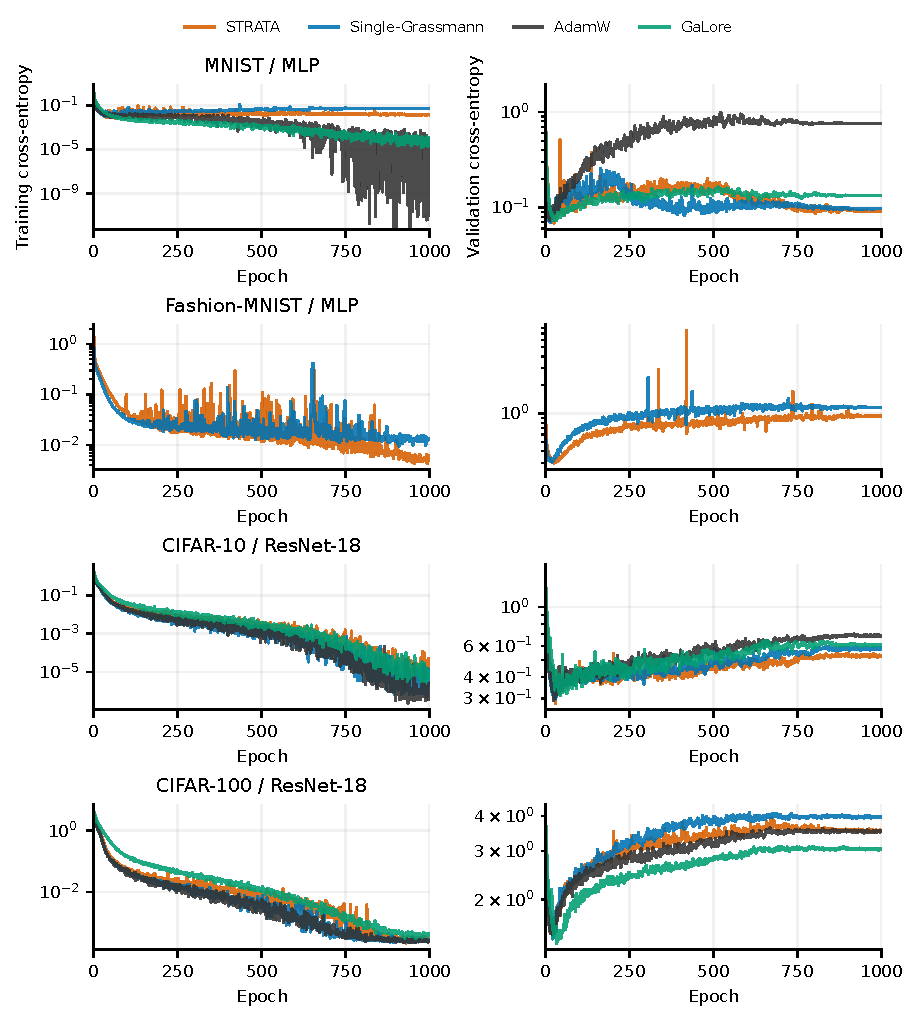
\includegraphics[width=.98\linewidth]{figures/fig_loss_classification_validation.pdf}
\caption{\textbf{Training and validation cross-entropy for the selected classifiers.} Each row is one dataset; left: training loss; right: held-out validation loss. The same selected run supplies both panels. A declining training loss with rising validation loss is retained. Missing Fashion-MNIST baselines are left absent. These are single-seed archived trajectories with unequal baseline search sizes.}
\label{fig:loss-classification-validation}
\end{figure}
\begin{figure}[!htbp]
\centering
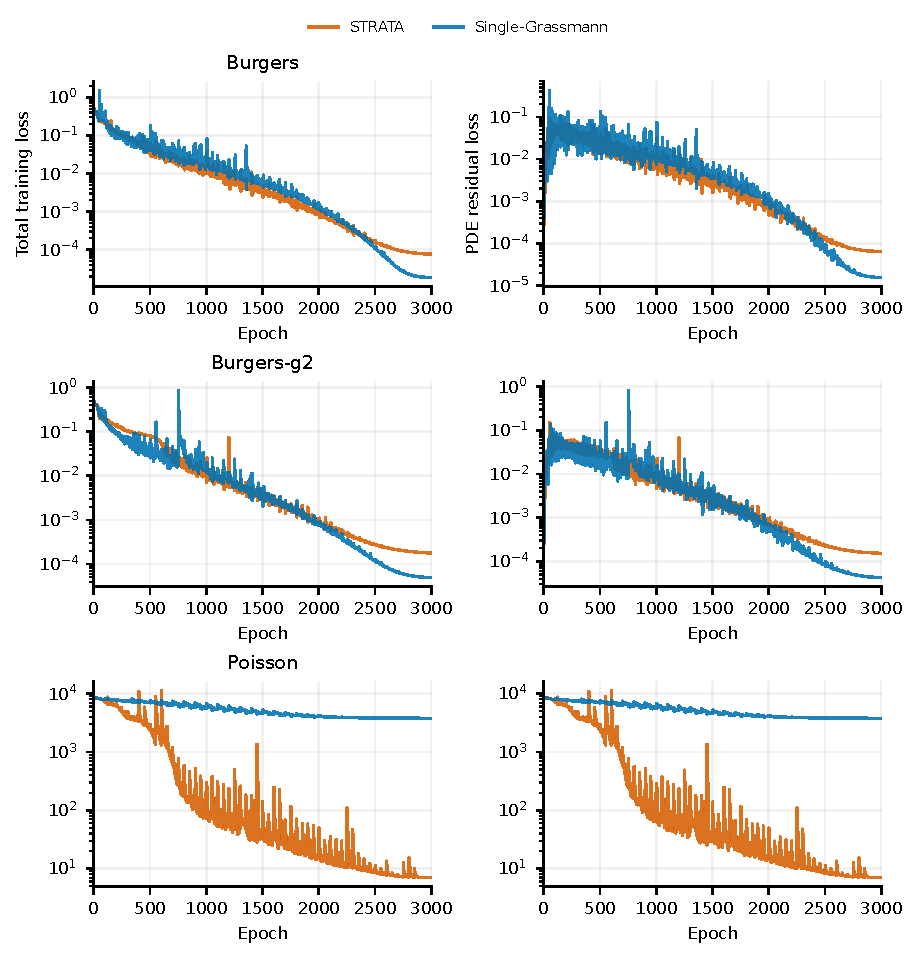
\includegraphics[width=.98\linewidth]{figures/fig_loss_scientific.pdf}
\caption{\textbf{Scientific-ML convergence at a strictly matched maximum rank of 64.} Left: total training loss; right: PDE residual loss. Exact-solution endpoint errors are tabulated separately. Rows: Burgers, Burgers-g2, Poisson. Each method's learning rate is selected by terminal PDE loss within rank 64. For Poisson this gives Single-Grassmann 2.04357 and STRATA 0.18741. The former differs from 2.00280, the rank-32 winner of the pooled-rank Single-Grassmann grid. Neither exact-solution error nor a favorable intermediate point selects a run.}
\label{fig:loss-scientific}
\end{figure}
\begin{figure}[!htbp]
\centering
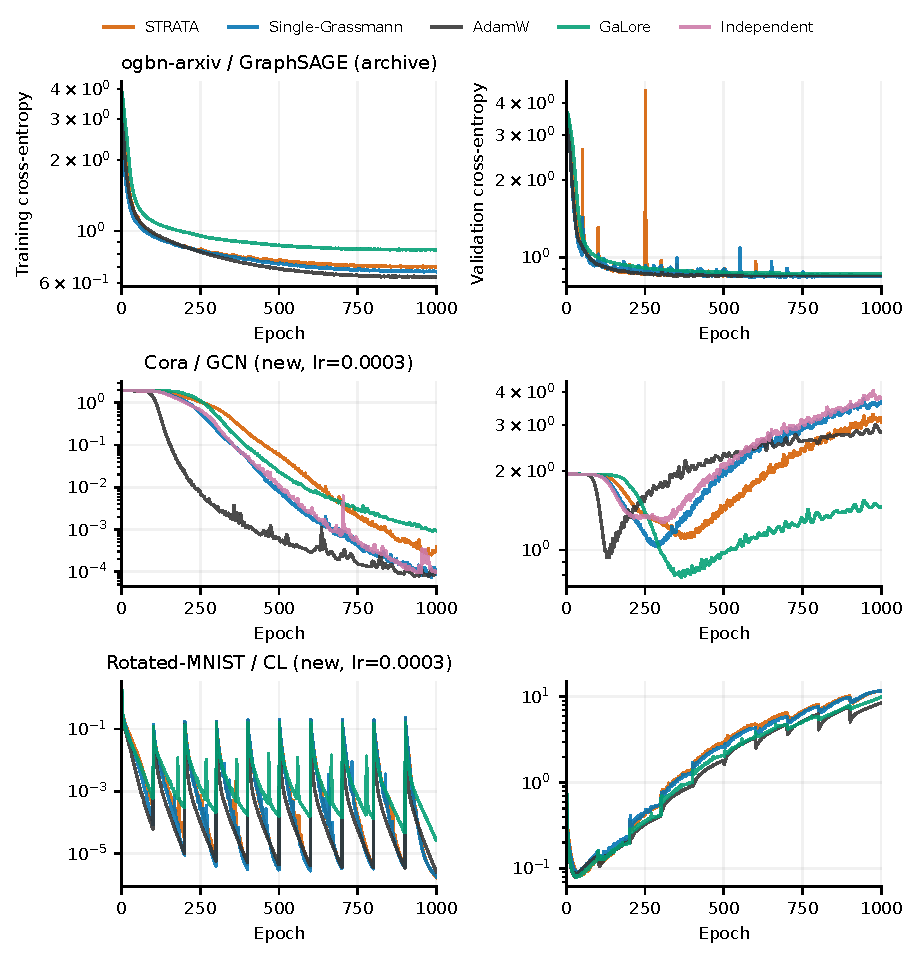
\includegraphics[width=.98\linewidth]{figures/fig_loss_graph_continual.pdf}
\caption{\textbf{Graph and continual-learning loss trajectories.} Left: training cross-entropy; right: validation cross-entropy. Rows show archived ogbn-arxiv, newly completed Cora/GCN configurations at the fixed rate $3\times10^{-4}$, and newly completed Rotated-MNIST fine-tuning configurations at that same fixed rate. In continual learning the held-out loss averages seen tasks, whose set grows at task boundaries; it is not the loss on an unchanging distribution. Only completed configurations are included in these panels.}
\label{fig:loss-graph-cl}
\end{figure}
\begin{figure}[!htbp]
\centering
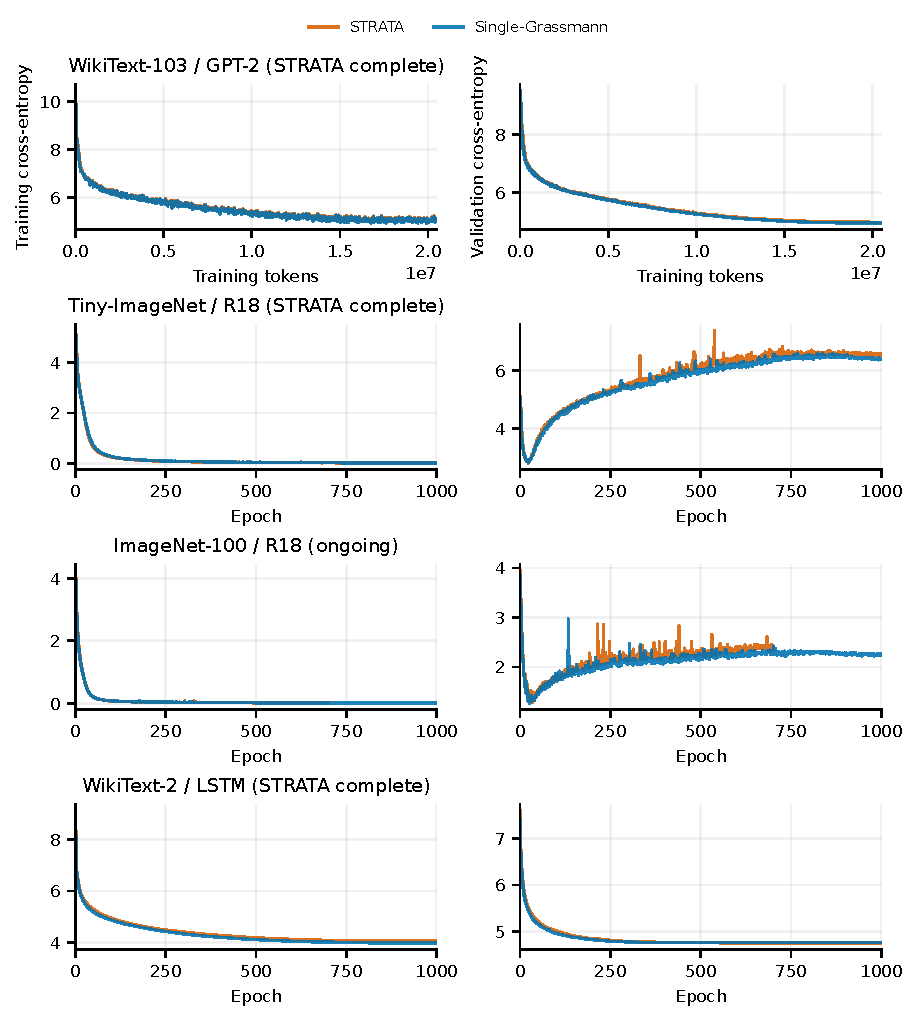
\includegraphics[width=.98\linewidth]{figures/fig_loss_ongoing.pdf}
\caption{\textbf{Large-task trajectories and configuration completion status.} Left: training loss; right: validation loss. Rows show WikiText-103/GPT-2, Tiny-ImageNet/ResNet-18, ImageNet-100/ResNet-18, and WikiText-2/LSTM at rate $3\times10^{-4}$. GPT-2 uses actual training tokens; the other rows use observed epochs. Each WikiText-2 epoch covers the complete next-token training corpus. A title marks any completed STRATA configuration; missing methods and unfinished searches do not become completed comparison cohorts. Other traces stop at their last observed epoch. A missing method has no available trace at the snapshot. The different language tokenizations also prevent interpreting perplexity across the two language-model rows as a matched comparison. These traces do not establish a family-level advantage.}
\label{fig:loss-ongoing}
\end{figure}
\begin{figure}[!htbp]
\centering
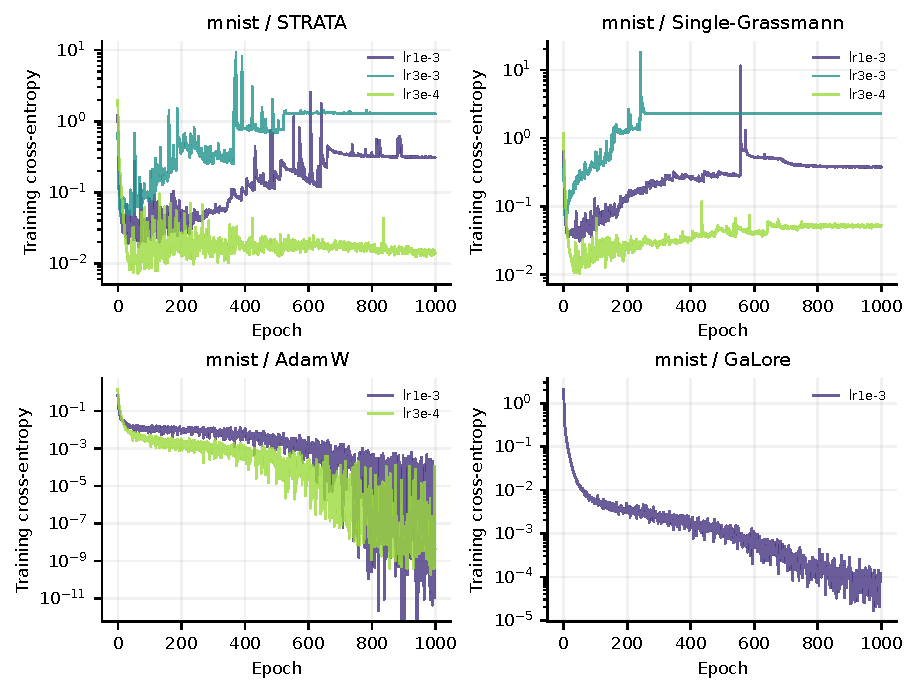
\includegraphics[width=.98\linewidth]{figures/fig_loss_grid_mnist.pdf}
\caption{\textbf{All completed MNIST classifier-grid training losses.} Separate panels show methods; lines show all available completed learning-rate trials. Poor configurations are retained. A 397-epoch partial GaLore trial is excluded from the complete-grid view.}
\end{figure}
\begin{figure}[!htbp]
\centering
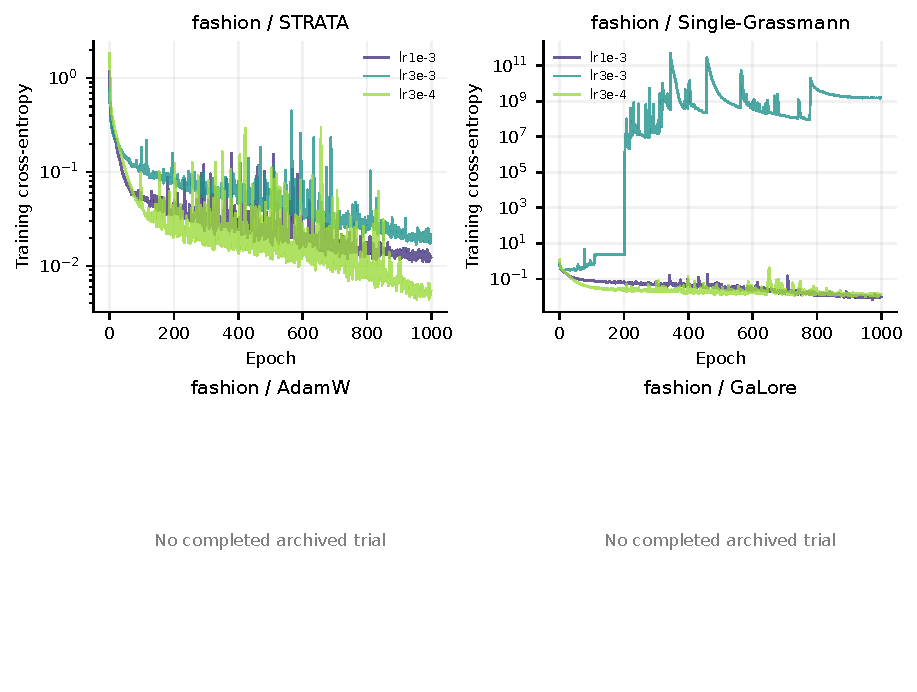
\includegraphics[width=.98\linewidth]{figures/fig_loss_grid_fashion.pdf}
\caption{\textbf{All completed Fashion-MNIST classifier-grid training losses.} Missing archived AdamW/GaLore grids are absent. The unstable Single-Grassmann trial remains visible rather than being removed from the learning-rate matrix.}
\end{figure}
\begin{figure}[!htbp]
\centering
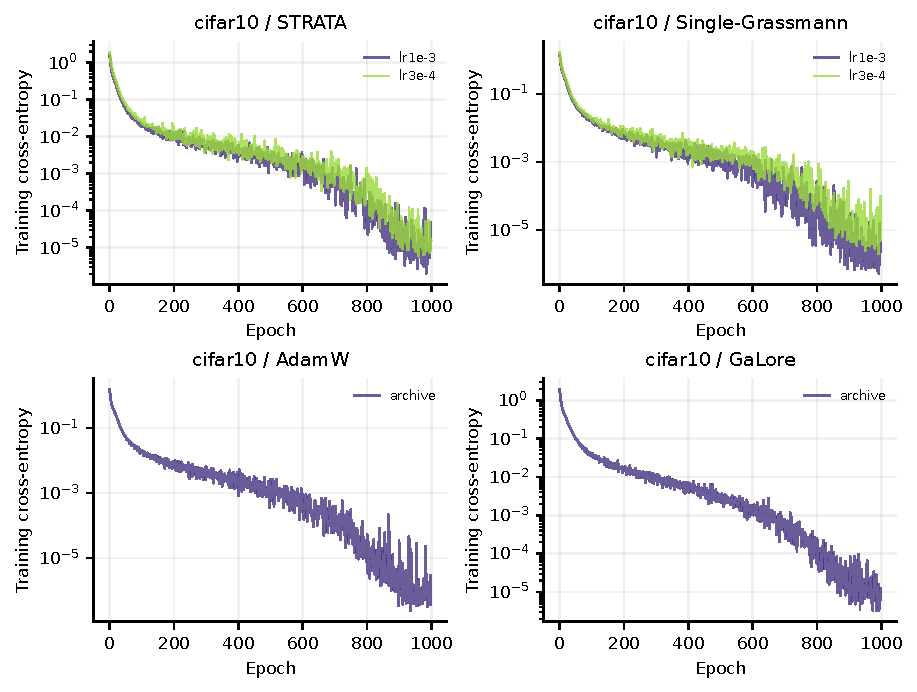
\includegraphics[width=.98\linewidth]{figures/fig_loss_grid_cifar10.pdf}
\caption{\textbf{All completed CIFAR-10 classifier-grid training losses.} STRATA/Single-Grassmann have two available rates; each archived AdamW/GaLore reference has one. These unequal grids are disclosed rather than represented as equal hyperparameter budgets.}
\end{figure}
\begin{figure}[!htbp]
\centering
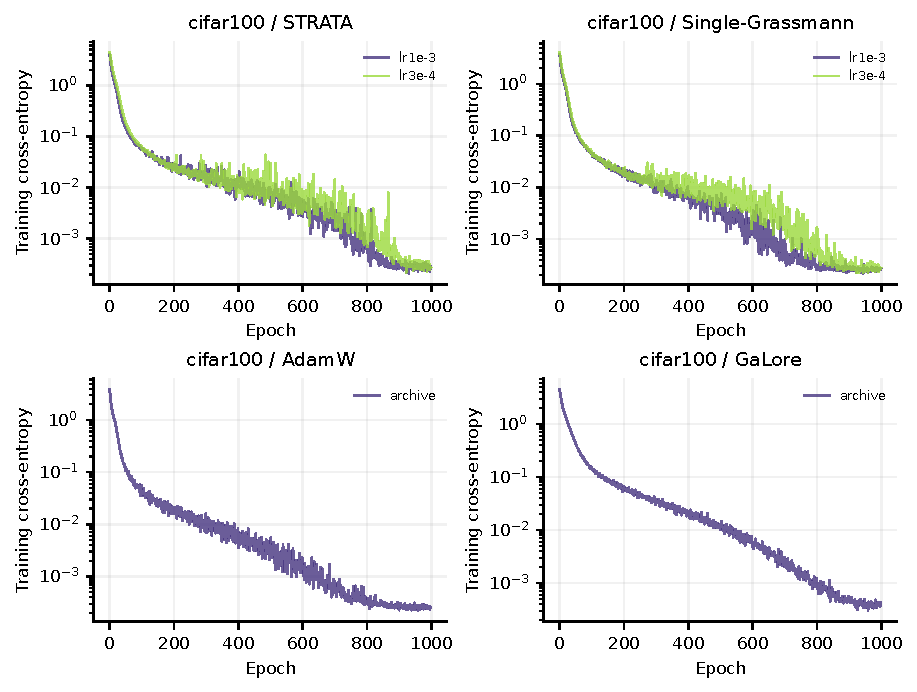
\includegraphics[width=.98\linewidth]{figures/fig_loss_grid_cifar100.pdf}
\caption{\textbf{All completed CIFAR-100 classifier-grid training losses.} The full training paths support optimization diagnostics while the held-out panels prevent interpreting a small terminal training loss as evidence of superior generalization.}
\end{figure}
\begin{longtable}{llrrrr}
\caption{Selected classifier convergence diagnostics. AUC integrates raw training loss over the observed archived epoch indices (0--999); $g_{\rm log}$ is the mean logged gradient norm, not a claim to the exact full-objective gradient. Missing gradient norms were not recorded in those archives and are left absent. Configurations use the selection rule of Figure~\ref{fig:loss-classification}.}\\
\toprule Dataset & Method & Loss AUC & Train loss & Val loss & $g_{\rm log}$\\\midrule\endfirsthead
\toprule Dataset & Method & Loss AUC & Train loss & Val loss & $g_{\rm log}$\\\midrule\endhead
\rowcolor{oursbg}
mnist & strata & 21.9 & 0.0144 & 0.0917 & 4.92 \\
mnist & single & 40.8 & 0.0513 & 0.0969 & 15.8 \\
mnist & adamw & 6.13 & 7.5e-05 & 0.759 & -- \\
mnist & galore & 7.21 & 7.76e-05 & 0.133 & 0.0133 \\
\rowcolor{oursbg}
fashion & strata & 35.2 & 0.0059 & 0.939 & 0.639 \\
fashion & single & 32.4 & 0.0131 & 1.16 & 1.99 \\
\rowcolor{oursbg}
cifar10 & strata & 19.4 & 1.77e-05 & 0.527 & 0.00133 \\
cifar10 & single & 16 & 4.69e-06 & 0.578 & 0.000361 \\
cifar10 & adamw & 17.4 & 3.19e-06 & 0.688 & -- \\
cifar10 & galore & 27.3 & 1.81e-05 & 0.607 & -- \\
\rowcolor{oursbg}
cifar100 & strata & 59 & 0.000286 & 3.56 & 0.00343 \\
cifar100 & single & 49.2 & 0.000261 & 3.98 & 0.00111 \\
cifar100 & adamw & 48.7 & 0.000259 & 3.53 & -- \\
cifar100 & galore & 101 & 0.000407 & 3.05 & -- \\
\bottomrule\end{longtable}


\paragraph{Breadth relative to the ManifoldFlow evaluation.}
The graph additions use custom 256-wide models: attention is single-head, SAGE-style aggregation uses the stated symmetric adjacency, and GCNII-style initial/identity mixing is fixed. These are controlled architecture variants, not reproductions of canonical published endpoints. The reference evaluation combines recurrent language models, tabular and image MLPs, a small Transformer, convolutional heads, component ablations, and scaling diagnostics. Our expanded matrix adds UCI Adult~\citep{uciAdult1996}, Covertype~\citep{uciCovertype1998}, red/white Wine Quality~\citep{uciWine2009} with 256- and 512-wide two-hidden-layer MLPs, and WikiText-2~\citep{merity2016pointer} with two-layer LSTM, two-layer GRU and a two-block Transformer. All five adaptive/projection methods receive rates $3\times10^{-4}$ and $10^{-3}$. Every formal tabular and sequence trial is prescribed 1000 complete epochs. These 110 additional configurations enlarge planned coverage; only completed entries in Appendix~\ref{app:new-completions} count as results.
\paragraph{Preprocessing and language budgets.}
Adult retains the official test split and hashes 10\% of official training for validation. Wine uses separate red/white tasks with target quality $\ge6$; identical full rows share a fixed 70/15/15 hash split. Covertype uses all 581012 records with the same hash split rule. All feature means, scales, and categorical dictionaries are fitted on training only. The WikiText-2 vocabulary is fitted on its official training split, with minimum frequency two and at most 30000 words. Its frozen splits contain 2088628/217646/245569 tokens. Every new sequence epoch visits the complete next-token training corpus; recurrent state is reset between contiguous blocks. This differs explicitly from the separate GPT-2 fixed-ten-step evaluation units. All preprocessing hashes and source revisions are retained.
\paragraph{Mechanistic ablations.}
A further 40 trials compare ten STRATA variants on Adult and red Wine Quality at both rates, keeping the same data, architecture, and full horizon. The full method, K=1, independent subspaces and full AdamW controls are reused from the matched tabular cohorts. Equal versus heterogeneous $(\beta_1,\beta_2)$ is a meaningful memory comparison: the heterogeneous variant uses $(.99,.9,.5)$ and $(.999,.99,.9)$, while the default has equal decays. The learned flag freezes after 200 updates in the freeze variant; this implementation also stops refresh-time variance resets, so it is a refresh-policy intervention rather than an isolated basis-motion change. The periodic-SVD variant refreshes a nested eigenspace chain of the pooled multi-timescale covariance; pooling changes its flag objective, so it is a baseline rather than a pure retraction-only intervention. Least-squares transport uses $M^+=MU_{\rm old}^\top U_{\rm new}$ and is distinguished from both the implemented rotation and omission of rotation. Remaining variants equalize/reverse covariance memories, equalize coefficients, remove the residual, fix a random flag, or omit transport. Each new code path is smoke-tested before formal activation; smoke runs never count as completed evidence.

\FloatBarrier
\subsection{New completed breadth-cohort loss curves}
\label{app:breadth-loss-updates}
Every displayed cohort contains five completed full-budget methods. Learning rates are selected on validation only after both predeclared rates have completed for every method; otherwise a completed common-rate cohort is labeled fixed-rate. Each curve is traced to its complete log in the accompanying audit.
\begin{figure}[!htbp]
\centering
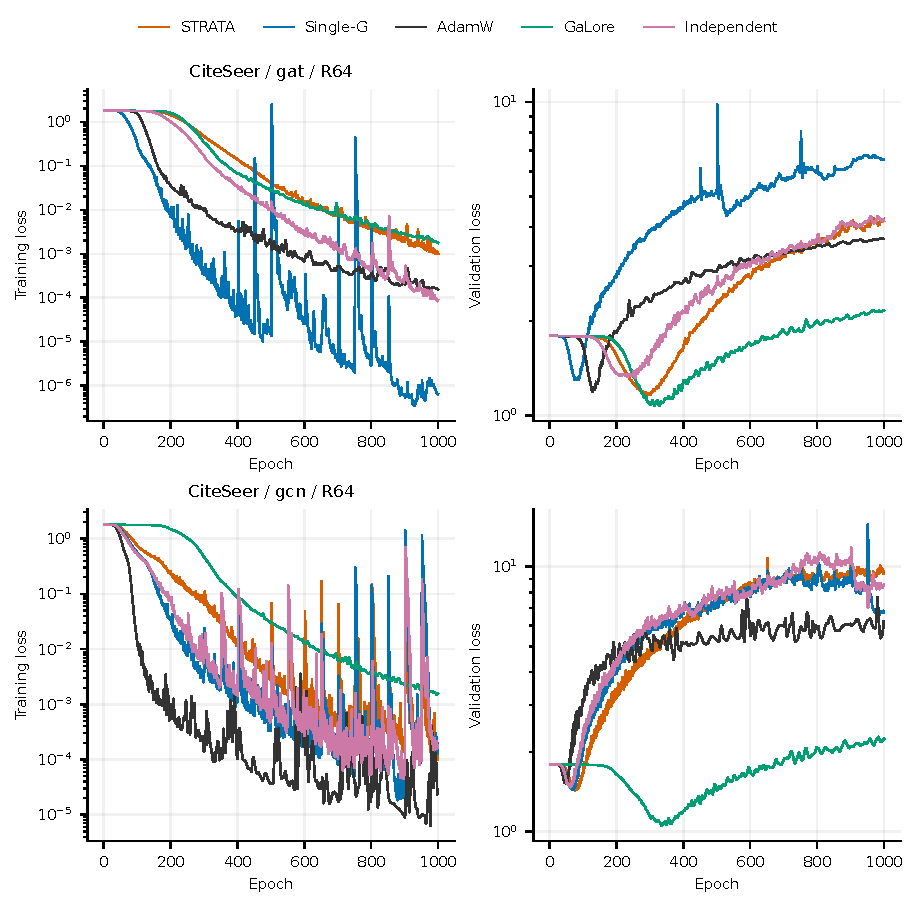
\includegraphics[width=.98\linewidth]{figures/fig_breadth_complete_00.pdf}
\caption{\textbf{Completed breadth-cohort training and validation losses.} CiteSeer/gat: two-rate validation selection; CiteSeer/gcn: two-rate validation selection. Left: training; right: validation. Raw complete trajectories, seed 42. No smoothing or extrapolation.}
\end{figure}
\begin{figure}[!htbp]
\centering
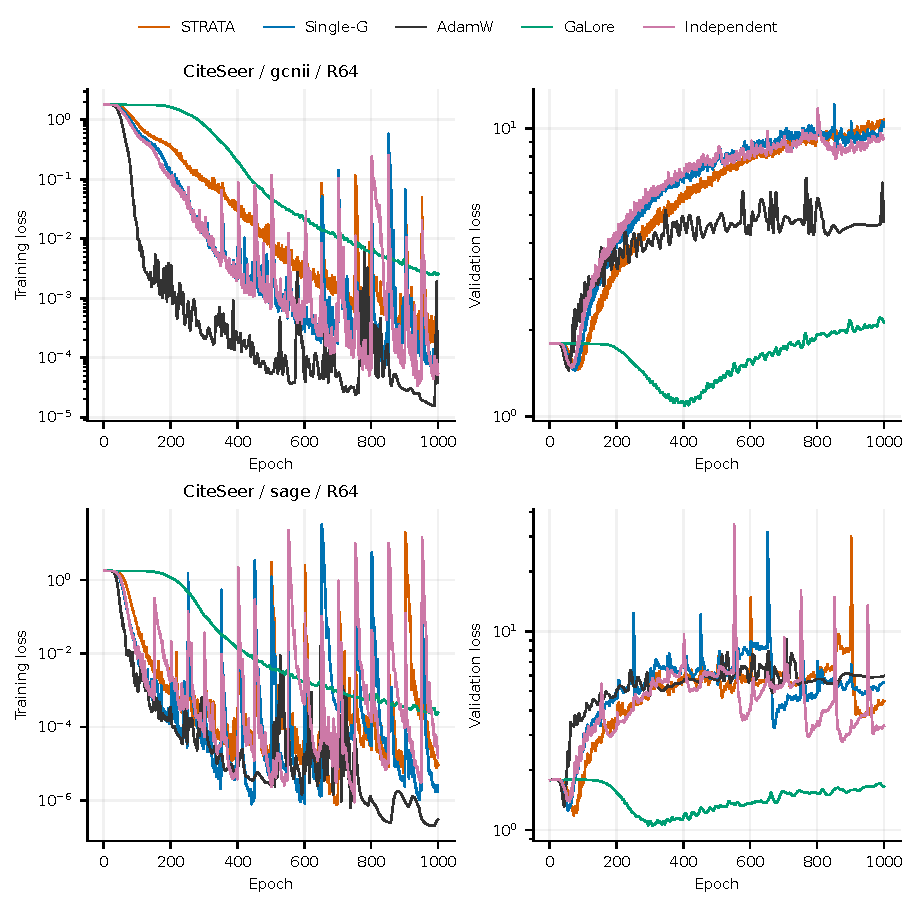
\includegraphics[width=.98\linewidth]{figures/fig_breadth_complete_01.pdf}
\caption{\textbf{Completed breadth-cohort training and validation losses.} CiteSeer/gcnii: two-rate validation selection; CiteSeer/sage: two-rate validation selection. Left: training; right: validation. Raw complete trajectories, seed 42. No smoothing or extrapolation.}
\end{figure}
\begin{figure}[!htbp]
\centering
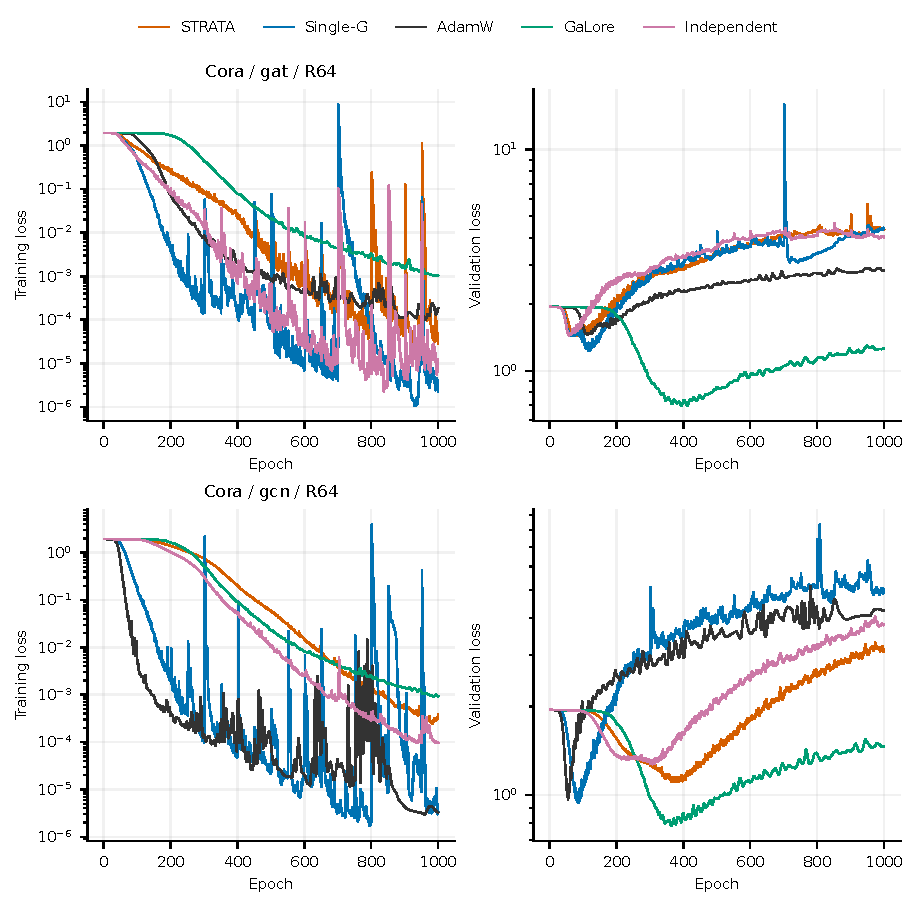
\includegraphics[width=.98\linewidth]{figures/fig_breadth_complete_02.pdf}
\caption{\textbf{Completed breadth-cohort training and validation losses.} Cora/gat: two-rate validation selection; Cora/gcn: two-rate validation selection. Left: training; right: validation. Raw complete trajectories, seed 42. No smoothing or extrapolation.}
\end{figure}
\begin{figure}[!htbp]
\centering
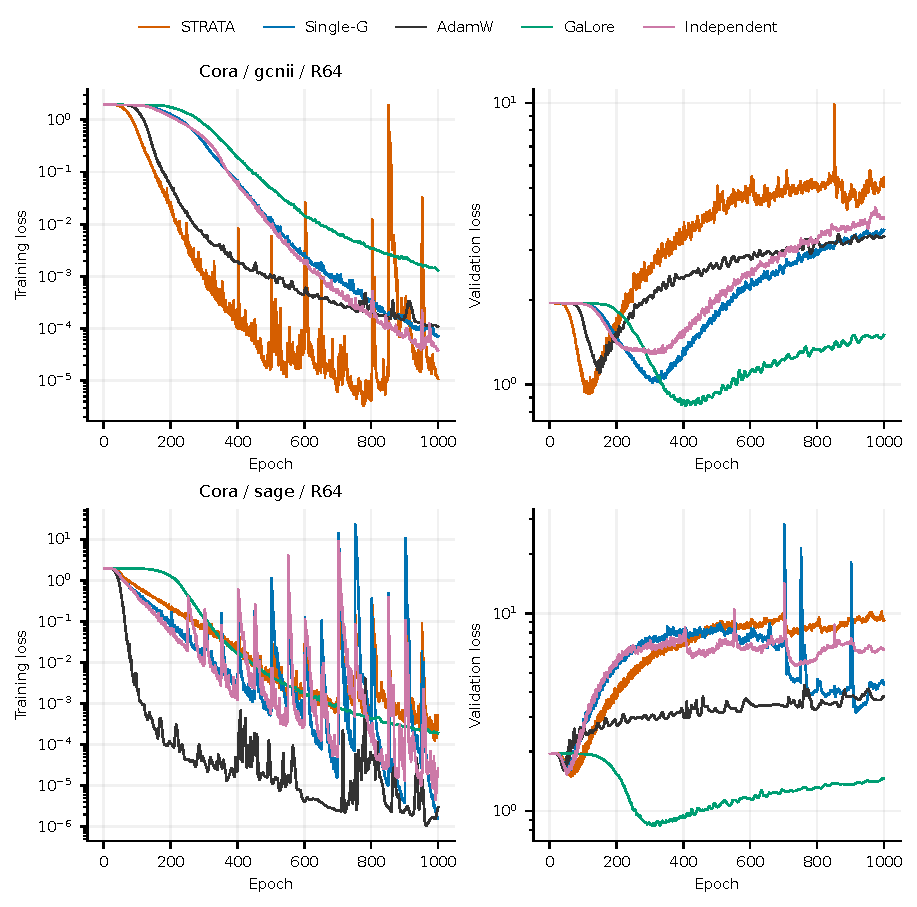
\includegraphics[width=.98\linewidth]{figures/fig_breadth_complete_03.pdf}
\caption{\textbf{Completed breadth-cohort training and validation losses.} Cora/gcnii: two-rate validation selection; Cora/sage: two-rate validation selection. Left: training; right: validation. Raw complete trajectories, seed 42. No smoothing or extrapolation.}
\end{figure}
\begin{figure}[!htbp]
\centering
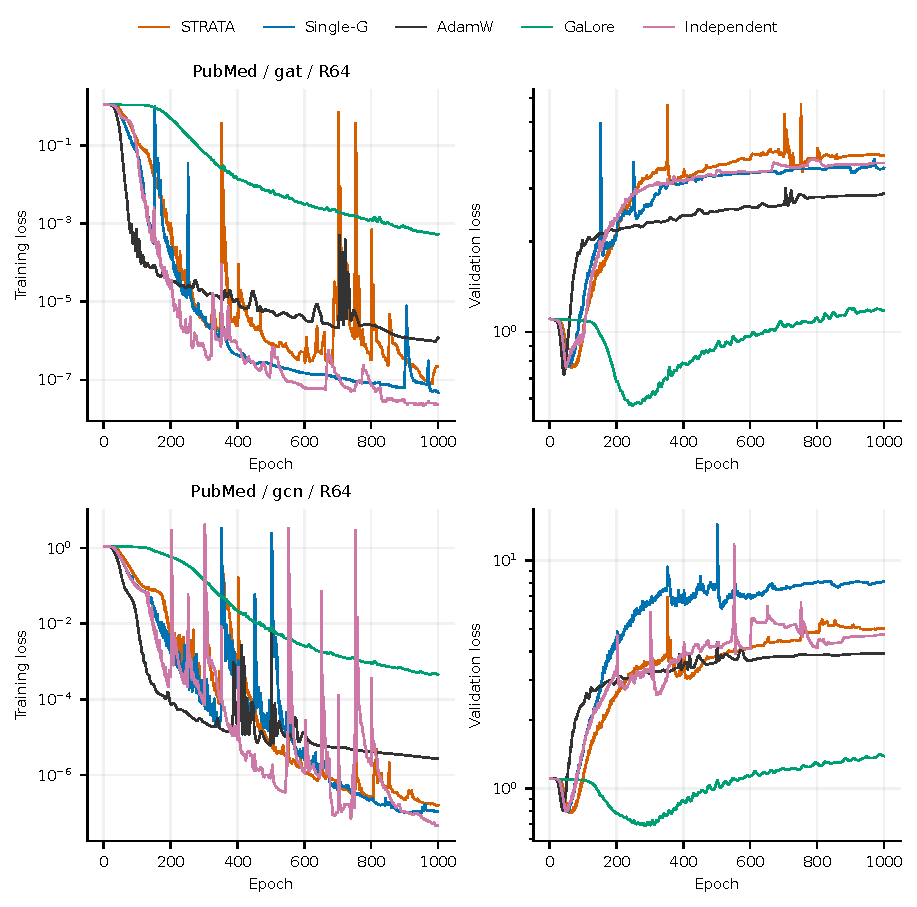
\includegraphics[width=.98\linewidth]{figures/fig_breadth_complete_04.pdf}
\caption{\textbf{Completed breadth-cohort training and validation losses.} PubMed/gat: two-rate validation selection; PubMed/gcn: two-rate validation selection. Left: training; right: validation. Raw complete trajectories, seed 42. No smoothing or extrapolation.}
\end{figure}
\begin{figure}[!htbp]
\centering
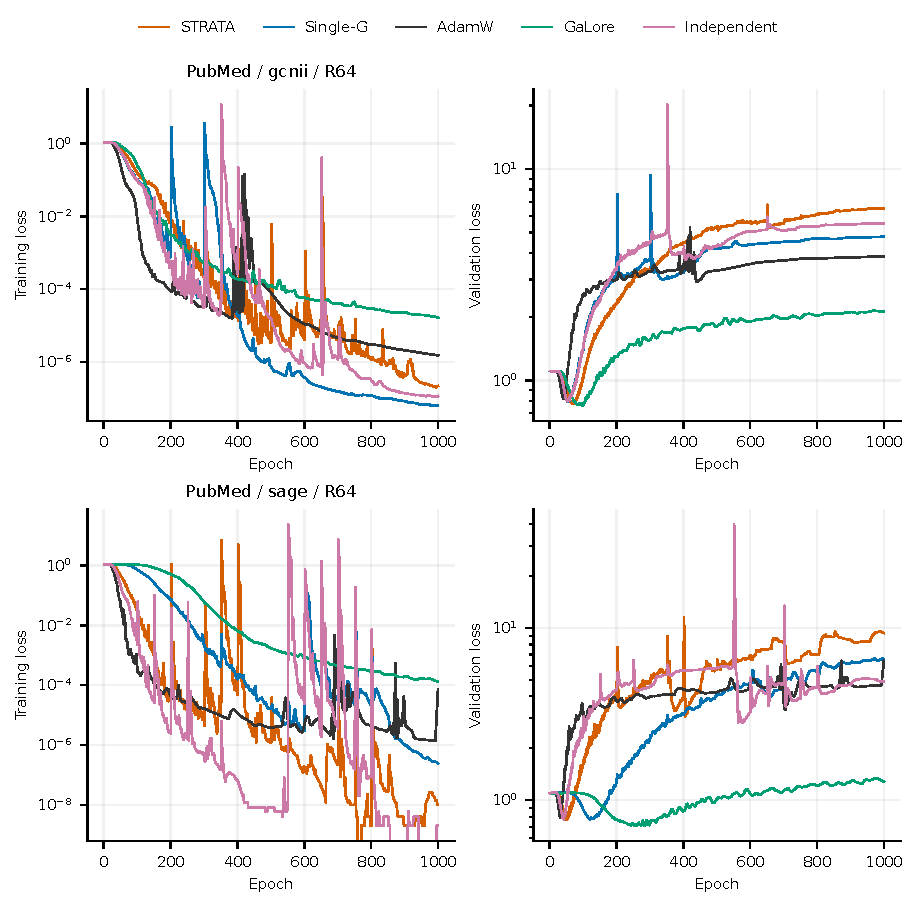
\includegraphics[width=.98\linewidth]{figures/fig_breadth_complete_05.pdf}
\caption{\textbf{Completed breadth-cohort training and validation losses.} PubMed/gcnii: two-rate validation selection; PubMed/sage: two-rate validation selection. Left: training; right: validation. Raw complete trajectories, seed 42. No smoothing or extrapolation.}
\end{figure}
\begin{figure}[!htbp]
\centering
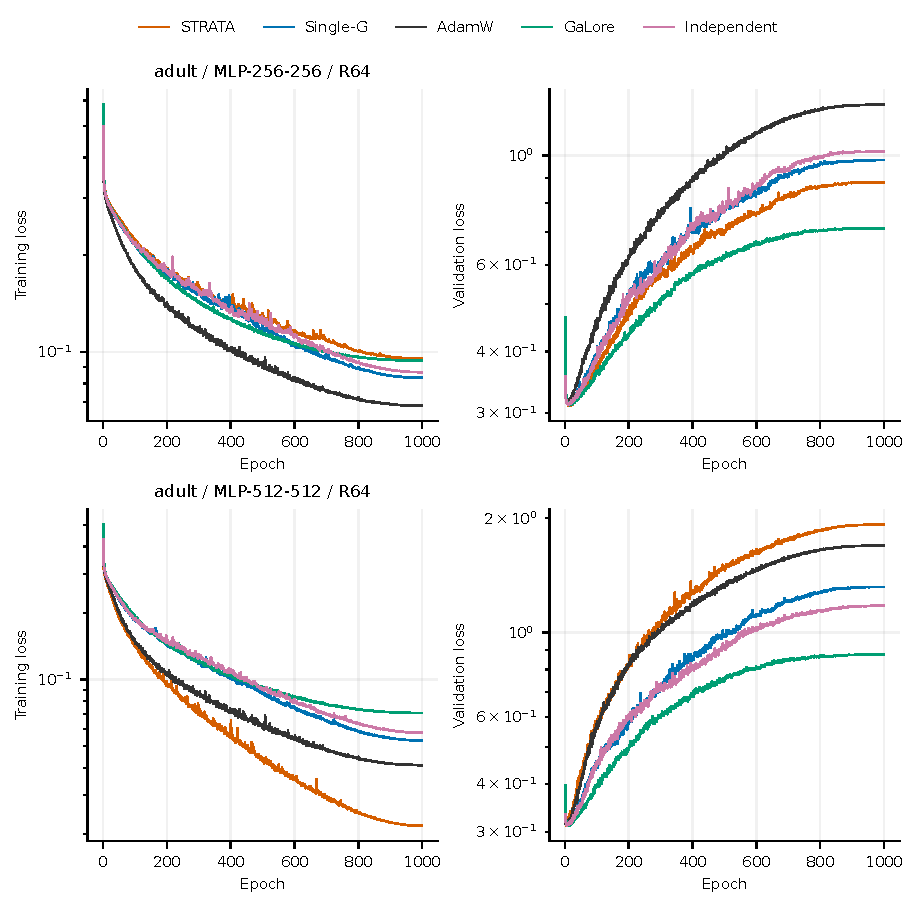
\includegraphics[width=.98\linewidth]{figures/fig_breadth_complete_06.pdf}
\caption{\textbf{Completed breadth-cohort training and validation losses.} adult/MLP-256-256: two-rate validation selection; adult/MLP-512-512: two-rate validation selection. Left: training; right: validation. Raw complete trajectories, seed 42. No smoothing or extrapolation.}
\end{figure}
\begin{figure}[!htbp]
\centering
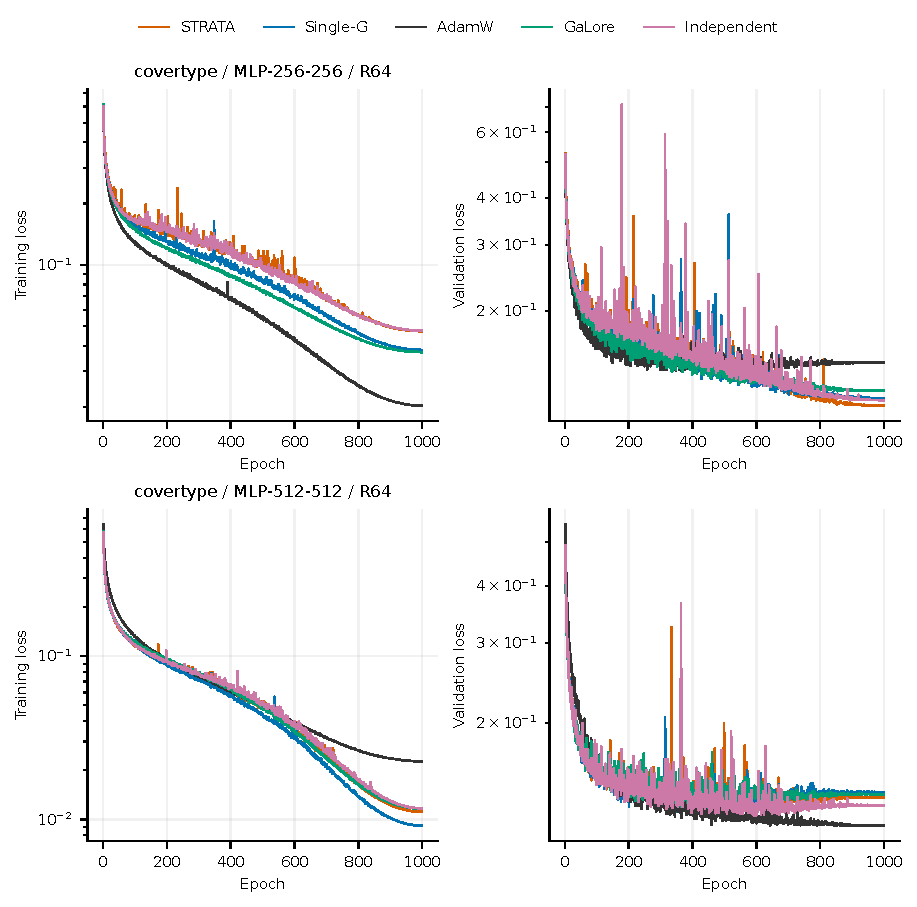
\includegraphics[width=.98\linewidth]{figures/fig_breadth_complete_07.pdf}
\caption{\textbf{Completed breadth-cohort training and validation losses.} covertype/MLP-256-256: two-rate validation selection; covertype/MLP-512-512: two-rate validation selection. Left: training; right: validation. Raw complete trajectories, seed 42. No smoothing or extrapolation.}
\end{figure}
\begin{figure}[!htbp]
\centering
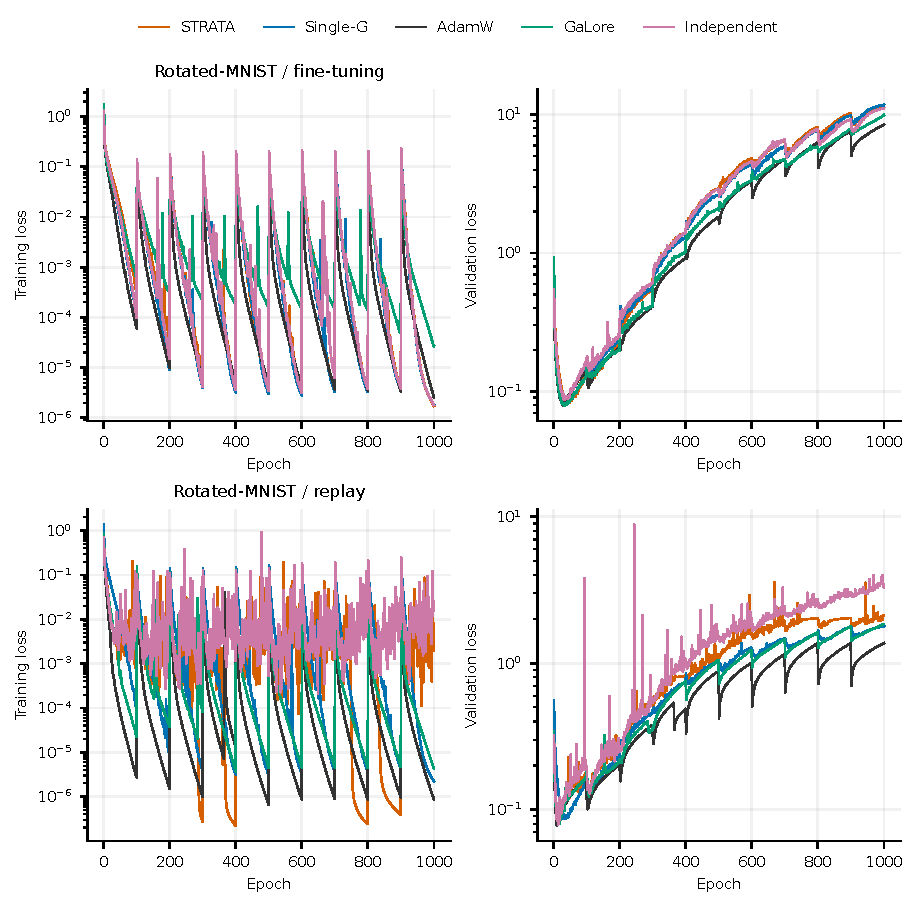
\includegraphics[width=.98\linewidth]{figures/fig_breadth_complete_08.pdf}
\caption{\textbf{Completed breadth-cohort training and validation losses.} rotated\_mnist\_cl/MLP-256-256/finetune: two-rate validation selection; rotated\_mnist\_cl/MLP-256-256/replay: two-rate validation selection. Left: training; right: validation. Raw complete trajectories, seed 42. Continual validation averages seen tasks, so its evaluation distribution changes at task boundaries. No smoothing or extrapolation.}
\end{figure}
\begin{figure}[!htbp]
\centering
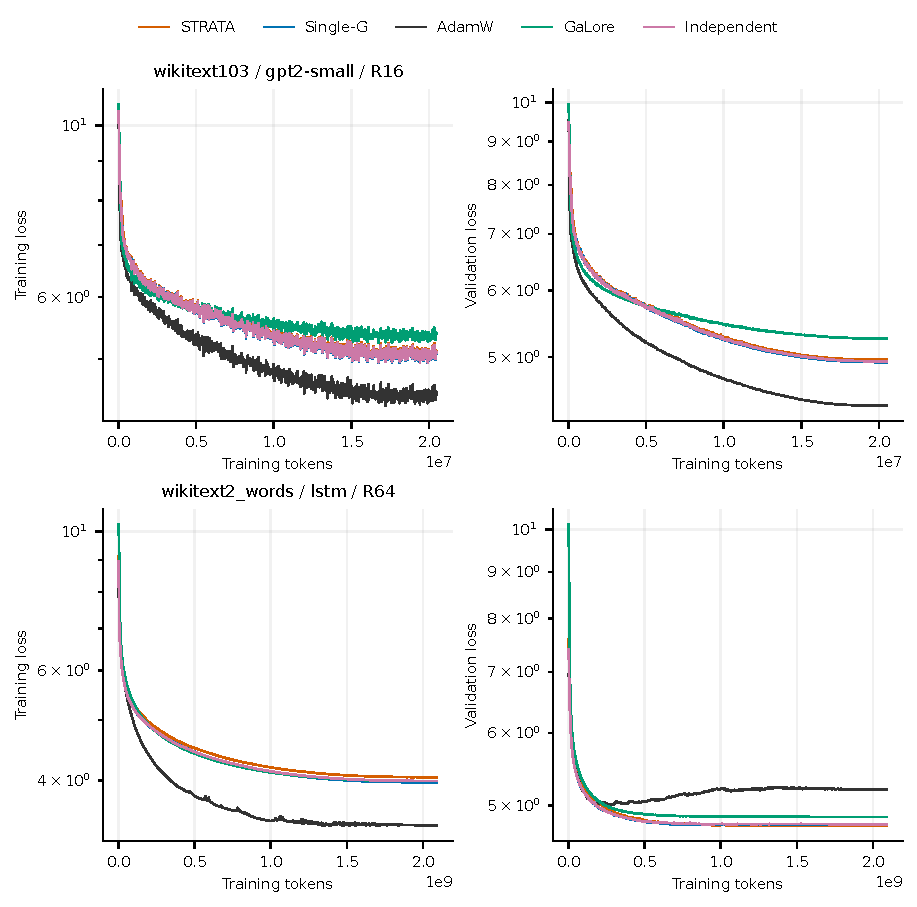
\includegraphics[width=.98\linewidth]{figures/fig_breadth_complete_09.pdf}
\caption{\textbf{Completed breadth-cohort training and validation losses.} wikitext103/gpt2-small: two-rate validation selection; wikitext2\_words/lstm: fixed rate 0.0003; search incomplete. Left: training; right: validation. Raw complete trajectories, seed 42. No smoothing or extrapolation.}
\end{figure}
\begin{figure}[!htbp]
\centering
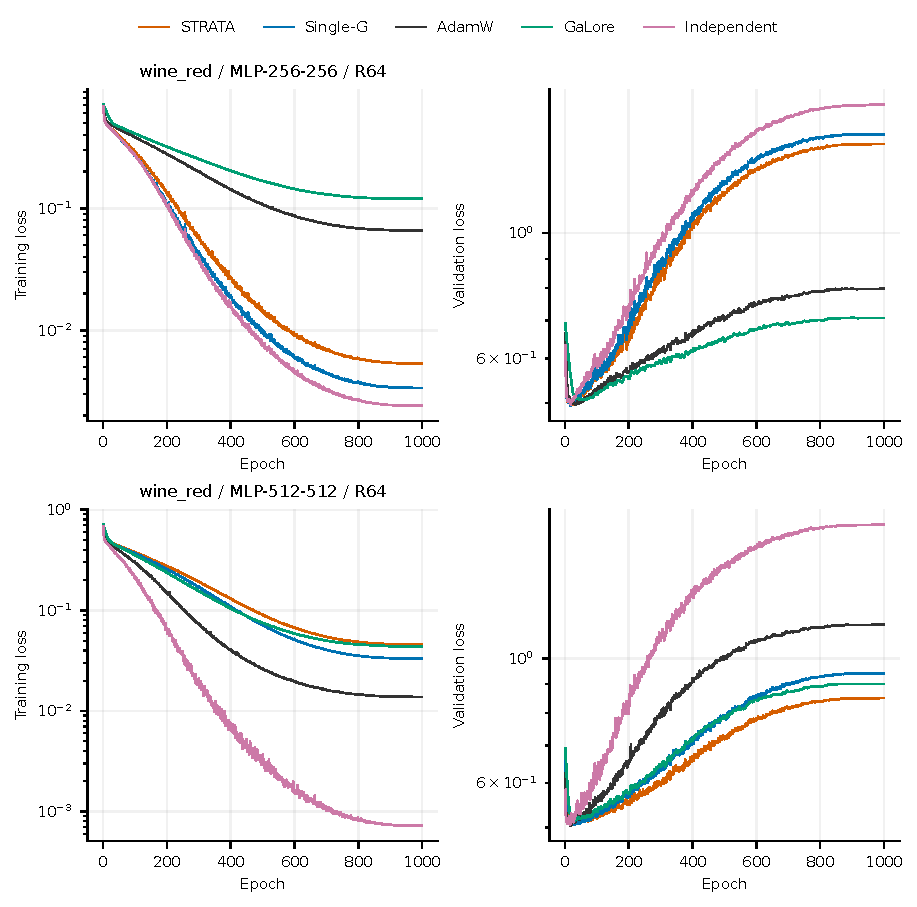
\includegraphics[width=.98\linewidth]{figures/fig_breadth_complete_10.pdf}
\caption{\textbf{Completed breadth-cohort training and validation losses.} wine\_red/MLP-256-256: two-rate validation selection; wine\_red/MLP-512-512: two-rate validation selection. Left: training; right: validation. Raw complete trajectories, seed 42. No smoothing or extrapolation.}
\end{figure}
\begin{figure}[!htbp]
\centering
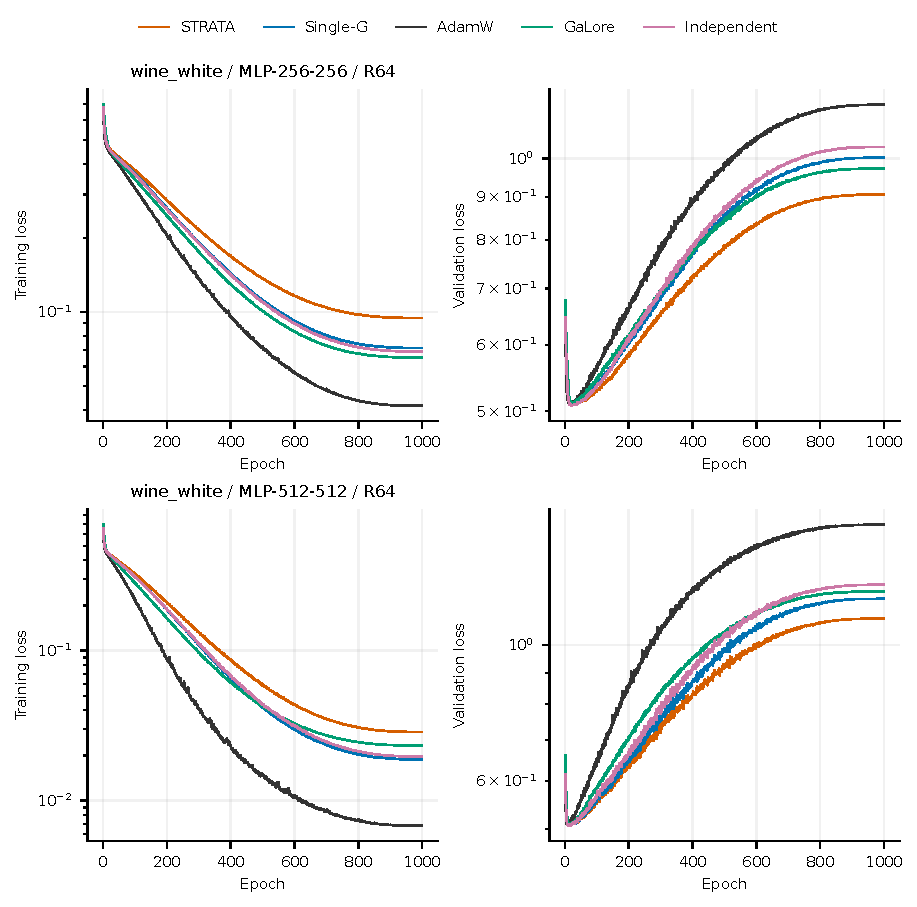
\includegraphics[width=.98\linewidth]{figures/fig_breadth_complete_11.pdf}
\caption{\textbf{Completed breadth-cohort training and validation losses.} wine\_white/MLP-256-256: two-rate validation selection; wine\_white/MLP-512-512: two-rate validation selection. Left: training; right: validation. Raw complete trajectories, seed 42. No smoothing or extrapolation.}
\end{figure}


\FloatBarrier
\subsection{Completed ablation loss trajectories}
Each panel uses one predeclared fixed learning rate and only full-budget completed runs. The ablation matrix may still be incomplete; missing variants are not assigned values. All completed variants, including adverse ones, are retained.
\begin{figure}[!htbp]
\centering
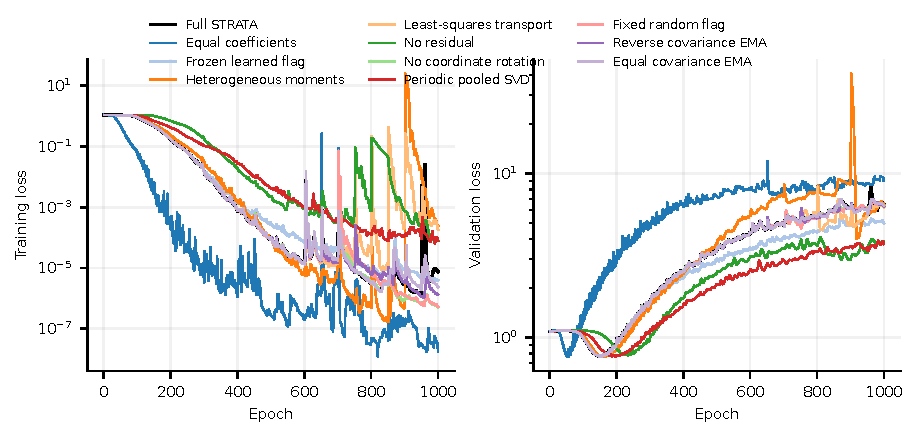
\includegraphics[width=.98\linewidth]{figures/fig_ablation_complete_f4222fea23ff.pdf}
\caption{\textbf{Completed fixed-rate ablation trajectories.} PubMed/sage/64/0.0003. Left: training; right: validation. Raw losses for the full method and every currently completed variant, seed 42. No smoothing, test selection or extrapolation. In continual learning the validation set averages seen tasks.}
\end{figure}
\begin{figure}[!htbp]
\centering
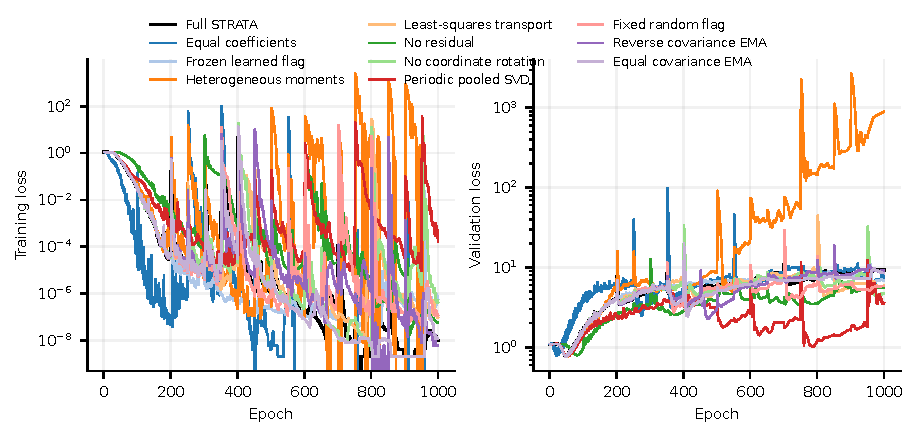
\includegraphics[width=.98\linewidth]{figures/fig_ablation_complete_92ad161e923b.pdf}
\caption{\textbf{Completed fixed-rate ablation trajectories.} PubMed/sage/64/0.001. Left: training; right: validation. Raw losses for the full method and every currently completed variant, seed 42. No smoothing, test selection or extrapolation. In continual learning the validation set averages seen tasks.}
\end{figure}
\begin{figure}[!htbp]
\centering
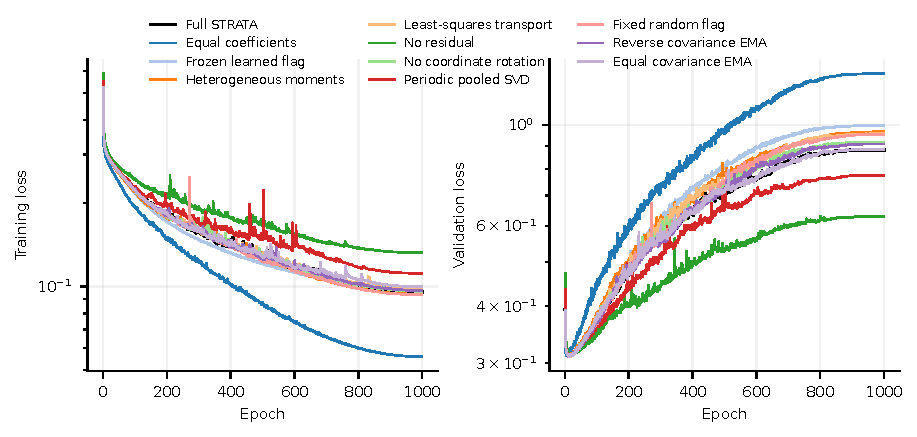
\includegraphics[width=.98\linewidth]{figures/fig_ablation_complete_cd63c9d43c42.pdf}
\caption{\textbf{Completed fixed-rate ablation trajectories.} adult/MLP-256-256/64/0.0003. Left: training; right: validation. Raw losses for the full method and every currently completed variant, seed 42. No smoothing, test selection or extrapolation. In continual learning the validation set averages seen tasks.}
\end{figure}
\begin{figure}[!htbp]
\centering
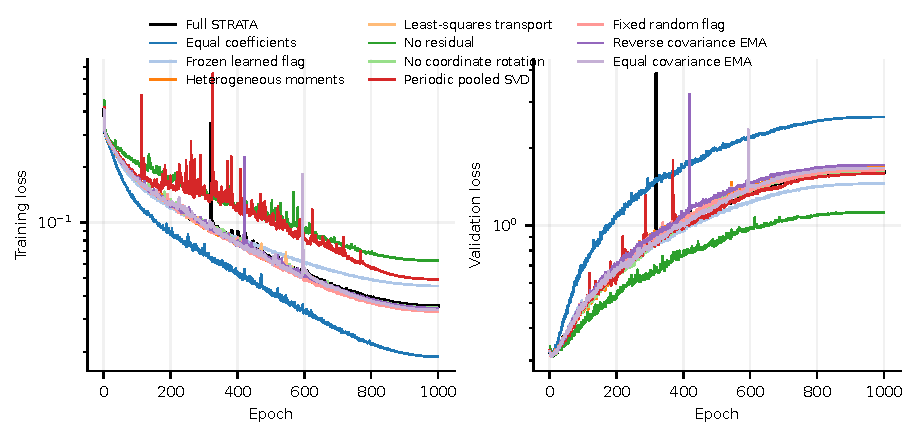
\includegraphics[width=.98\linewidth]{figures/fig_ablation_complete_f1b02595ebb0.pdf}
\caption{\textbf{Completed fixed-rate ablation trajectories.} adult/MLP-256-256/64/0.001. Left: training; right: validation. Raw losses for the full method and every currently completed variant, seed 42. No smoothing, test selection or extrapolation. In continual learning the validation set averages seen tasks.}
\end{figure}
\begin{figure}[!htbp]
\centering
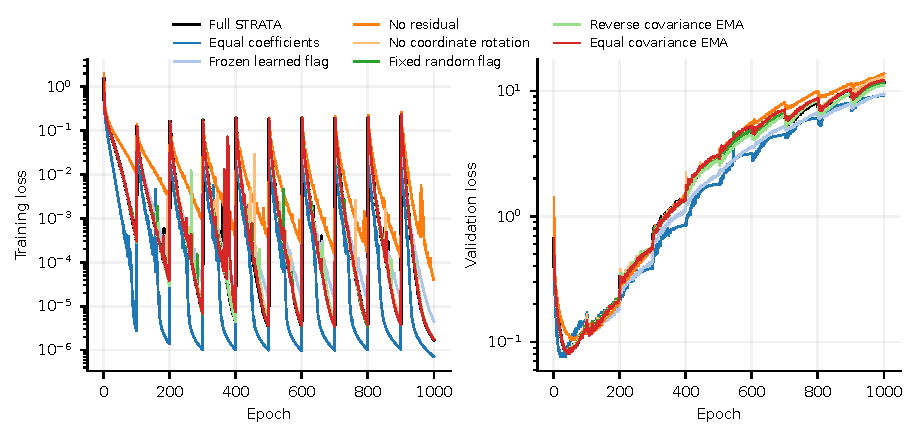
\includegraphics[width=.98\linewidth]{figures/fig_ablation_complete_22095cc4347a.pdf}
\caption{\textbf{Completed fixed-rate ablation trajectories.} rotated\_mnist\_cl/MLP-256-256/64/0.0003. Left: training; right: validation. Raw losses for the full method and every currently completed variant, seed 42. No smoothing, test selection or extrapolation. In continual learning the validation set averages seen tasks.}
\end{figure}
\begin{figure}[!htbp]
\centering
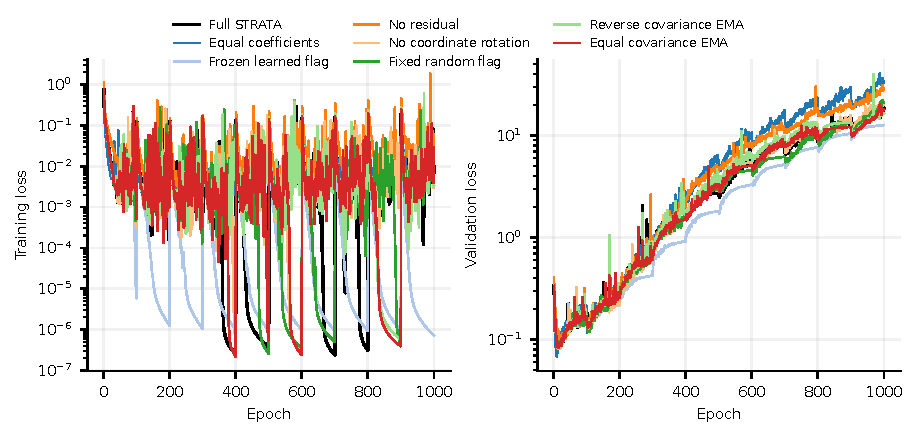
\includegraphics[width=.98\linewidth]{figures/fig_ablation_complete_4cf87464d8ba.pdf}
\caption{\textbf{Completed fixed-rate ablation trajectories.} rotated\_mnist\_cl/MLP-256-256/64/0.001. Left: training; right: validation. Raw losses for the full method and every currently completed variant, seed 42. No smoothing, test selection or extrapolation. In continual learning the validation set averages seen tasks.}
\end{figure}
\begin{figure}[!htbp]
\centering
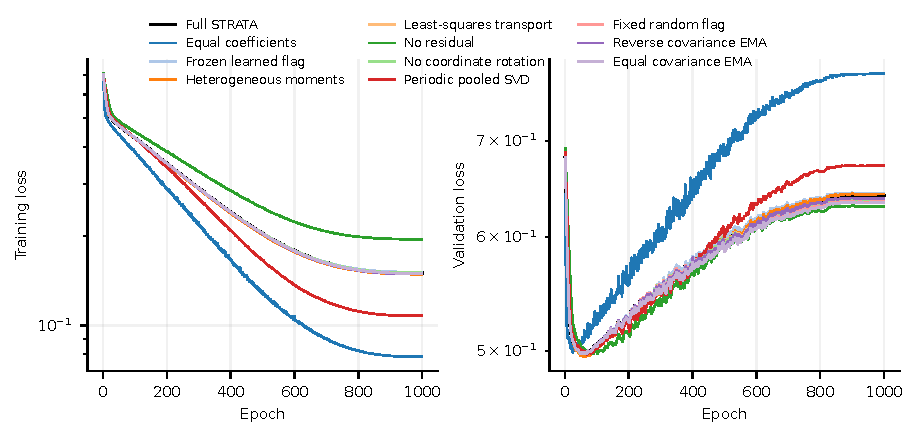
\includegraphics[width=.98\linewidth]{figures/fig_ablation_complete_6327e4845709.pdf}
\caption{\textbf{Completed fixed-rate ablation trajectories.} wine\_red/MLP-256-256/64/0.0003. Left: training; right: validation. Raw losses for the full method and every currently completed variant, seed 42. No smoothing, test selection or extrapolation. In continual learning the validation set averages seen tasks.}
\end{figure}
\begin{figure}[!htbp]
\centering
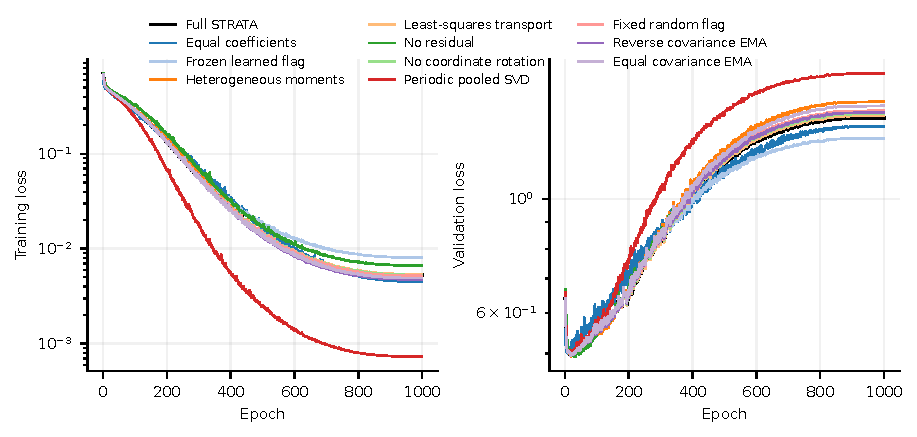
\includegraphics[width=.98\linewidth]{figures/fig_ablation_complete_f7dd6296b414.pdf}
\caption{\textbf{Completed fixed-rate ablation trajectories.} wine\_red/MLP-256-256/64/0.001. Left: training; right: validation. Raw losses for the full method and every currently completed variant, seed 42. No smoothing, test selection or extrapolation. In continual learning the validation set averages seen tasks.}
\end{figure}


\section{Diagnostics of the Actual Adaptive-Update Theory}
\label{app:actual-theory-diagnostics}
\begin{table}[htbp]
\centering
\caption{\textbf{Exact normalization-bias counterexample.} Symmetric and asymmetric zero-mean noises have variance $\sigma^2$, $\sigma=.3$. The true optimum is zero. The asymmetric stationary root is given by Proposition~\ref{prop:actual-skew-counterexample}.}
\label{tab:actual-normalization}
\begin{adjustbox}{max width=\linewidth}
\begin{tabular}{rrr}
\toprule
$\epsilon$ & Symmetric root & Asymmetric root \\
\midrule
0.0001 & 0 & 0.09998750 \\
0.001 & 0 & 0.09987514 \\
0.01 & 0 & 0.09876392 \\
0.1 & 0 & 0.08877693 \\
1 & 0 & 0.04300047 \\
10 & 0 & 0.00676348 \\
\bottomrule
\end{tabular}
\end{adjustbox}
\end{table}
\begin{table}[htbp]
\centering
\caption{\textbf{Finite-trajectory diagnostics at $\epsilon=.01$.} Means use the final 5000 of 30000 seed-42 stochastic-approximation iterates. These are finite-run observations, not asymptotic estimates.}
\label{tab:normalization-tail}
\begin{adjustbox}{max width=\linewidth}
\begin{tabular}{lr}
\toprule
Update / noise & Final-5000 mean $w$ \\
\midrule
Normalized / skew & 0.09878739 \\
Normalized / symmetric & 0.06416802 \\
SGD / skew & 0.00508841 \\
SGD / symmetric & 0.00119654 \\
\bottomrule
\end{tabular}
\end{adjustbox}
\end{table}

\paragraph{Implementation-level identity checks.}
A float64 test calls the unmodified STRATA matrix update for 100 steps with 20 flag refreshes on an $8\times6$ matrix, ranks $(1,2,3)$ and nonidentical moment decays. It reconstructs the ambient moment, exact adaptive direction, and virtual iterate using the actual stored states. Maximum identity errors are $2.18\times10^{-16}$, $2.20\times10^{-15}$, and $3.56\times10^{-17}$, respectively. These tests exercise the exact identities in Proposition~\ref{prop:actual-momentum} and Theorem~\ref{thm:actual-convergence}, including refresh steps; they do not assert that the variation budgets vanish on neural benchmarks. The analytic asymmetric root has update-field residual $6.3\times10^{-15}$. One hundred scalar posterior-variance checks give maximum first-order residual $5.4\times10^{-15}$ and nonnegative refinement gains, checking Theorem~\ref{thm:directional-pac} and Proposition~\ref{prop:directional-refinement}. Source hashes and complete numerical outputs are retained.
\begin{table}[htbp]
\centering
\caption{\textbf{Implementation-level variation-budget checks.} The float64 trajectory has 100 steps and 20 flag refreshes. Maxima summarize each sequence separately; inequalities are checked step by step. A violation means slack below $-10^{-10}$.}
\label{tab:actual-state-budgets}
\begin{adjustbox}{max width=\linewidth}
\begin{tabular}{lrrrrr}
\toprule
Quantity & Steps & Max observed & Max bound & Min slack & Violations \\
\midrule
Preconditioner & 99 & 7.231e+01 & 1.443e+03 & +1.049e+02 & 0 \\
Momentum coefficient & 99 & 4.737e-01 & 1.302e+00 & +1.019e-11 & 0 \\
Transport defect & 100 & 4.782e-03 & 8.445e-02 & -1.242e-16 & 0 \\
\bottomrule
\end{tabular}
\end{adjustbox}
\end{table}
\begin{table}[htbp]
\centering
\caption{\textbf{Exact adaptive-update identities.} Maximum residual over the same 100-step trajectory.}
\label{tab:actual-identities}
\begin{adjustbox}{max width=\linewidth}
\begin{tabular}{lr}
\toprule
Identity & Maximum residual \\
\midrule
ambient momentum & 2.173e-16 \\
exact direction & 2.199e-15 \\
virtual iterate & 3.560e-17 \\
\bottomrule
\end{tabular}
\end{adjustbox}
\end{table}



\FloatBarrier
\section{Completed Evidence, Resource Audits, and Controlled Follow-ups}\label{app:evidence-extension}
All comparisons below use seed 42. A two-rate result requires both rates for every method, and all prescribed epochs must finish. Rates and exploratory flag-step settings are selected on validation only. Incomplete configurations remain in the execution counts, without extrapolated endpoints.
\paragraph{Proposal coverage and remaining work.} Configuration counts measure execution coverage, not positive results. The graph and tabular grids are complete; image and continual-learning runs continue; the LSTM grid has nine completed candidates and one recorded failure. WikiText-2 epochs traverse its full corpus; GPT-2 uses fixed ten-step evaluation units, explicitly not corpus epochs or the 1000-corpus-epoch-equivalent proposal budget. OpenWebText/C4 subsets and corpus-switch experiments are not established completed benchmarks in this matrix. Core50 and DomainNet acquisition is complete, but readiness does not imply completion of their long-horizon runs.
\begin{table}[htbp]\centering\footnotesize\setlength{\tabcolsep}{3pt}\caption{Execution snapshot by disjoint queue family. No pending, running, deferred or failed configuration is a completed endpoint.}\label{tab:evidence-coverage}\begin{adjustbox}{max width=\linewidth}
\begin{tabular}{lrrrrrr}\toprule Family & Complete & Running & Pending & Deferred & Data wait & Failed\\\midrule
ablation & 54 & 0 & 0 & 0 & 0 & 0 \\
continual & 22 & 5 & 5 & 68 & 0 & 0 \\
forecasting & 60 & 0 & 0 & 0 & 0 & 0 \\
graph & 120 & 0 & 0 & 0 & 0 & 0 \\
graph mechanism/sweep & 38 & 0 & 0 & 0 & 0 & 0 \\
language & 10 & 0 & 0 & 92 & 0 & 0 \\
nonstationary & 30 & 0 & 0 & 0 & 0 & 0 \\
recommendation & 60 & 0 & 0 & 0 & 0 & 0 \\
scientific & 10 & 0 & 0 & 0 & 0 & 0 \\
sensor\_drift & 60 & 0 & 0 & 0 & 0 & 0 \\
sequence & 9 & 0 & 0 & 20 & 0 & 1 \\
tabular & 80 & 0 & 0 & 0 & 0 & 0 \\
vision & 3 & 2 & 9 & 98 & 0 & 0 \\
\bottomrule\end{tabular}
\end{adjustbox}\end{table}
\paragraph{Compute-scope revision (2026-11-04).}\label{app:reduced-scope}
After observing the earlier exploratory comparisons, we reduced the remaining computational scope. The original 856-configuration ledger is preserved: 278 unstarted configurations are explicitly deferred, not counted as completed or removed according to their eventual result. All seven jobs already running at the decision remain unchanged; no trajectory is shortened, and all retained formal runs still require 1000 epochs. Thirty pending configurations remain eligible, leaving 37 unfinished runs at the decision. This is an adaptive exploratory scope revision, not completion of the original full proposal grid.

The priority is to complete the existing Rotated-MNIST fine-tuning grid and its replay extension, motivated by the earlier comparison-specific continual-learning gain and the multi-timescale memory hypothesis. Both retain five methods and both original rates. For ResNet-18 on ImageNet-100, Tiny-ImageNet, DomainNet, and CORe50, the retained comparison uses one rate per method: the first-listed rate in the original queue, fixed without selecting among their test outcomes. All original methods are retained within each setting, including SGD with momentum and Muon in the two image-classification settings. These four groups support fixed-rate comparisons only, not validation-selected two-rate claims. Additional already-running rates remain individual configurations and do not alter that rule.

\begin{table}[htbp]\centering\footnotesize
\caption{\textbf{Retained scope after compute reduction.} Counts below are full comparison candidates, including already completed or running members. Priority determines execution order, not inclusion of favorable outcomes. Every completed comparator, including stronger baselines, remains reportable.}\label{tab:reduced-scope}
\begin{tabular}{llrrl}\toprule Setting & Model/base & Methods & Candidates & Rate protocol\\\midrule
Rotated-MNIST & MLP/fine-tuning & 5 & 10 & Two original rates\\
Rotated-MNIST & MLP/replay & 5 & 10 & Two original rates\\
ImageNet-100 & ResNet-18 & 7 & 7 & Fixed first-listed rate\\
Tiny-ImageNet & ResNet-18 & 7 & 7 & Fixed first-listed rate\\
DomainNet & ResNet-18/fine-tuning & 5 & 5 & Fixed first-listed rate\\
CORe50 & ResNet-18/fine-tuning & 5 & 5 & Fixed first-listed rate\\
\bottomrule\end{tabular}\end{table}

For the five adaptive/projection methods, the fixed rate is $3\times10^{-4}$; image SGD and Muon use their original first-listed rates $0.03$ and $0.01$, respectively. The Rotated-MNIST search retains $\{3\times10^{-4},10^{-3}\}$ per method. Deferred work includes larger vision architectures, additional GPT-2 model/rank grids, GRU/Transformer sequence variants, and the unstarted EWC and other replay expansions. Deferral is a scope decision and supplies no evidence for or against STRATA. The LSTM candidate already in progress at the scope revision has since completed; its failed AdamW candidate remains visible below.

\paragraph{Recorded numerical failure.} The WikiText-2/LSTM AdamW candidate at learning rate $10^{-3}$ stopped at epoch 276 after training, validation, and test losses became non-finite. Its log contains 275 finite epochs of the prescribed 1000; it supplies no completed endpoint. Nine of the ten planned LSTM configurations are complete, including the final Independent candidate. The two-rate comparison remains incomplete because of this failed AdamW candidate. A completed common-rate subset, when displayed, is labeled fixed-rate rather than validation-selected.
\paragraph{Measured state--quality tradeoffs.} State includes every unique optimizer tensor storage in a final checkpoint, including fixed probes; weights, gradients and transient workspaces are separate. Peak allocation and shared-server timing are reported independently, so a reduction in stored state is not asserted to be a peak-memory or speed reduction.
{\footnotesize\setlength{\tabcolsep}{3pt}\begin{longtable}{llrrrr}\caption{Complete-cohort resource audit. Ratios compare STRATA with full AdamW after each method independently selects its learning rate on validation. Accuracy differences are STRATA minus Single-G; perplexity and relative-L2 differences retain their lower-is-better sign.}\\\toprule Task & Model & State ratio & Peak ratio & Test & $\Delta$ Single-G\\\midrule\endfirsthead\toprule Task & Model & State ratio & Peak ratio & Test & $\Delta$ Single-G\\\midrule\endhead
CiteSeer & gat & 0.402 & 0.983 & 0.56758 & -0.02417 \\
CiteSeer & gcn & 0.402 & 0.964 & 0.49199 & -0.02356 \\
CiteSeer & gcnii & 0.402 & 0.967 & 0.47508 & -0.02366 \\
CiteSeer & sage & 0.379 & 0.961 & 0.55747 & +0.01767 \\
Cora & gat & 0.559 & 0.992 & 0.69798 & -0.02111 \\
Cora & gcn & 0.558 & 0.977 & 0.70120 & -0.01523 \\
Cora & gcnii & 0.558 & 0.978 & 0.68975 & -0.01163 \\
Cora & sage & 0.478 & 0.968 & 0.46532 & -0.18529 \\
Darcy-generated & FNO & 1.027 & 1.003 & 0.13637 & +0.00807 \\
PubMed & gat & 0.782 & 1.000 & 0.71174 & -0.03134 \\
PubMed & gcn & 0.781 & 0.998 & 0.71742 & +0.00534 \\
PubMed & gcnii & 0.781 & 0.998 & 0.66341 & -0.04726 \\
PubMed & sage & 0.581 & 0.996 & 0.71623 & +0.03721 \\
adult & MLP-256-256 & 1.000 & 1.000 & 0.81486 & -0.00001 \\
adult & MLP-512-512 & 0.535 & 0.986 & 0.81509 & +0.00227 \\
cifar100\_class\_shift & ResNet18-CIFAR & 0.244 & 0.979 & 0.53092 & -0.04278 \\
cifar10\_label\_shift & ResNet18-CIFAR & 0.241 & 0.979 & 0.75012 & -0.01638 \\
covertype & MLP-256-256 & 0.925 & 1.000 & 0.96224 & -0.00077 \\
covertype & MLP-512-512 & 0.513 & 0.994 & 0.96644 & +0.00002 \\
rotated\_mnist\_shift & MLP-256-256 & 0.578 & 0.997 & 0.97615 & -0.00281 \\
wikitext103 & gpt2-small & 0.040 & 0.822 & 144.54240 & +4.87039 \\
wine\_red & MLP-256-256 & 0.911 & 1.017 & 0.68421 & -0.00408 \\
wine\_red & MLP-512-512 & 0.469 & 1.019 & 0.71500 & +0.01798 \\
wine\_white & MLP-256-256 & 0.911 & 0.998 & 0.72423 & -0.00747 \\
wine\_white & MLP-512-512 & 0.469 & 0.957 & 0.70875 & -0.01435 \\
\bottomrule\end{longtable}}
\paragraph{Completed Darcy/FNO comparison.} All ten two-rate configurations finish 2000 epochs on the retained generated $16\times16$ operator dataset. Validation relative $L_2$ selects the rate; PDE residual and spectral errors are secondary test metrics. Frequency errors are mean squared FFT magnitudes of errors in training-standard-deviation target units. This is not an external standard Darcy benchmark. Spectral real/imaginary tensors retain dense Adam state; eligible pointwise matrices use projected state.
\begin{table}[htbp]\centering\footnotesize\setlength{\tabcolsep}{3pt}\caption{Completed generated-Darcy/FNO results, terminal-100 test metrics.}\label{tab:darcy-complete}\begin{adjustbox}{max width=\linewidth}
\begin{tabular}{lrrrrr}\toprule Method & lr & Rel-$L_2$ & PDE residual & Low-freq & High-freq\\\midrule
\rowcolor{oursbg}
STRATA & 1e-03 & 0.1364 & 3.45 & 274 & 0.115 \\
Single-G & 1e-03 & 0.1283 & 3.06 & 257 & 0.101 \\
AdamW & 1e-03 & 0.1146 & 2.17 & 206 & 0.1 \\
GaLore & 1e-03 & 0.1399 & 3.8 & 290 & 0.128 \\
Independent & 1e-03 & 0.1266 & 2.83 & 257 & 0.104 \\
\bottomrule\end{tabular}
\end{adjustbox}\end{table}
\begin{figure}[!htbp]\centering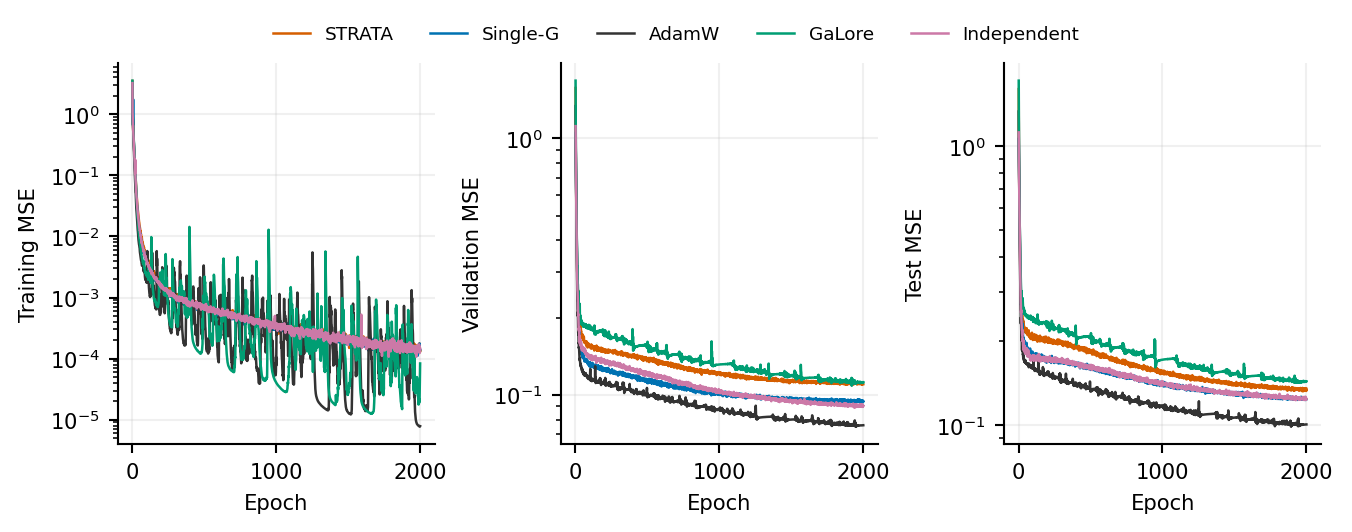
\includegraphics[width=.98\linewidth]{figures/fig_evidence_darcy.png}\caption{Complete 2000-epoch Darcy/FNO loss trajectories: training, validation, and test MSE. Rates are validation-selected from complete two-rate grids; test residual and spectrum never select a curve. All methods and adverse outcomes are retained.}\end{figure}
\paragraph{PubMed mechanism follow-up.} The ten variants and both rates are frozen before follow-up outcomes. Their controls reuse the original two full-method configurations. Freezing after 200 updates also stops variance resets; periodic pooled SVD changes the flag objective. Thus these are explicitly identified interventions, not pure isolated geometry controls.
\begin{table}[htbp]\centering\footnotesize\setlength{\tabcolsep}{3pt}\caption{Complete PubMed/SAGE ablation grid, validation-selected rates, terminal-100 accuracies. Differences are relative to full STRATA. No variant is promoted to the default based on test results.}\label{tab:pubmed-ablations}\begin{adjustbox}{max width=\linewidth}
\begin{tabular}{lrrrr}\toprule Variant & lr & Val & Test & $\Delta$ test (pp)\\\midrule
\rowcolor{oursbg}
full & 1e-03 & 0.71792 & 0.71623 & +0.000 \\
same\_rho & 1e-03 & 0.71302 & 0.70196 & -1.427 \\
reverse\_rho & 3e-04 & 0.69346 & 0.67923 & -3.700 \\
equal\_a & 1e-03 & 0.71646 & 0.71188 & -0.435 \\
no\_residual & 1e-03 & 0.70986 & 0.69363 & -2.260 \\
random\_flag & 1e-03 & 0.69942 & 0.70164 & -1.459 \\
no\_transport & 3e-04 & 0.69988 & 0.67823 & -3.800 \\
frozen\_after\_warmup & 3e-04 & 0.69730 & 0.67639 & -3.984 \\
heterogeneous\_memory & 1e-03 & 0.71310 & 0.70829 & -0.794 \\
periodic\_svd & 1e-03 & 0.70572 & 0.69553 & -2.070 \\
least\_squares\_transport & 1e-03 & 0.70994 & 0.70900 & -0.723 \\
\bottomrule\end{tabular}
\end{adjustbox}\end{table}
\paragraph{Exploratory flag-step sensitivity.} The declared grid is $\xi\in\{10^{-3},10^{-1},10\}$ and $\eta\in\{3\times10^{-4},10^{-3}\}$ for each of STRATA, Single-G and Independent: six equal-budget candidates per method. Defaults remain unchanged. Larger raw-objective steps test whether weak flag motion limits the default protocol. Baseline numerical paths were checked unchanged for all five optimizers over 55 paired updates; all 20 new graph-path smoke tests passed. New runs save float32 bases and evaluate span motion with float64 QR/SVD; old float16 flag snapshots are not used to infer tiny principal angles. The span diagnostic is $D_{\rm span}=\sqrt{1-\lVert Q_{10}^{\top}Q_{1000}\rVert_F^2/r}$, with fresh orthonormal QR factors and represented rank $r$. Independent uses the concatenated subspace union when it has full column rank; excluded rank-deficient matrices are not assigned zero motion.
\begin{table}[htbp]\centering\footnotesize\setlength{\tabcolsep}{3pt}\caption{Matched six-candidate exploratory search per geometric optimizer, selected on validation. Span motion compares the total represented space at checkpoints 10 and 1000, using float64 QR/SVD and averaging eligible matrices. It is not an oracle tracking error.}\label{tab:xi-sweep}\begin{adjustbox}{max width=\linewidth}
\begin{tabular}{lrrrrr}\toprule Method & $\xi$ & lr & Val & Test & Span motion\\\midrule
\rowcolor{oursbg}
STRATA & 10 & 1e-03 & 0.75018 & 0.73383 & 0.129 \\
Single-G & 0.001 & 3e-04 & 0.70666 & 0.67902 & 8.39e-06 \\
Independent & 0.001 & 1e-03 & 0.74190 & 0.74151 & 1.25e-05 \\
\bottomrule\end{tabular}
\end{adjustbox}\end{table}
\begin{table}[htbp]
\centering
\caption{\textbf{Complete flag-step sensitivity profiles.} Each point selects its learning rate on validation after both candidates finish. Test values are reporting only.}
\label{tab:xi-profile}
\begin{adjustbox}{max width=\linewidth}
\begin{tabular}{lrrrr}
\toprule
Method & $\xi$ & lr & Val acc & Test acc \\
\midrule
\rowcolor{oursbg}
STRATA & 0.001 & 1e-03 & 0.71792 & 0.71623 \\
\rowcolor{oursbg}
STRATA & 0.1 & 3e-04 & 0.69918 & 0.67856 \\
\rowcolor{oursbg}
STRATA & 10 & 1e-03 & 0.75018 & 0.73383 \\
Single-G & 0.001 & 3e-04 & 0.70666 & 0.67902 \\
Single-G & 0.1 & 1e-03 & 0.70510 & 0.68944 \\
Single-G & 10 & 3e-04 & 0.69188 & 0.68123 \\
Independent & 0.001 & 1e-03 & 0.74190 & 0.74151 \\
Independent & 0.1 & 1e-03 & 0.72100 & 0.72332 \\
Independent & 10 & 1e-03 & 0.67426 & 0.65143 \\
\bottomrule
\end{tabular}
\end{adjustbox}
\end{table}

\begin{figure}[!htbp]\centering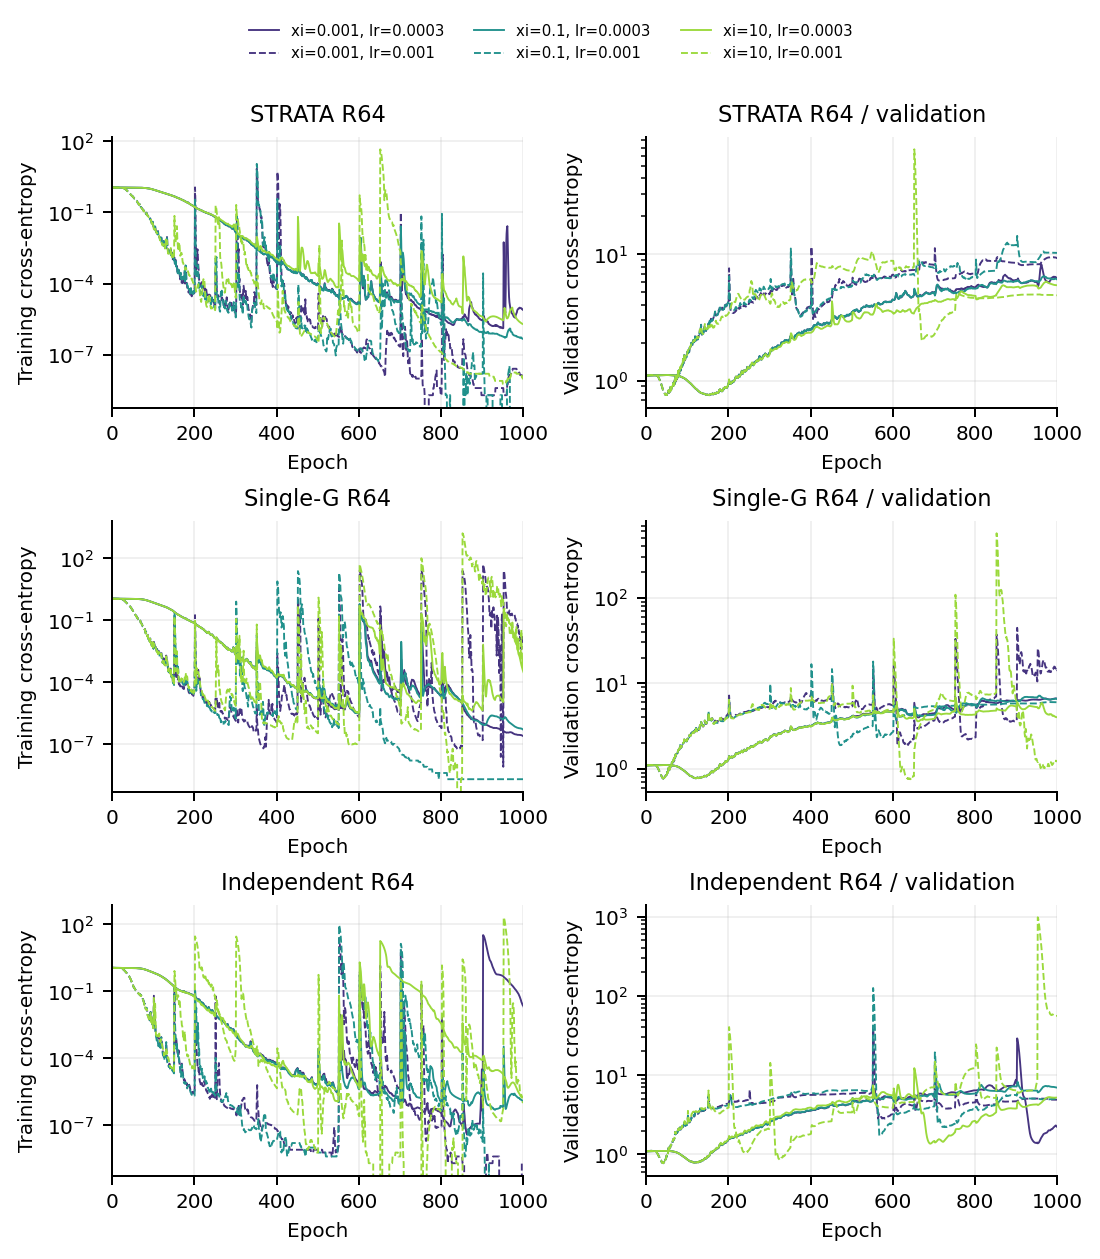
\includegraphics[width=.98\linewidth]{figures/fig_evidence_xi_loss_grid.png}\caption{All 18 completed equal-rank step/rate trajectories, without selection or smoothing. Rows show STRATA, Single-G and Independent; columns show training and validation cross-entropy. Colors denote flag step and line styles distinguish the two learning rates. Every candidate runs 1000 epochs.}\end{figure}
\paragraph{State-matched capacity control.} Same-rank comparisons allocate more optimizer state to STRATA than to Single-Grassmann. We therefore choose the closest integer Single-G rank using initialized tensor storage only, before observing any new accuracy; the target includes probes. Both methods receive the same six-candidate flag-step/rate grid. This is an approximately equal-state comparison, separate from the equal-rank default protocol.
Single-G rank 82 uses 2423128 bytes, versus 2433048 for rank-64 STRATA, a signed difference of -0.408\%. The choice uses exact shape-derived state counts over integer ranks 4--255, including probe-rank saturation, checked against actual initialized storage at four ranks and an archived STRATA final checkpoint; no validation or test score chooses rank.
\begin{table}[htbp]\centering\footnotesize\setlength{\tabcolsep}{3pt}\caption{Completed state-budget control. Rank is fixed from storage alone; every row finishes two rates at each of three flag steps. Default test selects the rate at $\xi=10^{-3}$; six-grid test selects both hyperparameters on validation. Independent uses blocks of dimensions $(16,16,32)$, whose total rank budget is 64. State includes probes and the cached union basis when present.}\label{tab:memory-control}\begin{adjustbox}{max width=\linewidth}
\begin{tabular}{lrrrrr}\toprule Method & State MiB & $\xi_{6}$ & lr$_6$ & Test default & Test six-grid\\\midrule
\rowcolor{oursbg}
STRATA R64 & 2.320 & 10 & 1e-03 & 0.71623 & 0.73383 \\
Single-G R64 & 1.820 & 0.001 & 3e-04 & 0.67902 & 0.67902 \\
Single-G R82 & 2.311 & 0.001 & 1e-03 & 0.72923 & 0.72923 \\
Independent total R64 & 2.195 & 0.001 & 1e-03 & 0.74151 & 0.74151 \\
\bottomrule\end{tabular}
\end{adjustbox}\end{table}
\begin{figure}[!htbp]\centering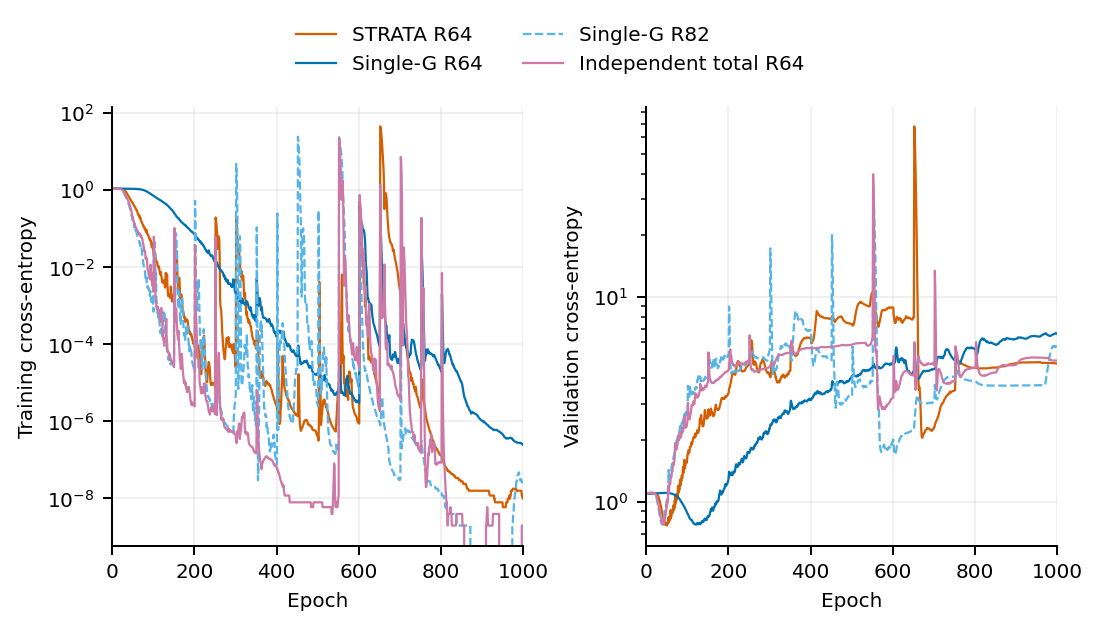
\includegraphics[width=.98\linewidth]{figures/fig_evidence_memory_control.png}\caption{Completed capacity-control training and validation losses after equal six-candidate validation selection. The additional Single-G rank is determined using state storage alone; all six candidates are shown separately below.}\end{figure}
\begin{table}[htbp]\centering\footnotesize\caption{All six completed Single-G state-control candidates. The rank is chosen using storage alone; validation, not test, selects the reported optimum.}\begin{adjustbox}{max width=\linewidth}
\begin{tabular}{rrrr}\toprule $\xi$ & lr & Val acc & Test acc\\\midrule
0.001 & 3e-04 & 0.71554 & 0.71640 \\
0.001 & 1e-03 & 0.73948 & 0.72923 \\
0.1 & 3e-04 & 0.69382 & 0.69613 \\
0.1 & 1e-03 & 0.62916 & 0.61564 \\
10 & 3e-04 & 0.69020 & 0.69950 \\
10 & 1e-03 & 0.72560 & 0.72434 \\
\bottomrule\end{tabular}
\end{adjustbox}\end{table}
\begin{figure}[!htbp]\centering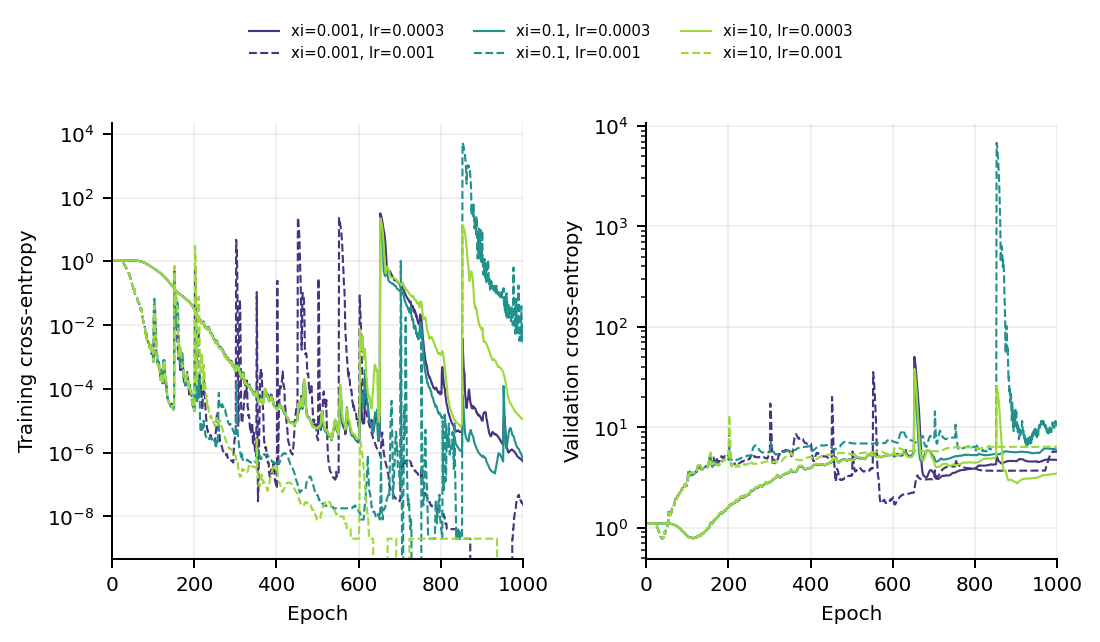
\includegraphics[width=.98\linewidth]{figures/fig_evidence_memory_grid.png}\caption{All six completed Single-G capacity-control training and validation trajectories. No candidate is omitted, selected or smoothed in this grid view.}\end{figure}

\FloatBarrier
\subsection{Completed language and label-shift comparisons}\label{app:language-shift-complete}
\paragraph{Language protocol and endpoint.} All ten WikiText-103/GPT-2-small candidates finish their declared budget before selection. The model has 123849984 parameters and trains from scratch; projected methods use maximum rank 16. Each run uses 1000 units of ten updates, batch size eight and context length 256, totaling 10000 updates and 20480000 training tokens. These are fixed-token-budget comparisons, not 1000-corpus-epoch runs. Each method independently selects between $3\times10^{-4}$ and $10^{-3}$ using mean validation cross-entropy over units 901--1000. Reported perplexity is $\exp(100^{-1}\sum_{u=901}^{1000}\ell_u)$, not the arithmetic mean of per-unit perplexities; the same selected configuration supplies its test endpoint. All candidates use seed 42 and identical frozen token splits. Complete candidate endpoints remain in Appendix~\ref{app:new-completions}.

\begin{table}[htbp]\centering\footnotesize
\caption{\textbf{Completed WikiText-103/GPT-2-small comparison.} Both rates finish for every method. Lower perplexity is better; bold marks the lowest validation and test perplexity. State counts unique final-checkpoint optimizer tensor storage, including probes. Peak is maximum recorded CUDA allocation, a separate quantity.}\label{tab:gpt2-complete}
\begin{tabular}{lrrrrr}\toprule Method & Selected lr & Val PPL & Test PPL & State MiB & Peak MiB\\\midrule
\rowcolor{oursbg}
STRATA & 3e-04 & 143.80 & 144.54 & 38.00 & 4179.2 \\
Single-G & 3e-04 & 139.27 & 139.67 & 29.90 & 4170.2 \\
AdamW & 3e-04 & \textbf{80.11} & \textbf{80.00} & 944.90 & 5081.8 \\
GaLore & 1e-03 & 193.52 & 192.20 & 22.97 & 4164.0 \\
Independent & 3e-04 & 140.90 & 140.81 & 36.84 & 4178.1 \\
\bottomrule\end{tabular}\end{table}

STRATA's test perplexity is 24.8\% lower than GaLore's, but higher than AdamW, Single-Grassmann, and Independent. Its optimizer state is 4.0\% of AdamW's, while its measured peak allocation is 82.2\% of AdamW's. This separates stored-state savings from the weaker held-out result and from peak memory; it does not establish a language-family ranking.
\paragraph{CIFAR-10 label shift.} All ten ResNet-18 fine-tuning configurations finish 1000 epochs. Four consecutive 250-epoch phases upweight classes with label modulo four equal to the phase index by a factor of ten. Validation and test accuracy use the corresponding current-phase weights; the terminal 100 epochs are all in the last phase. Each method independently selects its rate on terminal-100 validation accuracy. STRATA attains 75.012\%, below Single-Grassmann's 76.650\% and the other three methods; the negative comparison is retained. Table~\ref{tab:new-cohorts} includes it in the complete classifier matrix.

\begin{table}[htbp]\centering\footnotesize
\caption{\textbf{Completed CIFAR-10 label-shift comparison.} Validation-selected rates, seed 42, terminal-100 weighted accuracy (percent). Higher accuracy is better. State and peak use the same separate definitions as Table~\ref{tab:gpt2-complete}.}\label{tab:cifar10-shift-complete}
\begin{tabular}{lrrrrr}\toprule Method & Selected lr & Val acc. & Test acc. & State MiB & Peak MiB\\\midrule
\rowcolor{oursbg}
STRATA & 1e-03 & 76.913 & 75.012 & 20.56 & 3151.9 \\
Single-G & 1e-03 & 79.489 & 76.650 & 18.62 & 3154.7 \\
AdamW & 1e-03 & \textbf{81.155} & \textbf{80.212} & 85.25 & 3219.2 \\
GaLore & 1e-03 & 81.096 & 79.996 & 16.44 & 3152.3 \\
Independent & 1e-03 & 78.062 & 76.964 & 20.07 & 3151.4 \\
\bottomrule\end{tabular}\end{table}


\begin{figure}[!htbp]\centering
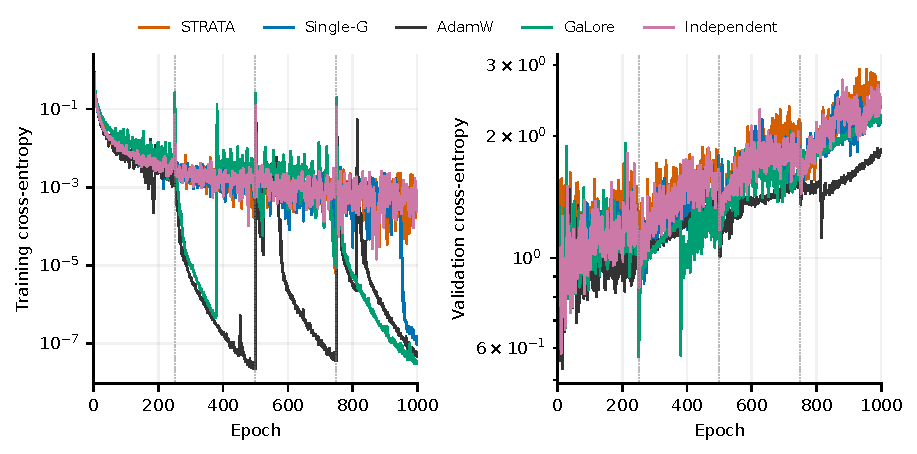
\includegraphics[width=.98\linewidth]{figures/fig_cifar10_shift_complete.pdf}
\caption{\textbf{Completed CIFAR-10 label-shift losses.} Raw training and validation cross-entropy for all five validation-selected configurations. Vertical guides mark phase boundaries at epochs 250, 500, and 750; the validation weighting changes across phases. Every trajectory finishes 1000 epochs. No smoothing or extrapolation.}\label{fig:cifar10-shift-complete}
\end{figure}


\FloatBarrier
\section{Complete Comparison Matrices and Archived Diagnostics}
\label{app:full-empirical-record}
The main-text cases illustrate restricted positive comparisons. This appendix retains the full comparison matrix, archived non-improvements and losses; no result is removed according to its sign. The standard graph matrix contains twelve dataset--architecture settings, of which three improve on Single-Grassmann after the complete two-rate validation search. The other nine remain part of the empirical scope.
\begin{figure}[t]
\centering
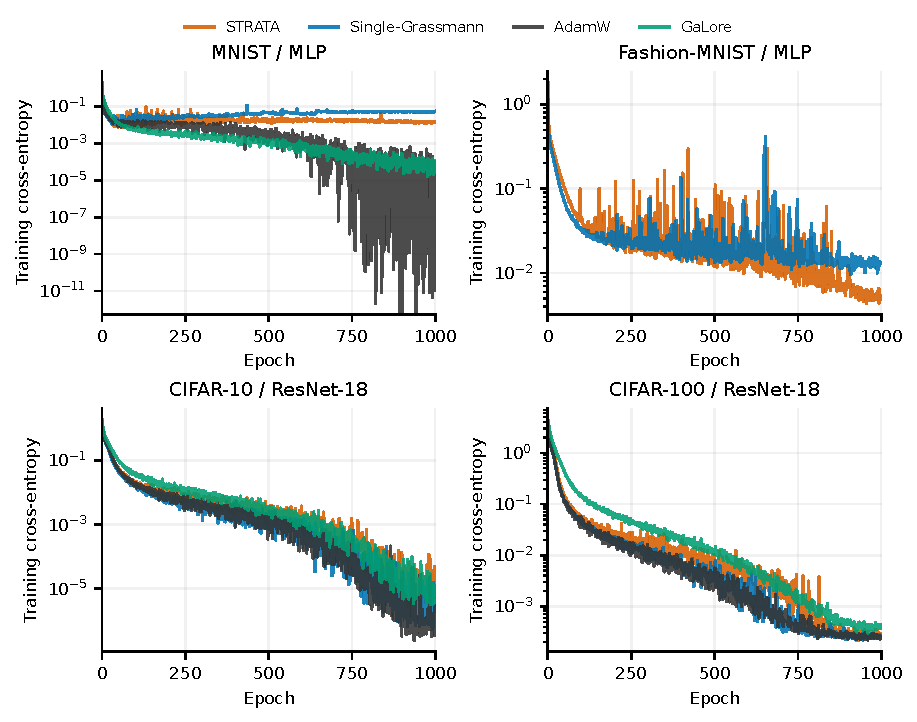
\includegraphics[width=\linewidth]{figures/fig_loss_classification.pdf}
\caption{\textbf{Full 1000-epoch training-loss trajectories.} Four archived classification settings, seed 42. Within each available method grid we select a completed run by terminal-100 validation accuracy and plot its raw training cross-entropy. Baseline grids have unequal sizes; these panels are descriptive convergence comparisons, not an equal-search causal experiment. No smoothing, extrapolation, seed averaging, or test-based selection is used. Training and validation curves for the same runs, every completed classifier-grid loss, fixed-rank PINN curves, graph/continual curves, and separately labeled ongoing runs appear in Appendix~\ref{app:loss-trajectories}.}
\label{fig:loss-classification}
\end{figure}
\paragraph{Loss trajectories and generalization.}
Figure~\ref{fig:loss-classification} replaces endpoint-only inspection with complete recorded optimization paths. Low training cross-entropy does not establish a test-accuracy advantage. The accompanying held-out cross-entropies expose late overfitting and confidence effects that accuracy alone can conceal. Appendix~\ref{app:loss-trajectories} retains both curves and adverse hyperparameter outcomes. All observed epochs are plotted; an archived index of zero is the first logged trained epoch, not a reconstructed common initialization.


\begin{table}[htbp]
\centering
\caption{\textbf{Validation-audited head-to-head endpoints.} PINNs restrict both methods to rank 64 and select by terminal PDE loss. Classifiers select by validation accuracy. Bold compares the two methods; all values use seed 42.}
\label{tab:head-audited}
\begin{adjustbox}{max width=\linewidth}
\begin{tabular}{llrr}
\toprule
Task & Metric & Single-G & STRATA \\
\midrule
burgers & Rel-$L_2$ $\downarrow$ & \textbf{0.02607} & \cellcolor{oursbg}0.02666 \\
burgersg2 & Rel-$L_2$ $\downarrow$ & 0.02617 & \cellcolor{oursbg}\textbf{0.02615} \\
poisson & Rel-$L_2$ $\downarrow$ & 2.04357 & \cellcolor{oursbg}\textbf{0.18741} \\
mnist & Accuracy $\uparrow$ & 0.98011 & \cellcolor{oursbg}\textbf{0.98273} \\
fashion & Accuracy $\uparrow$ & \textbf{0.90328} & \cellcolor{oursbg}0.89907 \\
cifar10 & Accuracy $\uparrow$ & \textbf{0.94034} & \cellcolor{oursbg}0.94014 \\
cifar100 & Accuracy $\uparrow$ & \textbf{0.72574} & \cellcolor{oursbg}0.71402 \\
\bottomrule
\end{tabular}
\end{adjustbox}
\end{table}


\begin{table}[t]
\centering
\caption{Archived benchmark endpoints. Bold marks the better of STRATA and Single-Grassmann only; these are single-seed endpoints, not multi-seed estimates.}
\label{tab:main}
\footnotesize
\begin{adjustbox}{max width=\linewidth}
\begin{tabular}{lrrrrl}
\toprule
Task & AdamW & GaLore & Single-G & STRATA & Verdict \\
\midrule
Burgers rel-$L_2$ $\downarrow$ & 0.0286 & 0.436 & \textbf{0.0261} & \cellcolor{oursbg}0.0267 & tie \\
Burgers-g2 rel-$L_2$ $\downarrow$ & 0.0486 & -- & 0.0262 & \cellcolor{oursbg}\textbf{0.0262} & tie \\
Poisson rel-$L_2$ $\downarrow$ & 0.0079 & -- & 2.0436 & \cellcolor{oursbg}\textbf{0.1874} & SG unstable \\
MNIST acc. $\uparrow$ & 0.987 & 0.985 & 0.9801 & \cellcolor{oursbg}\textbf{0.9827} & tie \\
Fashion acc. $\uparrow$ & -- & -- & \textbf{0.9033} & \cellcolor{oursbg}0.8991 & tie \\
CIFAR-10 acc. $\uparrow$ & 0.9419 & 0.9412 & \textbf{0.9403} & \cellcolor{oursbg}0.9401 & tie \\
CIFAR-100 acc. $\uparrow$ & 0.7358 & 0.7051 & \textbf{0.7257} & \cellcolor{oursbg}0.7140 & SG slight \\
ogbn-arxiv val acc. $\uparrow$ & 0.7351 & 0.7234 & \textbf{0.7349} & \cellcolor{oursbg}0.7337 & tie \\
\bottomrule
\end{tabular}
\end{adjustbox}
\end{table}

\paragraph{Archived comparison.} Table~\ref{tab:main} and Table~\ref{tab:head-audited} support a restrained conclusion. STRATA becomes stable after the numerical fixes, but it is not a universal improvement over Single-Grassmann. In the archived Burgers, Burgers-g2, MNIST, Fashion, CIFAR-10, and ogbn-arxiv comparisons, the practical conclusion is a tie or near-tie. In CIFAR-100, Single-Grassmann is ahead by 0.0117. In Poisson, STRATA is much better than Single-Grassmann in a grid where the latter is unstable, but full AdamW is still substantially better at 0.0079 versus 0.1874.

\begin{table}[htbp]
\centering
\caption{\textbf{Epoch-axis nesting diagnostics.} First/last values and early/late-half means use the complete retained diagnostic trajectory. Spearman $\rho$ uses recorded epochs. Diagnostic trends do not establish a performance ranking.}
\label{tab:dnest}
\begin{adjustbox}{max width=\linewidth}
\begin{tabular}{lrrrrr}
\toprule
Task & First & Last & Early mean & Late mean & $\rho$ \\
\midrule
ogbn-arxiv & 0.047 & 0.493 & 0.330 & 0.477 & +0.998 \\
MNIST & 0.309 & 0.204 & 0.249 & 0.204 & -0.766 \\
Fashion & 0.322 & 0.345 & 0.344 & 0.335 & -0.065 \\
Burgers & 0.880 & 0.690 & 0.416 & 0.618 & +0.901 \\
Poisson & 0.573 & 0.415 & 0.287 & 0.407 & +0.822 \\
CIFAR & 0.512 & 0.601 & 0.397 & 0.434 & +0.224 \\
\bottomrule
\end{tabular}
\end{adjustbox}
\end{table}


\paragraph{$\delta_{\mathrm{nest}}$ is descriptive.} The epoch-axis rejudgment is crucial. Graph is unique only in its low starting point, approximately 0.05, followed by collapse to about 0.49. It is not unique in rising: Burgers and Poisson also rise strongly, with Spearman correlations 0.901 and 0.822, and Burgers after its short initial dip has Spearman 0.993. Because rising, flat, and falling diagnostics all map mostly to head-to-head ties, $\delta_{\mathrm{nest}}$ is useful for describing gradient structure but not for predicting STRATA's performance.

\paragraph{A5 mechanism ablation.} Setting $a_1=\cdots=a_K=a_\perp$ makes $\Gamma^a=0$ in the linear surrogate, while coordinatewise Adam remains basis dependent (Appendix~\ref{app:theory-full}). Equalizing scalar layer weights does not substantially degrade the tested cells: in Burgers at lr $5\times10^{-3}$ and rank 64, full STRATA gives 0.0267 and A5 gives 0.0270; in Poisson at lr $5\times10^{-4}$ and rank 32, full STRATA gives 0.0603 and A5 gives 0.0673. These archived cells alone do not establish a benefit from distinct layer weights. The new PubMed controls below test a different empirical regime, with every intervention and adverse outcome retained.


\paragraph{New complete comparison cohorts.}
Table~\ref{tab:new-cohorts} includes a cohort only when all five methods have completed the stated budget. Two-rate rows require all ten trials before validation-based learning-rate selection; fixed-rate rows use $3\times10^{-4}$ for every method. An incomplete search is not reported as a validation-selected winner.
\begin{table}[t]
\centering\footnotesize
\caption{New full-budget comparison cohorts, seed 42, terminal-100 test accuracy. A two-rate search selects each method using terminal validation accuracy. Fixed-rate rows use no rate selection. Only complete five-method cohorts are shown; the full ledger retains every completed trial.}
\label{tab:new-cohorts}
\setlength{\tabcolsep}{3pt}
\begin{adjustbox}{max width=\linewidth}
\begin{tabular}{llrrrrr}\toprule
Task/model & Protocol & STRATA & Single-G & AdamW & GaLore & Indep.\\\midrule
CiteSeer/gat & 2-rate val & \cellcolor{oursbg}0.5676 & 0.5918 & 0.5737 & \textbf{0.6264} & 0.5718 \\
CiteSeer/gcn & 2-rate val & \cellcolor{oursbg}0.4920 & 0.5156 & 0.5927 & \textbf{0.6166} & 0.5030 \\
CiteSeer/gcnii & 2-rate val & \cellcolor{oursbg}0.4751 & 0.4987 & 0.6085 & \textbf{0.6150} & 0.5042 \\
CiteSeer/sage & 2-rate val & \cellcolor{oursbg}0.5575 & 0.5398 & 0.5530 & \textbf{0.6512} & 0.5584 \\
Cora/gat & 2-rate val & \cellcolor{oursbg}0.6980 & 0.7191 & 0.7100 & \textbf{0.7816} & 0.7365 \\
Cora/gcn & 2-rate val & \cellcolor{oursbg}0.7012 & 0.7164 & 0.7154 & \textbf{0.7718} & 0.6956 \\
Cora/gcnii & 2-rate val & \cellcolor{oursbg}0.6898 & 0.7014 & 0.6784 & \textbf{0.7603} & 0.6934 \\
Cora/sage & 2-rate val & \cellcolor{oursbg}0.4653 & 0.6506 & 0.7060 & \textbf{0.7503} & 0.5641 \\
PubMed/gat & 2-rate val & \cellcolor{oursbg}0.7117 & 0.7431 & 0.7232 & \textbf{0.7663} & 0.7366 \\
PubMed/gcn & 2-rate val & \cellcolor{oursbg}0.7174 & 0.7121 & 0.7045 & \textbf{0.7592} & 0.6878 \\
PubMed/gcnii & 2-rate val & \cellcolor{oursbg}0.6634 & 0.7107 & 0.7088 & \textbf{0.7499} & 0.6693 \\
PubMed/sage & 2-rate val & \cellcolor{oursbg}0.7162 & 0.6790 & 0.6906 & \textbf{0.7580} & 0.7415 \\
adult/MLP-256-256 & 2-rate val & \cellcolor{oursbg}0.8149 & 0.8149 & 0.8172 & \textbf{0.8216} & 0.8117 \\
adult/MLP-512-512 & 2-rate val & \cellcolor{oursbg}0.8151 & 0.8128 & \textbf{0.8191} & 0.8184 & 0.8151 \\
cifar100\_class\_shift/ResNet18-CIFAR & 2-rate val & \cellcolor{oursbg}0.5309 & \textbf{0.5737} & 0.5584 & 0.5306 & 0.5337 \\
cifar10\_label\_shift/ResNet18-CIFAR & 2-rate val & \cellcolor{oursbg}0.7501 & 0.7665 & \textbf{0.8021} & 0.8000 & 0.7696 \\
covertype/MLP-256-256 & 2-rate val & \cellcolor{oursbg}0.9622 & 0.9630 & \textbf{0.9635} & 0.9627 & 0.9615 \\
covertype/MLP-512-512 & 2-rate val & \cellcolor{oursbg}0.9664 & 0.9664 & 0.9645 & 0.9660 & \textbf{0.9675} \\
Rotated-MNIST/MLP (fine-tuning) & 2-rate val & \cellcolor{oursbg}0.5765 & 0.5711 & \textbf{0.6219} & 0.5969 & 0.5728 \\
Rotated-MNIST/MLP (replay) & 2-rate val & \cellcolor{oursbg}0.8858 & 0.8717 & \textbf{0.9072} & 0.8888 & 0.8714 \\
rotated\_mnist\_shift/MLP-256-256 & 2-rate val & \cellcolor{oursbg}0.9761 & 0.9790 & \textbf{0.9806} & 0.9796 & 0.9767 \\
wine\_red/MLP-256-256 & 2-rate val & \cellcolor{oursbg}0.6842 & 0.6883 & 0.7102 & \textbf{0.7185} & 0.6910 \\
wine\_red/MLP-512-512 & 2-rate val & \cellcolor{oursbg}\textbf{0.7150} & 0.6970 & 0.7149 & 0.7105 & 0.7018 \\
wine\_white/MLP-256-256 & 2-rate val & \cellcolor{oursbg}0.7242 & 0.7317 & 0.7204 & 0.7260 & \textbf{0.7389} \\
wine\_white/MLP-512-512 & 2-rate val & \cellcolor{oursbg}0.7088 & 0.7231 & 0.7174 & 0.7100 & \textbf{0.7389} \\
\bottomrule\end{tabular}
\end{adjustbox}\end{table}
After completing both rates on Cora/GCN, validation selects STRATA $3\times10^{-4}$ and Single-Grassmann $10^{-3}$. Their test accuracies are 0.70120 and 0.71643; the earlier positive fixed-rate difference therefore does not survive the completed search. GaLore reaches 0.77180 in this cohort. This adverse comparison is retained.
On the completed PubMed/SAGE two-rate cohort, STRATA reaches 0.71623 versus Single-Grassmann 0.67902, a descriptive gain of 3.721 percentage points. The highest test accuracy among the validation-selected methods is 0.75801 (galore); this single-seed observation does not establish a graph-family advantage.
\paragraph{Completed Rotated-MNIST replay protocol.} Both fine-tuning and replay use the same seed-42 split (55000 training, 5000 validation and 10000 test examples), two 256-wide hidden layers, rank 64, and ten rotations from $0^\circ$ to $90^\circ$ in $10^\circ$ increments. Each rotation receives 100 epochs. Replay stores 200 examples after each task and adds one recalled example per four current-task examples in each minibatch (current batch size 512); all five methods use this same replay rule. Endpoints average epochs 901--1000, evaluating all ten seen rotations. Every method completes both original rates before terminal validation accuracy selects the rate: $10^{-3}$ for STRATA, AdamW, GaLore and Independent, and $3\times10^{-4}$ for Single-Grassmann. STRATA improves on Single-Grassmann by 1.412 percentage points and on Independent by 1.443 points; AdamW and GaLore remain higher. These single-seed comparisons do not establish statistical significance. The loss curves retain all selected methods without smoothing; the mean validation loss covers an increasing set of seen rotations at task boundaries.


\FloatBarrier
\section{Prospective Real-Data Tasks Beyond the Current Cases}
\label{app:prospective-real-tasks}
\paragraph{Purpose and frozen scope.}
The additional study comprises six settings in three directions: ETTh1 and ETTh2 forecasting, MovieLens100K and MovieLens1M explicit-rating prediction, and gas-sensor drift with fine-tuning or replay. The task list, data digests, splits, models, six candidates per method, metrics and failure policy are frozen before formal outcomes in the retained plan. The goal is to test structured-gradient and adaptation hypotheses beyond citation graphs; neither dataset readiness nor a queued configuration is evidence of improvement. We retain all declared settings and candidate failures, irrespective of the sign of the result.

\paragraph{ETT forecasting.}
We use the original hourly transformer series~\citep{zhou2021informer}, each with seven numeric channels. The first $8640$ observations define training; validation and test targets lie in $[8640,11520)$ and $[11520,14400)$, respectively. The remaining observations do not enter these trials. With lookback $L=96$ and horizon $H=24$, a split $[a,b)$ contains precisely
\[
 t\in\{\max(a,L),\ldots,b-H\},\qquad
 x_t=\operatorname{vec}(z_{t-L:t}),\quad
 y_t=\operatorname{vec}(z_{t:t+H}).
\]
Thus an input uses past observations only, and every target horizon is contained in its own split. Channel means and standard deviations use the training prefix only. The common forecaster is a $672\to256\to256\to168$ MLP with GELU hidden activations. Its primary metric is MSE in training-standard-deviation units; MAE is secondary. These are controlled optimizer comparisons on ETT data, not claims to reproduce the Informer architecture or a forecasting state-of-the-art endpoint.

\paragraph{Explicit-rating recommendation.}
MovieLens100K and MovieLens1M come from the official GroupLens releases~\citep{harper2015movielens}. MovieLens100K preserves the official \texttt{u1.test}; a SHA-256 user/item hash assigns ten percent of \texttt{u1.base} to validation, yielding $71978/8022/20000$ ratings. MovieLens1M uses chronological $70/15/15$ splits within each user, with item ID breaking timestamp ties, yielding $697378/149931/152900$ ratings. User/item pairs do not overlap across splits. Catalog IDs may be known without using held-out ratings. All methods fit the same biased matrix-factorization model,
\[
 \widehat r_{ui}=\mu_{\rm train}+b_u+c_i+
 \frac{p_u^\top q_i}{\sqrt{128}},\qquad p_u,q_i\in\mathbb R^{128}.
\]
Training minimizes observed-rating MSE. The primary evaluation is raw-rating RMSE; these tasks do not support a top-$k$ retrieval or NDCG claim. Embeddings use dense gradients, so every optimizer sees the same parameterization and examples. Complete epochs traverse all training ratings.

\paragraph{Real sensor drift.}
The UCI Gas Sensor Array Drift data~\citep{vergara2012gasdrift} contain $13910$ records, $128$ features, six labels and ten ordered batches. A global SHA-256 hash of the float32 feature row and label fixes $70/15/15$ training/validation/test roles; identical records keep the same role across batches. Only batch-one training rows determine feature normalization. The common classifier is a $128\to256\to256\to6$ ReLU MLP. Training spends $100$ complete epochs in each successive domain, for $1000$ total epochs, and never trains on future domains. Fine-tuning uses current-domain training rows. Replay additionally samples at most $128$ old examples per current minibatch from a deterministic $512$-example sample of past training domains, refreshed at domain boundaries. This is the replay sample size, not a claim that the resident benchmark arrays consume constant storage. Flags and moments carry across domain switches. Evaluation at domain $k$ averages the per-domain held-out accuracies equally,
\[
 A_k(\theta)=\frac1k\sum_{j=1}^k
 \frac1{|D_j|}\sum_{(x,y)\in D_j}
 \mathbf1\{\arg\max f_\theta(x)=y\}.
\]
Per-domain accuracies are retained. Since the set of seen domains grows, these curves are not measurements of convergence to one fixed population objective.

\paragraph{Equal search counts and computational budgets.}
STRATA, Single-Grassmann and Independent use maximum/total rank $32$ and six candidates,
\[
 \eta\in\{3\times10^{-4},10^{-3}\},\qquad
 \xi\in\{10^{-3},10^{-1},10\}.
\]
Independent's actual block dimensions are $(8,8,16)$, totaling $32$. AdamW and GaLore each use six distinct learning rates,
\[
 \eta\in\{10^{-4},3\times10^{-4},10^{-3},3\times10^{-3},10^{-2},3\times10^{-2}\}.
\]
Thus the search counts are equal; the hyperparameter spaces are explicitly different. These are comparisons of the full algorithms, not a pure isolated nesting intervention. All use seed42, float32 computation, clipping at norm10 and zero weight decay. A cosine schedule with five-epoch warmup spans the full static task, or restarts within each $100$-epoch drift domain. Each prescribed epoch traverses the complete relevant training set. Six CPU workers use two intra-op threads each after checking capacity; CPU wall time is shared-server timing, and a zero CUDA-allocation field means not applicable, not zero total memory. State counts include fixed probes and persistent buffers.

\paragraph{Selection and complete reporting.}
For every method and setting, the selected candidate optimizes the mean primary validation metric over the terminal $100$ epochs: MSE/RMSE is minimized and accuracy maximized. Test metrics never select a configuration. The same reporting rule applies to favorable and unfavorable results. A setting is summarized only after its $30$ candidates complete or record a failure; a failed candidate has no fabricated endpoint, and a method with no complete candidate has no selected score. Raw losses, validation/test metrics, flag snapshots, ten-epoch checkpoints, source hashes and data hashes remain available. Small smoke checks are stored separately and excluded from the formal queue. The single-seed protocol does not justify statistical-significance claims or a guaranteed winner in any task family.

\paragraph{Relation to the conditional theory.}
Replay makes persistent past-domain corrections available alongside current-domain gradients while preserving the model architecture and optimizer tensor-state sizes. The fine-tuning/replay contrast therefore probes a data-regime interaction; it does not isolate a geometric component of the optimizer. ETT windows overlap, chronological ratings share users and sensor domains are dependent and shifted. These data do not by themselves establish the sampling assumptions of the generalization theorems, and unclipped MSE is not a bounded loss. The task comparisons are empirical tests of optimization and state--quality tradeoffs, not numerical certificates of the conditional convergence or generalization bounds.

\subsection{Prospective new-task execution and complete comparisons}\label{app:new-family-results}
This extension was declared before its outcomes: six settings, five methods and six candidates per method. Every formal run uses seed 42 and 1000 complete epochs. Configuration selection uses terminal-100 validation metrics. A comparison appears only after all 30 declared candidates have completed or recorded failure; failures have no fabricated endpoint. A method with no complete candidate has no selected score. Negative outcomes and every declared setting remain in this record.
\begin{table}[htbp]\centering\footnotesize\setlength{\tabcolsep}{3pt}\caption{Execution coverage of every declared new setting. Counts are configurations, not quality wins; failed candidates remain visible.}\begin{adjustbox}{max width=\linewidth}
\begin{tabular}{llrrrr}\toprule Family & Setting & Complete & Running & Pending & Failed\\\midrule
forecasting & ETTh1 / H24 & 30 & 0 & 0 & 0 \\
forecasting & ETTh2 / H24 & 30 & 0 & 0 & 0 \\
recommendation & MovieLens100K / ratings & 30 & 0 & 0 & 0 \\
recommendation & MovieLens1M / ratings & 30 & 0 & 0 & 0 \\
sensor\_drift & Gas sensors / fine-tuning & 30 & 0 & 0 & 0 \\
sensor\_drift & Gas sensors / replay & 30 & 0 & 0 & 0 \\
\bottomrule\end{tabular}
\end{adjustbox}\end{table}
\FloatBarrier
{\footnotesize\setlength{\tabcolsep}{3pt}\begin{longtable}{llrrrrr}\caption{All fully searched new settings. Each displayed method independently selects among six candidates on validation. Values are terminal-100 test metrics; MSE and RMSE are lower-is-better, accuracy is higher-is-better. No setting is omitted according to outcome.}\label{tab:new-families-complete}\\\toprule Setting & Metric & STRATA & Single-G & AdamW & GaLore & Indep.\\\midrule\endfirsthead\toprule Setting & Metric & STRATA & Single-G & AdamW & GaLore & Indep.\\\midrule\endhead
ETTh1 / H24 & MSE & \cellcolor{oursbg}0.89922 & 0.88655 & 0.86679 & \textbf{0.76942} & 0.90163 \\
ETTh2 / H24 & MSE & \cellcolor{oursbg}\textbf{1.74404} & 2.37970 & 2.16884 & 1.79170 & 2.18874 \\
MovieLens100K / ratings & RMSE & \cellcolor{oursbg}0.96949 & 1.00529 & \textbf{0.93295} & 0.95778 & 1.01755 \\
MovieLens1M / ratings & RMSE & \cellcolor{oursbg}1.05052 & 1.09444 & 0.98066 & \textbf{0.91712} & 1.08146 \\
Gas sensors / fine-tuning & acc & \cellcolor{oursbg}0.85453 & 0.85375 & 0.82335 & \textbf{0.90656} & 0.80659 \\
Gas sensors / replay & acc & \cellcolor{oursbg}0.96506 & 0.96409 & \textbf{0.96536} & 0.96232 & 0.96343 \\
\bottomrule\end{longtable}}
\clearpage
\paragraph{ETTh1 / H24 complete search.} Primary metric: MSE. Recorded candidate failures: STRATA 0, Single-G 0, AdamW 0, GaLore 0, Independent 0. Shared-CPU wall time is not isolated throughput; tensor-state size is distinct from peak memory.
\begin{table}[htbp]\centering\caption{\textbf{ETTh1 / H24: selected configurations and stored state.} Each method selects among six candidates on validation. Bold marks the best validation/test value; the green row identifies STRATA. Pareto status uses test quality and stored state, not peak memory.}\begin{adjustbox}{max width=\linewidth}
\begin{tabular}{lrrrrrl}\toprule Method & lr & $\xi$ & Val & Test & State MiB & Pareto\\\midrule
\rowcolor{oursbg}
STRATA & 3e-04 & 0.001 & 0.91637 & 0.89922 & 0.792 & \rwcross \\
Single-G & 3e-04 & 0.001 & 1.06275 & 0.88655 & 0.585 & \rwcross \\
AdamW & 1e-02 & -- & 0.94111 & 0.86679 & 2.146 & \rwcross \\
GaLore & 1e-04 & -- & \textbf{0.73812} & \textbf{0.76942} & 0.377 & \rwcheck \\
Independent & 3e-04 & 0.1 & 1.04792 & 0.90163 & 0.751 & \rwcross \\
\bottomrule\end{tabular}
\end{adjustbox}\end{table}
\begin{figure}[!htbp]\centering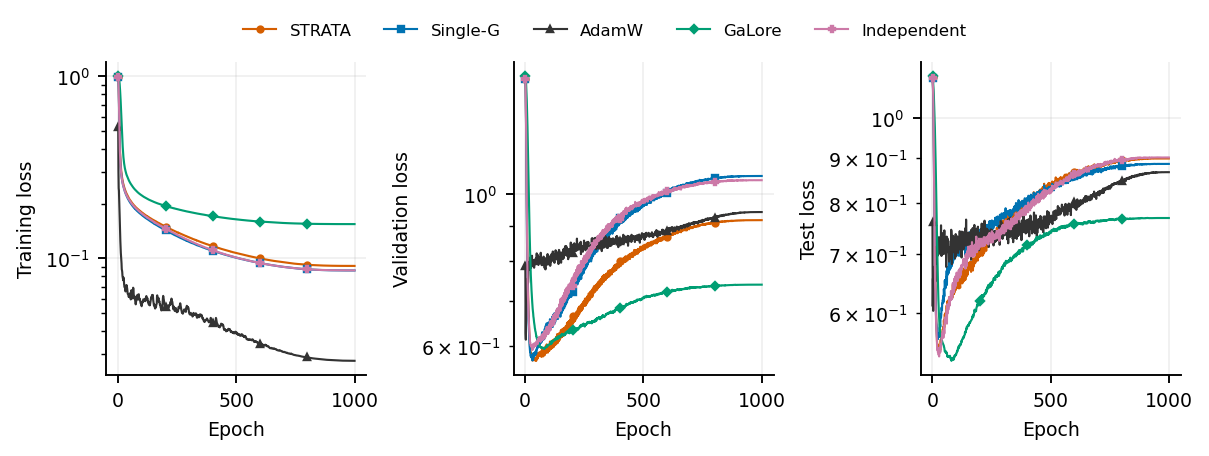
\includegraphics[width=.98\linewidth]{figures/fig_new_family_edb567be48.png}\caption{Complete ETTh1 / H24 loss trajectories. Left to right: training, validation, and test loss. Selection uses validation only after all candidates finish or record failure. All five methods and adverse outcomes remain visible. Curves are raw and unsmoothed.}\end{figure}
\clearpage
\paragraph{ETTh2 / H24 complete search.} Primary metric: MSE. Recorded candidate failures: STRATA 0, Single-G 0, AdamW 0, GaLore 0, Independent 0. Shared-CPU wall time is not isolated throughput; tensor-state size is distinct from peak memory.
\begin{table}[htbp]\centering\caption{\textbf{ETTh2 / H24: selected configurations and stored state.} Each method selects among six candidates on validation. Bold marks the best validation/test value; the green row identifies STRATA. Pareto status uses test quality and stored state, not peak memory.}\begin{adjustbox}{max width=\linewidth}
\begin{tabular}{lrrrrrl}\toprule Method & lr & $\xi$ & Val & Test & State MiB & Pareto\\\midrule
\rowcolor{oursbg}
STRATA & 3e-04 & 10 & 0.85177 & \textbf{1.74404} & 0.792 & \rwcheck \\
Single-G & 3e-04 & 0.1 & \textbf{0.80694} & 2.37970 & 0.585 & \rwcross \\
AdamW & 3e-03 & -- & 1.25122 & 2.16884 & 2.146 & \rwcross \\
GaLore & 1e-02 & -- & 1.00745 & 1.79170 & 0.377 & \rwcheck \\
Independent & 1e-03 & 0.1 & 1.31254 & 2.18874 & 0.751 & \rwcross \\
\bottomrule\end{tabular}
\end{adjustbox}\end{table}
\begin{figure}[!htbp]\centering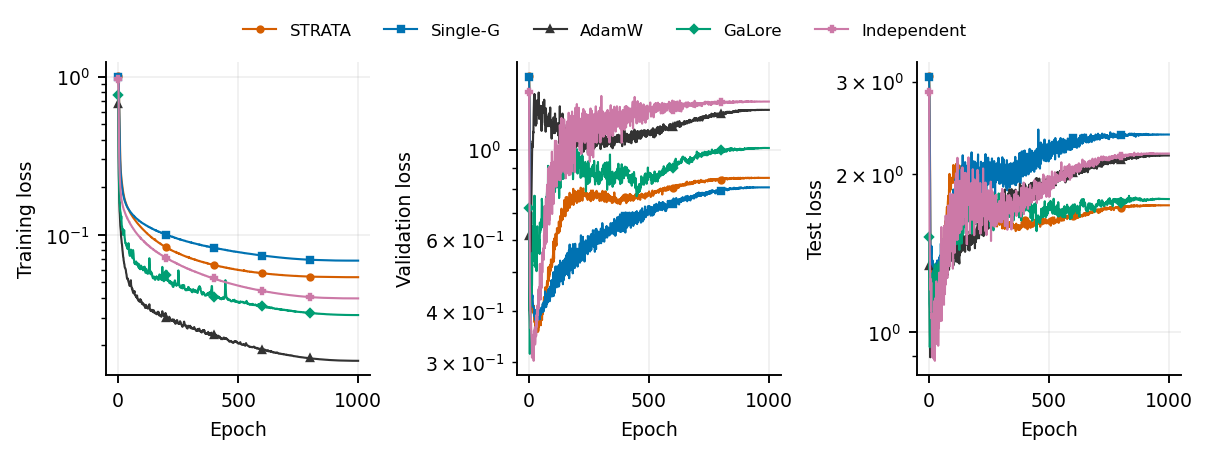
\includegraphics[width=.98\linewidth]{figures/fig_new_family_151c40f1dd.png}\caption{Complete ETTh2 / H24 loss trajectories. Left to right: training, validation, and test loss. Selection uses validation only after all candidates finish or record failure. All five methods and adverse outcomes remain visible. Curves are raw and unsmoothed.}\end{figure}
\clearpage
\paragraph{MovieLens100K / ratings complete search.} Primary metric: RMSE. Recorded candidate failures: STRATA 0, Single-G 0, AdamW 0, GaLore 0, Independent 0. Shared-CPU wall time is not isolated throughput; tensor-state size is distinct from peak memory.
\begin{table}[htbp]\centering\caption{\textbf{MovieLens100K / ratings: selected configurations and stored state.} Each method selects among six candidates on validation. Bold marks the best validation/test value; the green row identifies STRATA. Pareto status uses test quality and stored state, not peak memory.}\begin{adjustbox}{max width=\linewidth}
\begin{tabular}{lrrrrrl}\toprule Method & lr & $\xi$ & Val & Test & State MiB & Pareto\\\midrule
\rowcolor{oursbg}
STRATA & 3e-04 & 10 & 0.96257 & 0.96949 & 0.848 & \rwcross \\
Single-G & 3e-04 & 10 & 1.00521 & 1.00529 & 0.770 & \rwcross \\
AdamW & 1e-04 & -- & \textbf{0.91533} & \textbf{0.93295} & 2.584 & \rwcheck \\
GaLore & 1e-04 & -- & 0.94025 & 0.95778 & 0.692 & \rwcheck \\
Independent & 3e-04 & 10 & 1.00684 & 1.01755 & 0.833 & \rwcross \\
\bottomrule\end{tabular}
\end{adjustbox}\end{table}
\begin{figure}[!htbp]\centering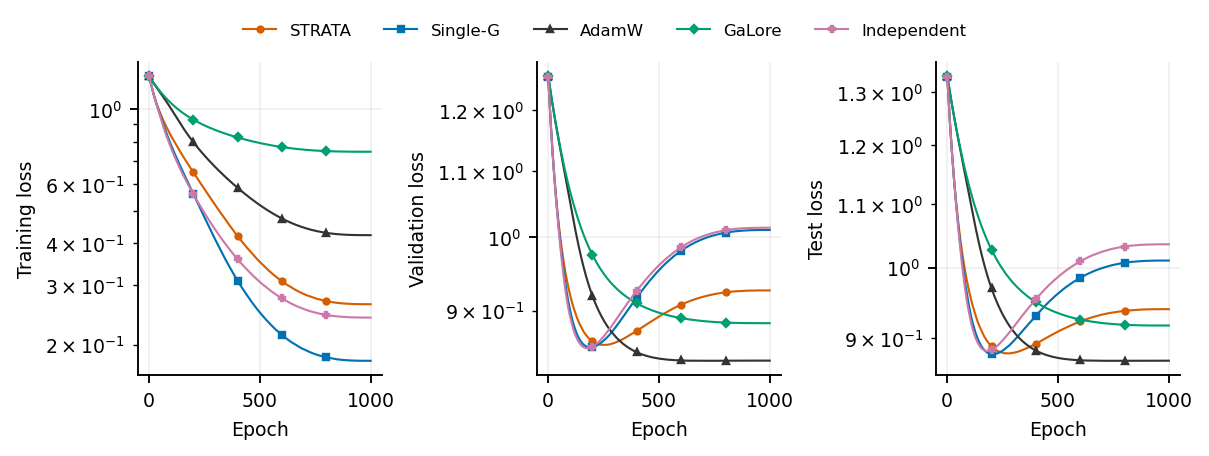
\includegraphics[width=.98\linewidth]{figures/fig_new_family_ce752a0fe4.png}\caption{Complete MovieLens100K / ratings loss trajectories. Left to right: training, validation, and test loss. Selection uses validation only after all candidates finish or record failure. All five methods and adverse outcomes remain visible. Curves are raw and unsmoothed.}\end{figure}
\clearpage
\paragraph{MovieLens1M / ratings complete search.} Primary metric: RMSE. Recorded candidate failures: STRATA 0, Single-G 0, AdamW 0, GaLore 0, Independent 0. Shared-CPU wall time is not isolated throughput; tensor-state size is distinct from peak memory.
\begin{table}[htbp]\centering\caption{\textbf{MovieLens1M / ratings: selected configurations and stored state.} Each method selects among six candidates on validation. Bold marks the best validation/test value; the green row identifies STRATA. Pareto status uses test quality and stored state, not peak memory.}\begin{adjustbox}{max width=\linewidth}
\begin{tabular}{lrrrrrl}\toprule Method & lr & $\xi$ & Val & Test & State MiB & Pareto\\\midrule
\rowcolor{oursbg}
STRATA & 3e-04 & 0.001 & 1.03092 & 1.05052 & 2.703 & \rwcross \\
Single-G & 3e-04 & 0.001 & 1.07528 & 1.09444 & 2.625 & \rwcross \\
AdamW & 1e-04 & -- & 0.96096 & 0.98066 & 9.834 & \rwcross \\
GaLore & 1e-04 & -- & \textbf{0.89748} & \textbf{0.91712} & 2.547 & \rwcheck \\
Independent & 3e-04 & 10 & 1.05453 & 1.08146 & 2.688 & \rwcross \\
\bottomrule\end{tabular}
\end{adjustbox}\end{table}
\begin{figure}[!htbp]\centering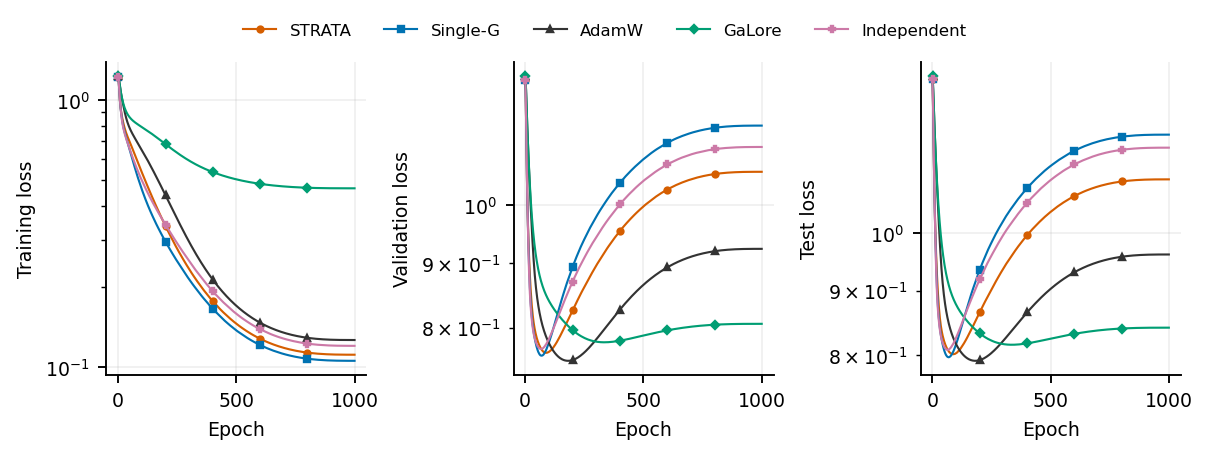
\includegraphics[width=.98\linewidth]{figures/fig_new_family_4338a23ff7.png}\caption{Complete MovieLens1M / ratings loss trajectories. Left to right: training, validation, and test loss. Selection uses validation only after all candidates finish or record failure. All five methods and adverse outcomes remain visible. Curves are raw and unsmoothed.}\end{figure}
\clearpage
\paragraph{Gas sensors / fine-tuning complete search.} Primary metric: acc. Recorded candidate failures: STRATA 0, Single-G 0, AdamW 0, GaLore 0, Independent 0. Shared-CPU wall time is not isolated throughput; tensor-state size is distinct from peak memory.
\begin{table}[htbp]\centering\caption{\textbf{Gas sensors / fine-tuning: selected configurations and stored state.} Each method selects among six candidates on validation. Bold marks the best validation/test value; the green row identifies STRATA. Pareto status uses test quality and stored state, not peak memory.}\begin{adjustbox}{max width=\linewidth}
\begin{tabular}{lrrrrrl}\toprule Method & lr & $\xi$ & Val & Test & State MiB & Pareto\\\midrule
\rowcolor{oursbg}
STRATA & 1e-03 & 0.1 & 0.86518 & 0.85453 & 0.422 & \rwcross \\
Single-G & 3e-04 & 0.001 & 0.85400 & 0.85375 & 0.305 & \rwcross \\
AdamW & 3e-03 & -- & 0.85438 & 0.82335 & 0.766 & \rwcross \\
GaLore & 1e-03 & -- & \textbf{0.90496} & \textbf{0.90656} & 0.188 & \rwcheck \\
Independent & 3e-04 & 10 & 0.82691 & 0.80659 & 0.398 & \rwcross \\
\bottomrule\end{tabular}
\end{adjustbox}\end{table}
\begin{figure}[!htbp]\centering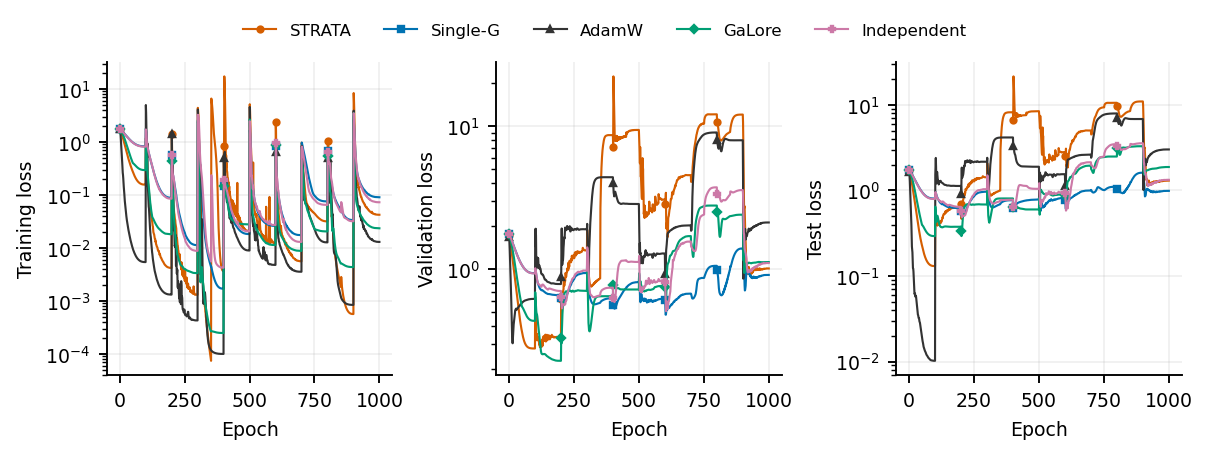
\includegraphics[width=.98\linewidth]{figures/fig_new_family_2d8b18f1f2.png}\caption{Complete Gas sensors / fine-tuning loss trajectories. Left to right: training, validation, and test loss. Selection uses validation only after all candidates finish or record failure. All five methods and adverse outcomes remain visible. Curves are raw and unsmoothed; sensor-drift evaluation averages domains seen so far and changes at domain boundaries.}\end{figure}
\clearpage
\paragraph{Gas sensors / replay complete search.} Primary metric: acc. Recorded candidate failures: STRATA 0, Single-G 0, AdamW 0, GaLore 0, Independent 0. Shared-CPU wall time is not isolated throughput; tensor-state size is distinct from peak memory.
\begin{table}[htbp]\centering\caption{\textbf{Gas sensors / replay: selected configurations and stored state.} Each method selects among six candidates on validation. Bold marks the best validation/test value; the green row identifies STRATA. Pareto status uses test quality and stored state, not peak memory.}\begin{adjustbox}{max width=\linewidth}
\begin{tabular}{lrrrrrl}\toprule Method & lr & $\xi$ & Val & Test & State MiB & Pareto\\\midrule
\rowcolor{oursbg}
STRATA & 1e-03 & 10 & \textbf{0.97487} & 0.96506 & 0.422 & \rwcheck \\
Single-G & 1e-03 & 0.001 & 0.96936 & 0.96409 & 0.305 & \rwcheck \\
AdamW & 3e-03 & -- & 0.97452 & \textbf{0.96536} & 0.766 & \rwcheck \\
GaLore & 1e-03 & -- & 0.97444 & 0.96232 & 0.188 & \rwcheck \\
Independent & 1e-03 & 10 & 0.97214 & 0.96343 & 0.398 & \rwcross \\
\bottomrule\end{tabular}
\end{adjustbox}\end{table}
\begin{figure}[!htbp]\centering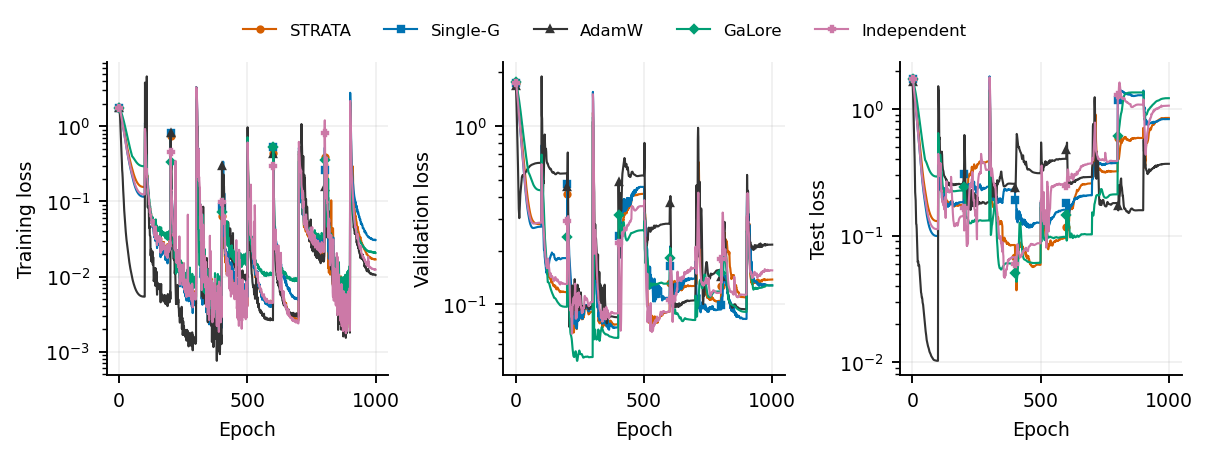
\includegraphics[width=.98\linewidth]{figures/fig_new_family_8ed4986eff.png}\caption{Complete Gas sensors / replay loss trajectories. Left to right: training, validation, and test loss. Selection uses validation only after all candidates finish or record failure. All five methods and adverse outcomes remain visible. Curves are raw and unsmoothed; sensor-drift evaluation averages domains seen so far and changes at domain boundaries.}\end{figure}

